%\documentclass[12pt, twocolumn]{article}
%\documentclass[12pt, openany]{book}
\documentclass[12pt, oneside]{book}
%\usepackage{fullpage}           % makes all margins 1 inch?
\topmargin=-1.0cm
\textheight=23cm
\evensidemargin=-1.0cm
\oddsidemargin=-1.0cm
\textwidth=19cm
\setcounter{secnumdepth}{-1}  % suppress numbering of sections
\usepackage{amsmath}
\usepackage{amssymb}          % for mathbb
\usepackage{hyperref}

\usepackage{comment}          
% to comment out larger sections via \begin{comment} ... \end{comment} 
% see:
% https://tex.stackexchange.com/questions/17816/commenting-out-large-sections
% https://tex.stackexchange.com/questions/11177/how-to-write-hidden-notes-in-a-latex-file/73418

%\DeclareMathOperator{\d}{d}                  % exterior derivative

%\let\cleardoublepage\clearpage

\begin{document}
	
% formatting:
\parindent=0in
\parskip=0pt
\pagenumbering{roman}
		
% main text
\pagenumbering{arabic} \setcounter{page}{1}

\author{Robin Schmidt}

\title{Mathematical Recipes for Scientists, Engineers and Programmers}
\maketitle
\tableofcontents

%\chapter{Basics}
\chapter{Basics}
Mathematics is a broad subject and I would be way out of my depth to try to give a definition what it actually is. I like to think of it as the study of structures, patterns and equivalences and as a way to systematize, formalize and eventually automate thought processes. One big theme is to figure out, under which circumstances one thing is equal to another. Often, there are multiple ways to compute the same thing and a big sub-theme of finding equivalences is to find computational shortcuts that allow to do a computation more efficiently than was previously possible. The body of mathematical knowledge today is an impressive tower of known facts about abstract constructs of the human mind. The first of these abstract constructs that one usually encounters in elementary school is the idea of a natural number and one learns how to add, subtract, multiply and divide them. Building on that, one later encounters negative numbers, rational numbers, real numbers and complex numbers. I like to think of numbers as the ground floor of the tower. Numbers usually set the stage for doing mathematics on first encounter, but the foundations of mathematics can go down to even lower levels: If numbers are the ground floor, then it may be appropriate to think of set theory and mathematical logic as two basement floors. Having numbers in place, one can go up a stage and look at functions that map numbers to other numbers. One then may realize that addition, multiplication, etc. are actually functions, too: they take two inputs and map them to a single output. Such generalization with hindsight is also a common theme in math. A stage higher, you can look at mappings that map functions to other functions. And it goes ever higher up. Well, actually, it also kind of branches out while going up, so maybe a tree of knowledge might be better analogy than a tower - but then the roots (levels below ground) do not branch out as much as the upper levels. But there certainly is some sort of trunk that everybody needs to know. This trunk contains numbers themselves (from the natural to the complex ones), equations (and solution techniques for them when they contain unknowns), elementary functions (polynomial, rational, exponential, trigonometric and their inverses), linear algebra (vectors, matrices, linear systems of equations) and single variable calculus (derivatives, integrals, differential equations). With these basics in place, math branches out into various directions. Some of these are: multivariable calculus: the study of functions of several variables, abstract algebra: generalizes ideas such as addition, multiplication, etc. to other sorts of objects and identifies the common structure, number theory: studies natural numbers and especially prime numbers in depth, functional analysis: studies functions of functions, topology: studies qualitative properties of shapes, etc. 

\paragraph{Goals and Audience}
This document is an attempt to give a condensed high level overview about what's going on in a particular subject and to give a comprehensive catalog of formulas, recipies and algorithms to actually get the work done. There is little regard to derivation or justification and no regard whatsoever to proof or mathematical rigor. It's meant to be a collection of recipies for the practitioner who needs to use math in applications. In focus are the questions: What is it? What can I do with it? How can I do it? The focus is deliberately not: Why does it work the way it does? That would fill volumes (and has done so) and thereby just distract from getting the work done. The scope is broad but shallow. I don't want to drown the reader in details of derivations. If you are looking for a detailed, in depth understanding, you will need to consult actual math textbooks. This book here should serve more as a launchpad and give you the right keywords to serach for.  Despite being shallow with regard to derivations (and therefore understanding), I strive to be comprehensive with regard to listing potentially important formulas and recipes. It's more like a cheat-sheet. I try to minimize using forward references, i.e. references to material that is only covered in later chapters. But in some cases, these are inavoidable. The body of math knowledge is actually even more complicated than a tree. Past the bottom layers, it's more like a vast interconnected network where everything hangs together, so putting it in a strict linear order from bottom to top is difficult. I'll try nonetheless. The material is organized as follows: Part 1 deals with basics, linear algebra, calculus and geometry - roughly speaking, the world of continuous mathematics. Part 2 is devoted to discrete mathematics... Part 3 is devoted to applications.... tbc...



% Latex output is a bit ugly - only one line on a full page!



\subsection{Set Theory}
Set theory is often said to be the foundation of all mathematics - even much more fundamental than the natural numbers. 
%In fact, it is possible to "construct" the natural numbers from sets. We will not go down this road though, since this is not really relevant in applied math. 
The idea of a set was initially introduced by Georg Cantor in an intuitive way. His way of establishing set theory later turned out to have some flaws which is why it was later rebuilt more formally. The result of this rebuild is called "axiomatic set theory" and is very abstract and formal. Fortunately, Cantor's view, which is today sometimes called "naive set theory", is good enough for us - at least for the time being. 

\subsubsection{Sets}
In Cantor's definition "A set is a gathering together into a whole of definite, distinct objects of our perception or of our thought which are called elements of the set.". So, in essence, a set is just a bunch of things. A very general concept indeed. Sets are usually denoted in curly braces. For example, the set of the 3 letters $a,b,c$ would be denoted as $\{a,b,c\}$. Two sets are considered equal, if and only if they contain the same elements. It does not matter in which order the elements are written down or if an element appears multiple times. So that means, for example, the sets $\{c,a,b\}$ or $\{a,c,a,a,b,c\}$ are in fact equal to the set $\{a,b,c\}$. By the way, the phrase "if and only if" appears sufficiently often in math texts that some authors use the abbreviation "iff" for that - yes, that's an "if" with a double-f. I may sometimes use that, too. Sets can be given names. For example, we may call our set above $S$ and we may write this as $S = \{a,b,c\}$. Element membership is denoted by an $\in$ symbol, so to express the fact that $b$ is an element of the set $S$, we would write $b \in S$. If we want to express that a certain object, say $d$, is not an element of a set $S$, we write this as $d \notin S$.

%\medskip 
\paragraph{Sets of Sets}
Sets can have other sets as elements and that nesting capability can be used recursively to build arbitrarily complex structures purely from sets. These structures also include the number systems that are used in math. For example, the number zero can be represented by the empty set: $0 = \{\}$, which is also denoted by $\emptyset$, the number one by the set that contains the empty set (i.e. zero): $1 = \{ 0 \} =  \{ \emptyset \}$, the number two by the set that contains zero and one: $2 = \{ 0, 1 \} = \{ \emptyset, \{ \emptyset \} \}$ and so on. Of course, that's super tedious and nobody actually thinks about numbers this way - but in principle, it can be done. Note that in this context $\emptyset$ and $\{ \emptyset \}$ are different things. The first is the empty set and the second is the set that contains the empty set. The nesting matters. One is an empty box, the other one is a box that contains something: namely, an empty box. If you really go down to the very lowest levels of math, then sets are actually the \emph{only} things that can occur as elements of (other) sets because sets are really the only thing that exists in this world. There is nothing else but sets and all the rich and complex mathematical structures that exist can, in principle, be built recursively from these sets. 
%[VERIFY!]

%\medskip 
\paragraph{Set Builder Notation}
In math, the sets we are dealing with are often sets of numbers and they may have many or even infinitely many elements. To denote very large or infinite sets compactly there are notations based on predicate logic. For example to denote the set of all numbers larger than 100 but less than 1000, we may write $\{x : x > 100 \wedge x < 1000\}$. but now we are getting ahead of ourselves. To understand that notation, we actually first have to understand what $>$ and $<$ means. I'm pretty sure, you already do know what they mean, namely, \emph{less than} and \emph{greater than} but in the context of set theory, these symbols first need to be defined, too. To do so, we need to first define what an order relation is. We'll look at these soon. Generally, this kind of notation to define a set is called set builder notation and specifies a set by listing some properties that elements of the set must satisfy. In this notation, we use a placeholder or variable, here $x$, which stands in for some generic element of the set, then use a colon (or, alternatively a vertical bar) and then list the properties that this element should satisfy. So, a set defined by set builder notation generally look like: $\{x : P(x)\}$ or  $\{x \; | \; P(x)\}$ where $P(x)$ is some property or predicate that can be expressed using the machinery of predicate logic. [TODO: maybe use $\varphi$ instead of $P$]

% Maybe use 

% Soo - which of the two notations should we use in this book? The vertical bar looks more aesthetic but I have used the colon already in a few places and its also easier to typeset because we don't nee the spaces \; ..hmmmm

%https://en.wikipedia.org/wiki/Set-builder_notation

\subsubsection{Tuples}
Sometimes, we may want to model situations in which the order of entries actually does matter. Sets are per definition not suitable for this (at least not directly), so we need something else. That other thing is the tuple. A tuple is typically denoted by listing the entries in parentheses. The 3-tuple $(a,b,c)$ is not equal to $(c,a,b)$. Tuples with two elements are also called ordered pairs, 3-tuples triples, 4-tuples quadruples and 5-tuples quintuples. For brevity, in the following, I will just say "pair" when I mean "ordered pair", i.e. pairs are implicitly always assumed to be ordered. When we talk about a tuple, the entries are no longer called "elements" but instead \emph{coordinates} or \emph{components}. If you really want to be puristic and build \emph{everything} from sets, you need to use sets to model tuples, too. You could just pack the tuple members into another set with another object that serves as index, so $(a,b,c)$ would become $\{\{a,1\},\{b,2\},\{c,3\}\}$ and $(c,a,b)$ would become  $\{\{c,1\},\{a,2\},\{c,3\}\}$. These sets of sets would indeed be uniquely indentified purely by their elements regardless of order because the correct order could be reconstructed due to the second element in the inner sets which serve as tags. While this definition, proposed by Hausdorff, is intuitive, it has a problem: We would need to require that our set of indices is disjoint from all the sets that make up the tuple's coordinates. Otherwise, we could not distiguish between $(1,2)$ and $(2,1)$, for example. There are other ways to model tuples purely via sets that avoid this problem but are less intuitive. The currently accepted definition is due to Kuratowski and defines the ordered pair $(a,b) = \{ \{a\}, \{a,b\} \}$. From ordered pairs, bigger tuples can be defined recursively. For example, a triple can be defined as $(a,b,c) = ((a,b),c)$. I won't expand this any further because it gets messy really quick. Nobody really thinks about tuples this way anyway. For set-theorists who work at the very foundations of mathematics, the point of this is to convince themselves once and for all that it is possible to express tuples via sets and from then on, use the higher level tuple notation - just like scientists and engineers do. 

% = (\{\{a\}, \{a,b\} \}, \; c)= \{ \{\{a\}, \{a,b\} \}, \; \{ \{\{a\}, \{a,b\},c \} \}\}$.

% https://en.wikipedia.org/wiki/Ordered_pair#Defining_the_ordered_pair_using_set_theory

%https://en.wikipedia.org/wiki/Tuple

% What about sequences? are they yet another way to specify a collection of objects with order? I think, the difference is that sequences are, by default, infinitely long and if we want a finite sequence, we just extend it with zeros. A tuple has always a fixed number of elements.

\subsubsection{Multisets}
In a set, neither the order of the elements nor their multiplicity matters where by "multiplicity" we mean the number of times, an element occurs. For example: $\{ 1,2,2 \} = \{ 2,1,2 \} = \{ 1,2 \}$ when we assume the collections to be sets. In a tuple, both of these things matter: $(1,2,2) \neq (2,1,2) \neq (1,2)$. There is an intermediate situation where we may want to distinguish collections based on multiplicity but not based on the exact position of occurrence of an item. A structure suited for that purpose is the so called multiset. Like in a set, it is immaterial at which position we list an item - but it does matter whether an item occurs once or twice or whatever other number of times. For multisets, we would have: $\{ 1,2,2 \} = \{ 2,1,2 \} \neq \{ 1,2 \}$. Multisets are mostly denoted just like sets with curly braces and it must be inferred from the context that multisets are meant. I have also seen a notation using square-brackets to distinguish multisets from sets but that notation doesn't seem to be standard and not even widespread.

% maybe move this section before the tuples and edit the text accordingly - should not reference tuples - and the tuples-text may reference multisets

% https://en.wikipedia.org/wiki/Multiset
% https://brilliant.org/wiki/multiset/#_=_
% https://www.statisticshowto.com/multiset/
% https://mathworld.wolfram.com/Multiset.html

% What operations do we have on multisets? There is the multiset sum explained in ACRS, pg 29. we just add the multiplicities where it is understood that objects which aren't in a multiset have a multplicity of zero. This is kinda like the set union for multisets. What about intersection? Maybe taking the minimum of the respective multiplicities of the elements could make sense?

% Applicaitons: Prime factorization, roots of polynomials, multiple traversals of a curve in algebraic geometry, e.g. the polynomial euqation  (x^2 + y^2 - 1)^n = 0  contains the unit circle n times (although there is no notion of "traversal" - I think, this idea comes in only when parameterizing the curve)


%---------------------------------------------------------------------------------------------------
\subsubsection{Relations}
A relation can formally be defined to be a set of tuples. Of particular importance are binary relations, i.e. sets of 2-tuples, aka pairs. As an example, consider the two sets $A = \{1,2,5\}, B = \{0,2,4\}$. We can define a relation $R$ between the sets $A$ and $B$ as a set of pairs where the first entry comes from $A$ and the second from $B$, for example: $R = \{(1,2),(1,4),(2,4)\}$. Such a relation can be visualized pictorially by drawing the two sets side by side and drawing an arrow between each pair of elements that is in the relation. This is shown for our relation $R$ in figure \ref{Fig:RelationLessThan_123_024}.

\begin{figure}[h]
\label{Fig:RelationLessThan_123_024}
\centering
	
\begin{tikzpicture}
[mydot/.style={circle, fill=lightgray, inner sep=5pt}, >=latex, shorten >= 1pt, shorten <= 1pt]

% Left set:
\node[mydot,                    label={center:1}] (a1) {}; % 1
\node[mydot, below=0.3cm of a1, label={center:2}] (a2) {}; % 2
\node[mydot, below=0.3cm of a2, label={center:5}] (a3) {}; % 5
	
% Right set:	
\node[mydot, right=1.5cm of a1, label={center:0}] (b1) {}; % 0
\node[mydot, below=0.3cm of b1, label={center:2}] (b2) {}; % 2
\node[mydot, below=0.3cm of b2, label={center:4}] (b3) {}; % 4

% Arrows for the relations:
\path[->] (a1) edge (b2);                                  % 1 -> 2
\path[->] (a1) edge (b3);                                  % 1 -> 4
\path[->] (a2) edge (b3);                                  % 2 -> 4

% Ellipses around the sets:
\draw (0.0,-0.75) ellipse (0.5cm and 1.5cm);
\draw (2.0,-0.75) ellipse (0.5cm and 1.5cm);

\end{tikzpicture}
\end{figure}
% https://tikz.dev/tikz-transformations
% see:
% https://tex.stackexchange.com/questions/157450/producing-a-diagram-showing-relations-between-sets
% https://latex.org/forum/viewtopic.php?t=21987
% It's actually the "<"  relation - maybe mention it in the section about orders...but that doesn't really fit well because in orders domain and codomain are the same
There are a couple of important features that such a relation may or may not have. In a \emph{left-total} relation, every element in the left set has an outgoing arrow emanating from it. In a \emph{right-total} relation, every element in the right set has an incoming arrow. In a \emph{right-unique} relation, every element in the left set has at most one outgoing arrow. The naming convention reflects the idea that when you pick one element from the left set, the related  element of the right set, if any, is uniquely determined. We always know, where we have to go. Likewise, in a \emph{left-unique} relation, every element of the right set has at most one incoming arrow. For every element from the right set, the related element from the left set, if any, is uniquely determined. We always know, where we came from. As we can see, our example relation $R$ actually has none of these features.

\medskip
Notationally, we may write $(a,b) \in R$ when we want to express the fact that $a$ is related to $b$ by the relation $R$. Some authors write this in the shorthand infix notation $a R b$ but that looks kinda ugly. For most relations, we'll use special symbols such as $<, \leq, =, \ldots$ such that the infix notation will look nice. 

\medskip
Our example relation above was an example for a general case where we have a relation between elements of a set $A$ and elements of a set $B$. We say that $R$ is a \emph{relation between} the sets $A$ and $B$. An important special case of that is when $B$ is actually the same set as $A$. We the say that we have a \emph{relation on} the set $A$. For a relation on a set $A$, there are a couple of more important named features that the relation may or may not have. In the following table, we use the generic infix symbol $\sim$ for our relation and $\nsim$ to indicate that the elements are not in the relation. 

\medskip
\begin{tabular}{c l}
  $a \sim a$                                       & Reflexive     \\
  $a \nsim a$                                      & Irreflexive   \\
  $a \sim b \Rightarrow b \sim a$                  & Symmetric     \\
  $a \sim b \Rightarrow b \nsim a$                 & Asymmetric    \\
  $a \sim b \wedge b \sim a \Rightarrow a = b $    & Antisymmetric \\
  $a \sim b \wedge b \sim c \Rightarrow a \sim c$  & Transitive    
\end{tabular}
\medskip
...TBC...VERIFY
% asymmetry implies irreflexivity

% https://de.wikipedia.org/wiki/Asymmetrische_Relation
% https://de.wikipedia.org/wiki/Antisymmetrische_Relation
% https://de.wikipedia.org/wiki/Transitive_Relation
% https://de.wikipedia.org/wiki/Reflexive_Relation

% explain left/right totality, left/right uniqueness - see Bill Shillito's course on youtube
% use as example A = {1,2,3,4}, B = {0,2,4} and the < relation. R = {(1,2),(1,4),(2,4),(3,4)}
% not left-total due to (4,X) missing
% not right-total due to (X,0) missing
% not left-unique due to (1,4),(2,4),(3,4)
% not right-unique due to (1,2),(1,4)
% explain inverse relations
% reflexive/irreflexive, symmetric/asymmetric/antisymmetric
%   https://www.youtube.com/watch?v=GvNGf9Gki7o 
% transitive
%   https://www.youtube.com/watch?v=O19RpfoxQpA
%   make table like at the end of this video - but verify the definitions - the asymmetry definition
%%  looks fishy. Maybe antimsymmtery is also "wrongly" defined there?
% draw diagrams

% https://byjus.com/maths/relations-and-its-types/
% https://www.toppr.com/guides/maths/relations-and-functions/types-of-relations/

% https://www.youtube.com/watch?v=Tk5_B7w5fiY&list=PLZzHxk_TPOStgPtqRZ6KzmkUQBQ8TSWVX&index=9

% Was sind angeordnete Körper? (Ordnungstheorie)
% https://www.youtube.com/watch?v=RyhUIoif_B8


\paragraph{Functions} are a special kind of relations, namely those relations which are left-total and right-unique. You can think of functions as a definition of a map from a set $A$ to another set $B$. Each element of $A$ gets mapped to some unique element of $B$. You can throw any $a \in A$ at a function $f$ and it will unambiguously tell you, which $b \in B$ your given $a$ is mapped to. If a function is additionally left-unique, we can actually traverse the arrow back to figure out unambiguously, where we came from. We can undo the application of the functional mapping for those $b \in B$ which have an incoming arrow. Such left-unique functions are also called \emph{injective}. If, on the other hand, the function is right-total, i.e. every element of $B$ has an incoming arrow, we call the function \emph{surjective}. A function that is both injective and surjective is called \emph{bijective}. Such bijective functions can be inverted, i.e. undone, for any $b \in B$ and are therefore also called \emph{invertible}.

% explain domain, range, image, pre-image (of elements and whole sets)
% give the condctiosn for functions in math notation

\paragraph{Equivalences} are another special kind of relations. In equivalence relations, the left and right set are actually the same set and a couple of additional properties must be satisfied. The relation must be \emph{reflexive} meaning that every element $a$ must be in relation with itself. They must also be \emph{symmetric} meaning that if the tuple $(a,b)$ is in the relation, then the tuple $(b,a)$ must also be in it. Finally, they must be \emph{transitive} meaning that if the tuples $(a,b)$ and $(b,c)$ are in the relation, then the tuple $(a,c)$ must also be in it. Reflexivity just means that every object is equivalent to itself. The symmetry condition captures the idea that if $a$ is equivalent to $b$ then $b$ is also equivalent to $a$. Transitivity captures the idea that if $a$ is equivalent to $b$ and $b$ is equivalent to $c$, then $a$ is also equivalent to $c$. The prototype of an equivalence relation is the usual equality denoted by $=$ but the concept of an equivalence is more general. It is meant to capture the idea that two objects are interchangeable within a given context. They do not necessarily have to be the exact same object but certainly can be - this is ensured by the reflexivity. For some equivalence relations, we may actually use the $=$ symbol even though another relation may be meant. Sometimes alternatives like $\sim, \equiv, \simeq, \cong,$ etc. are used. The notation for various equivalence relations may vary form field to field and from author to author. 

% ToDo: Move the explanations of transitive, reflexive, etc. under the tabular

% https://www.youtube.com/watch?v=Ogm711KWwaw
% at around 14:00 The identity is the smallest equivalence relation and AxA (the "all-relation"? "universal relation" is the largest)
% https://www.ask-math.com/universal-relation.html

% https://en.wikipedia.org/wiki/Equivalence_relation
% https://mathworld.wolfram.com/EquivalenceRelation.html

\paragraph{Orders} are yet another special kind of relations. They are also a type of relation defined on one set, i.e. the left and right sets are the same. If a set $A$ is equipped with such an \emph{order} relation, the set is said to be \emph{ordered}. An order relation is typically denoted by the symbol $<$ which we read as "less than", i.e. $a < b$ reads as: "$a$ is less than $b$".

...TBC...
% -trichotomy
% -transitivity
% -it can be inverted into >
% -we have also "less than or equal to", "greater than or equal to"
% -partial and total orders 
% -well ordering - well ordered sets have a least element
% -compatibility with operations: if $a < b$ then $a + c < b + c$ for any $c \in A$

% https://en.wikipedia.org/wiki/Order_theory
% https://en.wikipedia.org/wiki/Total_order
% https://en.wikipedia.org/wiki/Partially_ordered_set#Partial_order
% https://en.wikipedia.org/wiki/Ordered_field
% https://de.wikipedia.org/wiki/Ordnungsrelation

% https://math.libretexts.org/Bookshelves/Applied_Mathematics/Seven_Sketches_in_Compositionality%3A_An_Invitation_to_Applied_Category_Theory_(Fong_and_Spivak)/01%3A_Generative_Effects_-_Orders_and_Adjunctions/1.01%3A_What_is_Order

\medskip
As we see, relations are quite flexible and can be used to model several important concepts in mathematics by imposing some additional requirements on the broad and general concept of a relation.
% ToDo: mention some other kind special kinds/classes of relation

%---------------------------------------------------------------------------------------------------
\subsubsection{Set Operations and Relationships}

\paragraph{Set Algebra} Just like we could combine logical propositions via the connectives $\wedge, \vee, \neg, \ldots$ to yield new propositions, there are operations that we can perform on sets to yield new sets. The \emph{intersection} of two sets $A, B$ is denoted as $A \cap B$ and defined to be the set with the elements that are present in $A$ and in $B$, i.e. the set of elements that $A$ and $B$ have in common. If the intersection between $A$ and $B$ is empty, i.e. the two sets have nothing in common, formally denoted as $A \cap B = \emptyset$, we say that $A$ and $B$ are \emph{disjoint}. The visual resemblence of $\cap$ and $\wedge$ is, of course, no coincidence. The \emph{union} of two sets $A,B$ is the set of all elements that are in $A$ or in $B$ where the "or" is again to be understood as an inclusive or. Imagine throwing all contents of sets $A$ and $B$ together into a bucket. You may get doublings for the common elements (i.e. the intersection) but that doesn't matter anyway because set membership does not care about potential multiplicities - but if you want, you can imagine to remove the doublings after throwing the sets together. The notation for the union of $A$ and $B$ is: $A \cup B$. The symbol looks a bit like a cup and resembles the "or" symbol $\vee$ from logic - again no coincidence. There is also a notion of a set \emph{difference} $A \setminus B$ which is the set $A$ minus those elements of $A$ which are also in $B$. You may read this as "$A$ without $B$". [VERIFY!] If we assume that we have some sort of universal set, i.e. the set of all things that we could possibly consider in the current context, we may also define the \emph{complement} of a set $A$, denoted as $\overline{A}$, which is the set of "everything" except the elements of $A$. Here, "everything" refers to our universal set which may depend on the context. If we call this universal set $U$, we could define $\overline{A} = U \setminus A$. Finally, the so called \emph{cartesian product} or \emph{set product} or just \emph{product} of two sets $A$ and $B$, denoted as $A \times B$, is the set of all possible pairs $(a,b)$ where $a$ is an element of $A$ and $b$ is an element of $B$. Here is a summary of these basic set operations:
\begin{eqnarray}
 \overline{A}  =& \{x: \; x \notin A \}                    \qquad &\text{complement} \\	
 A \cap B      =& \{x: \; x \in A \wedge x \in    B \}     \qquad &\text{intersection} \\
 A \cup B      =& \{x: \; x \in A \vee   x \in    B \}     \qquad &\text{union} \\
 A \setminus B =& \{x: \; x \in A \wedge x \notin B \}     \qquad &\text{difference} \\
 A \times B    =& \{(x,y): \; x \in A \wedge y \in    B \} \qquad &\text{product}
\end{eqnarray}
We may iterate the product operation in the following way: Form the product $A \times B$ and then take the result of that and form the product with a third set $C$ to get: $(A \times B) \times C$. What we formally get would be a set of pairs where the first element is itself a pair of elements from $A$ and $B$ and the second element is an element from $C$. Elements of $(A \times B) \times C$ would look like $((a,b),c)$ where $a \in A, b \in B, c \in C$. On the other hand, elements of $A \times (B \times C)$ would be of the form $(a, (b,c))$. Formally, this is a different set, so our set product is formally not associative. However, the set $(A \times B) \times C$ is isomorphic (i.e. of the "same form") to $A \times (B \times C)$ and in many practical applications, what we actually want to form is not a set of nested pairs but rather a set of triples $(a,b,c)$ with no further inner structuring. We will adopt the convention that when we write a set product with multiple factors without any parentheses like: $A \times B \times C$, we mean the set of triples $(a,b,c)$ where $a \in A, b \in B, c \in C$. And this, of course, generalizes to quadruples, quintuples, etc. We will also use the notation $A^n$ to mean a set of $n$-tuples in which each element is from $A$.

\medskip
In addition to these basic and most common set operations, there are a couple of more, less common ones. Some of them are:
\begin{eqnarray}
 A \triangle B =& (A \setminus B) \cup (B \setminus A)      \qquad &\text{symmetric difference} \\
 A \sqcup B    =& A \times \{ 0 \}  \cup  A \times \{ 1 \}  \qquad &\text{disjoint union} \\
 A ^ B         =& \{ f: \; B \rightarrow A  \}              \qquad &\text{functions from $B$ to $A$} 
\end{eqnarray}
The symmetric difference is what remains, if we first form the union of $A$ and $B$ and then subtract the intersection of $A$ and $B$ from that. That is, we also have: $A \triangle B = (A \cup B) \setminus (A \cap B)$. Other possible notations for the symmetric difference are $A \ominus B$ and $A \oplus B$. The disjoint union is an operation in which we throw together the contents of two sets $A,B$ while keeping the elements that came from set $A$ distinguishable from those that came from $B$ by not using the elements of $A$ and $B$ as is but rather using tuples of the form $(a,0)$ and $(b,1)$ where $a \in A, b \in B$. The appended second components serve as tags to indicate from which set the element originally came. The purpose of the disjoint union is that many desirable set theoretic constructions involving a set union work out as desired only for disjoint sets. That's why we first make the sets $A,B$ artificially disjoint via this tuple formation and then take the union of the so created sets of tuples. The set of all possible functions from a set $B$ to a set $A$ is denoted by the exponential notation $A^B$. The notation $\{ f: \; B \rightarrow A \}$ is informal and intended to mean that $f$ is a function with domain $B$ and codomain $A$ [TODO: figure out, if there's a formal notation for this]. The exponential notation is used for a good reason: for finite sets $A$ and $B$, the number of possible different functions from $B$ to $A$ is indeed given by $|A|^{|B|}$.

[TODO: $A^B$, $2^A = \{0,1\}^A = \mathcal{P}(A) $, quotient set i.e. set of equivalence classes]


\medskip
There are a lot of algebraic equations involving these operators.... [TODO: give a rather comprehensive list of useful set-algebraic equations]



% ToDo: mention that the complement is sometimes also written as A^C ...with some different font for the C, mention that the complement must always be taken with respect to some universal set which may depend on the context

% The set difference is also called "relative complement"
% https://en.wikipedia.org/wiki/Complement_(set_theory)#Relative_complement

% https://en.wikipedia.org/wiki/Disjoint_union
% https://en.wikipedia.org/wiki/Symmetric_difference

% https://math.stackexchange.com/questions/1631396/what-is-the-difference-between-disjoint-union-and-union

% Weitz uses a union symbol with a dot above to denote a union of disjoint sets. see:
% https://www.youtube.com/watch?v=RcDjuXLK-Jg&list=PLb0zKSynM2PDUcEEkjv48Y_4N9CBFyzsz&index=7
% at 9:00.  ...don't confuse this with the "disjoint union" operation which artificially makes sets disjoint before froming the union. Maybe explain both notations in the section of set theory 







\paragraph{Subsets} The set algebra can be seen as providing some operations that we can perform on sets. Sometimes, we also want to express certain relationships between sets. Of particular interest is, when one set $B$ contains all the elements that another set $A$ contains (and possibly more). In such a case, we call $A$ a \emph{subset} of $B$ and we call $B$ a \emph{superset} of $A$. The set $B$ may or may not contain other elements, i.e. elements that are not in $A$. If the superset $B$ does indeed contain additional elements, then we call $A$ a \emph{strict subset} of $B$ and we call $B$ a \emph{strict superset} of $A$. These relations are expressed with the notation $\subseteq, \subset, \supset, \supseteq$ as follows:
\begin{eqnarray}
A \subseteq B \;\;  \Leftrightarrow \;\;   x \in A \Rightarrow x \in B&           \qquad & \text{$A$ is subset of $B$} \\
A \supseteq B \;\;  \Leftrightarrow \;\;   x \in B \Rightarrow x \in A&           \qquad & \text{$A$ is superset of $B$} \\
A \subset   B \;\;  \Leftrightarrow \;\;   x \in A \Rightarrow x \in B,& A \neq B \qquad & \text{$A$ is strict subset of $B$} \\
A \supset   B \;\;  \Leftrightarrow \;\;   x \in B \Rightarrow x \in A,& A \neq B \qquad & \text{$A$ is strict superset of $B$}
\end{eqnarray}
% Alignment is ugly! Maybe use a tabular environment
With the subset relation defined, we can also define yet another operation on sets: taking the set of all subsets of a given set $A$. This operation is called taking the \emph{power set} and the power set of a set $A$ is denoted by $\mathcal{P}(A)$ or by $2^A$ where the latter notation is motivated by the observation that, if the set $A$ has $n$ elements, then the power set will have $2^n$ elements. This also explains the name "power set". Formally, the power set can be written as:
\begin{equation}
  \mathcal{P}(A) = 2^A = \{x : \; x \subseteq A \}
\end{equation}
Here, the elements $x$ of the power set $2^A$ are themselves sets - namely, subsets of $A$. The empty set does also count as a subset of any nonempty set. If a set has $n$ elements, then the number of subsets with $k$ elements is given by the binomial coefficient "$n$-choose-$k$". [VERIFY, REF needed]. The fact that the power set of a finite set $A$ with $n$ elements has $2^n$ elements can also be understood as follows: For each subset, we may define a function $f$ from $A$ to the set $\{0,1\}$ which maps an element $a$ of $A$ to $1$, if the element $a$ is to be included into the subset and to $0$ if the element $a$ is not to be included. For such a function $f$, there are $2^n$ different possibilities because for each element $a \in A$ (of which there are $n$), we can choose either $0$ or $1$ as the mapped value. Including an element into a subset or not is a binary decision. We can establish a bijection between the subsets of $A$ and the set of possible functions $f: A \rightarrow \{0,1\}$, so these sets must have the same number of elements - namely, both have $2^n$ elements.

\paragraph{Cardinality} While we are speaking of the number of elements of a set, i.e. the "size" of a set, it should be noted that this size has been given a special name: \emph{cardinality}. We do not simply call it "size" because there are different notions of set size in mathematics and cardinality is just one of them (another one would be the so called \emph{measure}, for example). In the case of finite sets, the cardinality is just the number of elements, i.e. a natural number (to be defined in the next chapter). For infinite sets, however, set sizes are given by the so called \emph{cardinal numbers} the investigation of which is a whole branch of math on its own. The natural numbers are the finite cardinal numbers - but there are infinite cardinal numbers, too. And yes, that means there are different sizes of infinity in math. In a sense that can be made rigorous, there are more real numbers than natural numbers, for example. The cardinal number of the set of real numbers is bigger than that of the set of natural numbers. The notion of cardinality for infinite sets is defined in terms of existence of bijections: If for two infinite sets, you can find a bijective function between those sets, then these sets have, by definition, the same cardinality. This has a couple of counterintuitive consequences, one of which is that a strict subset of an infinite set can have the same cardinality as the whole set. The part is \emph{not} smaller than the whole. For example, the set of natural numbers and the set of even numbers have the same cardinality. The required bijection and its inverse are simply the functions $y = f(x) = 2 x$ and $x = f^{-1}(y) = y / 2$. But this stuff is beyond the scope of this book. [TODO: give equations for cardinalities]

\paragraph{Relations vs Operations}
We defined a function to be a special kind of relation (left-total, right-unique) and we also intuitively characterized a function as a sort of operation with an input and an output. The operational viewpoint is the way, we usually think of functions: we put some object in and get some object out. It is important to realize that such an "operational" point of view is not necessary. From a set-theoretic point of view, the "relational" point of view is all there is: a function is just a special kind of relation and a relation is just a special kind of set consisting of ordered pairs and ordered pairs can also be thought of a special kinds of sets. The definition really says nothing at all about a function being an input/output "operation". This is merely our interpretation. Or maybe it's more appropriate to say, that an input/output device is something that we want to \emph{model} with the concept of a function. At the core, it all just boils down to specific sorts of sets, because in set theory, sets are really the only thing that we have to work with anyway.

\medskip

A similar consideration can be applied to equivalences. By definition, they are also just a special kind of relation. When we use equivalences, for example to simplify equations, we sometimes interpret an equivalence as a possible replacement rule that can be applied to (parts of) a formula, i.e. a sort of operation. That's not what an equivalence is, at its core, though. It's a common misconception to think of the equals sign $=$ as a prescription to do something like an assignment or replacement when in reality, it just expresses the fact that two things are equal. An equation like $E = m c^2$ can indeed be used to compute $E$ when $m$ and $c$ are known but $E$ is yet unknown and that's indeed how we often use equations: to compute an unknown value from known ones. But the equation in and of itself, at its core and by its nature, is not an algorithmic prescription for a computation. It's just a relation.

%there's not really an intrinsic input/output interpretation
%-explain the relational and operational aspects of 
% -functions (is-related vs input-output) 
% -equivalences (is-equivalent-comparisons vs assigments in programming and simplifications in math)
% -subset relations (is-a-subset vs form/extract-a-subset)
% -explain bi- and multivariate functions (using a set-product as input), 
% -functions of a scalar that yield vector outputs (parametric curves) using a set-product as output
% -explain multifunctions such as the n-th root of a complex number
% -explain the notation f: A -> B
% -explain how the interpretations of two-input/one-output functions: A x B -> C and one-input/two-output function A -> B x C can be though of as ternary relations, i.e. subsets of A x B x C where formally A -> B x C is *interpreted* as A x (B x C) and A x B -> C as (A x B) x C but the interpretation can be "flattened out" and we can do partial application, currying, etc.



% what about relational algebra? useful for databases, I think

% https://texample.net/tikz/examples/set-operations-illustrated-with-venn-diagrams/
%Cardinality

% Union set: A bing cup/union symbol U X means the union of all elements of X. We assume here that each element of X is itself a set - which in set theory is true because there are no other things than sets anyway

% https://www.youtube.com/watch?v=szfsGJ_PGQ0
% The Axiom of Choice

% https://www.youtube.com/watch?v=szfsGJ_PGQ0
% 26:00 - well ordering theorem - explain connection to statement that complex numbers can't be ordered - this seems to be a contradiction - but "being ordered" for complex numbers requires more - the order must be compatible with the arithemtic operations - this is a difference of meaning which is confusing and should be pointed out.



\subsection{Category Theory}
Category theory is an area of math that attempts to structure and organize mathematics itself. This section here is meant to only give a very superficial birds eye overview. Category theory has been called the "mathematics of mathematics" and - less charitably - as "abstract nonsense". Its relation to set theory has been compared to that of higher level programming languages to machine code. Category theory describes a given field of mathematics in terms of a so called \emph{category}. Such a category consists of a class of \emph{objects} and relationships between those objects, called \emph{morphisms}. You can picture the objects as nodes (as in a multigraph, see [REF needed to Graph Theory section]) and the morphisms as directed edges, depicted as arrows. Morphisms are also sometimes called arrows. The category must also have a notion of composing morphisms. When there's an arrow from node $A$ to node $B$ and another arrow from node $B$ to node $C$ then this induces an arrow from node $A$ to node $C$. This sort of \emph{composition} of morphisms into other morphisms can be pictured as traversing a path in the multigraph. The composition of morphisms must be associative. As final ingredient for a category, we need for each node a special kind of morphism, called an \emph{identity}. An identity is a morphism/arrow that goes from a node $A$ to itself and is meant to convey an abstraction of the idea of an identity function - a sort of neutral element in the realm of morphisms.
%ToDo: composition (-> paths), identites (-> loopy edges)

% https://en.wikipedia.org/wiki/Multigraph

\paragraph{The category "Set"} is perhaps the most immediate and prototypical example of a category. In Set, the objects are sets and the morphisms are functions. Composition of morphisms is the usual compositon of functions and the identites are of course the respective identity functions for each set. Don't make the mistake of thinking about set elements as objects. The sets themselves are the objects and their internal structure is considered opaque. From a categorical point of view, we can't look into the sets. We can't talk about individual elements at all in categorical terms - the reason being that, in general, the objects can be of a completely different nature and don't need to have a concept of "elements". One object in Set would be $\mathbb{N}$, another one would be $\mathbb{R}$, another one would be $\{0,1\}$, etc. The category Set has a node for every possible set and for every possible ordered pair $(A,B)$ of nodes (i.e. sets), it has bunch of directed edges (arrows) where each such arrow stands for a possible function from set $A$ to set $B$. For example, there would be an arrow called "$\sqrt{\; \;}$" from $\mathbb{N}$ to $\mathbb{R}$. There would also be a "$\sqrt{\; \;}$" from $\mathbb{R}$ to $\mathbb{R}$ and one from $\mathbb{N}$ to $\mathbb{N}$. As morphisms, they would all be considered different entities even though they are supposed to stand for the same mathematical operation of taking the square root. Each morphism carries along with it its source (or domain) and target (or codomain). Functions can have certain properties and the most important ones are injectivity, surjectivity and bijectivity. Within the framework of set theory, these properties are defined in a way that references set elements. For example, a function from $A$ to $B$ is defined to be bijective, iff every element $a \in A$ maps to a unique element $b \in B$ and vice versa.

% Other examples:
% category of proofs: objects: propositions, arrows: deductions

\paragraph{Iso-, Mono- and Epimorphisms}
Abstracting the idea of bijective functions to a more general setting in which the objects are not necessarily sets and the morphisms are not necessarily functions leads to the categorical idea of an \emph{isomorphism} which is a particular kind of morphism with certain additional properties. The key here is that in the definition of what properties such an isomorphism must satisfy, we are not allowed to talk about "elements". The only things that we are allowed to talk about are categorical terms like objects, morphisms, compositions and identities. We must capture the idea of bijectivity in terms of these and only these ideas. It goes like this: A morphism $f: A \rightarrow B$ is an isomorphism, if there exists a morphism $g: B \rightarrow A$ such that $g \circ f = id_A$ and  $f \circ g = id_B$. In this context, $g$ is the inverse morphism of $f$ and itself an isomorphism as well. In terms of elements when we are in Set: we take an element $a \in A$, apply $f$ to map it to an element $b \in B$, then apply $g$ to map $b$ back to an element $a' \in A$, then $a' = a$, i.e. we're back to where we started so the whole roundtrip from set $A$ to set $B$ and back to $A$ reduces to an identity operation in $A$. Stated without mentioning elements and therefore generalizable: Applying $f$ first, then $g$ yields a composed morphism that equals the identity in $A$ and applying $g$ first, then $f$ yields the identity in $B$. Note how at no point are we talking about the internal structure of the objects like we did when referencing set elements in the definition of bijective functions. The categorical definition of an isomorphism is not even focusing on the objects at all but it's all about the morphisms. The objects are just the backdrop and our main attention goes to the morphisms. We are indeed looking at things from a higher level than in set theoretical descriptions where we looked \emph{inside} the details of the objects. This is typical of category theoretical definitions and theorems. Likewise, a monomorphism $f: A \rightarrow B$ is characterized by the property that for all morphisms $g,h: C \rightarrow A$, we have that $f \circ g = f \circ h$ implies $g = h$. Monomorphisms generalize the idea of an injective (i.e. left-unique) function. An epimorphism $f: A \rightarrow B$ is defined by the property that for all morphisms $g,h: B \rightarrow C$, we have that $g \circ f = h \circ f$ implies $g = h$. Epimorphisms generalize the idea of a surjective (i.e. right-total) function. [VERIFY] If you don't immediately see why these definitions indeed capture and generalize the ideas of injectivity and surjectivity (I certainly didn't), try reversing the implications. For injectivity/monomorphisms, rewrite $(f \circ g = f \circ h) \Rightarrow (g = h)$ as the equivalent statement $(g \neq h) \Rightarrow (f \circ g \neq f \circ h)$ and draw some picture where $g \neq h$. Then do something similar for surjectivity/epimorphisms. Then pat yourself on the back for having grasped a rather abstract and obscure categorical definition. [TODO: maybe add a figure that shows this].
%pg 482 in Ehrig et al

% https://www.youtube.com/watch?v=H0Ek86IH-3Y
% Initial objects have arrow to all objects, terminal object arrows from all objects

% endomorphism, automorphism, homomorphism - the set of morphisms is also sometimes called "Hom" - why?

%ToDo: 
%-explain the categorical analogs of injective and surjective functions (mono- and epimorphisms)
% -explain why the definitions of mono- and epimorphisms work, i.e. capture the desired idea
% -reverse the implications: g != h  ->  g°f != h°f etc. and draw pictures where g != h and show how that implies the RHS
%-give other examples of categories: FinSet, Grp, Vect, deductive systems, Graph
%-explain subcategories in this context - many other examples actually are subcategories of Set
%-examplin categorical products and coproducts
%-explain functors, natural transformations

% https://en.wikipedia.org/wiki/Category_theory
% https://plato.stanford.edu/entries/category-theory/#Exam

% https://www.youtube.com/watch?v=SmXB2K_5lcA  Category Theory for Programmers: Chapter 1 - Category

% https://www.youtube.com/watch?v=1TvNeFLGMrE  Abstrakter Unsinn? Was ist Kategorientheorie?

% https://math.jhu.edu/~eriehl/context.pdf

% https://texample.net/tikz/examples/tag/diagrams/
% https://texample.net/tikz/examples/labeled-chain/

% The Mathematician's Weapon | An Introduction to Category Theory, Abstraction and Algebra
%https://www.youtube.com/watch?v=FQYOpD7tv30
% "Category theory is the abstraction of composition"
% has some nice examples of categories
% https://www.youtube.com/watch?v=5Ykrfqrxc8o&list=PLoCKNPo3VR0I2wqT2wemCNIlpjdy_Ry_q&index=2
% https://www.youtube.com/watch?v=DrldYpmwN5s

% Maybe draw a diagram for Set with some example objects (sets) and arrows (functions)
% Q\{0} x Q  ->  Q:  (a,b) -> a/b
% R  ->  {0,1}:  a -> 1, if a rational, 0 otherwise 

\medskip 
Of course, there's much more to say about category theory but this very brief overview shall suffice for a book that attempts to focus on applied math. 
\section{Numbers and Arithmetic} 

Mathematics deals with various kinds of numbers, the most important of which are the natural, integer, rational, real and complex numbers. The sets of these numbers are denoted by  $\mathbb{N,Z,Q,R,C}$ respectively. In the given order, the sets further to the left are actually subsets of all the sets further to the right, so we have $\mathbb{N \subset Z \subset Q \subset R \subset C}$. The set $\mathbb{C}$ does not have to be the end of this progression (there are even larger sets such as quaternions, octonions, etc.), but in a very meaningful and satisfying sense, it can be justified to stop at $\mathbb{C}$.

\subsubsection{Natural Numbers}
Natural numbers are the counting numbers $0,1,2,3,4,5,\ldots$. The set of natural numbers is denoted as $\mathbb{N}$. They are indeed "natural" in the sense that we have an intuitive understanding what a number like $3$ means. It is an act of abstraction though, to recognize that a set of 3 apples and a set of 3 orang-utans have something in common, namely that they both have the "size" of 3. Whether or not zero is considered a natural number is a matter of convention. The historical fact that the "invention" (or discovery? TODO: elaborate in a footnote) of the number zero was a rather late development in western mathematics (it was recognized much earlier in indian mathematics) may suggest that the idea of zero is not so natural after all. However, I adopt the convention here that zero is a natural number because especially in the context of computers and programming, it is more often than not more convenient to have zero available in the set. There is no right or wrong here. This is a typical case of a definition for which there is no universal consensus in the math community. If zero is in the set $\mathbb{N}$ per definition but we nevertheless need to make a statement about all natural numbers except zero, the notation $\mathbb{N}^+$ is often used. Conversely, if some author defines zero to not be in the set $\mathbb{N}$ but wants to make a statement about all natural numbers including zero, the notation $\mathbb{N}_0$ is often used.

\paragraph{Arithmetic Operations}
There are some elementary operations that take two natural numbers as input and produce another natural number as output. Operations that take two operands are called binary operations, those that take only one operand are called unary operations. The basic binary operations between numbers are usually introduced in elementary school as addition, subtraction, multiplication and division denoted by the symbols $+,-,\cdot,/$ respectively, where the operator symbol is surrrounded by the two operands (computer scientists call this "infix notation"). The dot for the multiplication is sometimes omitted. Let's recall the laws that additon and multiplication obey. For any natural numbers $a,b,c$, we have:

\medskip
\begin{tabular}{c l}
  $a + b = b + a$                             & Commutativity of addition \\
  $a \cdot b = b \cdot a$                     & Commutativity of multiplication \\
  $(a + b) + c = a + (b + c)$                 & Associativity of addition \\
  $(a \cdot b) \cdot c = a \cdot (b \cdot c)$ & Associativity of multiplication \\
  $a \cdot (b + c) = a \cdot b + a \cdot c$   & Distributivity of multiplication over addition
\end{tabular}
\medskip

We could write down some laws for subtraction and division, too. However, it turns out to be more economic to think of subtraction and division not as elementary operations in their own right but rather to consider them in terms of addition and multiplication of so called inverse elements. We will later define the meaning of $-a$ and $1/a$ and with those definitions in place, the laws above will be sufficient and we don't need extra laws for subtraction and division. But we first need to talk about...
% what about precedence and parentheses?

\paragraph{Divisibility}
A natural number $p$ is said to be divisible by some other natural number $d$, if there exists a natural number $q$, such that $p = q \cdot d$ and $q = p/d$. In this case, we call $p$ the product, $q$ the quotient and $d$ the divisor and we express the fact that $p$ is divisible by $d$ by the notation $d | p$ which we read as "d divides p". For example, $15$ is divisible by $3$, because there exists a natural number, namely $5$, such that $15 = 5 \cdot 3$.
% ToDo: introduce division with remainder: p = q*d + r, introduce symbols for division /, talk about the gcd and lcm
Every number is divisible by itself and by one.

\paragraph{Prime Numbers}
Some numbers have the special property that they are \emph{only} divisible by themselves and by one but have no other divisors. These numbers are called prime numbers and can in a certain sense be seen as the atomic building blocks from which all natural numbers except 0 and 1 are made up. This is meant in the following sense: for any natural number greater than 1, there always exists one and only one way to construct it as a product of prime numbers. We say that the factorization of a number into its prime factors is uniqely determined. However, that uniquness holds only up to ordering of the factors - the order cannot possibly matter because multiplication is commutative. Consider the number 60: We can write it as a product as follows $60 = 2 \cdot 2 \cdot 3 \cdot 5$. It has four prime factors where the factor 2 appears twice. 2,3 and 5 are indeed prime numbers - they cannot be further divided into smaller factors. Prime numbers such as 5 have only one single factor in their prime factorization and that factor is the number itself. The word "prime" can be used as noun or adjective: we can say that 5 is prime and also 5 is \emph{a} prime. In this context, the number 1 is not considered a prime by definition. This is again a matter of definition just as the question whether or not 0 should be considered to be a natural number. In this case, however, there is a consensus in the math community that 1 should be defined to not be a prime (that consensus, however, is actually not that old). Numbers that are not prime are called composite numbers because they are made up by more than one (prime) factor. The fact that any natural number greater than one can be constructed as a product of prime numbers and that this factorization is uniquely determined (up to order of the factors) is actually an important theorem: the fundamental theorem of arithmetic. It was known already to Euclid and appears in his "Elements".
% factorization, fundamental theorem of arithmetic

\paragraph{Powers}
Multiplication can be viewed as iterated addition: In $15 = 3 \cdot 5$, the right hand side can be interpreted as $5 + 5 + 5$, i.e. we add together $3$ copies of the number $5$. In analogy, we can define a new operation as iterated multiplication. This will be useful. For example, in the prime factorization of 60, the number 2 appeared twice and in general for any number, a prime factor of that number may appear multiple times. We want a convenient notation to express something like $2 \cdot 2 \cdot 2$. The notation for this is $2^3$: we write the factor as usual and the "number of times" in superscript. The factor is called the "base" and the "number of times" is called the exponent or, depending on context, also the "power". This operation is called "exponentiation" or "raising to a power". With this new notation, we can write the prime factorization of 60 as $60 = 2^2 \cdot 3 \cdot 5$.  We read something like $2^5$ as: "two to the power of five" or "two to the fifth power" or shorter "two to the five" or "two to the fifth". If the exponent is 2 or 3, as in $5^2$ or $5^3$, we may also say "five squared" or "five cubed" respectively. That comes from the geometric fact that $5^2$ is the area of a square with side length $5$ and $5^3$ is the volume of cube with side length 5.

\medskip
Consider $2^3 = 2 \cdot 2 \cdot 2 = 8$. We have already said that in this context, 2 is called the base and 3 is called the exponent. What if we consider the act of raising some arbitrary number $b$ (like 2 in this example) to the power of 3 as a unary operation (i.e. an operation with only one input where we assume the exponent to be fixed) that we apply to $b$ and imagine we are given only the result of the operation (8, in this case). Can we undo the operation, i.e. figure out, that the base must have been 2? That ought to be possible because no other natural number than 2 will produce 8 when raised to the power of 3. The idea of undoing an exponentiation leads to the idea of extracting the "n-th root". Here $n = 3$, so we want to extract the 3rd root from 8. We write this as $2 =\sqrt[3]{8}$ and say "two is the third root of eight" or  "two is the cube root of eight".

\medskip
Consider $2^3 = 8$ again but now let's assume that the base 2 is fixed and we consider the unary operation of raising 2 to any arbitrary power $p$. As before, we are given the result of the operation - 8 - and we want to figure out that the power $p$ that 2 was raised to, to produce that number 8. Again, this should be possible because no other exponent than 3 will produce 8 when 2 is raised to the power of it. ...

% mention tetration (briefly), list the laws for powers, maybe introduce roots and logarithms



% euclidean algo, gcd, lcm, coprime
% factorial, binomial coeffs

\paragraph{Number Systems}
todo: decimal, binary, octal, hexadecimal, sexagesimal, etc. - base p


\paragraph{Solving Equations}
In the definition of divisibility, we said something like "if there exists a natural number such that...". Such a definition is rather implicit and doesn't really give us any clue how we would go about figuring out whether or not such a number exists. Moreover, if such a number does indeed exist, we may want to know, what that number is. We need an algorithm to find that unknown number! But let's first consider a simpler but similar question: Does a number, let's call it $x$, exist such that $3 + x = 5$ and if so, what is it? The question is simple enough that we can solve it by the "method of looking closely" (as my high school math teacher used to say). We immediately "see" that the answer is: "yes, it's two!". But what did we actually do in our minds to figure this out? Maybe we imagined a number line and counted the number of steps that we would have to go to the right from 3 to reach 5? Or maybe we just brute forced the solution by trial and error? Can we do something more systematic and more efficient that we can cast into an algorithm that can then also be applied to more complicated problems for which just "looking closely" doesn't really cut it? 

\medskip
The general theme here is that we want to solve an equation for an unknown variable, which is typically called $x$, just as we did above. The goal is to isolate $x$ on one side of the equation such that it stands there alone. On the other side of the equation we want to see only known quantities, such that we can actually compute that side of the equation directly. Because both sides of the equation are equal (because it's an equation), this computation will give us our formerly unknown number $x$. The strategy to reach this goal is to apply certain allowed manipulations to the equation. So, what kinds of manipulations are "allowed" and why?  We can certainly transform both sides of the equation individually according to the algebraic laws (associativity, commutativity, etc.). But to reach our goal of isolating the unknown $x$ on one side, we will also need some operations in which the two sides interact. These operations should not change the fact that the left hand side (LHS) is equal to the right hand side (RHS). This requirement will be satisfied, iff we do the \emph{same thing} to both sides. If we subtract $3$ from both sides of the equation $3 + x = 5$, we will get $3 + x - 3 = 5 - 3$ which simplifies to $x = 2$ and we are done. This was a very simple example. In general, we may have to combine many manipulation steps, one after another and in just the right order to reach our goal. This process can become arbitrarily complicated  and it may require some experience and intuition to figure out, which transformations will bring us closer to our goal in a given situation. It can also turn out to be impossible for a given equation. Two of the most basic transformations are: (1) add or subtract a constant from both sides, (2) multiply or divide both sides by any constant except zero. There are many more operations that may be ok in a given situation, but some of them come with pitfalls and require special care. For example, you may multiply or divide both sides by the unknown $x$, too - as long as $x$ is not zero, but since $x$ is unknown, you may not know whether or not that's the case. You may also take the square of both sides, but then you need to be aware that this may create extra solutions wich solve only the squared equation but not the original one, so you may need to sieve out these extra solutions later, etc. We won't go deeper into this here because we need to address a more basic problem first: Even for these most basic transformations given above, we may already run into problems. We could solve $3 + x = 5$, but what about $5 + x = 3$? Let's try to isolate $x$ by subtracting $5$ from both sides: $5 + x - 5 = 3 - 5$ which simplifies to $x = 3 - 5$. But what is $3-5$? There is no such natural number!

%In general, adding or subtracting any given constant number from both sides is an allowed operation.
% multiply both sides by the same number (but not with zero)
% divide both sides by the saem number (we must assume that both sides are divisible by that number)
% taking reciprocals of both sides 
% sqauring both sides...with some care
% But: what if applying a transformation results in a
%\medskip
% "subtractability"

\subsubsection{Integer Numbers}
Within the natural numbers, the equation $3 + x = 5$ has no solution. We could be satisfied with this answer and just say: ok, that particular equation has no solution. In general, this may be reasonable - not every equation that we can write down in mathematics needs to have a solution. But maybe we can do better in this case. If we want to have any chance to solve an equation that doesn't admit a solution within the natural numbers, then our sought solution must be something else. What could that something else be? Well, we need to be able to work with it just like we work with numbers - we want to be able to add, subtract, multiply etc. and we want to be able to mix these new (so far, hypothetical) objects in our operations with the natural numbers that we already have. Thus, we will apparently need some not-so-natural numbers or number-like objects. The first set of "unnatural" numbers that we will define are the negative numbers. Together with the set of natural numbers, they form the set of integer numbers, denoted as $\mathbb{Z}$ (from the german word "Zahl" which means "number"). In reality, you can not take away 5 apples from 3 apples but many bank accounts allow you to go into debt. If you have 30 coins deposited and withdraw 50 coins, your account will go into debt by 20 coins which you will have to pay back later - you've taken a loan. Mathematically, such loan or debt can be modeled by negative numbers, i.e. numbers that are less than zero. That means, in order to arrive at zero (i.e. nothing), you need to add something (i.e. put something in). That's indeed a rather unnatural behavior.  A negative number is written with a minus sign in front of it: a debt of 20 is written as $-20$ and we say: "minus twenty" or "negative twenty". Every natural number except zero has a negative counterpart. In this context, the old natural numbers from 1 upwards are also called positive numbers. Zero is neither positive nor negative - it's just neutrally zero. 

\medskip
In the context of abstract algebra, the number zero is indeed called the "neutral element" with respect to addition because adding zero to any number gives as result just that very same number. Zero is neutral in the sense that it doesn't change anything. In general, a neutral element (with respect to some binary operation) has the property that if it occurs as one of the operands, the result of the operation will just be the other operand. In this context, a negative number like $-5$ is then called the "inverse element" with respect to the number $5$ and vice versa. Two elements are said to be inverses of one another with respect to some binary operation, if putting them as arguments into the operation, the result will be the neutral element of that operation. So, the fact that $5 + (-5) = 0$ shows that 5 and -5 are inverses of each other with respect to addition because 0 is indeed the neutral element of addition. For both, 5 and -5, we call 5 the "absolute value" of the number and we capture the idea that 5 is positive and -5 is negative by its "sign" which can be either positive (plus) or negative (minus). Instead of 5, we may also write $+5$, but the plus sign is usually omitted.

\medskip
We have \emph{defined} the negative numbers in terms of how we want them to behave with respect to addition. But how should they behave with respect to multiplication? We should we want here? It would be convenient if our old laws for multiplication (associativity, commutativity, distributivity) would continue to hold for our new numbers. If we can make this work, we wouldn't need to unlearn anything and could work with our new numbers in exactly in the same way that we are already used to from our old numbers and we could also mix old and new numbers in expressions without running into any problems. And indeed, it is possible to make this work in one and only one way. We have to define multiplication for the integers in such a way, that the absolute value of the result is equal to the product of the absolute values of the operands and the sign of the result is negative, iff one of the operands is negative and the other is positive. In particular, the product of two negative numbers has to be positive.


\subsubsection{Rational Numbers}
Motivated by the unsolvability of a particular equation within the realm of natural numbers, we have successfully extended the set of numbers that we have to work with. Now, we are able to solve a far greater set of equations! But there are still some other equations that we cannot yet solve. Consider the equation $3 \cdot x = 5$. Trying to isolate $x$ on the LHS calls for dividing both sides by 3. That will give $x = 5/3$, but just like the expression $3-5$ of which we couldn't make any sense in terms of natural numbers, the expression $5/3$ does not represent any integer number. By trying to solve a particular equation, we have discovered yet another kind of number...tbc...

% rules for arithmetic, countability (Cantor's 1st diagonal argument), decimal expansion (fixed and floating point), explain the notion of a field - the rational numbers are the first example of a field


%\paragraph{Arithmetic Operations}
%... In higher mathematics, specifically in abstract algebra, it turns out that a more convenient way to think about arithmetic operations is to only consider addition and multiplication as basic and cast subtraction and division in terms of these two basic operations and so called inverse elements. The inverse element of a rational number $q$ with respect to addition is just its negative version, i.e. $-q$. The inverse element of $q$ with respect to multiplication is the reciprocal of $q$, written as $1/q$ or $q^{-1}$. The set of rational numbers is the first set in which both of these inverses exist for any given $q$, except for $q=0$ which has no multiplicative inverse. 

\subsubsection{Intervals}
So far, we've built up our number system as $\mathbb{N \subset Z \subset Q}$. In order to approach our next set of numbers, we'll need a little preliminary, so we'll take a small break from extending our set of numbers and have a little interlude.  ....
% open and closed



\subsubsection{Real Numbers}
OK, nice - so the set of rational numbers is a field. We can add, subtract, multiply and divide to our hearts content without ever encountering any object that does not belong to the set (with the sole exception of division by zero). Is that finally good enough or could we still want more? The pattern of coming up with unsolvable equations continues: Consider the equation $x^2 = 2$. We can take the square root of both sides to get the solution $x = \sqrt{2}$. If the square root of two is a rational number, then we can indeed solve that equation within the rational numbers - but is it? The answer turns out to be a resounding nope! I could now present a proof for this fact (and a mathematically minded reader would rightfully demand one) but I think that would distract too much from the main line, so I just ask you to take my word for it.

...tbc...

% completeness, Cauchy sequences

% intervals, uncountability (Cantor's 2nd diagonal argument), algebraic numbers (as subset...but wait - they can be complex, too)

\subsubsection{Complex Numbers}
The set of real numbers forms an ordered, Dedekind-complete field. Does "complete" mean, we are now done with building our number system? Unfortunately not yet. There is still one kind of equation left that we can write down with our basic arithmetic operators but which we still cannot yet solve. But this one will really be the last one, so we see the light at the end of the tunnel! The equation, I'm talking about, is $x^2 = -1$. Solving for $x$ formally yields $x = \sqrt{-1}$, but we know that any real number muliplied by itself will produce a nonnegative result, so this weird square root of minus one cannot be a real number. We will now do a similar step as we did when postulating the existence of negative numbers. Those can thought of as resulting from taking a natural number and multiplying it by some, then hypothetical and unnatural new object - namely, by the number $-1$, which we could call the "negative unit" and which up to then, wasn't a thing.

..tbc...

% what about equations that do not only involve algebraic operations? what if an equation involves transcendental functions? will there still be always a complex solution? or could it make sense to define yet more numbers to solve more equations....like, say tanh(x) = 2...will this have complex solutions? maybe that's the reason why analytic functions are always unbounded over the complex plane, such that they can be inverted for any input?

% https://en.wikipedia.org/wiki/Real_number


% remind of the "unnaturalness" of negative numbers - make the point that imaginary numbers are no more unnatural than negative numbers


\paragraph{Solving Equations, revisited}
....


\paragraph{Are we done?}
I promised that $x^2 = -1$ will be the last equation that we can write down using only the numbers we have and our basic arithmetic operations and that the complex numbers will enable us to solve all such algebraic equations. But you may ask what about $0 \cdot x = 1$? Solving for $x$ formally gives $x = 1/0$ and we know that we can't (yet?) divide by zero. Is it conceivable that we again broaden our notion of what a number is and invent another kind of "imaginary unit" for the strange object $1/0$? Perhaps a sort of "infinite unit"? In certain contexts, the set of complex numbers is indeed augmented by an additional element, called the "point at infinity", denoted as $\infty$, and the resulting set is called the extended complex plane. Having $\infty$ available, we can indeed write down things like $1/0 = \infty$ and also $1 / \infty = 0$. But there is a caveat: We also have $2/0 = \infty, -3/0 = \infty, (4 + 5 \i) / 0 = \infty $ etc. Any finite number divided by zero would have to give infinity as well. But why? Can't we make $2 \cdot \infty$ be something different than $\infty$? I don't really know but I think the current state of the art is that from  $1/0 = \infty$ we can't conclude that $1 = 0 \cdot \infty$, so this notion of infinity doesn't really help us to solve equations uniquely so the usefulness of that idea is a bit limited. In most situations, the equation $0 \cdot x = 1$ is usually indeed just accepted to be unsolvable. Maybe someday someone will come up with a concept of a number that makes that equation solvable, too. I tried myself - and failed, so far....

\medskip
The complex numbers are by many people seen as very mysterious, inscrutable and unintuitive objects. By analogy, I tried to make the point that they are actually no more mysterious or more imaginary than the negative numbers, but I'm not sure, whether I buy that argument myself. So, if you still feel uncomfortable about them and consider them mysterious - don't worry: you are not alone. Welcome to the club! Perhaps for this reason, in my high school math education, they were never mentioned - the reals were, where they stopped. I find that sad because it feels a bit like stopping one step before the finishing line. Maybe that has changed and/or is different in other countries, which I certainly hope because from a mathematical point of view, the complex numbers - and not the reals - mark the logical and satisfying endpoint of a progression of discovering ever more numbers.

% also talk about the extended complex plane, i.e. with the additional point at infinity

\subsubsection{Other Numbers}
What? There are still other numbers? Didn't I just say, the complex numbers mark the endpoint? It is indeed true that we do not need to invent other numbers if the goal is to be able to solve algebraic equations (at least, if we exclude the nasty division-by-zero case). But there may be other goals and other applications in which other notions of a "number" may be useful. That raises the question, what a number actually is. We initially used (natural) numbers to count things. Then, negative numbers were included to model the state of having "less than zero" of a quantity, i.e. a debt. The rational numbers were introduced to model splitting a quantity into equally sized chunks. Later we broadened our scope to use real numbers for a continuously measurable quantity such as a length in geometry. 
%-make small paragraphs about: ordinal, cardinal, hyperreal, dual, p-adic, surreal, clifford numbers (aka multivectors), quaternions, octonions, sedenions, algebraic numbers, modular integers, Galois fields - what about matrices as representations? ...what about wheel theory?

\begin{comment}

-introduce sum and product notation

-say something about countably and uncountably infinite sets (defined via power sets) - real numbers are uncountable but it's yet unknown if their cardinality is aleph1 or aleph2, i think
-numbers in the computer: 2-complement integers, IEEE754 float (half/single/double/quad), big int, big float, overflow, precision, precision loss in subtraction of similar values

\end{comment}



\section{Functions}
Functions are like machines that take some input and produce some output. In the case of mathematical functions, these inputs and outputs are usually numbers. There are more general notions, taking other types of inputs and producing other types of output, for example sets, vectors, matrices, etc. but here, we will mainly look at functions that take one number as input and produce another number as output and those two numbers will typically assumed to be real numbers. The output of a function is supposed to depend only on the input and will be uniquely defined in the sense that if you apply the same input to a function multiple times, you will always get the same output. The role of the function is to "map" the input value to its corresponding output value. That's why functions are also sometimes called maps.

% That notion of a function is different from the notion of a function in imperative programming where the output of functions can depend on all sorts of internal and external state.

% Functions may also be called "maps":
% https://en.wikipedia.org/wiki/Map_(mathematics)

%===================================================================================================
\subsection{Domain and Range}
The two sets (of numbers) from which inputs can be taken and outputs will be produced are called the \emph{domain} and \emph{range} of the function respectively. Functions are usually denoted by lowercase letters such as $f,g,h$ etc. If a function takes real numbers as inputs and also produces real numbers as output, we write this as: $f: \mathbb{R} \rightarrow \mathbb{R}$. The argument of the function is usually denoted by $x$ and and is written in parentheses and the output is often denoted by $y$. When we write something like $y = f(x)$, we mean that the function $f$ produces the number $y$ as output when we give it the number $x$ as input. An example could be $y = f(x) = x^2$. The function would just square the input and return that as result. 

%\medskip
\subsubsection{Codomain and Image}
There is a little ambiguity with respect to the notion of range. It may mean either one these two things: sometimes it may mean the set of numbers from which outputs can \emph{potentially} be drawn and sometimes the (possibly smaller) set of numbers, that can \emph{actually} be the result. For example, if the domain of $f(x) = x^2$, is taken to be the set real numbers $\mathbb{R}$, we could think of $f$ as a mapping between real numbers and real numbers, i.e. $f: \mathbb{R} \rightarrow \mathbb{R}$. However, not all possible real numbers are reached because the result of $x^2$ will never be a negative number. We could also consider $f$ as a function from the real numbers to the \emph{nonnegative} real numbers, i.e. $f: \mathbb{R} \rightarrow \mathbb{R}^+_0$. To distinguish these two notions, sometimes the term "codomain" is used for the set that outputs could potentially be drawn from and "image" is used for the set from which numbers are actually produced by the function for a given input domain. You may also find authors talk about the image of a set under a function $f$ where that set is a subset of the domain of $f$. By this, they mean the set of output values that a function produces for the given set of input values. For example, the image of the interval $[3,5)$ under $f(x) = x^2$ is the interval $[9,25)$. The converse of this is called the \emph{pre-image} which is the set of input values that gives rise to a given set of output values. The pre-image of $[9,25)$ under $f(x) = x^2$ is $[3,5) \cup (-5,-3]$, for example. You may sometimes see expressions where a set $A$ is given as an argument to a function $f$, denoted as $f(A)$ or $f[A]$. What is meant by that is the image of the set $A$ under $f$ which is again a set. For the pre-image of a set $B$, you may see notations like $f^{-1}(B)$ or  $f^{-1}[B]$. The bracket notation is actually preferable because it makes clear that a set is taken as input rather than a single (numeric) argument. However, most authors tend to use the more sloppy parentheses notation for both - single arguments and sets of arguments. This may lead to confusion in certain cases. These cases may seem contrived to the beginner but they actually may occur in practice in more advanced math contexts, so we will adopt the bracket notation here.


% https://www.youtube.com/watch?v=3czgfHULZCs
% 1:56:48: injective = into, surjective = onto ...but that sounds questionable

% https://en.wikipedia.org/wiki/Domain_of_a_function
% https://en.wikipedia.org/wiki/Range_of_a_function

% If a set is given as input to a function to produce the image set A, it is better to use bracket rather than parentheses notation, i.e f[A] rather than f(A) (Weitz explains in one of his videos why - it's in the 2023 course, the videoo about function, I think.). Here:
% https://www.youtube.com/watch?v=1DK_5koM-1o&list=PLb0zKSynM2PCLnXVwfjVcefXa6iZA-an4&index=20
% the relevant part starts at around 7:30, 14:58
% Maybe elaborate this a bit

% The codomain "contains" the set of outputs
% https://www.youtube.com/watch?v=szfsGJ_PGQ0

%===================================================================================================
\subsection{Taxonomy}
There are certain features that a function may or may not have which turn out to be important for classification. A function is said to be \emph{monotonically increasing}, if from $a \geq b$ follows $f(a) \geq f(b)$. It means that the function either goes upward or stays constant but never goes downward. If the stronger condition  $a > b \Rightarrow f(a) > f(b)$ holds true, then $f$ is \emph{strictly monotonically increasing}. Such a function really goes upward everywhere. Not even plateaus are allowed. A \emph{(strictly) monotonically decreasing} function is defined analogously with $\leq, <$ rather than $\geq, >$. If a function is either (strictly) monotonically increasing or decreasing, it is called \emph{(strictly) monotonic}. A function $f$ is said to be \emph{bounded from above} when there is some finite number $U$ such that $f(x) \leq U$ for all $x$. The number $U$ is called an \emph{upper bound} for $f$. Likewise, a function $f$ is called bounded from below, when there's some number $L$ such that $f(x) \geq L$ for all $x$. In this case, $L$ is called a \emph{lower bound} for $f$. A function that is bounded from below and above is called \emph{bounded}. A function for which we have $f(x) = f(-x)$ has \emph{even symmetry} and a function with $f(x) = -f(-x)$ has \emph{odd symmetry}. Every function $f$ can be decomposed into an even part $f_e$ and odd part $f_o$ like so: 
\begin{equation}
\label{Eq:EvenOddFuncDecomp}
f_e(x) = \frac{f(x) + f(-x)}{2}, \;\;
f_o(x) = \frac{f(x) - f(-x)}{2}, \qquad
f(x) = f_e(x) + f_o(x)
\end{equation}
\emph{Injectivity}, \emph{surjectivity} and \emph{bijectivity} are also important features which have already been discussed in the section about set theory. To reiterate, injectivity means that different inputs get mapped to different outputs: $x_1 \neq x_2 \Rightarrow f(x_1) \neq f(x_2)$. This is sometimes also called a \emph{one-to-one} mapping. Surjectivity means that all possible numbers from the codomain are reached: $\forall y \exists x: f(x) = y$. A surjective function is sometimes also called \emph{onto} - it maps the domain onto the full codomain. Bijectivity means injectivity and surjectivity, i.e. the function is one-to-one and onto. Bijective functions are \emph{invertible}. If you know the output $y$, you can uniquely figure out\footnote{In principle, you can. It may not be easy, though.}, which $x$ gave rise to that $y$ under $f$. Functions can also be \emph{periodic}. That means that there exists some number $p$, called the period, such that $f(x) = f(x + k p)$ for all inputs $x$ and all integers $k$. Such a function repeats itself over and over. Functions may have \emph{asymptotes} which are straight lines which the function approaches as the argument goes to plus or minus infinity. Asymptotes can also be vertical lines. In this case, the line is approached as the argument approaches a finite value and at that value itself, the function is usually undefined. When a function $f(x)$ has a vertical asymptote at some input value $x_0$, we call $x_0$ a \emph{pole} of the function. A function is said to be \emph{compactly supported}, if it is nonzero only in some finite interval and zero outside that interval. A function is called \emph{convex} if you can pick any two points $(a,f(a)),(b,f(b))$ on its graph, connect them with a straight line and the function will be below that line everywhere. The function behaves like a chain hanging down, i.e. it is curved downward like a bowl. The opposite of convex is \emph{concave}. Such functions are everywhere above the straight line. They look like an arch. A \emph{continuous} function is one that can be drawn without lifting the pencil or drawing vertical lines. Functions can also be classified according to their degree of \emph{smoothness} and/or according to whether or not they have a finite area under their graph. To define exactly what that means, we will need a few tools from calculus (differentiability, integrability), so we will defer further discussion about these features to later chapters.

% surjective: codomain coincides with image?
% "surjective" could better be called "exhaustive". "injective" could be called "unambiguous" or
% "monogamous"

% Is it true that whenever f is injective then its inverse is survjective and vice versa? But no.
% I think, f being injective does not guarantee the existence of the inverse of f. Maybe f is
% injective whenever the inverse of a suitable restriction of f (or f^-1) is surjective? Figure out!

%===================================================================================================
\subsection{Defining a Function}

\paragraph{Explicit Rules}
One way to define a function is to prescribe a simple \emph{calculation rule} such as $f(x) = x^2 + 3 x - 5$ that applies equally to all possible inputs $x$. Up to until a few hundred years, this was the only way that was acceptable for mathematicians to define a function. Today, we have become a lot more liberal in that regard and allow functions to be defined in more esoteric ways. Some of these ways will involve concepts that are discussed only later in the book. If you don't understand these definitions, you can skip them on a first reading. In a first pass, you need to understand only this and the next way.

\paragraph{Piecewise Definitions}
A slightly more complicated way to define a function would be to have different calculation rules for different subsets of the domain. If these subsets are succesive intervals of the real number line, this way of defining a function is called a \emph{piecewise definition}. They are written down like this:
\begin{equation}
f(x) = 
\begin{cases} 
 0 \quad& x < 0 \\
 -x     & 0   \leq x < 1 \\
 x^2    & x \geq 1
\end{cases}
\end{equation}
This means, the function will output $0$ for $x < 0$ and $-x$ when $x$ is between zero and one (including zero, excluding one) and $x^2$ when $x \geq 1$. The example function is discontinuous at $x=1$. It jumps from $-1$ to $+1$ there. At zero, it has a corner - that is: a discontinuity in its slope. Discontinuities for function values and/or derivatives at the boundaries of the pieces are a common feature in such piecewise defined functions\footnote{Although it is possible to construct piecewise functions that join smoothly at the boundaries. The so called bump-function is an example for that.}.

% Maybe try to put a small plot next to the definition. There's enough space
% Maybe mention that some authors write "for" or "if" in front of the conditions and/or use commas
% so separate them (in addition to line breaks)

\paragraph{Conditional Definitions}
The piecewise definition is a specific kind of a conditional definition where the conditions are of the form "if $x$ is in interval ... then ...". A function can also be defined by more general conditions such as:
\begin{equation}
f(x) = 
\begin{cases} 
 1 \quad& x \in    \mathbb{Q} \\
 0      & x \notin \mathbb{Q}
\end{cases}
\end{equation}
The function given above is called the Dirichlet function or indicator function of the rational numbers. It outputs one for rational inputs and zero for irrational inputs.

\paragraph{Definition by Data}
A function can also be defined by recorded data points of some measurement. To turn these discrete data points into a continuous function, one would also have to prescribe some sort of \emph{interpolation} rule such as "connect the dots by straight lines". The data together with the interpolation rule constitute a bona fide function: we can give it an input $x$ and it will give back an output $y$. 

\paragraph{Algorithmic}
Functions can be defined by the limit of some infinite recursive process or algorithm. An example of that is Bolzano's function. Such functions will often show self-similar, "fractal" behavior: you can zoom in as much as you like and it will always look similar. 
...TBC...ToDo: explain construction rule
% https://de.wikipedia.org/wiki/Bolzanofunktion
% https://demonstrations.wolfram.com/BolzanosFunction/
% Maybe "Algorithmic" is a too general term here. Maybe use "Recursive" or "Geometric". It's basically a recursively applied geometric construction rule. Maybe "Recursively Geometric". Or "as limit"

\paragraph{Infinite Sums}
The infinite process is sometimes defined to be an infinite sum. The individual terms are defined in terms of already known, simpler functions. An example of such a definition is the Weierstrass function defined as:
\begin{equation}
f(x) = \sum_{n=0}^\infty a^n \cos(b^n \pi x), 
\qquad 0 < a < 1, \; b \in \mathbb{N}, odd, b \geq 7
\end{equation}
It has two tweakable parameters $a,b$. It is defined as an infinite sum of exponentially weighted sinusoidal functions. This function has also a self-similar nature and a couple of strange properties that were unheard of in mathematics up to the 19th century such as being continuous everywhere but differentiable nowhere.
% https://en.wikipedia.org/wiki/Weierstrass_function

\paragraph{Power Series}
Often we will encounter infinite sums of weighted powers of $x$. A function definition based on such a sum is called a \emph{power series} definition. Most of our common functions such as $\e^x, \sin(x), \cos(x), \ldots$ can be expressed as such a power series even though they may have originally have been constructed by other ways. Exponential and sinusoidal functions are usually first defined by means of limiting processes or geometric constructions respectively. However, they do also have power series based definitions. For the mentioned example functions, their power series are given by:
\begin{equation}
\e^x    = \sum_{k=0}^\infty   \frac{x^k}{k!}, \quad
\sin(x) = \sum_{n=0}^{\infty} \frac{(-1)^n x^{2n+1}}{(2n+1)!}, \quad
\cos(x) = \sum_{n=0}^{\infty} \frac{(-1)^n x^{2n}  }{(2n)!}
\end{equation}
Don't worry if you don't understand these formulas at this point. They can be justified using the theory of Taylor expansions which is a topic we will pick up later in the calculus chapter. Power series are often used to expand the domain of a function - for example, from the real to the complex numbers. This works out so nicely because all that we need to evaluate a power series is to know, how to add or multiply two objects together and how to scale an object by a factor. When we have objects on which we have these 3 operations defined, we can evaluate, for example, the exponential function of that object via the above power series. The "object" can be a real or complex number - or it can be something else such as a matrix or an operator. We'll see later what these things are. Of course, such a power series does not need to originate from already known functions. It can be made up in any way you like - you just need to prescribe some rule to compute the weights. How you came up with that rule doesn't matter. What matters is the question, whether or not the series actually converges. More on that in the section about series in the calculus chapter.

\paragraph{Analytic Continuation}
Speaking of convergence, consider the following infinite sum:
\begin{equation}
	f(x) = \sum_{n=1}^\infty \frac{1}{n^x}
\end{equation}
This sum converges only for $x > 1$. If we allow complex arguments, the condition is $\Re(x) > 1$. So in the complex plane, this sum above defines a function for those complex numbers whose real part is greater than one. For other values, the function is as of yet undefined. However, as we will see later, complex analysis provides a tool known as \emph{analytic continuation} by means of which we can uniquely expand the domain of the function to the whole complex plane except for the single point $x=1$. The so defined function is known as the Riemann Zeta function and an important object in number theory due to its unexpected connection to prime numbers. The point that I want to make here is that the process of analytic continuation gives us yet another way to define a function. We may start with an expression that may be valid only for a small subset of the real numbers. Our expression defines a function on that subset - but elsewhere it just doesn't make sense. Analytic continuation comes to the rescue to extend the domain of the function. Often, this extension works for the whole complex plane with possible isolated undefined points.

\paragraph{Continued Fractions}
Another infinite process that is sometimes useful to define a function is called a \emph{continued fraction expansion}...TBC...

\paragraph{Inverse Functions}
A function can be defined by its inverse function. In general, you can take any given function $y = g(x)$ and then define another function $f$ by asking: "for a given $y$, what $x$ would I have to plug into my function $g$ to get that $y$?". For example, the logarithm can be defined to be the inverse of the exponential function. For a slightly more interesting example, consider the function $g(x) = x e^x$. Its inverse cannot be expressed in terms of common functions. Yet, it does have an inverse (with some caveats). The inverse function of $x e^x$ is called the "product logarithm" or "Lambert-W" function and has applications in the solution of equations where an unknown $x$ appears as base and as exponent or inside and outside of a logarithm.
% https://en.wikipedia.org/wiki/Lambert_W_function
% https://en.wikipedia.org/wiki/Lambert_W_function#Applications
% y = x e^x  <->  log(y) = log(x) + x
% https://www.desmos.com/calculator/s3gxvjbovr

% $f(y) = g^{-1}(y)$
%ToDo: arcsin, ...
%$ actually, the Lambert-W function is a case of an inverse function - in this case, the inverse of x e^x. maybe for implicit functions use y e^y = x + sin(x)

% W solves the ODE: y' = y / (x*(1+y)), see:
% https://www.youtube.com/watch?v=cMZ_blqKKZU

\paragraph{Implicit Equations}
Defining a function via its inverse is a special case of an implicit function definition. In a more general setting, we could have a bivariate function of the form $g(x,y) = 0$. In the case of the product logarithm function, we would have $x = y e^y$, so $g(x,y) = 0 = y e^y - x$.  This is an equation that can be solved for $x$ on one side of the equation. That's why we can define a function in terms of the inverse of the other side. But that doesn't always have to be the case. Consider modifying the equation $x = y e^y$ to $x + x^5 = y e^y$ or, equivalently $g(x,y) = 0 = y e^y - x - x^5$. Now, we can't  solve for a single $x$ on one side. And, as before, we can't solve for $y$ either. Still, we can ask: "for a given $y$, what value of $x$ can I plug into $g(x,y)$ such that it evaluates to zero?" or "for a given $x$, what $y$ ...". There doesn't have to be a solution and if there is one, it doesn't need to be unique. But if there is a unique solution, then that equation defines a function. If there are multiple solutions, we may pick one of them to be our function of interest. You can play with the function defined by $ y e^y = x + b \sin(a x)$ a bit here on Desmos: \href{https://www.desmos.com/calculator/jfxwuhot8k}{jfxwuhot8k}. Tweak the parameters $a,b$. When any of them is zero, then the function is the regular product-log function. When both are nonzero, we get a wiggly version of it. ...TBC...


% \href{https://www.desmos.com/calculator/t3t92nihws}{t3t92nihws}

% https://en.wikipedia.org/wiki/Implicit_function

% y e^y = x + x^5
% https://www.desmos.com/calculator/ekao9wnrun
% https://www.desmos.com/calculator/t3t92nihws

% y e^y = x + b sin(a x)
% https://www.desmos.com/calculator/izay7xuihf
% https://www.desmos.com/calculator/jfxwuhot8k

% y + sin(y)   = x e^x      a wiggly version of Lambert-W
% y + sin(a y) = x e^x      wiggles get stronger for a > 1, it becomes multi-valued
% https://www.desmos.com/calculator/mowoqggdpj

% x tanh(x) = y atan(y)     has two graphs
% https://www.desmos.com/calculator/9cfsbbm0d9


%Now we want to cosider functions defined by so called \emph{implicit equations}. These are equations of the form $g(x,y) = 0$ for some given function bivariate $g$. They define a set of points in the $xy$-plane. Now, we can define a function $y(x)$ by requiring that it should satisfy our implicit equation, i.e. $g(x,y(x)) = 0$ is satisfied for all $x$ in some domain. That's an implicit definition for $y(x)$. For example, we could require the following equation to hold:
%\begin{equation}
% y e^y = x \;  \Leftrightarrow \; x - y e^y = 0 
%\end{equation}
%In this case $g(x,y) = x - y e^y$. I did not make up this example. The so defined function $y(x)$ is called the "Lambert-W" function or "product-logarithm" function. 

% Move that into the Interlude:


\paragraph{Interlude - Evaluation}
Of course, an implicit definition tells us nothing at all about how we would go about evaluating $y$ for a given $x$. Nonetheless, it is a valid definition of a function. Function definitions do not necessarily need to prescribe an explicit evaluation algorithm. Mathematical definitions in general are not always constructive. They are supposed to tell us \emph{what} it is, not \emph{how} we may compute it. If they do tell us how to compute it, that's a bonus. There are algorithms to solve such implicit equations numerically, though. But that's a topic for a later chapter. You may also wonder how we are supposed to evaluate functions that are defined by some infinite process. The answer is: on a computer, we cannot really represent real numbers exactly anyway. Our usual floating point numbers are always approximations. They attempt to approximate the real numbers - but can do so only up to a finite precision. So, from a practical point of view, it is good enough to be able to evaluate functions up to some given precision. For the infinite processes, that usually means that we can obtain a sufficiently precise approximation of the function by only doing a finite number of steps until we deem the result to be close enough. The best we can expect is to be precise within one ulp ("unit in the last place"). Usually, we'll accept even much higher errors.

% Maybe the difference between a function definition and a prescription of an algorithm to evaluate 
% it can be likened to declarative vs imperative programming? When one says fac(0) = 1, 
% fac(n) = n * fac(n-1) for n > 0, one just declares a mathematical rule without saying how to 
% evaluate they factorial function. The definition may strongly suggest a recursive implementation 
% but it doesn't really prescribe one.



\paragraph{Functional Equations}
Now let's consider the factorial function $n! = 1 \cdot 2 \cdot 3 \cdot \ldots \cdot n$. As it stands, it's defined only for natural numbers. There is a way to define it for all real and even complex numbers. The key lies in the observation of the factorial's functional equation\footnote{A functional equation is an equation that relates values of a function at different evaluation points. Here, it relates the values of the factorial function at the evaluation points $n$ and $n-1$.} which is given by $n! = n \cdot (n-1)!$. In our expanded definition, we want that equation to be satisfied for all real inputs. So we search for a continuous function $f(x)$ for which the functional equation $f(x) = x \cdot f(x-1)$ holds true. It can be shown\footnote{At this point, don't worry about \emph{how} this can be shown and worry even less about how one would come up with these formulas in the first place.} that the following integral based definitions:
\begin{equation}
\Pi(x)    = \int_0^\infty t^x e^{-t} \, dt, \quad
\Gamma(x) = \Pi(x-1) = \int_0^\infty t^{x-1} e^{-t} \, dt,
\end{equation}
do indeed lead to functions that satisfy the desired functional equation. The first definition agrees with the factorials at the naturals, i.e. $\Pi(x) = x!$ for $x \in \mathbb{N}$. That means, it interpolates (i.e. makes continuous) the formerly discrete factorial function. The second definition is called the \emph{gamma function} and it agrees with the shifted factorial function. There is some discussion on \href{https://math.stackexchange.com/questions/1362523/why-is-the-gamma-function-off-by-1-from-the-factorial}{stackexchange} about why the gamma function might have been defined with that strange shift. Supposedly, it will make some higher level math more convenient and I am in no position to verify or falsify that claim. At first, it certainly seems more unnatural and inconvenient than the $\Pi$ function. Nevertheless, it's the gamma function that is used in math all over the place. So, when translating between the discrete factorial and the continuous gamma function, be wary of "off by one" errors. But be that as it may - my point here is that a function definition can be based on a functional equation. 
[VERIFY all of this!]

% Differentiating The FACTORIAL?! | Laid Back Math, Episode 20
% https://www.youtube.com/watch?v=gQKc308e-R4
% has good derivation for why gamma satisfies the functional equation of the factorial

\paragraph{Parameter Integrals}
In this case of the factorial function, the solution of the functional equation led to a definition in terms of a \emph{parameter integral} which is an integral in which the integrand depends on a parameter - here $x$.
I think, the general way to define a function $f$ in terms of a parameter integral is to have some function $g(x,t)$ and then use:
\begin{equation}
 f(x)  = \int_{a(x)}^{b(x)} g(t,x) \, dt
\end{equation}
For $\Pi(x)$ we have $g(x,t) = t^x e^{-x}, a(x) = 0, b(x) = \infty$.
[VERIFY all of this!]
...TBC...
% https://en.wikipedia.org/wiki/Gamma_function
% https://math.stackexchange.com/questions/1362523/why-is-the-gamma-function-off-by-1-from-the-factorial
% https://mathoverflow.net/questions/20960/why-is-the-gamma-function-shifted-from-the-factorial-by-1
% https://de.wikipedia.org/wiki/Parameterintegral
% Arens pg 409 ff, Bärwolff pg 166 (1 example),

\paragraph{Antiderivatives}
Speaking of integrals - we sometimes have a known function $f$ and want to define another function $F$ as an antiderivative of $f$. An important example is the area under a Gaussian bell curve from minus infinity up to some value $x$:
\begin{equation}
 F(x)  = \int_{-\infty}^{x} e^{-t^2}  \, dt
\end{equation}
I think, this can also be seen as another special case of a "parameter integral" definition with $g(x,t)=e^{-t^2}, a(x)= -\infty, b(x)=x$? ...figure out! Explain the erf-function

\paragraph{Differential Equations}
Finding an antiderivative is a problem of the form: for a given $g(x)$, find a function $f(x)$ such that $f'(x) = g(x)$. That equation is actually a special case of a more general class of equations called differential equations. These are equations in which the unknown function $f$ and derivatives of it may appear. A function $f$ that satisfies the differential equation is called a solution of the differential equation. Of course, saying something like: "let $f$ be the solution to the following differential equation..." is also a way of defining a function. There are some caveats, though: differential equations typically have many solutions so we need some additional constraints (typically boundary conditions or initial conditions) to pick out one of those solutions uniquely ...TBC...give examples for how exp and sin can be defined by an ODE, mention Bessel functions
%Having seen how function can be defined via integrals, the next step is consider functions that are defined by differential equations...TBC...

% differential equations - start with simple examples like exp, sin, cos, the give more complex examples like Bessel

\paragraph{Integral Equations}
An integral equation is an equation where an unknown function $f$ appears under an integral sign. Like with differential equations, solving the integral equation amounts to finding $f$. For example, imagine that we have two known functions $g, h$ and we want to find $f$ such that:
\begin{equation}
 \int_a^b f(u) h(x-u) \, du = g(x)
\end{equation}
for some constants $a,b$ (which are often minus and plus infinity). This example is not a contrived one - it has a practical interpretation. We could interpret $g$ as a recorded signal, $h$ as the impulse response or "kernel" of a filter and we want to reconstruct $f$ as it was before it went through the filter. The desired function $f$ appears under a convolution integral. This sort of equation is a particular kind of integral equation and does indeed define a function $f$.

%...TBC...
%ToDo: bring an example involving deconvolution - we are given a signal $g(x)$ which is supposed to be our desired $f(x)$ convolved with some known kernel $h(x)$. Then $f(x)$ appears under the convolution integral. Finding it involves deconvolution...can perhaps be done in the Foruier domain - but that's not the problem of the definition




%\paragraph{Implicit Differential Equations}
% well - so far we have said nothing in the paragraph about diffeqs that restricts us to explicit ones so we may consider the implicit ones to be already subsumed

%What about an implicit differential equation

% Yet another way to define a function:
% https://www.youtube.com/watch?v=U_5JDWR0HiM  Why care about infinite dimensions?
% it uses an (contraction) operator and defines the function as a fixed point of that operator. This coudl aczually be easily implemented numerically, I think.

\paragraph{Fixed Point of an Operator}
This is a fun one and rather exotic and requires some higher level math concepts, so feel free to skip it on a first read. An operator is a higher order function - an object that takes a function as input and returns another function as output. Such operators can have fixed points. These are functions for which the operator returns the input function unchanged - just like the function $f(x) = x^2$ has the fixed point $1$, i.e. returns one when plug in one. With such an operator in hand, we can define the function to be a fixed point of our given operator. [Q: What about eigenfunctions of an operator? Is that a generalization and a fixed point is an eigenfunction with eigenvalue $1$?]

% x^2 has the other fixed point x=0. x=0 is stable and x=1 is unstable, I think.

\paragraph{A Non Function}
Consider the following nonsensical looking attempt of defining a function:
\begin{equation}
f(x) = 
\begin{cases} 
0       \quad& x \neq 0 \\
\infty       & x = 0
\end{cases} \qquad \text{with} \qquad
\int_{-\infty}^{\infty} f(x) \, dx = 1
\end{equation}
We are trying to define a "function" that is zero everywhere except at zero. There, it should have an infinitely tall and infinitely thin spike. The (infinite) height of the spike should be adjusted in such a way that the total area under the function is unity. This "function" is called the Dirac delta function - and it isn't really a function at all because the definition does not really make sense formally because we cannot just treat infinity as if it were a real number. Doing so would lead to contradictions when you try to start computing with it. But when this strange function-like object appears under an integral, it suddenly starts to make a lot of sense and is very useful. We'll meet this bizarre Dirac spike again later in the chapter about functional analysis where it will be more rigorously defined as a \emph{distribution} which is a certain kind of \emph{functional}. Especially in physics and signal processing, we often work with this thing informally as if it were a function.


%ToDo: integral equation
% maybe make these subsubsection of an "Elementary functions"  section

\paragraph{Whoa!} That was a tour de force! I have presented quite a lot of ways how a mathematical function can be defined. Some of them required some rather high level math which doesn't really belong into such an early chapter. I did this to point out that the idea of "defining a function" can, when intepreted liberally as we do in the modern world, include much more diverse and creative ways rather than just a simple and explicit calculation rule. However - most functions that we encounter in everyday life are not of such a complicated nature. There's a set of functions that tends to pop up everywhere and constitutes a sort of basic mathematical vocabulary that everybody needs to be familiar with. I'm talking about the so called...

%===================================================================================================
\subsection{Elementary Functions}
In general, a function can be any mapping. But there is a certain set of functions that permeates mathematics so thoroughly that it has been given a special name: the elementary functions. These are all functions that can be constructed by a finite formula involving only the 4 basic arithmetic operations, roots, exponentials, logarithms, trigonometric functions and the inverses of all these functions.

% https://www.youtube.com/watch?v=l6w868U8C-M
% https://en.wikipedia.org/wiki/Elementary_function

%---------------------------------------------------------------------------------------------------
\subsubsection{Absolute Value aka Norm}
A simple but very important function is the \emph{absolute value} or \emph{norm} of some number $x$ which we commonly write as $|x|$ and read as "absolute value of $x$" or in some contexts also "norm of $x$". The former term applies to real numbers $x$ and the latter term applies in cases where $x$ is a more complicated object than a real number. Yes - that means the absolute value (or norm) function will later be generalized to more complicated objects (complex numbers, vectors, matrices, etc.) and by doing so, it will retain some of its important properties and that's perhaps the chief reason why it is such an important function despite being so humble. For a real number $x$, it can be defined as:
\begin{equation}
 |x| = \sqrt{x \cdot \overline{x}} = 
\begin{cases} 
  x \quad & \text{iff } x \geq 0 \\
 -x \quad & \text{iff } x   <  0 \\
\end{cases} 
\end{equation}
The piecewise definition on the right hand side is how we usually think of $|x|$ when $x$ is a real number. The definition with the square-root in the middle can at this point be taken as a provision for later generalizations and you don't need to worry about this right now, if it doesn't make any sense yet (spoiler: the overline will be used for complex conjugation and the product will generalize to a so called scalar product). Our absolute value function satisfies the following conditions for all $x,y \in \mathbb{R}$:

\medskip
\begin{tabular}{l l}
\label{Tab:Norm}
Non-negative:         & $|x| \geq 0$  \\
Positive definite:    & $|x| = 0 \Leftrightarrow x = 0$  \\
Multiplicative:       & $|x \cdot y| = |x| \cdot |y| $  \\
Triangle inequality:  & $|x + y| \leq |x| + |y| $
\end{tabular}
\medskip
%https://en.wikipedia.org/wiki/Norm_(mathematics)
% Die rationalen Zahlen liegen dicht (wie feiner Staub) in der Menge der reellen Zahlen
% https://www.youtube.com/watch?v=lWTf_Isveso
% I think, the non-negative property is already included in "positive definite". Maybe state it as:
% Positive definite:    & $|x| \geq 0,  |x| = 0 \Leftrightarrow x = 0$  \\

The idea of a norm function is that it should somehow measure the "size" of the object that it is being applied to. The first two conditions say that a norm can never be negative and it is zero if and only if the input is itself already zero. These conditions do indeed sound like some minimum requirements that we expect such a "norm" function to have if it should be interpretable as a size. Multiplicativity and triangle inequality are less obvious. The latter basically means that a direct path is always shorter than a roundabout path. We'll say more about this when we will meet vectors. These four are the properties that all functions shall have if they want to deserve to qualify for calling them a "norm" even when $x$ and $y$ can later be more complicated objects than real numbers. Some more properties immediately follow from these: $|x/y| = |x|/|y|$, $|x-y| \leq |x| + |y|$, $\bigl| (|x|-|y|) \bigr| \leq |x \pm y|$ [VERIFY!]. In programming languages, the absolute value function is often called "abs". % and we may use that term as convenient abbreviation. 

\paragraph{The Signum Function}
A related function is the so called signum or sign function. It is the counterpart to the absolute value function in the sense that in contains precisely the information that was thrown away when applying the absolute value function - namely, the sign of the number. For real $x$, it is defined as:
\begin{equation}
\sign(x) = 
\begin{cases} 
 -1 \quad & \text{iff } x < 0 \\
  0 \quad & \text{iff } x = 0 \\ 
  1 \quad & \text{iff } x > 0 \\
\end{cases} 
\end{equation}
To reconstruct our original $x$, we can combine sign and norm: $x = \sign(x) \cdot |x|$. If we want to generalize that reconstruction property to more complex objects, we could define it via this relation: $\sign(x) = x / |x|$ (for $x \neq 0$). This is non-standard notation though and the term "sign" doesn't make sense if $x$ is not a real number. In the case where $x$ is a complex number or a vector, it would make more sense to call the quantity $x / |x|$ a "direction" which generalizes the idea of a "sign" (which can encode precisely two directions like "left" and "right" (and "none" as edge case for zero)).

\paragraph{Note}
I said formerly that an "elementary" function can only use the arithmetic operators, roots, the exponential and trig functions and the inverses of all of these. I didn't say anything about piecewise definitions, so one might reasonably question whether the absolute value and sign should qualify as "elementary". But the definition of the norm as $|x| = \sqrt{x^2}$ saves the day (in the reals, we have $\overline{x} = x$). Likewise, the (re)definition $\sign(x) = x / |x|$ saves the day for the sign function. We may need to make an exception for $x = 0$ though and maybe I'm being a bit sloppy here and maybe strictly speaking, the sign should not be listed in this category. But at least, it's certainly piecewise elementary.

% Zusammenhang zwischen normierten, metrischen und topologischen Räumen
% https://www.youtube.com/watch?v=3j8GIJd5-3A&list=PLHi0WgifODX19zsJhvCrizYEXiHY5qc9n


%---------------------------------------------------------------------------------------------------
%\subsubsection{Distance}



%---------------------------------------------------------------------------------------------------
\subsubsection{Complex Conjugation} ...TBC...

% -can be dragged out of sums and products
% -sqrt(z * conj(z)) = |z|
% -can it also be re-expressed to qualify as elementary?




% ToDo: 
% - Maybe make a section about (integer) powers like f(x) = x^n as preparation for the section on
%   polynomials. Or maybe make a 1st paragraph "Powers" inside the subsubsection below
% - List the important rules like: 
%   (x*y)^n = x^n * y^n    (A kind of distributive law)
%   x^(n+m) = x^n * x^m    (Another kind of distributive law involving 3 operations)
%   (x^n)^m = x^(n*m) = (x^m)^n  (the last eq hold bcs * is commutative, I think.)


%---------------------------------------------------------------------------------------------------
\subsubsection{Polynomials}
A \emph{polynomial} can be written in various forms. Some important canonical forms are: (1) a weighted sum of integer powers of $x$, (2) a (scaled) product of so called linear factors, (3) a nested expression. So, a polynomial is a function that can be written in one of these forms\footnote{With some caveat: The given product form is guaranteed to exist only if we are assuming to work over the complex numbers (or some other algebraically closed field), which, for the time being, we indeed will assume. If we have only real numbers, there may be quadratic factors as well - and if we have only rational numbers or work over finite fields, we may have to include even higher degree factors.}:
\begin{equation}
 f(x) = \sum_{k=0}^n a_k x^k 
      = a_n \prod_{k=1}^{n} (x - r_k)
      = a_0 + x(a_1 + x(a_2 + \ldots + x(a_{n-1} + x a_n)))
\end{equation}
where the weights $a_k$ in the sum form are called the \emph{coefficients} of the polynomial and the highest power $n$ for which there is a nonzero coefficient is called the \emph{degree} of the polynomial and the coefficient $a_n$ in front of it is called the \emph{leading coefficient}. The $r_k$ in the product form are called the \emph{roots} of the polynomial. These are the values of $x$ where the output of the function $y = f(x)$ is zero. This is immediately obvious from the fact that a product is zero as soon as any of its factors is zero, which will clearly be the case if $x = r_k$ for one of the $r_k$. The roots $r_k$ may be real or complex and are not necessarily distinct. The number of times by which a root appears in the product is called the \emph{multiplicity} of the root. An important theorem, the \emph{fundamental theorem of algebra}, states that every polynomial of degree $n$ has exactly $n$ such roots in the complex plane (counted with multiplicity, i.e. a double root counts twice, etc.). You will sometimes find a weaker form of this statement called fundamental theorem of algebra, namely the statement that each polynomial of nonzero degree has a root. But the stronger statement immediately follows from the possibility of splitting off a linear factor and then recursively applying the same theorem to the other factor. It's usually preferable for a theorem to make the most precise and strongest possible statement from the weakest possible assumptions unless, perhaps, doing so would get in the way of comprehensibility. But that's not the case here so that's why I prefer the stronger version of the theorem that I stated first. By the way, the scaling factor $a_n$ in front of the product form is indeed the same $a_n$ as the $a_k, k=n$ coefficient in the sum form, i.e. the leading coefficient. Also, the $a_k$ in the nested form are the same coefficients as in the sum form. A polynomial of degree 1, i.e. a function of the form $f(x) = a_0 + a_1  x$, is a very simple special case which is of practical importance and is sometimes - somewhat inconsistently - called a linear function. This terminology is inconsistent because such a function satisfies the usual requirements for linearity - homogeneity and additivity - only when the additive constant is zero, i.e. when $a_0 = 0$. Nevertheless, you'll find that terminology used often, especially in high-school level math texts. That's because in these contexts, what they usually mean by "linear" is: "defines a line" rather than these more abstract homogeneity and additivity properties. In more advanced university-level texts, they may also be called \emph{affine} functions. In this context, "affine" usually means: "linear plus some offset". 

% ToDo: explain that when the coeffs are real, then complex roots come in conjugate pairs and can be combined into quadratic factors with real coeffs

% ToDo: mention other represenations - for example in terms of other basis polynomials such as
% Chebychev polynomials. But explaining that properly requires a bit of linear algebra, so it should
% be a starred section. Polynomials can be represented linear combinations of basis functions. These
% basis functions can be the monomials (with coeff 1) but they can also be any other set of linearly
% independent polynomials. One usually uses a set of polynomials that are orthogonal with respect
% to a suitably defined scalar product. This scalar product is usually a definite integral of the
% product of the polynomials, possibly weighted by some weighting function. The explanation of that 
% it needs some calculus as well.

% ToDo: Maybe give the other roots based form of a polynomial that is common in digital filter
% theory (see Julius Smith's book on filters):
%
% p(x) = k \prod_{k=1}^{n} (1 - x / r_k)
%
% I think, the constant k is given by the product over the r_k times the leading coeff a_n. I think
% there's also a (-1)^degree factor and this representation is only valid when all the r_k are
% nonzero. Maybe when swapping the terms by writing (x / r_k - 1) instead of (1 - x / r_k) we can
% get rid of this ugly (-1)^degree fudge factor. Figure all of that out and maybe explain all these
% things in a paragraph about transforming a polynomial representation into another. This paragraph
% should explain how to multiply out the product form to get the sum form, how the other direction 
% is more difficult and involves root finding, how it works to split off a linear factor from a
% given polynomial by polynomial division.

\paragraph{$\star$ Some Applications - Preview}
The practical importance of such affine functions is that we will often use them to approximate more complicated functions - a process known as \emph{linearization}\footnote{But shouldn't it then be called "affinization"? Math terminology is unfortunately not always totally consistent. I digress...}. This linearized function will have the same function value as the original function at some point of interest and will, moreover, also have the same slope (i.e. the same first derivative). A polynomial of degree 2, i.e. a function of the form $f(x) = a_0 + a_1 x + a_2 x^2$, is also called a quadratic polynomial. Such polynomials are often used to approximate an arbitrary function around a minimum or maximum in the context of \emph{optimization} problems. A linear approximation is not suitable in this case because the $a_1$ coefficient will be zero anyway so we need to go one degree higher if we don't just want a constant "approximation" (which doesn't really deserve this name - therefore the quotes). A quadratic approximation can also be used as a more accurate approximation than a linear one around arbitrary points and sometimes this is useful, too. And, of course, one can also use higher order polynomial approximations, as well. For some functions, when we approximate them with polynomials and crank up the degree, the approximations will actually converge to the original function. This happens, for example, in a \emph{Taylor expansion} or in \emph{Lagrange interpolation} (VERIFY!). We'll look into the details of these applications later. Polynomials are generally used to do all sorts of approximations because polynomials are often much easier to deal with than other types of functions - especially when it comes to problems involving some calculus because polynomials are easy to integrate and differentiate in closed form. For example, if all you want is a numerical value for some definite integral over a function that is hard (or impossible) to integrate in closed form, you can take a (piecewise) polynomial approximation and integrate that instead and thereby obtain an approximation of your desired integral. This is done in \emph{numerical integration}. Generally, polynomials are used extensively in \emph{numerical analysis} which includes, besides numerical integration also \emph{numerical differentiation} and the numerical solution of (ordinary and partial) \emph{differential equations}. These things are all super important for applications in the natural sciences and in engineering. In data analysis and visualization, polynomials are also important for tasks like \emph{interpolation}, \emph{curve fitting}, etc.

% I formerly said that the convergence may happen "in a \emph{Taylor expansion} or in \emph{Lagrange interpolation}" ...but does it really happen in Lagrange interpolation? I don't actually think so. Figure out what happens in practice when we take a section of exp(x) in some intervale (say 0..1) and sample the function ever more densely and then find the Lagrange interpolant of the sampled values. Will it wiggle between the sample values or will it converge

%if your original function is hard to integrate in closed form, 

% "product form" = "linear factorization"

% quadratic approximations, biquads

\paragraph{Powers and Monomials}
The individual terms of the polynomial in its sum form, i.e. the $a_k x^k$ are called \emph{monomials}. If the coefficient $a_k$ is one, we are just dealing with a integer power of $x$ where the exponent is a natural number. There are some important rules for such natural powers of $x$:
\begin{equation}
\label{Eq:PowerRulesNatural}
x^n x^m = x^{n+m}, \qquad
\frac{x^n}{x^m} = x^{n-m}, \qquad
(x^n)^m =  x^{n m} =  (x^m)^n
\end{equation}
where the second rule, for the time being, makes only sense when $n-m$ is natural, i.e. $n \geq m$. We will see later that this restriction can be dropped, though. But for that, we need to \emph{define} what $x^a$ is supposed to mean when $a$ is not necessarily natural.
% ToDo: list power rules x^{n+m} = x^n x^m,  x^{n m} = (x^n)^m
% exlpain the term "monic"

\begin{figure}[h]
\centering
\caption{Monomials of degrees $0$ to $5$}
\label{Fig:Monomials}
\begin{tikzpicture}
[domain=-1.1:1.1, range=-1.2:1.2, xscale=6, yscale=3, samples=50, thick, >=stealth']

% Coordinate axes:
\draw[->] (-1.5,0) -- (1.5,0) node[below] {$x$};
\draw[->] (0,-1.5) -- (0,1.5) node[left]  {$f(x)$};

% Graphs:
\draw[color=red]  plot (\x,{pow(\x,0)}) node[right] {$x^0$};
\draw[color=blue] plot (\x,{pow(\x,1)}) node[right] {$x^1$};
\draw[color=red]  plot (\x,{pow(\x,2)}) node[right] {$x^2$};
\draw[color=blue] plot (\x,{pow(\x,3)}) node[right] {$x^3$};
\draw[color=red]  plot (\x,{pow(\x,4)}) node[right] {$x^4$};
\draw[color=blue] plot (\x,{pow(\x,5)}) node[right] {$x^5$};

% Tick marks on x-axis:
\draw [shift={(-1,0)}] (0pt,+1pt) -- (0pt,-1pt) node [below] {$-1$};  
\draw [shift={( 1,0)}] (0pt,+1pt) -- (0pt,-1pt) node [below] {$1$};

% Tick marks on y-axis:
\draw [shift={(0,1)}]  (+.5pt, 0pt) -- (-.5pt, 0pt) node [left] {$1$};
\draw [shift={(0,-1)}] (+.5pt, 0pt) -- (-.5pt, 0pt) node [left] {$-1$};
    
\end{tikzpicture}
\end{figure}

%https://tex.stackexchange.com/questions/326592/how-can-i-define-the-range-x-y-axis-of-my-diagram



\paragraph{Evaluation}
The evaluation of a polynomial is best done in nested form. Evaluating polynomials this way is known as \emph{Horner's method} or Horner's scheme. This is the computationally most efficient way and also one of the most stable ways numerically\footnote{Numerical stability refers to the way in which small errors in the inputs affect the errors in the output - will errors tend to get amplified or not, etc.}, so it's usually the preferred way of evaluating polynomials in practice.

%We assume that a polynomial of degree $n$ is represented in the computer as a list or array of $n+1$ coefficients $a_0, \ldots, a_n$.
%\begin{lstlisting}
%def polyEval(p, x):
%	"""Evaluates the polynomial p at the given x using Horner's algorithm"""
%	k = len(p)-1           # last valid index
%	if(k < 0):
%		return 0
%	y = p[k]
%	while(k > 0):
%		k -= 1
%		y = y*x + p[k]
%	return y
%\end{lstlisting}
%This way of evaluating a polynomial is also known as Horner's rule.
%...hmm...not sure, if code should appear in the normal text. maybe put it into an appendix? 


% -what happens if we conjugate the argument? Can we re-express this as conjugation of the coeffs?
% -Maybe also consider negating the argument as preliminary step. That amounts to negating the
%  coeffs of the doo powers.


\paragraph{Addition and Subtraction}
Polynomials, given as arrays of coefficients, can be added and subtracted element wise. If the input arrays are of different length, i.e. the polynomials are of a different degree, the lower degree coefficient array has to be padded with zeros to match the length of the larger one.
%...python code is buggy

\paragraph{Multiplication}
When we multiply two polynomials $f(x), g(x)$ with degrees $m,n$ together, we will get a new polynomial of degree $m+n$. The coefficients of this new polynomial can be found by an algorithm called \emph{convolution}. Let's see how this would look like:
\begin{eqnarray}
&  (a_0 + a_1 x + a_2 x^2 + a_3 x^3 + \ldots)
   (b_0 + b_1 x + b_2 x^2 + b_3 x^3 + \ldots)  \\
=&  c_0 + c_1 x + c_2 x^2 + c_3 x^3 + c_4 x^4 + c_5 x^5 + c_6 x^6 + \ldots \\
=&  a_0 b_0 \\
&+ (a_0 b_1 + a_1 b_0) x \\
&+ (a_0 b_2 + a_1 b_1 + a_2 b_0) x^2 \\
&+ (a_0 b_3 + a_1 b_2 + a_2 b_1 + a_3 b_0) x^3  \\
&+ (a_0 b_4 + a_1 b_3 + a_2 b_2 + a_3 b_1 + a_4 b_0) x^4 \\
&+ (a_0 b_5 + a_1 b_4 + a_2 b_3 + a_3 b_2 + a_4 b_1 + a_5 b_0) x^5 \\
&+ (a_0 b_6 + a_1 b_5 + a_2 b_4 + a_3 b_3 + a_4 b_2 + a_5 b_1 + a_6 b_0) x^6 + \ldots
\end{eqnarray}
[TODO: suppress numbering for the individual lines] \newline
The coefficient $c_n$ in the resulting polynomial is the sum of all products of input coefficients $a_i, b_j$ such that $i+j = n$. Let's introduce another index $k$ to replace $i$ and then use $n-k$ to replace $j$. This ensures that $k + (n-k) = n$. We now have:
\begin{equation}
  c_n = \sum_{k=0}^n a_k b_{n-k}
\end{equation}
That formula to compute the new list of $c$-coefficients from the $a$- and $b$-coefficients is called convolution. Multiplication of two polynomials is achieved by convolving their coefficient lists (yes, the noun is \emph{convolution} and the verb is \emph{convolve} - not convolute). Convolution is an important mathematical operation that crops up in different variations everywhere. Polynomial multiplication is just one of the many places. Signal processing is full of it. Its continuous variant plays a role in the solution of certain differential equations which are all over the place in physics. You may have learned in high school how to do polynomial multiplication with pencil and paper and you have probably hated it just as much as your seatmate and everybody else including me. Don't worry - we don't do such pointless things here. Instead, we teach a computer to do that boring calculation for us.

...TBC... TODo: give Python code for convolution - or give a reference to my C++ implementation
% \bigl(\sum_{n=0}^N  a_n x^n\bigr) \bigl( \sum_{k=0}^M b_k x^k \bigr) = $\sum_{n=0}^{N+M} c_n x^n, wher c_n = ...
% give a similar formula also for nesting and deconvolution

\paragraph{Division}
Let's now see, if we can reverse the process. Let's assume that we know the coefficient arrays $c_n$ and $b_n$ and want to figure out all the $a_n$. We need to make sure that the coefficients for like powers of $x$ match. For example, at the top of the triangle, we have the product $a_0 b_0$. That's how we computed the coeff for the constant term in the product polynomial $c_0$. So we have $c_0 = a_0 b_0$. That actually already tells us $a_0 = c_0 / b_0$. Now look at the line immediately below the tip of the triangle. The sum in brackets must equal $c_1$. But $c_1 = a_0 b_1 + a_1 b_0$ means $a_1 = (c_1 -a_0 b_1)/b_0$. We have found our next coefficient! Everything on the right is already known, The $b$- and $c$-coeffs are assumed to be known anyway and $a_0$ has just been computed in the previous step. One line more to establish the pattern: we must have $c_2 = a_0 b_2 + a_1 b_1 + a_2 b_0$ so we have $a_2 = (c_2 - a_0 b_2 - a_1 b_1)/b_0$. In general:
\begin{equation}
a_n = \frac{1}{b_0} (  c_n - \sum_{k=0}^{n-1} a_k b_{n-k} ) 
\end{equation}
[...but there's a caveat: what, if $b_0 = 0$? Maybe we should find $m$ as the index of the first nonzero $b$-coeff and use $b_m$ as divisor? I think, the upper limit of the sum can then be reduced to $n-m-1$. -> figure out! What about polynomial division with remainder? Maybe apply the deconv-algo to sequences $c_n, b_n$ where $c_n$ actually did \emph{not} arise from a product involving $b_n$? Point out the caveats and provide working code that takes care of them!]


%Oh my dog! Polynomial division! That pesky algorithm that we all once had to learn in school and then have forgotten for good! Worry not - you won't have to relearn it here and now. Executing algorithms with pencil and paper is not something we humans like to do and I personally find it as pointless as the next guy. Instead, I'll give you computer code for it, so we'll never ever have to do it again by hand. ....

% what if c = 1, b = 1 + x^2 - what a would we get by deconv? maybe some sort of polynomial approximation of 1 / (1 + x^2)? We get a0 = 1, a2 = -1, a4 = +1. I guess all odd coeffs are zero and the +-1 pattern for the even coeffs continues? Figure out! But it does indeed look like taking more such terms improves the approximation, see:
% https://www.desmos.com/calculator/7rekjnfmtw
% move this comment to the cpp code where we implement or test this deconv algo - make an experiment! Compare coeffs to Taylor coeffs and the Approximation to the Taylor approximation!

\paragraph{Composition}
We can also compose two polynomials in the sense that we take an input $x$, then first apply one polynomial $y = p(x)$ and to the result $y$, we then apply another polynomial $z = q(y) = q(p(x))$. The so defined function will be yet another polynomial. When $p$ has degree $m$ and $q$ has degree $n$, then the nested polynomial defined by $q(p(x))$ will have degree $m n$.

TODO: give algorithm for computing the coeffs of the nested polynomial in terms of coeffs of the two input polynomials

% degree is m n

%..tbc..
% product form, fundamental theorem of algebra, linear functions as special case
% factor out a linear factor, polynomial addition, multiplication, division - maybe with (pseudo) code or better: sage code, maybe provide als sage code for basic integer arithmetic - maybe in the section numbers in 

%\paragraph{$\star$ Companion Matrix}
% https://en.wikipedia.org/wiki/Companion_matrix
% https://en.wikipedia.org/wiki/Minimal_polynomial_(linear_algebra)


% Sturmsche Kette: Die exakte Anzahl der Nullstellen jedes Polynoms
% https://www.youtube.com/watch?v=gG7B1KQSg_I
% -Am Ende: Cauchy's Nullstelleninterval: Sei: M = 1 + max(a_0,a_1,..,a_{n-1}) / a_n. Dann liegen
%  die Nullstellen in [-M,M]

%---------------------------------------------------------------------------------------------------
\subsubsection{Rational Functions}
A rational function is a ratio or quotient of two polynomials, i.e. function of the form:
\begin{equation}
 f(x) = \frac{\sum_{k=0}^n a_k x^k}{\sum_{k=0}^m b_k x^k}
\end{equation}
Functions of that form...TBC...

% poles, zeros, cancellation

\paragraph{Partial Fraction Expansion}

% Maybe Polynomials and rational functions should get a section in their own right. Maybe after Linear Algebra...or maybe before it. Maybe is should be called "Polynomial Algebra" and be framed as another generalization of "Linear Algebra" where "Multilinear Algebra" is the other generalization. Polynomials do not necessarily need to be interpreted as functions - we can also interpret them as formal expressions. This interpretation can be generalized to non-convergent power series. The section should also consider multivariate polynomials. OK - it is now a section the Abstract Algebra chapter



%---------------------------------------------------------------------------------------------------
\subsubsection{Arbitrary Powers of $x$}
Polynomials are constructed as linear combinations (i.e. weighted sums) of nonnegative integer powers of the independent variable $x$. Surpassing the world of polynomials, we could also allow negative integer powers and identify the resulting functions as special cases of the rational functions. That is, it makes sense to define the function $f(x) = x^{-n}$ where $n > 0$ as the simple rational function $f(x) = \frac{1}{x^n}$. It can be verified that with such a definition, our rules given in (\ref{Eq:PowerRulesNatural}) continue to hold. This definition is an example of applying the \emph{principle of permanence} which says that, whenever we extend an existing definition to a larger domain, we should strive for doing it in such a way that our old rules continue to hold in this larger domain. Here, we extended the domain for allowed exponents from the natural to the integer numbers. Now we will generalize even more and look at what happens when we allow the exponent to be a rational, real or even complex number. That means, we are now interested in functions of the general form $f(x) = x^a$ where, $a$ is not restricted to a integer anymore. Let's start by investigating what $f(x) = x^{\frac{1}{n}}$ for positive natural $n$ could mean. The principle of permanence forces our hand to define this as $x^{\frac{1}{n}} = \sqrt[n]{x}$.

...TBC...

% https://en.wikipedia.org/wiki/Principle_of_permanence

% Use a^x = e^{x \ln (a)}, x^a = e^{a \ln (x)}

% Secret Kinks of Elementary Functions:
% https://www.youtube.com/watch?v=92wXQYcYLMg  
%
% What is the graph of x^a when a is not an integer? An unusual look at familiar functions #some2
% https://www.youtube.com/watch?v=_lb1AxwXLaM  






%---------------------------------------------------------------------------------------------------
\subsubsection{Algebraic Functions}
The set of algebraic functions contains all the functions that can be constructed from using the elementary operations and extracting roots....
% partial fraction expansion








%---------------------------------------------------------------------------------------------------
\subsubsection{Exponential Functions}
A general exponential function is a function of the form $y = f(x) = b^x$ for some constant $b$ which is called the basis (or base) in this context. Choosing Euler's number $\e = \lim_{n \rightarrow \infty} (1 + 1/n)^n = 2.71828\ldots$ as basis, we obtain \emph{the} exponential function $y = f(x) = \e^x = \exp(x)$. It can be defined via a power series, a limit or as inverse of a parameter integral [VERIFY the last]:
\begin{equation}
\e^x 
= \exp(x)
= \sum_{n=0}^{\infty} \frac{x^n}{n!}
= \lim_{n \rightarrow \infty} \left( 1 + \frac{x}{n} \right)^n, \quad
x = \int_1^y \frac{1}{t} \, dt
\end{equation}
% maybe replace the y in the parameter integral by e^x. I think, that is, what it means
% give continuous fraction expansion
It satisfies the following differential equation\footnote{Don't worry if you don't know what a differential equation is - we'll learn about them later and you can ignore it for now} and functional equation:
\begin{equation}
\frac{d}{dx} \e^x = \e^x, \quad
\e^{x+y} = \e^x \cdot \e^y
\end{equation}
This functional equation is pretty interesting indeed. It means that the exponential function translates between our two most important arithmetic operations addition and multiplication \footnote{subtraction and division are less important because they can be seen as mere inverses of the more fundamental operations of addition and multiplication}. The differential equation is quite noteworthy as well. It means that the exponential function is its own derivative. We can also insert complex arguments into the series definition. The resulting series will converge for any complex number $z$ whatsoever and the properties mentioned above continue to hold.

\medskip
In the complex domain, the exponential function also subsumes the - undeniably also very important - trigonometric functions sine and cosine that are so intimately related to the circle. All of these features are quite remarkable and secure the exponential function a top spot in the hall of fame of all functions in mathematics. It is even widely regarded as the most important function in all of mathematics and the chief reason for this is its functional equation, i.e. its ability to translate between addition and multiplication.



% Other properties:
% -it produces positive real output for real inputs
% -it never produces zero as output ...except for z = -inf - but this doesn't count because 
%  -inf is not a number?
% -for real x > 0, exp(x) > 1
% -exp(x) is strictly monotonically increasing on the real number line

[TODO: give formulas for change of basis, $(\e^x)^y = \e^{x y} = (\e^y)^x$, iff $xy = yx$, i.e. multiplications is commutative - which is true for complex numbers but may not be true in other number systems, explain how the exponential function can be generalized to other number systems using the power series, But: $(a^b)^c \neq a^{(b^c)}$ - exponentiation is not associative]

%As we will learn later, a   ...?...what did I want to write here?

% As we will learn later in functional analysis, it says that the exponential function is an eigenfunction of the derivative operator. 

% Verify:
% In terms of group theory, the exponential function $\e^x$ an isomorphism between the groups $(\mathbb{R}^+, +)$ and $(\mathbb{R}^+, \cdot)$. ..I think, all epxonential functions are such an isomorphism but the basis e is the only one with the special property that...what? It is its own derivative (without a scale factor)

% https://de.wikipedia.org/wiki/Exponentialfunktion
% https://en.wikipedia.org/wiki/Exponential_function

% https://en.wikipedia.org/wiki/E_(mathematical_constant)

% Make a paragraph about 0^0. List arguments for defining it as 0, as 1 or as undefined, see:
% https://www.youtube.com/watch?v=UW2VbHDnW5w
% https://www.youtube.com/watch?v=jNhjB4UfR9A
% https://www.youtube.com/watch?v=O8aKKKdQmxY


% Die wichtigste Funktion der gesamten Mathematik
% https://www.youtube.com/watch?v=zWBQXzjj5fY

% Permanenzprinzip:
% Rechenregeln sollen weiterhin gelten bei asuweitung des Definitionsbereichs

% https://www.youtube.com/watch?v=lXYxZBSkKLU
% Euler's number
% e   = lim n -> oo (1 + 1/n)^n
% 1/e = lim n -> oo (1 - 1/n)^n
% e   = sum_n  1/n!
% Maybe note that all definitions of e involve calculus operations. We could also evaluate the
% exp function at 1. This function itself is also defined via calc: there's this integral definition
% and the definition via the derivative
% https://www.spektrum.de/kolumne/wie-wurde-die-eulersche-zahl-entdeckt/2221156

% Die schönste Formel der Mathematik, die Kreiszahl Pi und die trigonometrischen Funktionen
% https://www.youtube.com/watch?v=-PYEguPdwdk
% 7:37  conj(e^z) = e^conj(z)


% Maybe motivate the power series expansion through Taylor series - but that requires calculus - maybe do it in the section about Taylor series. Motivate it from trying to approximate a function and a certain number of its derivatives at a point

% f(x) = x^x apparently has a minimum at (x,y) = (e^(-1/e), 1/e)
% https://www.desmos.com/calculator/p6ltdxmdej
% Compare e^x, gamma(x), x^x
% x^x and e^x intersect at (e, e^e)
% where does x^x intersect x! ?


%---------------------------------------------------------------------------------------------------
\subsubsection{Hyperbolic Functions}
When we decompose the exponential function into its odd and even parts, we obtain the so called \emph{hyperbolic sine} and \emph{hyperbolic cosine} functions $\sinh(x), \cosh(x)$:
\begin{equation}
\sinh(x) =	\frac{\e^x - \e^{-x}}{2}, \quad	
\cosh(x) =	\frac{\e^x + \e^{-x}}{2}, \quad
\end{equation}
By applying these odd/even decomposition formulas to the power series of $\e^x$ and simplify using the symmetries of $x^n$, we obtain the power series of $\sinh$ and $\cosh$: 
\begin{equation}
\sinh(x) = \sum_{n=0}^{\infty} \frac{x^{2n+1}}{(2n+1)!}, \qquad
\cosh(x) = \sum_{n=0}^{\infty} \frac{x^{2n}  }{(2n)!}
\end{equation}
These power series can also be constructed from the power series of the exponential function by just extracting the terms with odd exponents for $\sinh$ and the terms with even exponents for $\cosh$. This way of extracting the even and odd parts of a power series works for any function [VERIFY!]. The two functions satisfy the following system of coupled differential equations:
\begin{equation}
\frac{d}{dx} \sinh(x) = \cosh(x), \quad
\frac{d}{dx} \cosh(x) = \sinh(x)
\end{equation} 
If you repeatedly differentiate, you'll always cycle through the same two functions. So we have a 2-cycle here. As an interesting parallel, recall that the exponential function is its own derivative which can be viewed as a 1-cycle. There is also a pair of formulas for hyperbolic functions that parallels the functional equation of the exponential function:
\begin{equation}
\sinh(x+y) = \sinh(x) \cosh(y) + \cosh(x) \sinh(y), \quad
\cosh(x+y) = \cosh(x) \cosh(y) - \sinh(x) \sinh(y)
\end{equation}
It also translates between addition and multiplication but it's more complicated than the exponential function because it's a system of 2 equations and each of them mixes both functions. When we form the quotient of $\sinh$ and $\cosh$, we obtain the hyperbolic tangent function, denoted by $f(x) = \tanh(x)$:
\begin{equation}
\tanh(x) =	\frac{\sinh(x)}{\cosh(x)} 
         = \frac{\e^x - \e^{-x}}{\e^x + \e^{-x}}
\end{equation}





% Everything still makes sense when the argument is a complex number. 

%and when we form their quotient, we obtain the hyperbolic tangent $\tanh(x)$:



% https://en.wikipedia.org/wiki/Hyperbolic_functions

% ToDo: maybe remove the tanh function from the eq above - introduce it later. maybe together with other functions like tan, sec, sech, cosec, etc..



% https://www.desmos.com/calculator/qhqvzrljkd
% 2 sinh(x) / e^x = 1 - e^(-2x)


%---------------------------------------------------------------------------------------------------
\subsubsection{Trigonometric Functions}
The trigonometric functions $\sin(x), \cos(x)$ originally arise from certain geometric considerations about triangles (more on that later in the geometry chapter) but, surprisingly, they can also be introduced in an entirely different way. I mentioned that the exponential function can be evaluated in the whole complex plane via its power series definition. If we evaluate it along the real number line, we get strictly monotonically increasing real values as outputs. Let's now evaluate the same power series along the imaginary line. That means, we pick a real number $x$ and look at the function $\e^{\i x}$. When we do that and separate the real and imaginary parts, we will arrive at:
\begin{equation}
\e^{\i x} =      \sum_{n=0}^{\infty} \frac{(-1)^n x^{2n}  }{(2n)!} 
            + \i \sum_{n=0}^{\infty} \frac{(-1)^n x^{2n+1}}{(2n+1)!}
\end{equation}
It turns out that the real part of $\e^{\i x}$ is actually the cosine function and the imaginary part is sine function. That means, sine and cosine can also be defined in terms of power series:
\begin{equation}
\sin(x) = \sum_{n=0}^{\infty} \frac{(-1)^n x^{2n+1}}{(2n+1)!}, \qquad
\cos(x) = \sum_{n=0}^{\infty} \frac{(-1)^n x^{2n}  }{(2n)!}
\end{equation}
These series expansions look very similar to those of $\sinh$ and $\cosh$ but they have this additional sign alternation factor $(-1)^n$ going on. The sine and cosine functions for real input arguments are depicted in figure \ref{Fig:SineAndCosine}.
\begin{figure}[h]
\centering
\caption{Sine and cosine function}
\label{Fig:SineAndCosine}
\begin{tikzpicture}
[domain=-2:8.5, samples=50, thick, >=stealth']

% Coordinate axes:
\draw[->] (-2.0,0) -- (10.0,0) node[below] {$x$};
\draw[->] (0,-1.4) -- (0,1.4) node[left]  {};

% Graphs of sin(x) and cos(x):
\draw[color=blue] plot (\x,{sin(\x r)}) node[right] {$\sin x$};
\draw[color=red]  plot (\x,{cos(\x r)}) node[right] {$\cos x$};
% \x r means to convert '\x' from degrees to radians
  
% Tick marks on x-axis:
\draw [shift={(-1.57,0)}] (0pt,+3pt) -- (0pt,-3pt) node [below] {$-\frac{\pi}{2}$};  
\draw [shift={( 1.57,0)}] (0pt,+3pt) -- (0pt,-3pt) node [below] {$\frac{\pi}{2}$};
\draw [shift={( 3.14,0)}] (0pt,+3pt) -- (0pt,-3pt) node [below] {$\pi$};
\draw [shift={( 4.71,0)}] (0pt,+3pt) -- (0pt,-3pt) node [below] {$\frac{3\pi}{2}$};
\draw [shift={( 6.28,0)}] (0pt,+3pt) -- (0pt,-3pt) node [below] {$2\pi$};
  
% Tick marks on y-axis:
\draw [shift={(0,1)}]  (+3pt, 0pt) -- (-3pt, 0pt) node [left] {$1$};
\draw [shift={(0,-1)}] (+3pt, 0pt) -- (-3pt, 0pt) node [left] {$-1$};
    
\end{tikzpicture}
\end{figure}
There are also differential and functional equations for sine and cosine that are reminiscent of the corresponding equations for the exponential function. Sine and cosine satisfy the following system of coupled differential equations:
\begin{equation}
\frac{d}{dx} \sin(x) = \cos(x), \quad
\frac{d}{dx} \cos(x) = -\sin(x)
\end{equation}
That means, if you start with the sine function and repeatedly differentiate, you'll cycle through the 4 functions $\sin, \cos, -\sin, -\cos$. Sine and cosine also obey the following system of coupled functional equations which are also known under the name of \emph{addition theorems}:
\begin{equation}
\sin(x+y) = \sin(x) \cos(y) + \cos(x) \sin(y), \qquad
\cos(x+y) = \cos(x) \cos(y) - \sin(x) \sin(y)
\end{equation}
Although the relations are more complicated for sine and cosine than they are for the exponential function, we see that sine and cosine also somehow seem to translate between addition and multiplication and the derivatives are also repetitive. This is not a coincidence. In fact, the pair of sine and cosine are related to the exponential function in the complex domain via the formula:
\begin{equation}
\e^{\i z} = \cos(z) + \i \sin(z)
\end{equation}
for any complex number $z$. From this relation together with the rules for exponential functions, we can derive a lot of formulas....TBC...






% https://tikz.dev/tikz-plots

%Yes - we can also plug complex numbers into $\sin, \cos$ and $\exp$. How to evaluate them for complex arguments is completely defined via the series expansions because all of these three series expansions do indeed converge in the entire complex plane.  ...TBC...

% Maybe introduce sin/cos similar to how sinh/cosh were introduced. But here, we have to do:
% sin(z) = e^{i z} - e^{- i z} / (2i)  = Im e^z
% cos(z) = e^{i z} + e^{- i z} / (2)   = Re e^z
% i.e. instead of extracting even and odd part, we extract real and imaginary part
% Oh - but we have to consider e^{i y} for real y, i.e. evaluate exp at the imaginary axis.





% Explain symmetries (oddness, evenness) of sine and cosine and periodicity
% Explain how the terms in these series formulas represent the odd and even terms of the exponetial series with alternating signs


% https://en.wikipedia.org/wiki/Sine_and_cosine
% https://en.wikipedia.org/wiki/List_of_trigonometric_identities

% Explain how the series for cos and sin arise from the series of the exponential function by splitting it inot real and imaginary part




% https://www.youtube.com/watch?v=-PYEguPdwdk
% 27:40
% -The addition theorems:
%    cos(x+y) = ...
%    sin(x+y) = ...
%  can be thought of as being analoguous to the functional equation for the exponential function.
%  But it is more complicated - namely a system of two coupled functional equations.
% -Give also the system of differential equations:  sin' = cos, cos' = -sin'


%---------------------------------------------------------------------------------------------------
\subsubsection{Relations between Exponential, Hyperbolic and Trigonometric Functions}

...TBC...

% https://en.wikipedia.org/wiki/Gudermannian_function


% https://www.youtube.com/watch?v=oEI9URhNNHU  This One Topic Unlocks Almost All of Math
% -about trigonometric identities


%---------------------------------------------------------------------------------------------------
\subsubsection{Inverse Functions}

\paragraph{Logarithms}
We have seen that the exponential function $f(x) = \e^x$ is injective, i.e. maps different inputs to different outputs. It is not surjective on $\mathbb{R}$ though, because the negative values are never reached by $f$. However, if we restrict its codomain to $\mathbb{R}^+$, i.e. to only those values that are actually reached, then we can define an inverse function $g: \mathbb{R}^+ \rightarrow \mathbb{R}$ of the exponential function $f(x) = \e^x$. We call this function the \emph{natural logarithm} ...TBC...

% See:
% https://www.youtube.com/watch?v=Xv8jkBHknLM
% at: 2:41, 4:52, 5:25, 7:30, 9:15, 15:40, 17:40, 20:55, 23:00

% ToDo:
% -functional equation
% -derivative (maybe - it's a preview to calc)
% -rules (product, quotient, power, base-change, etc.)
% -integral definition: ln(t) = int_1^t 1/x dx
% -notational ambiguities (log vs ln, lg, ld, lb)


% https://www.youtube.com/watch?v=_LGevgfq4UY
% -sin' = cos works only when we give the argument in radians
% -Conversion of complex numbers from cartesian to polar coordinates: 
%  r = sqrt(x^2 + y^2), cos(t) = x/r -> t = sign(y) * acos(x/r), sin(t) = y/r -> t = asin(y/r)
%  t = atan2(y,x)  -> brauch kein r
% -arkus-funktion, weil sie eine bogenlänge zurückliefert (arkus heißt Bogen)
% -(asin(x))' = 1 / sqrt(1 - x^2)
% -(tanx(x))' = 1 / cos^2(x) = 1 + tan^2(x)
% -(atanx(x))' = 1 / (1 + x^2) 

% -Explain the atan2 function and that whenever one sees an expression like atan(y/x) in a textbook
%  it's usually appropriate to interpret this as atan2(y,x). Using atan(y/x) literally in code may
%  give wrong results in certain cases.

% arcsinh(x) = log(x + sqrt(x^2 + 1))
% https://www.youtube.com/watch?v=pauNFT0YDDs

% All the LOGARITHMS needed for calculus actually explained
% https://www.youtube.com/watch?v=5YoR3b_Wq2w

% Every Hyperoperation Explained
% https://www.youtube.com/watch?v=O-bMxw21EJc
% -At 4 min, has some cancellation laws for power, logarithms and roots. Some are not so well known:
%  $\sqrt[\log_a b]{b} = a = \log_{\sqrt[a]{b}} b$. The other ones are more standard:
%  $\sqrt[b]{a^b} = a = \sqrt[b]{a} ^b$ and \log_b(b^a) = a = b^{\log_b a}
% -Mentions Shell-Thron region - region in the complex plane where iterated tetration converges

%---------------------------------------------------------------------------------------------------
\subsubsection{Partial Functions}
In our set-theoretic description, functions were also required to be \emph{left-total} relations. When we drop the left-totality requirement, we arrive at the notion of a \emph{partial function}. For such a partial function from a set $X$ to a set $Y$ we do not require the function value to be defined for any $x \in X$. There may be some $x \in X$ for which $f(x)$ is undefined. In such a case, we may write $f(x) = \, \perp$ and we may indicate missing function values by using a "partial arrow" like so: $f: X \rightharpoonup Y$. The $\perp$ symbol is special symbol that indicates an undefined value. It it sometimes called the \emph{bottom}\footnote{In a different context, namely in geometry and linear algebra, the same symbol $\perp$ is used to indicate that two things are perpendicular. There, we may call it "perp". It's also sometimes used in propositional logic to encode the boolean value "false". But here in this context, we use it for "bottom"} element. Consider the function $f(x) = 1/x$. Because division by zero is impossible, we could interpret $f$ as partial function $f: \mathbb{R} \rightharpoonup \mathbb{R}$ and set $f(0) = \, \perp$. Another possibility would be to exclude $0$ from the domain by writing $f: \mathbb{R} \setminus \{ 0 \} \rightarrow \mathbb{R}$. A third possibility would be to define $f(0)$ as any arbitrary value, i.e. define the function conditionally using different definitions in different cases. For example, we could arbitrarily define $f(0) = 0$ and $f(x) = 1/x$ for nonzero $x$. Yet another way to deal with the situation is to consider the function as mapping the real numbers to the so called projectively extended real number line\footnote{In the projectively extended real line we don't distinguish between $+\infty$ and $-\infty$. There, both infinities merge into a single one. This will be explored further in the chapter about algebraic geometry which makes extensive use of such "projective" spaces.}, i.e. $f: \mathbb{R} \rightarrow \mathbb{R} \cup \{ \infty \}$. But this is a topic for a different chapter. The takeaway here is that there are different ways for dealing with problematic input values and one of them is to define the function as a partial function.


%Sometimes though, we may be a bit sloppy with that and nevertheless write $f: \mathbb{R} \rightarrow \mathbb{R}$.

% https://en.wikipedia.org/wiki/Projectively_extended_real_line

%Often, we may be a bit sloppy with that

% https://en.wikipedia.org/wiki/Partial_function
% https://en.wikipedia.org/wiki/Wheel_theory
% https://en.wikipedia.org/wiki/Greatest_element_and_least_element
% https://en.wikipedia.org/wiki/Projectively_extended_real_line
% https://en.wikipedia.org/wiki/Extended_real_number_line


%---------------------------------------------------------------------------------------------------
\subsubsection{Multifunctions}
In the set-theoretic framework, functions are required to be \emph{right-unique} relations. We sometimes need to work with function-like objects that violate this condition. \emph{Multifunctions} are multi valued functions in the sense that for a given input $x$ they produce not a unique output value $y$ but multiple values. For example, consider the equation $x^2 = 4$. It has the two solutions $+2$ and $-2$. \emph{The} square root of $4$ on $\mathbb{R}$ is usually \emph{defined} to be $+2$ - but that's a matter of definition. It would also be viable to define the square root to be multi-valued, i.e. set-valued. Then, instead of giving the solution $2$, it would give the solution $\{2,-2\}$. The output would not be a single number but a whole set of numbers. Allowing the output to be set-valued is one way to view multifunctions. Another approach to view a multifunction is to go back to the set-theoretical definition of a function as a left-total and right-unique relation and just drop the "right-unique" requirement. [VERIFY!]

% https://en.wikipedia.org/wiki/Multivalued_function
% https://en.wikipedia.org/wiki/Set-valued_function
% https://math.stackexchange.com/questions/3726882/square-root-as-a-multi-valued-function


\paragraph{Complex Roots}
In the real numbers $\mathbb{R}$, when taking the $n$th root for a given real number $x$ and a given positive natural number $n$, we denote the result or root as $y = \sqrt[n]{x}$. It all works out fine when $n$ is odd. In this case, $y = \sqrt[n]{x}$ defines a bona-fide function because the equation $y^n = x$ will always have a unique real-valued solution $y$. For even $n$, however, we run into two problems: for negative $x$, there is no real solution whatsoever and for positive $x$, there are two real solutions. We usually "solve" the problem by saying: okay, for even $n$, the function $\sqrt[n]{x}$ is undefined whenever $x < 0$. That is: we turn $\sqrt[n]{x}$ into a partial function that is defined only for nonnegative inputs $x$. Where the function is defined, i.e. for $x \geq 0$, we pick the nonnegative solution from the two possible solutions by definition. This is an ugly hack. We may get away with it on $\mathbb{R}$ but when we enter the complex plane $\mathbb{C}$, this hack is not good enough anymore. In the complex realm, we will take the other solutions seriously, i.e. we will embrace the idea of multifunctions. In $\mathbb{R}$, we would say that $\sqrt{9} = 3, \sqrt[4]{16} = 2$, etc.. In $\mathbb{C}$, we would say that $\sqrt{9} = \{3, -3\}, \sqrt[4]{16} = \{2,2\i,-2,-2\i\}$, etc.. In general, the $n$th root of any nonzero complex number $z$ will produce a set of $n$ solutions. To write down the set of solutions, i.e. the set of function values $w = \sqrt[n]{z}$, let's express our input number $z$ in polar form as $z = r \e^{i \varphi}$ where $r = |z|, \varphi = \arg(z) = \angle(z)$. Then we can define the solution set $w$ as:
\begin{equation}
 \label{Eq:ComplexRoots}
 w = \{ w_k : k \in \{0,\ldots,n-1\} \}
 \qquad \text{where} \qquad
 w_k = \sqrt[n]{r} \, \exp \left( \frac{\i (\varphi + 2 \pi k) }{n} \right)
\end{equation}
Let's unpack this. The variable $w$ stands for a whole set of solutions, namely the set $w = \{w_0, w_1, \ldots, w_{n-1}\}$. Each of these $w_k$ is a uniquely defined complex number which can be computed by the formula to right of equation (\ref{Eq:ComplexRoots}). The first factor in the formula $\sqrt[n]{r}$ is just an $n$th root of a nonnegative real number, so we have no problems computing it. The result will be again a nonnegative real number. The second factor $\exp \left( \frac{\i (\varphi + 2 \pi k) }{n} \right)$ is a complex exponential function of a purely imaginary argument. That will give us a complex number on the unit circle. Multiplying by such a number yields a pure rotation around the origin - so the second factor gives us a rotation factor. 

\medskip
We can interpret the two factors geometrically as follows: The first factor gives us the radius of the $k$th solution. This radius does not actually depend on the index $k$, so it will be the same for all $k$. The second factor determines the angle of our $k$th solution. This angle does indeed depend on $k$. The solutions lie all on a circle of radius $\sqrt[n]{r}$ and they are evenly distributed around this circle. The angle of our first solution for $k=0$ is given by $\frac{\varphi}{n}$. The angle difference between two successive solutions is always the same and given by $\frac{2 \pi}{n}$. 

\medskip
I said earlier that we will get $n$ roots when the input $z$ is nonzero. So, what happens at zero? Well, the formulas pose no problems whatsoever but all the computed solutions will coincide because the first factor, the radius, will be zero. In terms of polynomial roots, we can interpret this as a single solution/root at zero with a multiplicity of $n$.

%For $z=0$, we'll get only one solution, namely zero. 

 ...TBC...explain branches, main branch, branch cuts, roots of unity, what happens at $z=0$

% https://en.wikipedia.org/wiki/Nth_root#Complex_roots
% https://de.wikipedia.org/wiki/Wurzel_(Mathematik)#Wurzeln_aus_komplexen_Zahlen

% I Calculated the n-th Root of the Imaginary Unit and Look What I Found
% https://www.youtube.com/watch?v=d0KCNuPQm_M

\paragraph{Complex Logarithms}
For logarithms on $\mathbb{C}$, things get even crazier. Due to the periodicity of the complex exponential function, the complex logarithm of any nonzero complex number $z$ is an infinite set. The natural logarithm $w$ of any number $z$ must satisfy $\e^w = z$. Let's write $z$ again as $z = r \e^{\i \varphi}$. Then, the logarithm $w = \log(z)$ can be computed as follows:
\begin{equation}
 \label{Eq:ComplexLogarithm}
 w = \{ w_k : k \in \mathbb{Z}  \}
 \qquad \text{where} \qquad
 w_k = \log(r) + \i (\varphi + 2 \pi k)
\end{equation}
Let's again unpack what the formulas say. This time, the solution set $w$ has infinitely many elements. We get a different solution of each $k \in \mathbb{Z}$. In the case of the $n$-th root, we could also put in any $k \in \mathbb{Z}$, but we would still get a finite set of solutions because the solutions would be repetitive. This is now not the case anymore. Here, we'll get indeed infinitely many different solutions. The solution with integer index $k$ can be computed via the formula to the right. The first term $\log(r)$ is just the natural logarithm of a positive real number, so no problems here. This will yield the real part of our $k$th solution and that real part actually doesn't even depend on the index $k$, so it will be the same for all $k$. The second term $\i (\varphi + 2 \pi k)$ gives us the imaginary part of our $k$th solution. This part does indeed depend on $k$. 

\medskip
Geometrically, the solutions all line up on a vertical line with real part, i.e. $x$-coordinate, given by $\log(r)$. The imaginary part, i.e. $y$-coordinate, of the solution for $k=0$ is at $\varphi$ and the solutions for all other values of $k$ are spaced apart by multiples of $2 \pi$ in the vertical direction.  

\medskip
Again, we need to pay attention to what happens at $z=0$. In this case, we would have $r = |z| = 0$, so we would need to compute $\log(0)$ for the first term. The logarithm of zero is undefined and that is indeed a situation beyond repair\footnote{Maybe one could try something with $-\infty$ for $\Re(w_k)$ but I have no idea if that could work out in a meaningful way. Probably not. ToDo: figure out!}. There is no complex number $w$ that satisfies $\e^w = 0$ because the exponential function always produces nonzero values. So, in light of what we learned about partial functions, the complex logarithm could be defined as a partial multifunction or we just define it as a regular multifunction $f: \mathbb{C} \setminus \{ 0 \} \rightarrow \mathbb{C}$ which is the typical way to do it.

...TBC...explain main branch, principal value, difference between $\log(z)$ and $\Log(z)$, the Riemann surface

% i.e. the fact that $e^z = e^{z + 2 \pi k \i}$ for any integer $k$, 
% $\log(z)$

% I think, the logarithm is actually a partial multifunction - it's multivalued but undefined for 0


% https://en.wikipedia.org/wiki/Complex_logarithm
% https://en.wikipedia.org/wiki/Argument_(complex_analysis)#Principal_value

%the square-root function on the real numbers. 
% what about fractional roots like the (7/5)th root? ...or in general, how about z^w for any complex exponent w? how about irrational roots

%If you go back to the diagram showing the rela  Fig. ..., 

% -Maybe we can view multifunctions also simply as relations where we relax the condition of being
%  right-unique


% https://www.youtube.com/watch?v=SYxyemNSSm8  The Complex Logarithm
% https://www.youtube.com/watch?v=Ki3UeYbeEpY  The fascinating case of the complex logarithm
% https://www.youtube.com/watch?v=_vxtFGI75OE  Log of -1 | Extending the Logarithmic Function

% w = e^z -> z = log(w)
% log(w) = log(|w|) + i * arg(w)    -> multi-valued (periodic) because arg is (period is 2*pi*i)
% Log(w) = log(|w|) + i * Arg(w)    -> principal value with pi < arg <= pi




\paragraph{Inverse Trigonometric Functions} 
We do not really need to enter the complex plane to appreciate the usefulness of the idea of a multifunction. The concept makes sense already in a purely real context. Consider the question of inverting the sine function, i.e. asking: "what value $x$ do I have to plug into $\sin(x)$ to get a value of, say, one half". Due to its periodic nature, the sine function goes through the $y$-value one half infinitely many times ...TBC...

% https://en.wikipedia.org/wiki/Inverse_trigonometric_functions





%===================================================================================================
\subsection{Special Functions}

\subsubsection{The Logarithmic Integrals $\li(x)$ and $\Li(x)$}
The \emph{logarithmic integral} functions $\li(x)$ and $\Li(x)$ are defined via an integral as:
\begin{equation}
\label{Eq:LogarithmicIntegral}
 \li(x) = \int_{0}^{x} \frac{1}{\log(t)} \; dt, \qquad
 \Li(x) = \int_{2}^{x} \frac{1}{\log(t)} \; dt
        = \li(x) - \li(2)
\end{equation}
The second variant is called the \emph{offset logarithmic integral} or the \emph{Eulerian logarithmic integral} and is more convenient in number theory, for example. ...TBC...

% https://en.wikipedia.org/wiki/Logarithmic_integral_function
% https://mathworld.wolfram.com/LogarithmicIntegral.html

\subsubsection{The Gamma Function $\Gamma(x)$}
The Gamma function, denoted as $\Gamma(z)$, can be seen as a generalization of the (shifted) factorial function $(n-1)!$ to the whole complex plane. For $\Re(z)>0$ it is usually defined via a parameter integral like so:
\begin{equation}
\Gamma(z) =	\int_{0}^{\infty} t^{z-1} \e^{-t} \, dt 
          = 2 \int_{0}^{\infty} t^{2z-1} \e^{-t^2} \, dt 
          = \int_{0}^{1} (\log(1/t))^{z-1}  \, dt 	
\end{equation}
Some important properties are:
\begin{equation}
\Gamma(n) = (n-1)!, \quad	
\Gamma(z+1) = z \Gamma(z), \quad
\Gamma(\overline{z}) = \overline{\Gamma(z)}, \quad
\Gamma(z) \Gamma(1-z) = \frac{\pi}{\sin(\pi z)}
\end{equation}
The first equation is a statement that $\Gamma$ interpolates the shifted factorial. The second says that the functional equation known from the factorial continues to hold for general complex inputs $z$. The third...TBC...


% Two nice approximations for n!
% https://www.youtube.com/watch?v=PN3qGwyl-dY
%   (1)  sqrt(2 \pi n) (n/e)^n  <  n!  <  e sqrt(n) (n/e)^n
%   (2)  ((n+1)/3)^n  <  n!  <   ((n+1)/2)^n
% Maybe these approximations could be useful in some contexts. The first formula in (1) is 
% Stirling's approximation. It may be useful to know that it is an approximation from below. Maybe
% we can construct a practically useful better approximations by somehow averaging an approximation
% from above with one from below? We could experiment with different kinds of (weighted) averages. 
% Or maybe we could somehow construct an intermediate approximation. For example, we could use
% ((n+1)/2.5)^n  which is in between  ((n+1)/3)^n  and  ((n+1)/2)^n

% Stirling-Formel (Mathe-Song)
% https://www.youtube.com/watch?v=laJJfH6urrA

%where I have also listed some of its important properties, namely

% https://mathworld.wolfram.com/GammaFunction.html
% https://en.wikipedia.org/wiki/Gamma_function

% Gamma Function - Explained
% https://www.youtube.com/watch?v=UZuszwqW_Qo
% - Kind of derives the integral based definition.

%https://www.youtube.com/watch?v=R7djflEwPwQ
% gamma, bessel, elliptic integrals

% Include the Lambert W function

% The Lambert W Function Introduction
% https://www.youtube.com/watch?v=cMZ_blqKKZU

% Cool Math: The Lambert W Function and Infinite Tetration
% https://www.youtube.com/watch?v=TNeJyVzDU20


% https://en.wikipedia.org/wiki/Wright_omega_function
% https://www.uwo.ca/apmaths/faculty/jeffrey/pdfs/wrightomega.pdf
% -it seems to be W(e^x) where W is the Lambert W function

% How to Expand x+1 Raised to an Irrational Power
% https://www.youtube.com/watch?v=yakZbWmnnLw
% -explains how binomial coeffs can be extended to let n be a real number
%  -> binomial series (has geometric series as special case for a -> -1, and x -> -x)

% Riemann Zeta Function, L-Functions


%===================================================================================================
\subsection{Function Families}

% Explain that a function family is a set of related functions that can usually be expressed in terms of one or more adjustable parameters (like a,b,c,d,...) or (a1,a2,...). Mathematically, these parameters can just be viewed as additional input arguments (x,y,z,...) or (x1,x2,...). There is no real formal difference between parameters and arguments. However: parameters play a different role than the actual input arguments. They are usually assumed to be fixed (but possibly adjustable) constants rather than variables. Maybe we should have a little section on multivariable functions before. Maybe link some desmos or geogebra plot - a function f(x,y) with two inputs and some adjustable parameters (via sliders).

%\subsubsection{Scaling and Shifting}
% Explain how to scale and shift functions in the x- and y direction and how these operations turn any given function into a 4-parametric family


%\subsubsection{Sinusoidal Functions}
% parameters: amplitude (y-scaling), phase (x-shifting), frequency (x-scaling)


%\subsubsection{Exponential Functions}
% Explain what different exponents do, introduce a scaling factor, maybe a shift



%\subsubsection{Damped Sinusoids}


%\subsubsection{Linear Fractional Transforms}
% (a x +b) / (c x + d)
% -this family forms a group under composition


% Gaussians with different mean and variance
% Powers
% Polynomials (these are an infinite family - but for any given degree n, we have a family of n+1 parameters)

%\subsubsection{Curve Fitting}
% Explain how curve fitting can be seen as starting with a parametrized function family and trying to find the parameters such that the resulting function is a best fit to some given data. The data analyst must decide, which function family is appropriate - maybe from theoretical domain knowledge, maybe from looking at the data. Then, an algorithm must find the optimal parameters. Maybe it needs an initial guess or maybe it can produce such an initial guess by itself. Then, it's generally an iterative process - unless the dependency of the matching criterion (aka error function) on the parameters is linear. In this case, it can be solved with linear algebra. The dependency on the input arguments does not need to be linear. It can be anything. Sometimes it's possible to turn a nonlinear dependency on the parameters into a linear one. If that's possible, the algorithm could operate on the transformed probelm with liner algebra techniques and then transform the solution back to the original problem.



%===================================================================================================
%\subsection{Functional Equations}
% These are equations that establish a relation between function values at different evaluation points (typically 2 or 3 of them). They can be used to "connect the dots", i.e. to smoothly interpolate functions that are initially defined only at discrete points.

% Examples:
%
% Factorial: n! = n * (n-1)!  or  f(n) = n * f(n-1)
% - Is a relation between 2 evaluations points (namely n and n-1)
% - The product function (or its shifted version, the Gamma function) is a continuous interpolation
%   of the factorial that also satisfies this functional equation at all points.
% - This may be a general method for finding continuous generalizations of discrete functions: Ask 
%   which functional equation does the discrete function satisfy and then try to find a continuous
%   function that still satisfies it. Maybe a similar idea could be applied by using differential 
%   (rather than functional) equations? Can we also relate this to a limiting process of polynomial
%   interpolation? Like: Make a power series ansatz and then find the (infinite degree) "polynomial"
%   that passes through all the (countably many) discrete datapoints? How does all of this relate
%   to analytic continuation (if at all)? Maybe we can derive an expression for the coeffs of a 
%   power series from Newton's interpolation formula? The nice thing about Newton interpolation is
%   that it allows to "add datapoints" one at a time. That might needed when deriving such a 
%   formula. Could this give us a general recipe to obtain power series coeffs from functions 
%   defined only at the integers? But I think, the lower order coeffs would not be stable. If we go
%   from a degree n to a degree n+1 approximations all coeffs a_k with k <= n would change - so we
%   would need two indices: one for the approximation order (which we intend to go to infinity) and
%   one form the coefficient index (equal to the power of x that it scales)
%
% Fibonacci sequence: f(n) = f(n-2) + f(n-1)
% - Is a relation between 3 evaluation points (namely n, n-1, n-2)
% - Can we make a continuous version that satisfies this functional equation? Maybe the closed form
%   expression with the golden ratio?
%
% Exponential: a^(x+y) = a^x * a^y  or  f(x+y) = f(x) * f(y)
% - Relates 3 evaluation points (x, y, x+y)
%
% Sine and cosine:
% - Addition theorems and multiple angle formulas establish relations between two functions at 
%   different evaluation points. I think, that means we are dealing with a system of 2 functional
%   equations. Together, they determine two functions - namely sine and cosine.
%
% Riemann Zeta:

\begin{comment}

-polynomials, rational functions, power series, trig-functions, exp/log, floor/ceil/round, atan2
-maybe explain functions also as unary operators? abs, negation


How to define functions:

done:
-explicitly, e.g. y = x^2
-piecewise (may also be explicit but that's actually an independent question)
-by data (togther with an interpolation rule)
-Dirichlet function: "infinitely piecewise"? "pointwise"? "condition-based"? How about:
 f(x) = numerator, if x rational otherwise 0
-by an algorithm (see fractal functions (Bolzano function) Weitz video "Monster der Analysis")
 -> limit of an infinite recursive process
-power series - this is the usual way to expand definitions of function to e.g. complex 
 numbers, matrices, etc.
-other types of series , example: Weierstrass function - also in "Monster der Analysis"
-series in some domain, analytic continuation where the series diverges, example:
 Riemann Zeta function.
-functional equations, examples: 
 f(x + y) = f(x) * f(y)  ->  f(x) = exp(x)
 f(a x) = b f(x)  ->  f(x) = x^(b/a) or x^(a/b)
 f(x+1) = x * f(x) -> Gamma-function, leads to a definition via an integral
-(parameter) integrals...?
-implicit functions ...maybe something like 
 y + exp(y) = x + sin(x), y - exp(y) = x + sin(x), y - exp(y) = x - sin(x), y + exp(y) = sqrt(x^x)
 is this an example?: https://en.wikipedia.org/wiki/Lambert_W_function
 if not, then maybe it should be considered as yet another way to define a function
 y e^y = x -> g(x,y) = x - y e^y

todo:
-definite or indefinite integral of some given function, examples:
 erf (int of Gauss), jacobi-elliptic (int of 1/sqrt(...))
-as the solution of a given problem (let f(x) be the solution of ..blabla)
-differential equations, examples: Bessel
-integral equation, example: assume that a kernel h(x) is given (for example Gauss-func) and
 some function g(x) is given. We seek f(x) such that g = convolve(f,h). Useful in signal reconstruction (compensate for undesired filtering)
-delay differential? what about something like f(x+1/2) - f(x-1/2) = f'(x) or equivalently
 f(x+1) - f(x) = f'(x + 1/2). Idea: we want a function whose derivative equals the central
 difference approximation of it. "differentio-functional"?
-maybe it makes sense to have a section about equations - what type of equations we see in math...but for some types (e.g. differntial or integral equations), we need some calculus
-what about the Dirac delta function? It's not really a function, though

-Maybe start the section of elementary functions with a list of the simplemost functions in 
 that order: f(x) = 0, f(x) = a, f(x) = x, f(x) = x + a,  f(x) = a x, f(x) = a x + b
 ...maybe f(x) = 1/x or f(x) = a/x can also be on this list of kindergarten-functions
 
For trig functions:
-explain reference angles:
 https://courses.lumenlearning.com/csn-precalculus/chapter/reference-angles/
 they result from the symmetries of sin/cos. 
 sin is odd around 0 + k \pi, and even around \pi / 2  + k \pi and for cos, it's the other
 way around
 
Maybe move the stuff about polynomials and rational functions into a section of its own. 
It's too much for a subsubsection under Functions. Maybe make a section
Elementary Functions:
-Polynomials
 -Add, Multiply, Divide (with remainder), Compose
-Rational Functions
 -Partial Fraction Expansion
Includ these formulas:
https://en.wikipedia.org/wiki/Quartic_function#General_formula_for_roots 
https://en.wikipedia.org/wiki/Quartic_equation#Alternative_methods


https://en.wikipedia.org/wiki/List_of_mathematical_functions
https://en.wikipedia.org/wiki/Dawson_function


https://www.youtube.com/watch?v=Jz8VCv1MIYE
has at 5:29 an example for a function that is everywhere smooth but nowhere analytic

https://math.dartmouth.edu/opencalc2/index.php?ChapterNum=0&SectionNum=0&SortStyle=0
https://math.dartmouth.edu/opencalc2/cole/lecture1.pdf   ...numbers count up: lecture2,....
-Lecture notes

Die wildesten Funktionen aller Zeiten
https://www.youtube.com/watch?v=dPCg039QBwQ


\end{comment}

%Numbers (N,Z,Q,R,C), Polynomials, Rational Functions, Transcendental Functions

%\chapter{Linear Algebra}
\chapter{Linear Algebra}
Linear algebra is the study of vector spaces and linear operations that can be applied to elements of these spaces. It provides tools for solving linear systems of equations and for doing geometric calculations. A vector space has two ingredients: a set of elements which are called vectors and a set of scalars which are elements of another set but can "interact" with the vectors. With these vectors and scalars, you can do two things: you can add together two vectors to get another vector and you can multiply a vector by scalar to get another vector. Scalars derive their name from the fact that they "scale" vectors, i.e. change their "size". You can imagine the scalars to be just regular old real numbers. These operations of vector addition and multiplication by a scalar must follow the usual associative, commutative and distributive laws. An operation is said to be linear, if two properties hold: First: applying the operation and then scaling the output by a factor should give the same result as scaling the input by the same factor and then applying the operation. This feature is called homogeneity. Second: adding two inputs and then applying the operation to the sum must give the same result as applying the operation to both inputs separately and then summing the results. This feature is called additivity. In formulas, saying that a function $f = f(x)$ is linear means:

\medskip
\begin{tabular}{l l l}
Homogeneity:   & $f(a x) = a f(x)$ & \text{where $a$ is a constant}        \\
Additivity:    & $f(x + y) = f(x) + f(y)$  \\
\end{tabular}
\medskip

So, linearity means homogeneity and additivity taken together. It is actually possible to condense these two requirements into a single equation:

\medskip
\begin{tabular}{l l l}
Linearity:    & $f(a x + b y) = a f(x) + b f(y)$  & \text{where $a,b$ are constants}  \\
\end{tabular}
\medskip

An expression like $a x + b y$ with coefficients $a,b$ and variables $x,y$ is called a \emph{weighted sum} or \emph{linear combination} of $x,y$. With that definition, we can say that a function $f$ is linear, if it preserves linear combinations, i.e. it doesn't matter if we do the linear combination at the input or output side. It is usually more convenient to split this single requirement into the two above because they are easier to understand. If the space is $n$-dimensional where $n$ is a natural number, vectors can be represented by an array of $n$ numbers and linear operations can be represented by $n$-by-$n$ matrices (i.e. 2D arrays) of numbers. These numbers will depend on the choice of a basis which determines our coordinate axes, but the vector or operation (which is \emph{represented} by the array or matrix respectively) does not depend on that choice. Vectors in 2D or 3D can be visualized as arrows and linear operations can be visualized as moving the tips of the arrows around in the space (in particular, constrained ways). In a more general setting, operations can also be defined to take a vector from one vector space as input and produce an output that lives in a different vector space. In this case, the representing matrix will be $m$-by-$n$ ($m$ rows, $n$ columns) where $m$ is the dimensionality of the output space and $n$ the dimensionality of the input space and you have to make a choice for the basis for both of these spaces. Vector spaces can also be infinite dimensional. For example, you may consider the "space" of all functions defined on some interval. In such a case, the operations are usually called "operators". These operators take a function as input and produce another function as output. Examples of such operators are: take the derivative or antiderivative, multiply by a number, multiply by some other (fixed) function, take the square, etc. (the last one being actually a nonlinear operator). But this "infinite linear algebra" is part of a more advanced subject, called functional analysis, which we will come back to later when we have more mathematical tools in or toolbag. Linear algebra is an important subject because many real world problems can be posed in the language of linear algebra and therefore solved by its machinery. An example of that would be a ("least-squares") optimization problem. We'll see later what that is. Also, many higher level math subjects make heavy use of concepts from linear algebra. For example, in multivariable calculus, we will encounter vectors and matrices of derivatives. In the field of linear differential equations, which are important in modeling a lot of physical (and also chemical, biological, ecological, social, etc.) phenomena, we will encounter concepts from linear algebra as well. And even when the models become nonlinear, it will still help because we can often gain insights by "linearizing" (i.e. using a linear approximation of) our models around a certain point of interest (or operating point). Linear algebra also features prominently in statistical data analysis. So, linear algebra is a foundational topic that everybody who wants to learn some higher level math needs to be familiar with.

% ToDo: mention also the use of linear algebra in statistics

%First things first, so let's now take a look at finite dimensional vector spaces.

% Maybe write some more - the amount of text just bleeds into a second page - that's ugly
% maybe explain why linear algebra is important - what problems does it solve?
% Explain what linearity implies: if we have two solutions of a problem, we can generate more
% by forming linear combinations...or something.

\begin{comment}

https://en.wikipedia.org/wiki/Linearity


The unreasonable effectiveness of linear algebra.
https://www.youtube.com/watch?v=Rqv3cXt8ZNU

\end{comment} 
\section{Vectors and Matrices}

\paragraph{Vectors}
Consider a point in the 2D plane or in 3D space. To represent such a point mathematically, we would need a pair or a triple of numbers respectively. An $n$-dimensional vector can generally be thought of as an $n$-tuple of numbers. For intuition building, it's best to think of real numbers although in general, other kinds of numbers may also be allowed in the more general case. ...TBC...

% give the standard basis (1,0),(0,1) of R^2, explain

%A vector may not only represent a point itself, but also a translation ...tbc...


\paragraph{Matrices}
Vectors can be used to represent locations and translations. Translations are a specific kind of geometric transformation. A matrix represents a different kind of transformation, namely a \emph{linear transformation}, that we can apply to a vector. In geometric terms, linear transformations are scalings, rotations and shears. ...TBC...

% the columns of the matrix say where the basis vectors go

%Translations are not among the linear transformations that we can represent by matrices.


\paragraph{Well, actually...}
Strictly speaking, an $n$-tuple of numbers is not what a vector really $is$ by its nature. By its nature, a vector is a geometric entity such as a point in space or an arrow with a direction and length. The $n$-tuple of numbers is a specific representation of that geometric entity that depends on the coordinate system that we have chosen. But take that statement as a foreshadowing to a more advanced viewpoint. For the purposes of this section, it's totally okay to picture a vector as a tuple of numbers. ...TBC...

% Likewise, matrices are also only a specific representation of a linear transformation ...

\medskip
Moreover, when we look at things in a more carefully, we need to distinguish between points and vectors. ...TBC...


%===================================================================================================
%\subsection{Vectors}

%===================================================================================================
%\subsection{Matrices}






%===================================================================================================
\subsection{Operations}

%---------------------------------------------------------------------------------------------------
\subsubsection{Vector Operations}

\paragraph{Vector Addition}
Algebraically, there is not much to say about vector addition - we just add the tuples element-wise and that's it. We can interpret such a vector addition geometrically at placing the vectors tip to tail. ...TBC... [ToDo: insert figure with the parallelogram picturing $\mathbf{a + b}$ and $\mathbf{b + a}$].

\paragraph{Scalar Multiplication}

\paragraph{Scalar Product}

\paragraph{Vector Products}
% cross-product, triple-product, wedge-product

%---------------------------------------------------------------------------------------------------
\subsubsection{Matrix Operations}
\paragraph{Addition and Multiplication}
\paragraph{Inversion}
% could be done via Gauss-Jordan Elimination Algorithm decribed belo

% Misc: transposition, hermitian tranpose, etc.


%===================================================================================================
\subsection{Linear Systems of Equations}
One important area of application of matrices and vectors is the solution of systems of linear equations

% solvability, rank (may also be filed under matrix features - maybe introduce the concept here and mnetion it there again)


%===================================================================================================
\subsection{Special Features}

%---------------------------------------------------------------------------------------------------
\subsubsection{Vector Features}

\paragraph{Vector Norms}
The norm of a vector captures its length. The most common norm is the Euclidean norm but there are others as well...TBC...
% are a measure of length, $L_p$-norm, explain the general requirements to a norm

\paragraph{Orthogonality and Angles}
% Angles between a are defined in terms of the cosine of the norm
% 

%---------------------------------------------------------------------------------------------------
\subsubsection{Matrix Features}

\paragraph{Determinant}
% regular/singular

\paragraph{Norms}
% explain norm compatibility with vector norms

\paragraph{Orthogonality}
% a (square) matrix is orthogonal when all its rows are mutually orthogonal. This implies

\paragraph{Symmetry}

\paragraph{Similarity}
A matrix $\mathbf{A}$ is said to be \emph{similar} to another matrix $\mathbf{B}$, if there exists an invertible matrix $\mathbf{S}$ such that $\mathbf{B} = \mathbf{S^{-1} A S}$. We denote this by $\mathbf{A} \sim \mathbf{B}$ which we read as "A is similar to B" [VERIFY!]. Matrix similarity is an equivalence relation, so we have, among other things, a symmetry of the relation: $\mathbf{A} \sim \mathbf{B} \Leftrightarrow \mathbf{B} \sim \mathbf{A}$. We can actually solve for $\mathbf{A}$ by pre-multiplying both sides by $\mathbf{S}$ and post-multiplying both sides by $\mathbf{S}^{-1}$ to obtain $\mathbf{A} = \mathbf{S B S^{-1}}$. The transformation that maps $\mathbf{A}$ to $\mathbf{B}$ is called a \emph{similarity transformation} or a \emph{conjugation}. Conjugation is a term from group theory which we will encounter in a later chapter. A similarity transformation does not change the basis independent properties of a matrix. In particular, it doesn't change the characteristic polynomial and therefore its eigenvalues (they are roots of the polynomial). Furthermore, it also doesn't change the determinant and trace because they are the product and sum of the eigenvalues respectively. The multiplicities (geometric and algebraic) of the eigenvalues are also invariant. The eigenvectors are mapped via the change of basis transformation $\mathbf{S}$: If $\mathbf{a}$ is an eigenvector of  $\mathbf{A}$, then $\mathbf{b} = \mathbf{S a}$ is the corresponding eigenvector of $\mathbf{B}$ [VERIFY! It might be $\mathbf{S}^{-1}$]. Other features that are invariant under a similarity transform are: rank, index of nilpotence, Jordan normal form (up to permutation of the blocks), Frobenius normal form, minimal polynomial and elementary divisors. Don't worry, if you don't know what some of these terms mean. I don't know all of them either and just wanted to list them all for completeness (the list is taken from Wikipedia).

% https://en.wikipedia.org/wiki/Matrix_similarity
% https://math.stackexchange.com/questions/255172/eigenvectors-of-similar-matrices

% Explain how \mathbf{S^{-1} A S} works in 3 steps when being applied to a vector. We first
% transform into the new basis via S, then apply A, then transform back into the old basis via
% S^-1. Verify it all with numeric examples

\medskip
Now, this is a rather implicit definition "there exists a matrix $\mathbf{S}$ such that..." and in practice, we may want to know (1) How can we decide, whether or not such a matrix exists? (2) If it does exist, is it unique? (3) If it is unique, what is it? If it isn't unique, what matrices are possible? Generally, if two matrices are similar, they represent the same geometric transformation but expressed in different coordinate systems. The matrix $\mathbf{S}$ is the matrix that transforms from one coordinate system to the other [TODO: be more specific: which way?] and is called the \emph{change of basis} matrix. So, in a typical practical situation, this matrix $\mathbf{S}$ will probably be given to us so we don't really need to compute it from $\mathbf{A,B}$. But if we really encounter a situation where we need to, this is how it can be done:

...TBC...ToDo: give algorithm to compute $\mathbf{S}$, given $\mathbf{A,B}$


% How to find P: write the relation as PA = PB  ->  (PA - PB) = 0  ->  P(A-B) = 0
% nah! only true if PA = AP, in general we have
% PB = AP
% https://math.stackexchange.com/questions/14075/how-do-i-tell-if-matrices-are-similar
% says the solution may not be unique - the system to solve may be singular. But the zero matrix is always a solution. A solution algo that computes a minimum norm solution would probably pick the zero matrix? ...yeah - it can't be unique because we see immediately that P could be multiplied by any scalar factor. Maybe pick a solution that has unit norm...I guess this would mean unit-Frobenius norm? 


% https://en.wikipedia.org/wiki/Matrix_similarity
% https://mathworld.wolfram.com/SimilarMatrices.html

% https://en.wikipedia.org/wiki/Matrix_congruence
% a stronger notion of similarity where S^{-1} = S^T

% https://en.wikipedia.org/wiki/Matrix_equivalence
% a weaker(!) notion than similarity. the equation is the same but applies also to non-square
% matrices

\paragraph{Misc Special Matrices}
% Toeplitz, circulant, unitary (maybe file under orthogonal - it's the complex version), tringular, ...


% https://en.wikipedia.org/wiki/Normal_matrix
% https://en.wikipedia.org/wiki/Triangular_matrix#Unitriangular_matrix

% https://en.wikipedia.org/wiki/Matrix_congruence

% Maybe sort the features according to arity:
% unary: A is symmetric, unitary,... 
% binary A and B are similar, congruent, ...

% https://en.wikipedia.org/wiki/Canonical_form#Linear_algebra

%===================================================================================================
\subsection{Matrix Decompositions}

% https://en.wikipedia.org/wiki/Matrix_decomposition

%---------------------------------------------------------------------------------------------------
\subsubsection{LU Decomposition}
The LU-decomposition decomposes the matrix into a product $\mathbf{A = L U}$ where $\mathbf{L}$ is a lower triangular matrix and $\mathbf{U}$ is an upper triangular matrix. The LU-decomposition is algorithmically basically Gaussian elimination with some modifications. If you have an LU decomposition of a matrix $\mathbf{A}$ available, then it is straightforward to solve an equation $\mathbf{Ax = b}$. In practice, one often computes a decomposition of the form 

..TBC...explain details of algorithms for the decomposition and the solution of linear systems.
% Lower Triangular, Upper Triangular

% https://en.wikipedia.org/wiki/LU_decomposition

%---------------------------------------------------------------------------------------------------
\subsubsection{QR Decomposition}
% Orthonormal, Upper Triangular
% I think, the R stands for right-triangular?

%https://en.wikipedia.org/wiki/QR_decomposition

%---------------------------------------------------------------------------------------------------
\subsubsection{Eigendecomposition aka Diagonalization}
The most convenient decomposition of a matrix in terms of ease of solving equations involving the matrix and in terms of geometric interpretability of what the matrix actually does is the so called diagonalization of the matrix. ...TBC...

% it's also called Eigendecomposition or Spectral Decomposition

\paragraph{Eigenvalues}

\paragraph{Eigenvectors}

% https://en.wikipedia.org/wiki/Diagonalizable_matrix#Diagonalization

% https://en.wikipedia.org/wiki/Eigenvalues_and_eigenvectors
% https://en.wikipedia.org/wiki/Eigendecomposition_of_a_matrix


%---------------------------------------------------------------------------------------------------
\subsubsection{Jordan Normal Form}
A diagonalization of a matrix is unfortunately not always possible [TODO: state conditions]. A Jordan normal form is one of the two second best things that we can do ...TBC...




\paragraph{Generalized Eigenvectors}

% interpretation of the Jordan cells as representing a pair of complex conjugate eigenvalues?
% is the failure to be diagonalizable due to complex eigenvalues? Nah - I think, it's due to
% multiplicity

% Here:
% https://en.wikipedia.org/wiki/Matrix_similarity
% it says that over the complex numbers, every matrix is similar to a Jordan Normal Form

% https://en.wikipedia.org/wiki/Jordan_normal_form
% https://en.wikipedia.org/wiki/Generalized_eigenvector

% Jorand-Arnold Canonical Form (Mathe mit 2x2 Matrizen pg 44)

%---------------------------------------------------------------------------------------------------
\subsubsection{SVD - Singular Value Decomposition}
% Orthonormal, Diagonal, Orthonormal

The other second best thing we can do when a matrix is not diagonalizable 


%---------------------------------------------------------------------------------------------------
\subsubsection{Additive Decompositions}

% symmetric/antisymmetric
% Jordan-Chevalley (SN) decomp: A = S + N where S is diagonalizable, N is nilpotent and 
% N and s commute: SN = NS (Mathe mit 2x2 Matrizen, pg 53)
% https://en.wikipedia.org/wiki/Jordan%E2%80%93Chevalley_decomposition

%===================================================================================================
\subsection{Important Facts and Formulas}
% rank-nullity theorem

%===================================================================================================
%\subsection{Computing with Spaces}


%On a beginner level, one usually assumes to deal regular matrices and as soon as one encounters a singular matrix, one throws the towel

%and just says things like "there are no solutions"

% Computing with spaces - operations like perp (orthogonal complement)

\begin{comment}
Explain what happens to the eigenvalues when we do certain things to a matrix (shifts, etc.)
I have a list of that in some text file. Shifting eigenvalues and manipulating them in other ways
can be important to improve convergence of numerical algrithms

Other possibly relevant matrix types to mention:
https://en.wikipedia.org/wiki/Companion_matrix
https://en.wikipedia.org/wiki/Smith_normal_form

\end{comment}
\begin{comment}
	
Dear linear algebra students, This is what matrices (and matrix manipulation) really look like	
https://www.youtube.com/watch?v=4csuTO7UTMo	

Interpretation of matrices:

-in the context of solving linear systems of equations
 -each row gives a left-hand-side of one equation the system
 -each row defines a hyperplane, the solution of the system is the point where all
  hyperplanes intersect
 -each column represents a vector and we are looking for the coeffs to scale the 
  cols by to obtain agiven target vector on the RHS

-In the context of linear transformations:
 -the j-th column tells us where the j-th unit basis vector is mapped to
	
\end{comment}
%\include{LinAlg_SystemsOfEquations}

%\chapter{Calculus}
\chapter{Calculus}
Calculus is the study of continuous functions and provides the tools for computing slopes of tangents, areas under curves and identifying important features of a function such as extrema and inflection points. The new tools are mainly derivatives and integrals which, together with our old algebraic tools of solving equations, will enable us to solve such problems. Functions can also be unknowns which in the context of calculus can be determined by differential- or integral equations. This is especially important in the physical sciences. Calculus also provides tools to approximate a given function by simpler functions that are well understood, most notably by Taylor- and Fourier series. This is important in numerical computations. Series themselves are also an important object of study in calculus. A series is an infinite sum of all the elements of an infinite sequence of numbers. Besides their role in the usual ("infinitesimal") calculus, sequences and series can also be studied by a discrete version of calculus which closely parallels the regular calculus. The discrete counterparts of derivatives, integrals and differential equations are differences, sums and difference equations. The discrete calculus may involve a step size $h$ (when absent, it's usually assumed to be unity) and the continuous calculus may be seen as the limiting case, when the stepsize approaches zero. To figure out what happens in this limiting process, calculus also studies the idea of a limit itself. This idea is actually the foundation of the usual calculus on which the ideas of derivatives and integrals are based. Derivatives and integrals are founded on the general idea of making an approximation that contains some parameter. We can tweak that parameter and by making it smaller, we can get a more accurate approximation. Then, we take our approximation to the limit where our "accuracy" parameter becomes zero and that will yield the exact result.


%Making that parameter, we can choose, how accurate the approximation should be. 

% general theme: make an approximation that contains a precision parameter and then take that approximation to the limit

\begin{comment}

https://en.wikipedia.org/wiki/Calculus
https://en.wikipedia.org/wiki/Mathematical_analysis
https://en.wikipedia.org/wiki/List_of_calculus_topics

adage: "Algebra is about euqations, analysis is about inequalities"

https://www.youtube.com/watch?v=G-29AZf-NkU  Die Monster der Analysis



Every Type of Math in 7 Minutes - Part 1: Calculus and Analysis
https://www.youtube.com/watch?v=OHac-N9KhYw


Make a section about "Real Analysis". There, give all the weird functions that are used as
(counter)examples.

https://www.youtube.com/watch?v=G-29AZf-NkU  Die Monster der Analysis
https://www.youtube.com/watch?v=uaIBoBaSzJs  a classic real analysis example
https://www.youtube.com/watch?v=Z_DZZJbTNCw  the ruler (function) is nowhere differentiable
https://www.youtube.com/watch?v=Jz8VCv1MIYE  Ableitungen à la carte (Borels Lemma)  5:23
 -> f(x) = \sum_{k=0}^{\infty} \e^{-\sqrt{2^k}} \cos( 2^k x)
 is smooth everywhere but analytic nowhere

Important theorems in real analysis:
https://en.wikipedia.org/wiki/Intermediate_value_theorem
https://en.wikipedia.org/wiki/Mean_value_theorem
https://en.wikipedia.org/wiki/Extreme_value_theorem
https://en.wikipedia.org/wiki/Bolzano%E2%80%93Weierstrass_theorem
https://en.wikipedia.org/wiki/Completeness_of_the_real_numbers
https://en.wikipedia.org/wiki/List_of_real_analysis_topics#Fundamental_theorems





\end{comment} 
\section{Continuous Functions}

\subsection{Limits}
Consider the function $f(x) = \sin (x) / x$. As it stands, it is not defined at $x = 0$ because we would have a division by zero there. In fact, we have an indeterminate form of the form "zero divided by zero". We could just define the function to assume an arbitrary value at $x = 0$, say $f(0) = 0$. But it turns out that there is a more natural way to fill the gap. Imagine plugging ever smaller numbers into $f(x)$, like $0.1, 0.01, 0.001, $ etc. and observe what $f(x)$ does. It turns out that $f(x)$ will approach one. That may suggest to define $f(0) = 1$. But not so fast: What if we would approach zero from the left, using $-0.1, -0.01, -0.001,$ etc. as inputs instead? Good news: It turns out that $f(x)$ also approaches one in this case, so we are indeed justified to define $f(0)=1$ to fill the gap in a natural and meaningful way. The idea that a function approaches a certain value $f(x_0)$ when its input values approach a given value $x_0$ leads to the idea of a limit. We need to distinguish the limits approaching from the left and approaching from the right. Only when both of these are equal, we say that \emph{the} limit exists and we define it to be just that value. If the function $f$ has multiple inputs, we must actually consider all possible paths on which we could approach the point where $f$ is undefined. For the time being, we'll focus on the simpler 1D case where we can approach a point on the number line only from two directions.
TODO: introduce mathematical notation for limits and the epsilon-delta definition

% To define a limit mathematically, we consider a function $f(x)$

% https://en.wikipedia.org/wiki/Limit_(mathematics)
% https://en.wikipedia.org/wiki/Limit_of_a_function#(%CE%B5,_%CE%B4)-definition_of_limit


% https://www.youtube.com/watch?v=n2syaXR8y_k
% log-of-limit is limit-of-log - does that generalize to other functions?
% this is actually a good example:
% $\lim_{n \Rightarrow \infty} (\frac{\sqrt[n]{a} + \sqrt[n]{b}}{2})^n = \sqrt{a b} $

% Explain why lim_{x -> inf} f(x) / g(x) = 1  means the same as  lim_{x -> inf} (f(x)-g(x))/f(x) = 0
% ...these are the two ways of static asymptotic equivalence of f(x) and g(x) - I think

\subsection{Continuity}
If the limit of a function $f$ exists at a given $x_0$ and agrees with the actual function value $f(x_0)$, we say that the function $f$ is continuous at $x_0$. With that definition in place, we can now be more specific about what we have meant with "filling the gap in a natural way". We have filled it in such a way as to make the resulting function continuous at $x_0 = 0$. At all other values of $x_0$, it already has been continuous all along. If a function is continuous at \emph{all} values $x_0$, no matter what we choose as $x_0$, we say that the function is continuous without the qualification "at $x_0$". Intuitively, continuity means that the graph of the function has no sudden jumps (aka. discontinuities) and we can draw it without lifting the pencil or drawing vertical lines. TODO: give examples and counterexamples - include the Dirichlet function as example for a function that is nowhere continuous, include a piecewise definition, one with a pole like 1/x

% Laws for limits:
% linearity: lim (f(x) + g(x)) = lim(f(x)) + lim (g(x)), lim(a*f(x)) = a * lim (f(x))
% l'Hospital's rule



% Maybe include this:
% https://en.wikipedia.org/wiki/Limit_inferior_and_limit_superior#limit_superior
% but it applies to sequences, so maybe include it there.

% See also:
% https://en.wikipedia.org/wiki/Uniform_continuity
% https://en.wikipedia.org/wiki/Lipschitz_continuity
% https://en.wikipedia.org/wiki/Absolute_continuity


\begin{comment}

Can A Function Be Continuous At Only One Point?
https://www.youtube.com/watch?v=TdhUNhGbfD8

f(x) = 0 if x is irrational and x if x is rational. It's continuous only at x=0

f(x) = 0 if (x-1)*(x-2)*... if x is irrational and x if x is rational. continuous only at 1,2,...


The 7 Indeterminate Forms that Changed Math Forever
https://www.youtube.com/watch?v=X29K1EIT_Hw


https://www.youtube.com/watch?v=q_Cc4ebGCOE  Grenzwerte von Funktionen
- Discusses what it means for a function to have a limit of y0 at a given point x0. It means that 
  for *any* possible sequence of numbers that we cant construct that converges to x0, it must be the 
  case that the corresponding sequence of function values converges and converges to *the same* 
  value y0. He gives the counterexample f(x) = sin(1/x) which has no limit at x0 = 0. He constructs
  sequences with limit x0 = 0 for which the corresponding sequence of function values coverges to 0,
  to +1, to -1 and even one that oscillates between -1 and +1. But to introduce limits like this, we
  may need to put the section about sequences before this section. Look if that's doable in the 
  sense that the section does not refer to any material that will then come after it. If so, it may
  be a viable option to change the order in that way. ..yeah - it actually does make sense - except 
  for the convolution integral that appears there. But we may just put a star on it - it's just a 
  side note and not relevant for the rest of the section.


\end{comment} 
\section{Differentiation}

\subsection{The Derivative}
Consider an arbitrary function $f(x)$ and imagine that we want to compute the slope of the graph at a given $x_0$. We could approximate it by considering the point $(x_0, f(x_0))$ and another point on the graph a small distance $h$ further to the right $(x_0+h, f(x_0+h))$ and compute the "rise over run" quotient $(f(x_0+h) - f(x_0)) / h$ which would give us the slope of a secant. For smaller and smaller $h$, the approximation would get better and better because the secant would approach the tangent. Now we consider the limit as $h$ approaches zero. If that limit exists, it actually \emph{is} our desired slope of the tangent. We denote that tangent slope at $x_0$ as $f'(x_0)$. This leads us to the following definition:
\begin{equation}
\label{Eq:Derivative}
  f'(x_0) = \lim_{h \rightarrow 0} \frac{f(x_0 + h) - f(x_0)}{h}
\end{equation}
We note that we could compute this limit at any value of $x_0$ where that limit exists, so if the limit exists everywhere, we can actually replace $x_0$ by $x$ because $x_0$ just an arbitrary variable name anyway which we may choose any way we want, as long as the name doesn't collide with any other names in the equation. Then, this definition actually defines a whole new function $f'(x)$. This new function $f'$ ("f prime") is called the derivative of $f$.

\paragraph{Example} Let $f(x) = x^2$. Plugging it into the definition above, using $x$ in place of $x_0$ as explained, we get:
\begin{equation}
  f'(x) = \lim_{h \rightarrow 0} \frac{(x + h)^2 - x^2}{h}
        = \lim_{h \rightarrow 0} \frac{x^2 + 2 h x + h^2 - x^2}{h} 
        = \lim_{h \rightarrow 0} \frac{2 h x + h^2}{h} 
        = \lim_{h \rightarrow 0} 2 x + h
        = 2 x
\end{equation}
so the derivative of $f(x) = x^2$ is $f'(x) = 2 x$.

\paragraph{Notations} Writing $f'$ with the prime for the derivative of $f$ is only one of several different notations. It is called the Lagrange notation. Especially in physics and when the independent variable is time $t$, you will also often see a notation with a dot above the function name, here $f$, such that the derivative of $f(t)$ with respect to $t$ would be written as: $\dot{f}(t)$. This is called Newton notation. In Newton notation, we also typically use letters like $x$ or $y$ to denote the function, i.e. use $x$ instead of $f$. When you see something like $\dot{x}(t)$, it means that $x$ is a function of time $t$ and $\dot{x}(t)$ is its derivative with respect to time. So, in this notation, $x$ would be a dependent variable and it depends on $t$ which is the independent variable in this case. Yet another notation is due to Leibniz and that notation writes a $\frac{d}{dx}$ in front of the $f$ such that $f'(x) = \frac{d}{dx} f(x) = \frac{d f(x)}{dx}$. The Leibniz notation can be convenient when manipulating equations because in certain algebraic transformations, the $dx$ can indeed be treated like a denominator in a fraction\footnote{Care needs to be taken, though. It isn't \emph{really} a fraction. But let's leave the rigor to the mathematicians}. The $\frac{d}{dx}$ in front of the $f$ can actually also be seen as an \emph{operator} that "acts on" the function $f$. There is another such operator notation that uses just a $D$ instead, i.e. $f' = D f$. I have suppressed the argument here, i.e. wrote just $f$ instead of $f(x)$. This is also common practice. In another operator notation, the argument of the operator $D$, which is the function $f$, is put into brackets: $f' = D[f]$. You may also encounter notations like this:
\begin{equation}
	\frac{d}{d x} f(x) \bigg\rvert_{x=a}
\end{equation}
This means: take the derivative of $f$ with respect to $x$, then evaluate the resulting expression at $x = a$.

%ToDo: Introduce the "evaluated at" notation with the vertical bar on the right. [Done?]
% also introduce the notation with the brackets


\subsection{Higher Order Derivatives}
With the derivative, we have an operation to produce a new "derived" function $f'$ from a given function $f$. There's nothing that stops us to apply the same operation to the derived function as well. And then iterate that process as often as we like. That's the way, higher order derivatives are created. The second derivative of a function $f(x)$ is denoted as $f''(x)$ in Lagrange notation, the third as $f'''(x)$. From the fourth one onwards, the "dash" or "prime" notation becomes impractical so one often sees the notation $f^{(n)}(x)$ to denote the $n$-th order derivative of the function $f$. In this notation, the $0$-th order derivative means the function $f$ itself. This makes sense because taking the derivative zero times should be a "do-nothing" operation. To translate this into Leibniz notation, one would write $f^{(n)}(x) = \frac{d^n}{d x^n} f(x) = \frac{d^n f(x)}{d x^n}$. In operator notation with suppressed argument $x$, one would write $f^{(n)} = D^n f$ or $D^n[f]$. Higher order derivatives in Newton notation use multiple dots above the function as in $\dot{x}(t), \ddot{x}(t), \dddot{x}(t), \ddddot{x}(t)$. I have seen up to 4 dots but there, the usefulness of this notation ends (and for more than 2, it's already questionable). Time derivatives of order higher than 4 typically do not occur in physics which is the place where Newton's notation is used. Mostly, we deal only with first and second derivatives anyway - and for these, Newton notation works fine. [ToDo: figure out if there's a general way to write an $n$-th time derivative in Newton notation - maybe something $\overset{n}{x}(t)$?]

%...TBC...

% ToDo:
% -derive a formula for the definition of f'' based on using the definition of f'
% -interpret the formula in terms of a numeric 2nd derivative when h is small.

% give all different notations $f'', f''', f^{(k)}, \frac{d^k}{d x^k}, D^k, \ddot{f}, \dddot{f}$




%todo: list derivatives of elementary functions

\subsection{Elementary Derivatives}
We'll now give a list of some of the most important derivatives of elementary functions. This list (or a more comprehensive version of it that can be found elsewhere), together with the differentiation rules above, will allow us to mechanically evaluate derivatives of all functions that can be constructed from these elementary functions by algebraic operations or composition (i.e. nesting). ...TBC...

% State also some tricks to evaluate certain functions togther with their derivatives without much 
% extra cost








%\subsection{Differentiability}

% Give examples of weird functions:
% continuous everywhere, differentiable nowhere: Weierstrass function, Bolzano function
% nowhere continuous: Dirichlet function D(x)
% continuous only at x=0: x * D(x)
% continuous only at r1,r2,..,rn: (x-r1)*(x-r2)* ... * (x-rn) * D(x)
% continuous only at the integers: sin(2 \pi x) * D(x)
% not differentiable at x = 0: 
%  |x|   because of corner 
%  cbrt(x)   (cube-root of x)  because of infinite slope - limit goes to infinity 
%
% [I think, that's wrong] An f(x) that is not continuous but nevertheless differntiable at x = 0:
% f(x) = x-1 for x < 0, 0 for x = 0, x+1 for x > 0. It has a jump at x = 0 but the slopes match
% the actual value at x = 0 doesn't matter for differentiability. Wait - no - that's wrong! The
% limit of the difference quotient approaches +inf from both sides. Maybe we can make sense of
% the derivative by looking at how fast it approaches inf when we come from left and right. I
% think, the speed will be the same, if the value at the jump discontinuity is exactly in the
% middle of the values immediately before and after the jump? But maybe we can make a definition 
% that indeed assigns a slope of 1 to x=0? Maybe 
% f'(x) = lim_{eps -> 0} lim_{h -> 0} (f(x+eps+h) - f(x+eps)) / h
% the idea is that we do not take the derivative directly at x, but at x+eps for an infinitesimal 
% eps, i.e. a small offset which then also approaches zero. Make an analoguous definition for the
% backward derivative - if both match then the value is the derivative. If they don't match, maybe
% take the average. The basic idea is to take the definition of the regular derivative but apply
% it to a point right next to x (offset by eps) and then, in a second limiting process, let that
% offset also go down to zero.
%
% In calculus, we are mostly insterested in functions that are continuous and differentiable.
% That's why these two features are sometimes lumped into the concept of "continuously
% differentiable". But these concepts are independent, as we have seen. There are functions that
% are discontinuous but differentiable (verify!)






\subsection{Differentiation Rules}
Instead of evaluating derivatives from first principles every time, we see one, we have a lookup list of derivatives of all important elementary functions that has been assembled once and for all by the technique above or otherwise and we have a couple of rules how to compute derivatives of more complicated functions that are created in various ways from the more basic functions (btw: Did I already say that a big theme in math is finding computational shortcuts? This is a nice example). The most elementary differentiation rules for any two functions $f$ and $g$ and any constant $a$ are the following:

\medskip
\begin{tabular}{c c c l}
  $(a f)'$        &$=$& $ a f'$              & Homogeneity \\
  $(f + g)'$      &$=$& $f' + g'$            & Sum rule (aka Additivity) \\
  $(f \cdot g)'$  &$=$& $f' g + g' f$        & Product rule \\
  $(f / g)'$      &$=$& $(f' g - g' f)/g^2$  & Quotient rule \\
  $(f( g))'$      &$=$& $g' \cdot f'(g)$     & Chain rule \\
\end{tabular}
\medskip
% are there more rules? what about logarithmic differentiation and derivative of inverse?
% In other chapters where I use such tabulars, I usually write the name of the rule into the left column and the formula into the right one. Maybe it would be nice to make that consistent. But maybe having the formula in the left column is better suited for rules that have no name. Leaving the right column blank is less weird than leaving the left column blank

% % https://en.wikipedia.org/wiki/Differentiation_rules

% Maybe write down the reciprocal rule, see:
% https://www.youtube.com/watch?v=qOr-MPiXRaA  at 28:38
% ..it's actually a special case of the quotient rule but may make sense to have as separate rule
% 5 maybe write down the rule for inverse functions. It's alsoin the video. Maybe mention that one needs to take care to not confuse inverse functions with reciprocal functions - I once fell into this trap.

% What about inverse function rule? (f^-1)'(x) = 1/f'(f^-1(x))
% https://en.wikipedia.org/wiki/Inverse_function_rule

The two first properties, homogeneity and additivity, taken together constitute the important property of linearity. We may state the linearity property also in a single formula: $(a f + b g)' = a f' + b g'$ where $b$ is another constant. It can easily be verified that this single formula is equivalent to the first two rules in the list above. One lesser known formula is [VERIFY!]:
\begin{equation}
\label{Eq:DerivativeViaH}
 \frac{d}{d x} f(x) 
 = \lim_{h \rightarrow 0} \frac{f(x + h) - f(x)}{h}
 = \frac{d}{d h} f(x + h) \bigg\rvert_{h=0}
\end{equation}
whose usefulness lies mostly in its generalizations to the directional derivative and Gateaux derivative which we will encounter later. There, we will see a similar definition via a limit and the RHS will tell us, how to actually evaluate the limit - but that's a topic for later. 



\subsubsection{The Product Rule}
In the list above, we already mentioned the product rule which is also known as the Leibniz rule. It says:
\begin{equation}
 (f g)'  = f' g + g' f
\end{equation}

\paragraph{Products Of More Than 2 Functions}

There is a generalization for the product rule for products with more than two factors. The rule says to take the derivative of one function at a time and leave the other factors as is and then add up the results. For example, for a product of 3 functions, it says that:
\begin{equation}
(fgh)' =  f' g h + f g' h + f g h'
\end{equation}
For a general product of an arbitrary number $n$ of functions $f_1, f_2, \ldots, f_n$:
\begin{equation}
\frac{d}{dx} \prod_k f_k(x)  
= \Bigl(  \prod_k f_k(x)   \Bigr) '
= \sum_k \Bigl( f_k'(x) \prod_{i \neq k} f_i(x)  \Bigr) 
\end{equation}
where the indices $k,i$ range from $1$ to $n$.

% Do You ACTUALLY Know The Product Rule?
% https://www.youtube.com/watch?v=0dz5HTHWneo
% -Nice generalization of the product rule for a product of multiple functions. The rule says to 
%  take the derivative of one function at a time and leave the others as is and add the results.
%  For 3 functions (f g h)' = f' g h + f g' h + f g h'. In general for n functions, we have a sum of
%  n terms where each term is a product of (n-1) function values and one derivative value. In 
%  practice, we could evaluate it via first forming a product P of all n terms and then form a sum 
%  of terms of the form P * f_i' / f_i where i is the index of the function. This should be more
%  efficient than evaluating the n-1 different products from scratch. We need to take care of
%  possible division by zero, though. In the context evaluating the derivative for Newton iteration,
%  this may not be a problem because when one of f_i is zero, then so is the product which means 
%  that we have already found the root - the problematic case occurs only at the root itself.

\paragraph{Higher Order Derivatives of Products}
Another generalization of the product rule applies to higher order derivatives of products of two functions. It says:
\begin{equation}
 (f g)^{(n)} = \sum_{k=0}^n \binom{n}{k}   f^{(n-k)} g^{(k)}
\end{equation}
Note the structural similarity with the binomial theorem. The $n$-th power would be replaced by the $n$-th derivative and instead of a sum of two variables, we have a product of two functions inside the parentheses. ToDo: Figure out the general case for derivatives of arbitrary order and an arbitrary number of factors. Maybe it would look structurally similar to the multinomial theorem?

% https://en.wikipedia.org/wiki/General_Leibniz_rule


\subsubsection{The Quotient Rule} ...TBC...

% Quotient rule for higher derivatives:
% https://math.stackexchange.com/questions/5357/whats-the-generalisation-of-the-quotient-rule-for-higher-derivatives
% https://www.physicsforums.com/threads/quotient-rule-for-higher-order-derivatives.289320/
% https://en.wikipedia.org/wiki/Quotient_rule#Higher_order_derivatives
% 
% https://en.wikipedia.org/wiki/Reciprocal_rule
% Maybe treat the reciprocal rule as special case of the quotient rule or treat the quotien rule
% as a consequence of the reciprocal rule together with the product rule.



\subsubsection{The Chain Rule}
We have also already seen the chain rule in our table above. There, it was given in terse form with suppressed argument. With unsuppressed argument, it would look like:
\begin{equation}
 (f( g(x)))' = g'(x) \cdot f'(g(x))
\end{equation}
which may make it a bit clearer what is going on.

\paragraph{Compositions of More Than 2 Functions}
There is also a generalization of the chain rule for compositions of more than two functions. For a composition of 3 functions, it states that:
\begin{equation}
f(g(h(x)))' =  f'(g(h(x))) \cdot g'(h(x)) \cdot h'(x)
\end{equation}
I'll refrain from giving a general formula because I would have to introduce an uncommon notation for it. Instead, I'll appeal to your ability to see the pattern. It's basically just a product of all the derivatives and each derivative is taken at the appropriate argument of the respective function. For example, the derivative of $g$ is taken at $h(x)$ because $h(x)$ is the argument of $g$ etc. ...TBC... ToDo: explain relation to backpropagation algorithm.

% https://en.wikipedia.org/wiki/Chain_rule#Composites_of_more_than_two_functions

% https://www.youtube.com/watch?v=-cedS03L17I
% -Logarithmic differentiation: if f > 0, then (log(f(x)))' = f'(x)/f(x)
% -Defining L[f] = f'/f, we get L[f g] = (f'g + g'f) / (fg) = L[f] + L[g]

%TODO: maybe mention backpropagation: to evaluate a derivative of an expression that is a compositions of 3 functions, we first make a forward propagation (inside-out) pass: 
% h(x) -> g(h) -> f(g)
% and then a backward propagation pass to evaluate the derivatives:
% f'(g) -> g'(h) -> h'(x)
% and the multiply them all together to obtain f'(x)
% I think, it doesn't really matter in which direction we evaluate the derivatives - we could also do that in a forward pass - but maybe in the multivariate case, we really need to do it backwards? Try it in the bivariate case

% f(g(h(x))) = f'(g(h(x))) * g'(h(x)) * h'(x)

% Where did I get this formula from? I think, I derived it myself? Maybe via a Taylor expansion of f? Or via specializing to 1D the directional derivative which itself is more easily to "see" intuitively? Or maybe we can define a bivariate function f(x,h) = f(x+h) and derive it from there using partial derivatives? Or maybe evaluate the limit directly from the bivariate function?

% This formula looks actually similar:
% https://en.wikipedia.org/wiki/Differential_of_a_function#General_formulation

\paragraph{Higher Order Derivatives of Composite Functions}
There is also a formula for higher order derivatives of a composition of two functions. It's called \emph{Faa di Bruno's formula} and it is very messy. You may look it up on Wikipedia if you need it. ToDo: Give the formula here. Perhaps it would make more sense to express it in the form of an algorithm in pseudocode or in python? Maybe figure out an even more general formula for higher order derivatives of composites of multiple functions - but that would then probably be unmanagably messy? 

% https://en.wikipedia.org/wiki/Fa%C3%A0_di_Bruno%27s_formula



\subsubsection{The Inverse Function Rule} ...TBC...


\subsubsection{Logarithmic Differentiation} ...TBC...

% Give example to differentiate f(x) = x^x





\subsection{Generalizations, Alternatives and Analogies}
The derivative, as presented here, is an idea that applies to real functions $f: \mathbb{R} \rightarrow \mathbb{R}$. There are certain related notions that apply to other contexts and generalizations of the idea and alternative but equivalent definitions of the same idea.

\subsubsection{Alternative Definitions}

\paragraph{Backward Difference}
In (\ref{Eq:Derivative}), we have defined the derivative as:
\begin{equation}
 f'(x) = \lim_{h \rightarrow 0} \frac{f(x + h) - f(x)}{h}
\end{equation}
but I have changed the notation here to use $x$ instead of $x_0$ which, as said, doesn't matter because $x$ or $x_0$ are only dummy variables in this context. We could have also used the definition using a "backward difference":
\begin{equation}
 f'(x) = \lim_{h \rightarrow 0} \frac{f(x) - f(x-h)}{h}
\end{equation}
But that doesn't actually make any difference because we didn't say anything about how $h$ should approach zero. It could approach it from above or from below and the limit is implicitly required to exist in both cases and has to have the same value - recall that that's how a (two-sided) limit was defined. But if some variable $h$ approaches $0$ from below, then $-h$ approaches zero from above. If we replace every occurrence of $h$ by $-h$ in either of the two definitions and do a couple of simple algebraic transformations, we'll arrive at the respective other definition, so we see that both definitions do indeed say the same thing.
% (f(x+h)-f(x))/h = (f(x-h)-f(x))/(-h) = (f(x)-f(x-h))/h

% ToDo: 
% -give nonstandard? names: forward derivative, backward derivative. 
% -Explain notation with superscript + or - for these one-sided derivatives
% -Explain again that *the* derivative only exists when both one-sided derivatives are
%  equal (and the function is continuous at that point). 
% -Explain cases where this is not the case and what the second best thing is ("continuously
%  extendable" or something?).

\paragraph{Central Difference} 
We could also use a central difference definition:
\begin{equation}
 f'(x) = \lim_{h \rightarrow 0} \frac{f(x+h) - f(x-h)}{2 h}
\end{equation}
...TBC...
% I think, a definition via a central difference could work also for corners. It would
% naturally produce the average of forward and backward difference at a corner. This is nice
% because this is indeed the most intuitive way to define a derivative at a corner. It would
% satisfy the reflection law of optics and it is the value that the Fourier series converges
% to at the step discontinuity of the derivative


\paragraph{Quantum Derivatives}
Common to the definitions of the derivative above is that they involved an initially finite, nonzero step size parameter $h$ and letting that step size $h$ approach zero. If one removes the limiting process, one arrives at the finite difference calculus which is also called $h$-calculus. An alternative definition that you won't usually find in general math textbooks is this:
\begin{equation}
 f'(x) = \lim_{q \rightarrow 1} \frac{f(q x) - f(x)}{ q x - x }
\end{equation}
Instead of letting an additive constant $h$ got to zero, we let a multiplicative constant $q$ go to $1$. Without the limit, we would get what is also known as $q$-calculus. If we apply this definition to the function $f(x) = x^2$, we get:
\begin{equation}
f'(x) = \lim_{q \rightarrow 1} \frac{(q x)^2 - x^2}{ q x - x }
      = \lim_{q \rightarrow 1} \frac{q^2 x^2 - x^2}{ q x - x }
      = \lim_{q \rightarrow 1} \frac{x^2 (q^2 - 1)}{ x (q - 1)}
      = x \lim_{q \rightarrow 1} \frac{(q^2 - 1)}{(q - 1)}         
\end{equation}
where in the last step, we noted that $x$ does not depend on $q$ so it could be dragged out of the limit. We now see that the derivative is proportional to $x$ and what is left is to figure out the constant of proportionality from the limit, that involves only $q$ but not $x$ anymore. We factor the numerator as $q^2 - 1 = (q-1)(q+1)$ to get:
\begin{equation}
f'(x) = x \lim_{q \rightarrow 1} \frac{(q-1)(q+1)}{(q - 1)}     
      = x \lim_{q \rightarrow 1} q+1
      = 2 x
\end{equation}
which gives us the same result. This alternative definition is also related to the so called quantum derivative which is basically the same definition just without taking the limit. Sometimes, this alternative definition is much easier to evaluate than the standard definition. That's why I wanted to mention it. This is especially true when $f(x) = x^n$. With the standard definition, you'd have to expand a term of the form $(x+h)^n$ using the binomial theorem whereas with the alternative definition, things cancel nicely. However, usually, we do not evaluate derivatives using the definition via a limit (standard or alternative) anyway. Instead, we use our table of elementary derivatives together with our differentiation rules.
%Fortunately, we don't have to go through this tedious procedure via the limit every time we need to compute a derivative.

% https://en.wikipedia.org/wiki/Q-derivative
% The definitions above are based on the $h$-calculus. There's also a $q$-calculus

% https://link.springer.com/chapter/10.1007/978-1-4613-0071-7_22
% https://en.wikipedia.org/wiki/Quantum_calculus#History


\subsubsection{Generalizations}

\paragraph{Partial Derivatives}

\paragraph{Complex Derivatives}

\paragraph{Derivative of a Function with Respect to Another}
Suppose we have a function $f$ of $x$, say $f(x) = x^6$, and we want to take the derivative of it - but not with respect to $x$ as usual, but instead with respect to some other function $g$ of $x$, say $g(x) = x^2$. What does it even mean to take such a derivative? We could intuitively imagine that we have some way to access $g(x)$ to wiggle it a little bit. We don't have direct access to $x$ for wiggling - only to $g(x)$ - but, of course, wiggling $g(x)$ will indirectly also wiggle $x$ itself. And therefore, our wiggle applied to $g(x)$ will also lead to a wiggle in $f(x)$. What we are asking for here is, how much does $f$ wiggle in response to our applied wiggle to $g$. Before deriving a general formula, let's first look at the example: $f(x) = x^6, g(x) = x^2$. We want to take the derivative of $x^6$ with respect to $x^2$. In this example, we can use a substitution $u = x^2$ in which case we get $f(u) = u^3$. Taking the derivative of $f$ with respect to $u$ (which is $x^2$), we get $3 u^2$ and backsubstituting, we get $3 x^4$ as our result. But that was an easy special case because $6$ is divisible by $2$ such that we could do nice simplifications. In general, the most straightforward approach is perhaps formal usage of the chain rule in Leibniz notation. For general given $f,g$ we want to compute $\frac{df}{dg}$. The chain rule tells us that $\frac{df}{dx} = \frac{df}{dg} \frac{dg}{dx}$. Now $\frac{df}{dx}$ and $\frac{dg}{dx}$ are just our ordinary derivatives of $f$ and $g$ with respect to $x$, so we already know how to compute them. Solving for our desired $\frac{df}{dg}$, we get:
\begin{equation}
\frac{df}{dg} = \frac{ \frac{df}{dx} }{ \frac{dg}{dx} }
              = \frac{ f'(x) }{ g'(x) }
\end{equation}

...TBC...


% That was all very formal. It shows the power of the Leibniz notation

% Imagine a mechanism with 3 gears. The angle of the central gear is x, the angle of the left gear is g(x) and the angle of the right gear is f(x). We can't wiggle x directly - but we can wiggle g.

% https://www.youtube.com/watch?v=M8iMROLjf-I
% This example f(x) = x^6, g(x) = x^2 is particularly nice because we can tackle it in two ways: first by doing a substitution u = x^2 and then recognizing that this just turns f into u^3. Then differentiate wrt u and backsubstitute. The other, general, way involves the cahin rule. In general, the result is: df/dg = f'(x) / g'(x). For g(x) = x, this simplifies to just f'(x)/1 = f'(x) as it should.

% We could perhaps also take an approach via the inverse function theorem rather than the chain rule. We can take the derivative of f(g^{-1}(x)) wrt to x...I think? ...Try it!

% https://math.stackexchange.com/questions/291376/differentiate-with-respect-to-a-function
% https://math.stackexchange.com/questions/954073/derivative-of-a-function-with-respect-to-another-function
% https://math.stackexchange.com/questions/2437638/derivative-of-a-function-with-respect-to-another-function


% See also:
% Differentiating with respect to... What? | Fractal Derivative
% https://www.youtube.com/watch?v=Nf4fQNNrWAk
% ...not sure, if it's the same idea, though.
% Maybe give an alternative approach based on the limit as h -> 0 of
% (f(x+h) - f(x)) / (g(x+h) - g(x)). First write the usual derivative (f(x+h) - f(x)) / h as
% (f(x+h) - f(x)) / (x+h - x) to make it obvious how this generalizes the normal derivative
% I think, it's about this:
%   https://en.wikipedia.org/wiki/Fractal_derivative
% not to be confused with this:
%   https://en.wikipedia.org/wiki/Fractional_calculus#Fractional_derivatives
% which has a similar name but is a different concept (I think)

% I think, the Leibniz notation is abiguous because df


% Gateaux derivative, Frechet derivative
% https://en.wikipedia.org/wiki/Derivative#Generalizations
% https://en.wikipedia.org/wiki/Generalizations_of_the_derivative

% https://en.wikipedia.org/wiki/Covariant_derivative

% Quantum derivative
% Arithmetic derivative (an analogy)
% Lie Derivative


% Every Type of Derivative Explained in 8 Minutes
% https://www.youtube.com/watch?v=HeCUgK6VdXM
% -Fast paced tour through the zoo of derivatives: classical, 1-sided, higher order, implicit, 
%  complex, partial, directional, covariant, Lie, exterior, material, weak, Frechet, Gateaux, 
%  variational, fractional, Radon-Nikodym, stochastic. 

\subsubsection{Analogies}
There are certain derivative-like operations that can be applied to other things than real functions. They are "derivative-like" in the sense that they obey certain rules that derivatives also obey. Mostly we are interested in operation that have a product rule similar to the one of differentiation [VERIFY].

% Maybe the whole subsubsection starred

\paragraph{Arithmetic Derivatives} The arithmetic derivative is an operation that can be applied to a natural number. For any given natural number $n$, its arithmetic derivative is denoted by $D(n)$ and defined as follows: For prime numbers $p$, we have $D(p) = 1$. For composite numbers that can be factored as $m n$, we have $D(m n) = D(m) \cdot n + m \cdot D(n)$. This second definition, i.e. the one for composite numbers, \emph{is} the product rule. That means that the so defined arithmetic derivative satisfies the product rule by definition. To compute the arithmetic derivative of a given number, the second definition can be applied recursively until we hit the base case of a prime number. [VERIFY!] ToDo: explain why it's well defined - maybe take the example $D(12)$ and show that $D(2 \cdot 6) = D(3 \cdot 4)$ by going through the recursive steps.

% ToDo: mention extensions to the integer and rational numbers. Mention use cases for it.

% https://en.wikipedia.org/wiki/Arithmetic_derivative#Extensions_beyond_natural_numbers
% https://en.wikipedia.org/wiki/Arithmetic_derivative

% https://en.wikipedia.org/wiki/Arithmetic_function
% ...maybe belongs into number theory

\paragraph{Algebraic Derivations}
In the field of abstract algebra, specifically in \emph{differential algebra}, there is the notion of a so called \emph{derivation}. In this context, we start with a vector space and we assume that there is product $a b$ defined between any two vectors $a$ and $b$ which are elements of this vector space. Such a vector space that is equipped with a product (in addition to the usual vector space operations), is called an algebra. ...TBC...

% I think, in this context, an "algebra" is a vector space in which there is a product defined 
% between any two vectors a,b. Then, it must hold that:
%
% D(a b) = a D(b) + D(a) b
%
% for the operation D to qualify as a "derivation". Note that the order of the factors in the 
% formula is important because the product is not required to be commutative in general. Maybe give
% as example the vector space of infinite real valued sequences and interpret the elements as 
% polynomial coefficients (or power series coeffs). The "product" would be convolution and the
% "derivation" would be our regular rule for computing derivatives of polynomials (or power series)

% https://en.wikipedia.org/wiki/Derivation_(differential_algebra)
% https://en.wikipedia.org/wiki/P-derivation


\begin{comment}
	
This video has an interesting alternative definition of the derivative:

https://www.youtube.com/watch?v=XfWgfZ5V2qI  New Definition of the Derivative

f'(x) = \lim_{t \rightarrow 1} \frac{f(tx) - f(x)}{t x  - x}

which is often algebraically simpler to evaluate - especially for powers of x. No binomial theorem is needed. 

It has also this useful formula:
(t^n - 1) = (t-1) (1 + t + t^2 + t^3 + ... + t^{n-1})	
which might be integrated somewhere in the elementary algebra section

Differentiting a function f of x with respect to another function g of x:
https://www.youtube.com/watch?v=1Ci2z5YE6Rg
example: differentiate x^x with respect to x^2. Apply the chain rule to a function
f(g(x))  ->  df/dx = df/dg * dg/dx  ->  df/dg = (df/dx) / (dg/dx)
But what does that even mean? I think, we can interpret df/dg it as follows: We have two given functions f,g of x and ask: how much does f (infinitesimally) change, if we change g (infinitesimally)? An example could be: x is a signal amplitude, f is the signal power, i.e. f(x) ~ x^2 and g are decibels g(x) = 20*log10(x). The question would be: how much does the signal *power* change when we change the signal *level* in dB.

Maybe see also:
https://en.wikipedia.org/wiki/Riemann%E2%80%93Stieltjes_integral

https://en.wikipedia.org/wiki/Quantum_calculus



https://www.youtube.com/watch?v=-nkPCUoYwJo  Is it a fraction? What are dx and dy?

	
\end{comment}


\section{Integration} 

\subsection{The Riemann Integral} 
Imagine we have a function $y = f(x)$ and want to compute the area that is enclosed between some interval of the $x$-axis, say $[a,b]$, and the graph of the function over this interval. We could approach this problem by approximating the area by a bunch of rectangles as follows: we split the interval $[a,b]$ into some number $n$ of equally sized subintervals, for each subinterval compute the area of a rectangle where one side is given by the width of the subinterval and the other by the height of the function somewhere inside the subinterval, then add up all those areas of the rectangles. When the number of intervals $n$ grows, the width of the intervals shrinks, the rectangles become thinner and the approximation becomes better. In the limit, as $n$ approaches infinity, the approximation becomes exact. We could define the integral as follows:
\begin{equation}
 \int_a^b f(x) \, dx = \lim_{n \rightarrow \infty}  \sum_{i=1}^n f(x_i) \, \Delta x_i
\end{equation}
Here, $\Delta x_i$ is the width of the $i$th subinterval and $x_i$ is a value somewhere in side the $i$th subinterval. This is not quite Riemman's exact definition, but it's close enough to capture the idea. Riemann does not require the intervals to be equally sized - he only demands that the largest of them should shrink to a width of zero as $n$ approaches infinity. He also additionally demands that it should not matter, where exactly inside the $i$th interval we pick $x_i$ to be. It could be at the left or right boundary, in the middle or wherever. The Riemann integral is only defined, if it doesn't matter, i.e. if the above limit will always give the same result.

...TBC...
% explain signed areas and cancellation of positive and negative parts

% maybe mention the Lesbesgue integral, too - maybe other generalizations (Riemman-Stieljes, etc.)

% Riemann does not require the intevals to be equally sized nor does he demand to take as height the function value in the middle. He just requires that the maximum size of all the intervals shrinks to zero and that the function value is from somewhere inside the interval. There's actually also this thing with upper and lower Riemann sums....look it up!

\subsection{Indefinite Integrals}
%-pick a lower boudnray, leave the upper boundary as variable
%-that defines a new function

\subsection{The Fundamental Theorem of Calculus}


\subsection{Integration Techniques} 

\subsubsection{Integration by Parts} 
Write the function $f(x)$ to be integrated as a product $u(x)v(x)$ such that the remaining integral over $u' v$ in the formula is easier to evaluate than the original one. This usually means to choose a $u$ that simplifies under differentiation and/or to choose a $v'$ that simplifies under integration. The formula for a definite integral is:
\begin{equation}
  \int_a^b u(x) v'(x) \, dx = \Big[u(x) v(x)\Big]_a^b - \int_a^b u'(x) v(x) \, dx
\end{equation}
With $u = u(x), du = u'(x) dx, v = v(x), dv = v'(x) dx$, an indefinite integral can be written using the differentials $du, dv$ as:
\begin{equation}
  \int u \, dv \ =\ uv - \int v \, du
\end{equation}
The formulas can be derived from the product rule of differentiation.

\paragraph{Example} Let's find the indefinite integral of $f(x) = 2 x \ln x \, dx$ using $u' = 2 x, v = \ln x$ such that $u = x^2, v' = 1/x$ and $v' u = x^2/x = x$. Note that the roles of $u,v$ are reversed here. They are just dummy names and you'll find formulas using both conventions, so a bit of flexibility is good:
\begin{align}
  \int 2 x \ln x \, dx = x^2 \ln x - \int x \, dx = x^2 \ln x - \frac{x^2}{2} + C
\end{align}
...yeah, the $+ C$ has been neglected (i.e. taken to be zero) in the formulas above. It's more convenient to just add the integration constant at the very end of the calculation.


%\newline % we want some vertical space - newline doe not really cut it
See also:
\href{https://en.wikipedia.org/wiki/Integration_by_parts}{wikipedia.org/wiki/Integration\_by\_parts}

% Applications: finding adjoint operators (move integral from one function to the other)
% https://www.youtube.com/watch?v=aG5tFA8GJ78 Linear Operators and their Adjoints (Nathan Kutz)


% ToDo: Substitution, Logarithmic integration, integration of inverse?

\subsubsection{The Risch Algorithm}
Finding an antiderivative for a given function is hard. Unlike for differentiation, for integration there is no simple mechanical set of rules that we can just blindly apply and be sure that it will always lead us to the result. Except: there actually is one - but with a caveat: it is not really suitable for execution by hand using pencil and paper. It's too complicated and messy for that. However, computers can deal with it easily, provided they have the appropriate software installed. This set of rules is embodied in the Risch algorithm and some variation of this algorithm is usually integrated into every computer algebra system. Not all such systems implement the full algorithm
...TBC...

\medskip
In my humble personal opinion, I think nowadays with the widespread availability of computers and the Risch algorithm, it is pointless to try memorizing all these integration techniques and tricks. The problem has been solved for good - no need to torture students with that anymore. Maybe it's just as pointless as being able to calculate square roots with pencil and paper. Yes it is absolutely possible and back in the day, it was the way to go - but for dog's sake, we now have computers for that kind of stuff. I don't consider the hand calculation of square roots to be an essential mathematical skill and I tend to think about manual integration techniques similarly. 
%However, I do consider the ability to implement a square-root algorithm

%and tricks to find antiderivatives by hand

\begin{comment}

Differentiation is a purely mechanic process: given the list of elemenary derivatives and the differentiation rules, we can easily compute an expression for the derivative of any function. In may be tedious and the resulting expressions may become unwieldy, but in principle we know exactly what to do. This makes differentiation a perfect task for a computer and every computer algebra system will readily do this. Integration is much more difficult. Given an arbitrary function, it may not be immediately clear which rule should be applied in order to find an antiderivative. For many functions, an antiderivative that can be expressed as a closed form formula involving only elementary functions may not even exist. However, there is an algorithm that can compute any elementary antiderivative, if it exists or prove the nonexistence if it doesn't. That algorithm is the Risch algorithm and it is so complicated that, at the time of this writing, most computer algebra systems do not implement it in its full glory but rather in some simplified and less general form.

https://mathoverflow.net/questions/374089/does-there-exist-a-complete-implementation-of-the-risch-algorithm
https://mathematica.stackexchange.com/questions/140088/does-mathematica-implement-risch-algorithm-if-it-does-in-which-cases

-as example for computing a Riemman integral from the definiton, use f(x) = x^2 and integrate it from zero to some variable upper limit b
-define a sum S_N = \sum_{k=1}^N (k dx)^2 dx with dx defined as (b-a)/N with a=0, so it's just dx=b/N
-this leads to S_N = dx^3 \sum_k k^3
-using \sum_k k^3 = (2N^3+3N^2+N)/6 via Faulhaber's formula we can get rid of the sum
-this leads to an expression containing powers of N in the numerator and N^3 in the denominator
-when N -> inf only the leading term remains and we get \lim_{N -> inf} S_N = b^3/3
-this should just serve as a demonstartion that in princpile, it's possible to evaluate integrals from the definitions, using rules of limits and closed form sum formulas as an analogy how it is in princpile possible to evaluate derivatives using limits
-state that nobody actually evaluates integrals like that, just like with derivatives

Substitution:
https://en.wikipedia.org/wiki/Integration_by_substitution
https://de.wikipedia.org/wiki/Integration_durch_Substitution
https://de.wikipedia.org/wiki/Weierstra%C3%9F-Substitution
https://www.mathsisfun.com/calculus/integration-by-substitution.html
The Cycon Book has also a "2nd kind" of substitution, applicabel when the integrand is not of the form g'(x)*f(g(x))


\end{comment} 
%\include{Calc_DifferentialEquations}
%\section{Infinite Sums (aka Series)}

\subsection{Infinite Sums}
When we have a given sequence $(a_k)$, we can use it to define a new sequence, namely the sequence of its partial sums. Let's call that sequence $(s_n)$. Its $n$th element is given by the sum over all elements up to $n$ of our input sequence $(a_n)$:
\begin{equation}
 s_n = \sum_{k=0}^n a_k
\end{equation}
It's not often framed like this but if you want, you may see the production of the sequence of partial sums as a sequence transformation in the sense above - albeit not a regular one. Just like with any sequence, we can ask whether this sequence of partial sums converges or diverges when we let $n$ approach infinity. What we have then created is an \emph{infinite sum}. Such infinite sums have a special name: they are called \emph{series}. A necessary condition for a series $(s_n)$ to converge is that the sequence $(a_n)$ of its terms converges to zero. But that is not a sufficient condition. The terms must also converge to zero "fast enough". For example, if the terms follow a power rule like $a_n = 1 / n^c$ for some constant $c > 0$, then the $a_n$ will converge to zero. But they will only converge to zero "fast enough" if $c > 1$. If the sequence of partial sums $s_n$ converges, then we can define its value as:
\begin{equation}
\label{Eq:InfiniteSum}
S = \lim_{n \rightarrow \infty} s_n 
  = \lim_{n \rightarrow \infty} \sum_{k=0}^n a_k
  = \sum_{k=0}^{\infty} a_k
\end{equation}
This limit, if it exists and is finite, is called the \emph{sum} of the series. The rightmost expression in the equation is just a definition of notation. That is: we define a sum that has $\infty$ as its upper summation limit via replacing $\infty$ by $n$ and then take the limit as $n$ approaches infinity. That naturally extends our sigma notation for summation to the case of infinite upper limits. By the way, an analogous step can be taken to extend the notation further to allow $-\infty$ as lower summation limit. [Q: Is there a way to extend the notation to allow real numbers for the summation limits? And no, I don't mean integrals.]

% Is there a way to extend the notation to allow real numbers for the limits? I mean, we have integrals - but can we do it with sums, too?

% https://en.wikipedia.org/wiki/Series_(mathematics)
% For a_n = 1/n^c, it will be fast enough if |c| > 1.

% ToDo: frame the production of a series from a sequence in terms of a transformation - it is one - albeit not a regular one, in general.

\subsubsection{Some Important Sums}
ToDo: give formulas for finite and infinite geometric series, infinite alternating harmonic series, inverse-squares ("Basel-problem"), explain divergence of harmonic series

% r^0 + r^1 + r^2 + ... + r^n = (1 - r^(n+1)) / (1 - r)
% ...this goes to 1 / (1-r)  as n -> inf

% ToDo: explain some special important series such as geometric, harmonic, alternating harmnonic, inverse-squares, etc. - give formulas for the finite and infinite sums
% https://sites.science.oregonstate.edu/math/home/programs/undergrad/CalculusQuestStudyGuides/SandS/SeriesTests/series_list.html
% geometric series, p-series, telecsoping series, binomial series (generalization of geometric 
% series and of binomial theorem),

% JOS Filters book has a formula for the matrix geometric series (page 347, footnote). For a
% square matrix R:  S = \sum_{n=0}^{\infty} R^n = (I - R)^{-1}  where I is the identity matrix
% that has the same shape as R


Series that converge but do not converge absolutely, have a rather peculiar property which is encapsulated in...

% explain term "conditionally convergent", and "uniformly convergent" (means that the series converges to a function f in the sense that we can put a "tube" of fixed width (i.e. fixed y-width) around f and for some value of n, the series trucated at some m >= n will be completely inside the tube

% Give rules for convergent series formed by our operations above - sum, product, Cauchy product. I think, in the case of the Cauchy product, we knoe that the it converges, if the two factors converge. But what else can be said? Porbably not much about the number it converges to. But maybe if we convolve two divergent series, we may end up with a convergent one? Maybe we can make them "interfere" destructively or something? What about the harmonic series 1/n and the alternating series (-1)^n. They are both individually divergent but their pointwise product is convergent, I think - it's the alternating harmonic series. What about the Cauchy product?


% An Infinite Sum from the Berkeley Math Tournament
% https://www.youtube.com/watch?v=fuUBMFYDZNg
% -Derives sum_{n=0}^{\infty}  n^3 / n! = 5 e
% -There's a comment (by @HL-iw1du) that says something like  
%  sum_{n=0}^{\infty}  n^k / n! = B(k) e   where B(k) is the k-th Bell number, see
%  https://oeis.org/A000110
%  https://www.youtube.com/watch?v=fuUBMFYDZNg&lc=Ugz1gQWImgQnUtVJuV14AaABAg
% -There's another comment (by @DanGRV) that explains how to further generalize the idea to
%  sum_{n=0}^{\infty}  p(n) / n!  where p(n) is a polynomial
%  https://www.youtube.com/watch?v=fuUBMFYDZNg&lc=UgyS38H5Wb2P1gJM6nF4AaABAg


\subsubsection{Riemann's Reordering Theorem} There is a pretty interesting theorem that applies to conditionally convergent series, i.e. series that do converge but fail to converge absolutely. Such series can be made to converge to any value or even to diverge just by reordering the terms. This theorem is called \emph{Riemann reordering theorem}, \emph{Riemann rearrangement theorem} or \emph{Riemann series theorem}. That result is kinda weird because in finite sums, we can reorder the terms in any way we like without changing the final sum. That is a consequence of the associativity of addition. Infinite sums may break the associativity of addition in certain cases. [VERIFY!] ...TBC....Give example - maybe use the alternating harmonic series and show how to make it approach any value

% Can you change a sum by rearranging its numbers? --- The Riemann Series Theorem
% https://www.youtube.com/watch?v=U0w0f0PDdPA  by Morphocular

% ...TBC...series that converge but fail to converge absolutely can be made to converge to any value just by reordering the terms

% https://en.wikipedia.org/wiki/Riemann_series_theorem
% Riemann rearrangement theorem, Riemann series theorem,

% https://www.youtube.com/watch?v=3aCM5KoV9zY  Rearrange and Transform Zero into Infinity

\subsubsection{Summation Methods} Certain divergent series can be transformed into other series that are convergent. Of course, if we would allow any transformation, that would be trivially true and an uninteresting statement - we could just transform our divergent series into a series of all zeros, for example. We want to allow only those kinds of transformations that, when being applied to a convergent series, do not change their value. So, the name of the game is to transform the series in a certain way and then trying to figure out the value of the transformed series. This is what summation methods are about. A summation method that has our desired the property of not changing the value of any convergent series is called regular (VERIFY!). If we have found such a regular transformation and then apply it to a divergent series, it may happen that the transformed series becomes convergent. If that works out, we will have a way to assign numerical values to divergent series. If it furthermore turns out that different regular transformations will always lead to the same values, then we may be on to something - maybe some mathematically well defined way to actually evaluate divergent series ...TBC..

% To be honest, I have seen the term "regular" only be used in the context of series but I boldly generalized its application to transformations of sequences, too

% Series to Series Transformations and Analytic Continuation by Matrix Methods
% https://www.jstor.org/stable/2372347
% T-matrix:      sequence to sequence
% gamma-matrix:  series to sequence
% alpha-matrix:  series to series

%Of course, to make any sense, our transformation process

%by processes that have the property that, when being applied to a convergent series, the resulting series will converge to the same value.

% 

% https://encyclopediaofmath.org/wiki/Regular_summation_methods
% https://en.wikipedia.org/wiki/Divergent_series#Properties_of_summation_methods

...ToDo: Cesaro summation, Hölder summation, Abel Summation ...
% -Can manke certain divergent series convergent
% -Can improve convergence properties of already convergent series - for example, get rid
%  of Gibbs ripple. Maybe it can also increase rate of convergence
% https://www.youtube.com/watch?v=LDuD_ClkkG8

% https://en.wikipedia.org/wiki/Ces%C3%A0ro_summation
% https://en.wikipedia.org/wiki/Divergent_series#Abel_summation
% https://en.wikipedia.org/wiki/Divergent_series#Lindel%C3%B6f_summation
% https://en.wikipedia.org/wiki/Euler_summation
% https://en.wikipedia.org/wiki/Borel_summation
% https://en.wikipedia.org/wiki/Mittag-Leffler_summation
% https://en.wikipedia.org/wiki/Lambert_summation
% https://en.wikipedia.org/wiki/Euler%E2%80%93Boole_summation
% https://en.wikipedia.org/wiki/Van_Wijngaarden_transformation

% https://en.wikipedia.org/wiki/Antilimit

% One minus one plus one minus one - Numberphile
% https://www.youtube.com/watch?v=PCu_BNNI5x4

% on the product of all natural numbers...
% https://www.youtube.com/watch?v=VTX1QddnCFE
% -about "Regularization"

\subsection{Power Series}
A power series is a series that involves a variable $x$. We imagine that we have a given sequence $(a_n)$ and we will intepret this as a sequence of coefficients of a series of powers of $x$, i.e. a sort of infinite polynomial. We will consider the series:
\begin{equation}
\label{Eq:PowerSeries}
 f(x) = \sum_{n=0}^\infty a_n (x-c)^n
\end{equation}
where $c$ is some fixed constant. It's often zero but for generality, I've already included it. On the left hand side, I already suggestively have written $f(x)$ to indicate that this "infinite polynomial" may be used to define a function - at least for those values of $x$, for which the infinite sum converges to a finite value. Note that (finite) polynomials are included as the special case in which all the coefficients $a_n$ are equal to zero for $n > k$ for some $k$ ($k$ is actually the degree of the polynomial, in this case). If the series converges for any $x$ at all, it will do so inside a disc centered at $c$ (this is not supposed to be obvious) when we assume that $c$ and $x$ can be complex numbers. The radius of this disc is called the radius of convergence. On the boundary of this disc, the series may or may not converge and the convergence property may depend on the actual point on the boundary - so this needs to be investigated more closely, if this information is needed. The series will actually always converge for $x = c$ (we'll see later why) but what we are usually really interested in is whether or not it also converges inside come neighborhood of the expansion point $c$, i.e. whether or not the radius of convergence is nonzero. For some particularly well behaved functions, the so called \emph{entire functions}, it may even be infinite. In general, we could also allow complex coefficients $a_n$. For the time being, we'll focus our attention to real $x,c,a_n$ all being real numbers, though. A formula for the radius of convergence is given by the Cauchy-Hadamard theorem. ..TBC...


% https://en.wikipedia.org/wiki/Radius_of_convergence

% https://en.wikipedia.org/wiki/Cauchy%E2%80%93Hadamard_theorem
% -gives formula for the radius of convergence

% Maybe include this into the section about limits:
% https://en.wikipedia.org/wiki/Limit_inferior_and_limit_superior#limit_superior
% but it applies to sequences, so maybe include it here.

% https://en.wikipedia.org/wiki/Entire_function




\paragraph{Convolution Revisited}
When we defined the convolution operation between sequences, it may have seemed somewhat arbitrary and unmotivated. In light of power series, we may give it some interpretation that also justifies why it is also called the Cauchy "product". Recall that to multiply two (finite) polynomials, we have to convolve their lists of coefficients. The Cauchy product is basically the infinite version of that. It's a generalization in the sense that it includes the finite case as special case when we assume that the sequences just become identically zero after some $n$. The product sequence is the sequence of coefficients of an infinite product polynomial, so to speak...TBC...that can perhaps be explained better

\medskip
...TBC..ToDo: explain how to compute radius of convergence - distance to nearest singularity

%explain 



\subsubsection{Taylor Series Expansion}
\label{Sec:TaylorSeries}
One truly remarkable result of calculus is that a lot of functions can be expressed as such a power series. For many important functions (including our favorites $\exp, \sin, \cos$), we will even find an infinite radius of convergence. Taylor's theorem tells us how to find the coefficients and the formula is actually pretty simple. First, we pick an expansion point, i.e. the center of our expansion. That's the $c$ in the formula given above but here, we'll call it $x_0$. The $k$th coefficient is given the $k$th derivative of $f$ evaluated at our expansion point $x_0$ divided by $k!$. So the formula for the \emph{Taylor series} is:
\begin{equation}
\label{Eq:TaylorSeries}
f(x) = \sum_{k=0}^\infty \frac{f^{(k)}(x_0)}{k!} (x-x_0)^k
%     = \sum_{k=0}^n \frac{f^{(k)}(x_0)}{k!} (x-x_0)^k + \mathcal{O}(x-x_0)^n
\end{equation}
In the context of the more general power series formula given by (\ref{Eq:PowerSeries}), we recognize the Taylor series as the case where $c = x_0$ and $a_n =  \frac{f^{(k)}(x_0)}{k!}$ can be interpreted as a coefficient calculation formula for the $a_n$ of a general power series. For this formula to work, we require a few things. First, $f$ must be smooth at $x_0$ such that we actually can take all the derivatives. Second, we require $x$ to be within the radius of convergence of the series, i.e. close enough to $x_0$. There are some rather special functions that are indeed smooth but have a radius of convergence of zero. But we'll forget about that complication right now. For most functions, it works just fine. By inspecting this formula, we can see the reason why (\ref{Eq:PowerSeries}) always converges for $x=c$ or $x=x_0$ in the new notation here: the factor $(x-x_0)^k$ will be zero for any $k > 0$. For $x = x_0$ and $k = 0$, the factor $(x-x_0)^k$ actually evaluates to $0^0$. For the formula to still work at $x=x_0$, we are forced to define $0^0 = 1$ which is a quite common definition in algebra, calculus and combinatorics. If the expansion point $x_0$ is chosen to be $x_0 = 0$, the Taylor series is also called \emph{Maclaurin series}. That is: a Maclaurin series is a special case of a Taylor series with $x_0 = 0$. 

%In the context of the more general power series formula given by (\ref{Eq:PowerSeries}), we recognize the Taylor series as the case where $c = x_0$ and $a_n =  \frac{f^{(k)}(x_0)}{k!}$ can be interpreted as a coefficient calculation formula for the $a_n$ of a general power series.

% toDo: explain how the formula arises from approximating a function with polynomials at a point by matching more and more derivatives. Explain how the power series for e^x arises from that. We can 
% intepret  \frac{f^{(k)}(x_0)}{k!}  as a computation formula for a coefficient a_k for a more general
% power seris


% which means that for $x=x_0$, 

%only the first term in the whole series is actually nonzero such that in this case, the series converges trivially.
% maybe give a formula that splits it into a finite sum and a remainder

% (at least, if we define $0^0 = 1$, which is common but not universal, so beware! VERIFY!)

% https://en.wikipedia.org/wiki/Zero_to_the_power_of_zero

\medskip
The practical usefulness of this Taylor expansion lies in the fact that when we just take a finite sum instead of an infinite one, we obtain an approximation to our function. The more terms we use, the better our approximation becomes (provided that the argument $x$ is within the radius of convergence - of course). The approximation also tends to be more accurate, the closer our input value $x$ is to the expansion center $x_0$. Due to the approximation feature, Taylor expansions are used a lot in numerical computations to approximate all kinds of functions. They are also used a lot in physics to simplify complicated problems by making approximations. There, often just first or second order approximations are used, i.e. approximations up to the linear or quadratic term. Let's see what happens, when we only use a single term, i.e. only the $k=0$ term. The formula tells us to evaluate the $0$th derivative of $f$, which is $f$ itself, at $x_0$, divide by $0!$, i.e. by one and multiply that by $(x-x_0)^0 = 1$. So what we get is just $f(x_0)$. The $0$th order Taylor polynomial around $x_0$ approximates $f$ as the constant function with value $f(x_0)$. Not a very impressive approximation but at least it has the correct function value at $x_0$ and that's the best we could possibly hope for, when we try to approximate a function $f$ by a constant function around some $x_0$. If we take one term more, we obtain a linear approximation of $f$ around $x_0$. It will have a matching function value and a matching first derivative. The approximant will be a tangent to our actual function at $(x_0, f(x_0))$. The next approximation will additionally match the second derivative and create a parabolic approximation. And so on. The more terms we use, the more derivatives our approximant will match to the target function. An $n$th order Taylor approximation matches our function $f$ at the point $x_0$ up to the $n$th derivative.

% Taylor approximations are good to approximate functions around a point. They get increaingly bad, the further we move away from the point. In some situations, we may rather want to approximate the function withing an interval and perhaps minimize the maximum deviation of the approximant from the target function withing that interval. For that purpose, a Taylor expansion is not optimal. Instead, other polynomial approximations can be used (minimax, Chebychev, least-squares, Hermite etc.). They different in the way in which the polynomial coefficients are computed. ...maybe move this to Approximation Theory in the Applications part


\paragraph{Example} Let's consider the function $f(x) = 1 / (1 + x^2)$ and let's pick $x_0 = 0$ as expansion point. ToDo: draw plot of the function and a couple of approximants - show how convergence breaks down at +-1 because of the poles at +-i

\medskip
...TBC... explain approximation properties and error term, explain radius of convergence, maybe also show Taylor expansions of exp, sin, cos, $1 / (1 - x^2)$, explain how the factorial factors arise from matching the derivatives of a Taylor-polynomial, explain how the power series expansions of exp, sin etc. that were just handed down in previous chapters can now be justified

% https://en.wikipedia.org/wiki/Taylor%27s_theorem

% https://www.youtube.com/watch?v=0HaBNdmUWXY
% How We Compute sin, cos, and e^x Shouldn't Work At All | Smooth vs. Analytic Functions
% -explains hwo the remainder/error in Taylor's theorem determines the convergence of the series, 
%  i.e. the circumstances under which the error goes to zero as the order of the series 
%  approximation grows


% This Function Breaks Taylor Series!
% https://www.youtube.com/watch?v=01h743ZBcjo
% Give examples of functions that have all derivatives defined but are not analytic
% consider e^(-1/x) on the positive real number line

\paragraph{Lagrange Inversion Theorem}
Given a functional dependency $x = f(y)$ such that $y = f^{-1}(x)$, there is also a formula to produce a Taylor series expansion of the inverse of $f$. ...TBC...

%

% Taylor series of inverse functions:
% https://en.wikipedia.org/wiki/Lagrange_inversion_theorem
% https://randorithms.com/2021/08/31/Taylor-Series-Inverse.html
% 

% The Impossible Equation at the Heart of Astronomy [Kepler’s Equation]
% https://www.youtube.com/watch?v=hBkmyJ3TE0g
% -discusses the history of trying to solve Kepler's equation including numerical methods and
%  series approaches - the latter includes Lagrange's inversion theorem

% See also:
% https://en.wikipedia.org/wiki/Lagrange_reversion_theorem

\subsubsection{Formal Power Series}
A formal power series is an expression of the form (\ref{Eq:PowerSeries}) without any considerations for the convergence of the sum. The series are just treated as formal expressions that can be formally manipulated using algebraic operations (like sum, product, etc.) without any intention to ever evaluate the expression. It's the (infinite) sequence of coefficients itself that is of interest, not the number that would result when evaluating the sum. Such a number may or may not exist and in the context of formal power series, we don't care about that question. ...TBC...explain use cases

%https://en.wikipedia.org/wiki/Formal_power_series
% "the method of generating functions uses formal power series to represent numerical sequences and multisets"

\subsubsection{Laurent Series Expansion}
The Taylor series is a power series expansion of a function $f(x)$ around a point $x_0$. The coefficients can be computed by the Taylor series formula. For this to work, a necessary (but not sufficient) condition is that the function must be smooth at the point. Otherwise, we wouldn't even be able to evaluate all the derivatives that occur in the formula for the coefficients. A Laurent expansion is a generalization that can sometimes be used to expand a function around a pole, i.e. around a point where not even the function value is well defined (let alone derivatives). The formula is [VERIFY!]:
\begin{equation}
\label{Eq:LaurentSeries}
f(x) = \sum_{n=-\infty}^\infty a_n  (x-x_0)^n
\end{equation}
It looks similar to the power series expansion in (\ref{Eq:PowerSeries}) but it allows also for negative exponents - the index $n$ now starts at $-\infty$ rather than $0$. Negative exponents are able to model the behavior of \emph{poles}. This is apparent when we consider the function $(x-x_0)^{-1}$. It clearly features a pole at $x = x_0$ because we would have a division by zero there. More specifically, it's a pole of first order. Generally, a term of the form $r (x-x_0)^{-n}$ with $n > 0$ would produce a pole of $n$th order at $x = x_0$ and the scaling factor $r$ in front of it is called the \emph{residue} of the pole. Such Laurent expansions are important in complex analysis. We'll revisit them there later. ...TBC...ToDo: give formula for the coeffs $a_n$, Q: Does the expansion point have to be a pole or can it also be a jump or corner discontinuity (I don't think so)? Explain convergence properties - converges in an annulus

% Can we expand the abs or sign function into a Laurent series? ...I don't think so...hmm...if we differentiate abs, we get sign, if we diff again, we get a Dirac spike at zero...yeah...no..I don't think, we can model that with a Laurent series. If we can, we could integrate the result twice

% Maybe explain difference between poles of even and odd order - odd order poles go to plus and minus inf at x_0 whereas even order poles go only to plus or to minsu inf. But that holds for the real number line - what about the complex plane?


% https://en.wikipedia.org/wiki/Laurent_series
% -"one often pieces together the Laurent series by combining known Taylor expansions." ...HOW?
% https://mathworld.wolfram.com/LaurentSeries.html


\subsubsection{Pusieux Series}
A Pusieux series is another generalization of the idea of power series that allows for rational exponents. There are some restrictions, though: the denominators of the exponents must be bounded and the negative exponents cannot go all the way down to minus infinity - so it's not a proper generalization of the Laurent series. ...TBC...

%https://en.wikipedia.org/wiki/Puiseux_series
% it's not a proper generalization of a Laurent series because it introduces the restriction that the negative exponents cannot go down to minus infinity

% by reducing exponents to a common denominator n, a Puiseux series becomes a Laurent series in an nth root of the indeterminate.

\subsubsection{Hahn Series}
A Hahn series generalizes the idea of power series even further by allowing the exponents to be arbitrary values from... ...TBC...

% ...from an ordered subset of the value group ...but what does that mean?

%https://en.wikipedia.org/wiki/Puiseux_series 
%https://en.wikipedia.org/wiki/Hahn_series

% p-series:  sum_{k=1}^{\infty} 1 / k^p
% ..it's actually the Riemann zeta function just with p isntead of s?

\subsection{Trigonometric Series}
We now want to look at a completely different kind of series. It will again involve a variable $x$ but this time, we will not use powers of $x$ but instead trigonometric functions, specifically sines and cosines. We will look at series of the form:
\begin{equation}
\label{Eq:FourierSeries}
 f(x) = \frac{a_0}{2} + \sum_{k=1}^\infty \left(  a_k \cos(k x) + b_k \sin(k x) \right)
\end{equation}
As with power series, the $f(x)$ on the left hand side indicates that we intend to use such a series to define a function of $x$. By construction, our so defined function will be periodic with a period of $2\pi$. This can easily be seen as follows. The $a_0/2$ term will just give us a constant offset and that's periodic with any period. The $k=1$ term gives a sine and cosine of $x$ which are the prototypical functions with period $2\pi$. For higher $k$, the argument of the sin/cos pair will be multiplied by $k$ so the (co)sines will oscillate $k$ times faster and will have a period of $2\pi/k$. But of course, something that is periodic with period $2\pi/k$ is also periodic with period $2\pi$. So, all the higher terms will also be $2\pi$-periodic. They will just undergo $k$ cycles when our slowest sinusoid (for $k=1$) undergoes one cycle.

\medskip
There are different conventions for dealing with the $a_0$ coefficient which represents the constant part of the function, in electrical engineering also known as the DC (directed current) term. ...TBC..

% https://en.wikipedia.org/wiki/Fourier_series
% Leupold, Vol2, pg 50 ff
% maybe use \tau instead of 2 \pi 
% maybe assume a period of 2 pi - having to carry aorund the p and the omega makes things unnecessarily complicated. Yes, it's more general but the application to functions with arbitrary period can better be done on a higher level by stretching the functions appropriately. we don't want to deal with that inside the nitty gritty of Fourier analysis and it's more consistent with most books
% maybe use the convention that pulls the a0/2 out of the sum and starts the sum at 1. this relieves us from special casing the analysis equation for a_0 and also simplifies the explanation of the periodicity

%...TBC...

%explain different conventions - some use $2 \pi x$ as argument, some pull out $a_0/2$, etc.

\subsubsection{Fourier Expansion}
Recall that the Taylor expansion expressed arbitrary functions as (potentially) infinite weighted sums of powers of the variable $x$. The coefficients were computed using derivatives of the function at one single point. Fourier expansions, on the other hand, express arbitrary periodic functions as (potentially) infinite sums of sines and cosines of $x$. The coefficients are calculated by a definite integral over one period. The formulas are:
\begin{equation}
\label{Eq:FourierCoeffs}	
 a_k = \frac{1}{\pi} \int_{-\pi}^{\pi} f(x) \cos(k x) \, dx, \quad
 b_k = \frac{1}{\pi} \int_{-\pi}^{\pi} f(x) \sin(k x) \, dx 
\end{equation}
We can intepret (\ref{Eq:FourierSeries}) as a synthesis formula and (\ref{Eq:FourierCoeffs}) as an analysis formula in the sense that the former is used to synthesize (i.e. generate, create) a periodic function $f(x)$ whereas the latter takes a periodic function $f(x)$ as input, analyzes it, and spits out the synthesis coefficients. In signal processing terms,  the analysis formula actually computes a cross-correlation between the input function $f(x)$ and the respective sine or cosine function. The integration can also be performed over some other interval of length $2\pi$ like $[a,a+2\pi]$ for some $a$. [VERIFY! Wouldn't that change the phase of the coeffs? If not, say so and explain why not. I think, it's because our time axis anchor point $t=0$ is not really affected by that shift] 

\medskip
The requirements on $f$ are quite different from those for Taylor series. First of all and most obviously, we require $f$ to be periodic. Here, we restricted our attention to $2 \pi$-periodic functions, but the theory can easily be applied to functions with other periods by stretching the function appropriately along the $x$-axis.  For a Taylor series, we required $f$ to be smooth because we had to take (infinitely many) derivatives to compute the coeffs. For a Fourier series, $f$ does not even need to be continuous. We only require that the integrals in the analysis equation must exist and be finite. This is a much less strict requirement [WAIT: I think, it's actually an independent requirement - but maybe "less strict" in some "practical" sense]. If the function has jump discontinuities, it will converge to the average of the values on the left and right at the jump. If we use only finitely many terms, there will be some overshoot and wiggle around the jump. This is called Gibbs's phenomenon. Taking more terms will make these wiggles narrower in width but not smaller in height. Their height will settle to something like $9\%$ of the jump height when taking ever more but still finitely many terms. The exact amount of overshoot defines the so called Wilbraham–Gibbs constant. The overshoots will disappear completely only due to their vanishing width in the limit of infinitely many terms.

% https://en.wikipedia.org/wiki/Gibbs_phenomenon
% https://mathworld.wolfram.com/Wilbraham-GibbsConstant.html


\subsubsection{Magnitude and Phase}
It is well known that a weighted sum of a sine and a cosine of the same frequency can also be expressed as just a sine or just a cosine. For this, we need to give the argument an appropriate phase shift $\varphi_k$ and scale the result by an appropriate amplitude factor $A_k$. The phase shift and the scale factor depend on the relative and total amounts of the sine and cosine components in the following way.:
\begin{equation}
 A_0 = \frac{a_0}{2},           \;\;
 A_k = \sqrt{a_k^2 + b_k^2},    \;\;
 \varphi_k = \atan2(b_k, a_k),  \qquad
 a_k = A_k \sin(\varphi_k),     \;\;
 b_k = A_k \cos(\varphi_k)   
\end{equation}
where the $A_k = \ldots$ formula applies only to $k \neq 0$. I have also given the conversion formula for the other direction. With these new coeffs, we can express the series as:
\begin{equation}
f(x) = A_0 + \sum_{k=1}^\infty A_k \sin(k x +\varphi_k) 
     = A_0 + \sum_{k=1}^\infty A_k \cos(k x +\varphi_k - \frac{\pi}{2})
\end{equation}
[VERIFY!] 
% Seems like we can't get rid of $A_0$ when we start the sum at $k=0$. phi_0 = 0 because atan2(0,x) is 0° for any x and sin(0) = 0 and cos(-pi/2) = 0. So the DC would be missing in the resythesis. But wouldn't it be nicer if the formula would cover the edge case also? can that be made to work? We would just need to ensure that phi_0 = pi/2, such that sin(phi_0) = cos(0) = 1, I think. 
% https://en.wikipedia.org/wiki/Sine_and_cosine#Identities
\newline



\medskip
...TBC... interpretation as amplitude and phase, symmetries (odd - no cosines, even - no sines)
%Leup2, pg 65

\subsubsection{Complex Formulation}
The theory of Fourier series if often being presented in its complex form. Doing so hides some of its complexity in the complex numbers. Depending on your fluency with complex numbers, this may feel like a simplification or like a mystification. The equations are shorter, yes. But they are complex - pun intended. Instead of using real valued sine and cosine functions for analysis and synthesis, one uses a single complex exponential function. This is equivalent due to Euler's formula. By doing so, one reduces the apparent complexity of having to deal with two sets of coefficients, namely the $a_n$ and $b_n$, to a single set of $c_n$ coefficients - but these coeffs are then complex valued. Going to the complex domain actually also generalizes the applicability to functions $f: \mathbb{R} \rightarrow \mathbb{C}$ as well, so we get a little bit more than just a simpli/mystification. In the complex formulation, the synthesis and analysis equations look like:
\begin{equation}
\label{Eq:FourierSeriesComplex}
 f(x) = \sum_{k=-\infty}^\infty c_k  e^{\i k x}, \qquad
 c_k = \frac{1}{2\pi} \int_{-\pi}^{\pi} f(x) e^{-\i k x}  \, dx
\end{equation}
We have now written down the synthesis and analysis equations together into one line and it's still shorter than the real valued formulation of the analysis equation alone. Notice also how there's no special case for $c_0$ like there was for $a_0$. It may seem a little bit strange that the summation in the synthesis equation now starts at minus infinity. Shouldn't the real and imaginary parts of the non-negatively indexed coeffs $c_0, c_1, \ldots$ already contain the same amount of information as the pairs $(a_0,b_0),(a_1,b_1), \ldots$ from the real formulation? Why do we need the additional coeffs with negative indices? Indeed, when the input function  $f$ is purely real valued, the negatively indexed coeffs will be redundant, but remember that we now allow, in general, complex valued functions $f(x)$ functions, too (the input $x$ is still real, though). For the special case of real valued functions $f$, the $c_k$ will be conjugate symmetric, i.e. $c_{-k} = \overline{c_k}$. [VERIFY]. A $c_k$ with a negative index $k$ formally represents the coefficient for a negative frequency. That just means the complex phasor rotates clockwise rather than counterclockwise in the corresponding $c_k  e^{\i k x}$ term in the synthesis equation. This flips the sign of the sine part, the cosine part stays the same [VERIFY]

...TBC...

\subsubsection{Theorems}
...TBC...
% f even -> only cosines
% f odd  -> only sines
% f real -> c_k conjugate symmetric, A_k even, phi_k odd, a_k even, b_k odd
% energy -> Pasreval's theorem
% multiplciation -> convolution
% only positive freqs -> f has real and imag part 90° out of phase at each frequency

% https://en.wikipedia.org/wiki/Fourier_series#Table_of_basic_properties
% taking derivatives and intergrals multiplies fourier coeffs k or 1/k

\subsubsection{Aperiodic Functions}
So far, we assumed $f$ to be periodic. If you apply the analysis equation as is to an aperiodic input function or signal $f$ and then try to resynthesize your signal via the synthesis equation, the resynthesized signal will periodically repeat the chunk of the function that you have analyzed, i.e. here the portion of the function between $-\pi$ and $\pi$. You will have pretended to the analysis equation that this chunk was a period from a periodic signal when in fact it wasn't, so to speak. The analysis equation still interprets it as such, though. The theory can actually be generalized to deal properly with (some) aperiodic functions, too. This leads to the idea of the Fourier transform which will be treated in more detail in the section about integral transforms. At this point, I'll just say that the sum in the synthesis equation will be replaced by an integral, our discrete Fourier coefficients $a_k, b_k$ will be replaced by a continuous function of frequency and in the analysis equations, we will have to perform an integration from minus to plus infinity instead of over one period. Within this wider framework, the periodic functions will be found as a special case, if we also allow the spectra (i.e. the continuous functions of frequency) to be composed from (shifted and scaled) Dirac delta "functions" [VERIFY!]. Defining those rigorously requires some more advanced mathematical machinery that we will treat later but informally, they can be thought of as infinitely narrow spikes with infinite height and a finite nonzero area. If that doesn't seem to make any sense, then yeah - that's why this is only an informal view.



\subsubsection{Fourier Polynomials}
If we truncate a Fourier series at a given index, say $n$, then we obtain what is called the \emph{Fourier polynomial} of degree $n$. ...ToDo: explain Gibbs ripples and how they can be avoided by Cesaro summation, spectral windowing, etc.


\subsubsection{Connection to Power Series}
Taylor and Fourier series seem to be totally disconnected things. However, when we widen our perspective to the complex domain, a beautiful connection between these two emerges...

\medskip
ToDo: bring stuff from Weitz video "Taylor trifft Fourier"
% https://www.youtube.com/watch?v=cXxsSdbfEEg
%\hyperlink{https://www.youtube.com/watch?v=cXxsSdbfEEg}{youtube.com/watch?v=cXxsSdbfEEg}


% https://www.youtube.com/watch?v=zXd743X6I0w  Fourier-Analysis in 100 Minuten


% Another beautiful example for how math is full of unexpected connections. It's like a huge interconnected network of bits of knowledge that we can look at and stand in awe.


%\subsection{Dirichlet Series}


\begin{comment}
ToDo:
-Mention other types of series
 -Dirichlet series: sum_n a_n / n^s, relation to Euler products. See "Elliptic Tales" 
  pg 168, 174. Is there an Euler product for each Dirichlet series, i.e. a way to convert
  back and forth between infinite sums and infinite products? Yes, seems so:
  https://en.wikipedia.org/wiki/Euler_product
  https://de.wikipedia.org/wiki/Euler-Produkt
  https://en.wikipedia.org/wiki/Dirichlet_series
  https://en.wikipedia.org/wiki/General_Dirichlet_series
  https://de.wikipedia.org/wiki/Dirichletreihe
  https://en.wikipedia.org/wiki/Dirichlet_L-function
  https://en.wikipedia.org/wiki/Dirichlet_convolution
  https://fractional-calculus.com/dirichlet_series_taylor_series.pdf
  ...but wait: Does an Euler product actually have coefficients? It has this P(p,s) function.
 -Bürmann series: 
  Bürmann vs Fourier: Einführung zum Thema Bürmann-Reihen:
  https://www.youtube.com/watch?v=WjCRdPBgSZg
  Besser als TAYLOR-REIHEN: BÜRMANN-REIHEN EXPLODIEREN NICHT!:
  https://www.youtube.com/watch?v=VcXl1oqQJOA
 -Sine and cosine series. This video at around 22:00
  https://www.youtube.com/watch?v=lt_QHey_yIQ
  has an interesting segment about these. They use either sines or cosines but not both but they allow for multiples of half-cycles (not only full cycles as in Fourier series). Any function can be decomposed in both of these ways, but, depending on the nature of the function (in particular, its values at the boundaries), one or the other may converge more quickly.
 -Laurent series. They are actually Taylor series for points with finite y-value but they can also
  model the infinitey y-value at the pole ...what about using a Taylor series for 1/f(x) at a 
  pole? Maybe try it with log(x) - find a Taylor series for 1 / log(x) - it is super steep 
  at x = 0: https://www.desmos.com/calculator/qblvhbkkgu  
  interesting: 1/log_2(x) https://www.desmos.com/calculator/1ceyqmelry
  goes through (-0.05,-1) - what's so special about 0.05? ...It's the base of the log divided by
  10...why 10? That seems arbitrary. I mean, it's the base of the number system but what has the number system to do with anything here?
-General method to obtain a series from a sequence that leads to thinks like Taylor series:
   a_n  ->  \sum_{n=0}^{\infty}  a_n  f(x, n)
  The Taylor series of exp(x) arises from choosing f(x,n) = x^n / n! for example. What other 
  interesting choices could ther be for f(x,n)? n^(-x) gives a Dirichlet series, I think
  


Maybe make a subsection about asymptotic series:
https://en.wikipedia.org/wiki/Asymptotic_analysis
https://en.wikipedia.org/wiki/Asymptotic_expansion
https://en.wikipedia.org/wiki/Borel_summation
https://en.wikipedia.org/wiki/Singular_perturbation
but maybe is should go into a section "Asymptotic Analysis" in its own right after the 
Series section. Or maybe in some section Mathematical Modeling in an Applications part.
Maybe in a section about "Approximation Theory" together with subsctiosn about "Curve Fitting",
"Polynomial Approximation" (Chebychev, Lest Squares, MiniMax), etc.
-How about a Taylor-Series around "infinity"? Maybe derive expressions for a Taylor series
 around a general x_0 and then let x_0 approach infinity for each term separately?
-Stirling formula for factorial

https://www.youtube.com/watch?v=G-29AZf-NkU
-12:16 The limit of a sequence of continuous functions is not necessaricly continuous. Example:
 f_n(x) = x^n on [0,1]  ->  converges to 0 for x < 1 and to 1 for x = 1 and diverges for x > 1
 we need a stronger condition "gleichmäßige Konvergenz" ..dunno what that is in english

Make a section about divergent series and how we may deal with them:
-Generalized summation methods (e.g. Cesaro summation)
-Riemann reordering theorem
-Analytic Continuation
See:
https://www.youtube.com/watch?v=FmLIGN8ZGdw  The Return of -1/12 - Numberphile
https://www.youtube.com/watch?v=YuIIjLr6vUA  Numberphile v. Math: the truth about 1+2+3+...=-1/12
https://www.youtube.com/watch?v=jcKRGpMiVTw  Ramanujan: Making sense of 1+2+3+... = -1/12 and Co.
https://www.youtube.com/watch?v=U0w0f0PDdPA  Can you change a sum by rearranging its numbers? --- The Riemann Series Theorem

Trevor Bazett on how to use Cesaro summation to counteract the gibbs Phenomenon in Foruier 
series:
https://www.youtube.com/watch?v=AkPZcS8eqmA  Could 1-1+1-1+1-1+1-1+... actually converge?

https://en.wikipedia.org/wiki/Divergent_series

Has also Cesaro summationa and Abel Summation
https://www.youtube.com/watch?v=LDuD_ClkkG8
 

Vergrabene Schätze: Laurent-Kriterium (Reihenkonvergenz)
https://www.youtube.com/watch?v=X2Ad8kI4Onk
 

Can you change a sum by rearranging its numbers? --- The Riemann Series Theorem
https://www.youtube.com/watch?v=U0w0f0PDdPA
-At the end (at 20:32) it discusses the reason why in the space of sequences, the subspace of 
 absolutely summable sequences is of importance
-My idea for two sequences that diverge but whose dot-product converges:
 a_n = 1/n, b_n = (-1)^n. a_n is the harmonic series which diverges to infinity. b_n just alternates
 between +1 and -1. The dot product between a and b is the alternating harmonic series which 
 converges (conditionally). 
-Can we create two sequences whose sum converges but whose dot product doesn't? 



 
\end{comment}

%\subsection{Integral Transforms} % Fourier- and Laplace trafo - may go into Functional Analysis
%\subsection{Integral Equations}
%ToDo: finite differences, summation calculus, difference equations, z-trafo
% see https://www.youtube.com/watch?v=4AuV93LOPcE

%\chapter{Geometry}
% maybe this fits best directly after Linear Algebra as application thereof, so maybe place Calculus before Linear Algebra but maybe if we also compute areas of shapes via integrals, calculus needs to be introduced before geometry as well...maybe be a bit more general and include some (basic) calculusly stuff like areas and volumes, optimization of shapes (cylindrical can with smallest surface area kind of stuff)..no multivariable calculus, though - that's for later. but maybe introduce bivectors and trivectors already - they are simple and intuitive and will be needed for exterior algebra

%\chapter{Multilinear Algebra}
\chapter{Multilinear Algebra}
Multilinear algebra is the study of operations that take multiple inputs and are linear in each of those inputs. For example, consider the sandwich product of two vectors with a matrix sandwiched between them: $\mathbf{z = x^T A y}$. The matrix $\mathbf{A}$ can be thought of defining an operation that takes two vectors as inputs and produces a scalar as output. The so defined operation is indeed linear in both inputs in the sense that it makes no difference whether you sum or scale one of the inputs or the output. In this case, the sandwich product is also called \emph{bilinear} where the "bi" indicates that it has two (vector-valued) arguments. Oftentimes, our multilinear functions of interest will take multiple vectors as inputs and produce a scalar as output. That's also one of the ways, we may think of tensors: as scalar-valued functions of multiple vector-valued arguments. Although, in the case of tensors, the arguments may not only be vectors but also so called covectors, which we will define later. The determinant of a square matrix can actually also be thought of as a multilinear function, if we interpret the columns (or rows) of the matrix as being the individual (vector-valued) arguments. One important feature of the determinant, when viewed as such a multilinear function, is that it changes its sign whenever we swap two of its arguments. A function with that behavior is called \emph{alternating}. So, in the context of multilinar algebra, the determinant of a matrix (seen here as a tuple of vectors), may be called an "alternating multilinear function".


\begin{comment}
-explain how the determinant is an alternating multilinear function in the columns
 (or rows) of a square matrix. That means, the columns of the matrix are taken as
 the individual inputs.
-explain, how covectors can be used to "measure" the length of a vector in an 
 arbitrary coordinate system and how this relates to the old scalar product.
-explain recripcoal frames, biorthogonal bases
\end{comment}
\section{Exterior Algebra}
Exterior algebra, also known as Grassmann algebra, is an extension of vector algebra. In classic vector algebra, we have (among other things) the following products defined: (1) the dot product of two vectors, which produces a scalar, (2) the product of a scalar and a vector, which produces another vector, (3) the cross product between two vectors which produces another vector. The cross product is actually a bit problematic. What it produces is not actually a proper vector anymore. Sure, it's a column of 3 numbers, but it shows some weird behaviors compared to regular vectors [TODO: transformation proerties und reflection]. It doesn't generalize to spaces of other dimensionality and it is not even associative (it's anticommutative, though). For this reason, the 3-number quantities that arise from cross products are sometimes called pseudovectors or axial vectors instead of vectors. Exterior algebra sheds some light on this odd behavior of the cross product and cleans it up by defining a new product, called the wedge product, which can for many purposes be used as a replacement for the cross product but encapsulates a much more powerful idea, is better behaved and generalizes to higher dimensions. This new kind of product can also take two vectors as input but in contrast to the cross product, its output in this case is not a vector but a new kind of object, called a bivector. In 3D, such bivectors have 3 components just like ordinary vectors, but conceptually, they represent a different idea. Building up on that, we may then also define trivectors and in general $k$-vectors, where the natural number $k$ is called the grade of the object and ranges from $0$ to $n$ where $n$ is the dimensionality of our underlying vector space. The set of all these $k$-vectors of different grades along with all the operations among them forms the exterior algebra. It includes our plain old regular vectors as 1-vectors, scalars as 0-vectors and then some more interesting stuff...

\subsection{The Wedge Product}
The cross product $\mathbf{c = a \times b}$ of two vectors in 3D space is usually depicted as a normal vector to the parallelogram that is formed by the two input vectors $\mathbf{a,b}$. The area of the parallelogram determines the length of this vector and the direction is perpendicular to plane in which the parallelogram lives. If you change the order of the inputs $\mathbf{a,b}$, the output  $\mathbf{c}$ will change its sign, i.e. stick out of the parallelogram into the opposite direction. The wedge product $\mathbf{w = a \wedge b}$ can be thought of as literally and directly representing the parallelogram itself - not a normal vector to it. That's a conceptual shift of perspective with far reaching consequences. 

\subsubsection{Bivectors}
You may think of a vector as representing a 1-dimensional subspace of $\mathbb{R}^3$, i.e. a line with a particular direction, with some indication of size attached to it via the vector's length and some idication of orientation via its sign. By analogy, the parallelogram arising from wedging two vectors together (yes - picture it in your head exactly this way!), can be thought of as representing a 2-dimensional subspace of $\mathbb{R}^3$, i.e. a plane in which you can move in 2 independent directions. This subspace includes all points that can be reached by a linear combination of the two vectors $\mathbf{a,b}$ that make up the wedge. As with a vector, we have a size associated with this subspace via the area of the parallelogram as well as an orientation, defined by following $\mathbf{a}$ and going around the parallelogram. This oriented area element is what we call a bivector. We can think of it as a parallelogram formed by two vectors, however, it is important to note that any information about the shape of the parallelogram is lost. The bivector only represents the subspace spanned by the two directions $\mathbf{a,b}$, an area and an orientation - it has no shape associated with it. Yes, it arose from a particular shape, but the information about that shape is lost in forming the wedge product. A bivector is just an amorphous oriented plane segment and we are free to picture it in our head in any shape we like as long as orientation and area is preserved. Parallelogrms are a natural choice, circular discs may sometimes be appropriate, too.

\subsubsection{Trivectors}
The wedge product can do more: not only can we wedge together two vectors to form a bivector but we can also wedge together a bivector with another vector. We can write this as $\mathbf{t = (a \wedge b) \wedge c}$. First we form the wedge product of $\mathbf{a}$ and  $\mathbf{b}$ yielding a bivector and then we take the wedge product of the result with a third vector $\mathbf{c}$. This results in a so called trivector which can be pictured as the parallelepiped that is formed by extruding the parallelogram $\mathbf{a \wedge b}$ along the direction of $\mathbf{c}$. Again, the actual shapes are unimportant - if we imagine $\mathbf{a \wedge b}$ as a disc, we'd get a skewed cylinder instead of an parallelepiped. No shape information is encoded in the trivector and we are free to picture it in our heads with any shape we like as long as it has the right volume.

\subsubsection{k-vectors}
Now we can see a pattern emerging: vectors represent oriented line segments, bivectors represent oriented plane segments and trivectors represent oriented volume segments of space. In general, a $k$-vector represents an oriented segment of a $k$-dimensional subspace of our underlying $n$-dimensional vector space. In this new view, plain old vectors are also called 1-vectors, bivectors are 2-vectors and trivectors are 3-vectors. If we work in 3D space, we can't go any higher than 3: there is no 4D subspace of 3D space (note on terminology: the 3D space itself is also considered a subspace of 3D space - it's like with subsets in the $\subseteq$ sense). But we can actually go one lower: the set of 0-vectors, i.e. the 0-dimensional subspace of 3D space, are our good old friends, the scalars. In 3D, we have seen that scalars can be represented by a single number, vectors by 3 numbers, bivectors also by 3 numbers and trivectors again by a single number. Does 1,3,3,1 ring a bell? It's the 3rd line of Pascal's triangle! ...and that is no coincidence! It is indeed generally true that in an nD vector space, the space of $k$-vectors is n-choose-k dimensional.
%talk about a basis for the vector, bivector and trivector spaces

\subsubsection{Algebraic Properties}
Let $\mathbf{a}$ be a $k$-vector and $\mathbf{b}$ be a $p$-vector. The wedge product $\mathbf{a \wedge b}$ between the two will be a $(k+p)$-vector. Like the cross product, the wedge product is anticommutative: $\mathbf{a \wedge b} = -\mathbf{b \wedge a}$ and distributive over addition: $\mathbf{a \wedge (b + c) = a \wedge b + a \wedge c }$. Unlike the cross product, the wedge product is also associative: $\mathbf{(a \wedge b) \wedge c = a \wedge (b \wedge c)}$. The anticommutativity implies that a wedge product of a $k$-vector with itself is always zero: $\mathbf{a \wedge a} = 0$. From this fact, it can also be derived that a wedge product must be zero as soon as $n+p > n$ which is a restatement of the fact nD space has no k-dimensional subspace for $k>n$. If you try to form a wedge product of a trivector with another vector in 3D, you don't magically get some sort of 4D object that lives in 3D space. Instead, you get something that would formally be 4D but is identically zero [todo: verify that!]. Note that the wedge product also encompasses the product of a scalar (0-vector) with a vector (1-vector), i.e. our old scalar-times-vector multiplication from vector algebra. Wedging together 3 1-vectors gives a trivector which in 3D has only 1 component, so it acts like a scalar. This is why trivectors in 3D are also called pseudoscalars. The wedge product between 3 1-vectors corresponds to the scalar triple product from classic vector algebra [verify!] [Q: can the vector-times-bivector be seen as the dot-product?]

%can take different types of args (vec,vec -> bivec),(vec,bivec -> trivec),(vec,scl -> vec)
%generalizes to n dimensions
%is associative and anticommutative

\subsection{Hodge Duality}



\begin{comment}

-explain covectors, co-scalars

resources:
https://en.wikipedia.org/wiki/Exterior_algebra
https://de.wikipedia.org/wiki/Gra%C3%9Fmann-Algebra

https://math.wikia.org/wiki/Dot_product
https://math.wikia.org/wiki/Wedge_product
https://math.wikia.org/wiki/Cross_product
https://math.wikia.org/wiki/Pseudovector
https://math.wikia.org/wiki/Scalar_triple_product
https://math.wikia.org/wiki/Vector_triple_product

https://en.wikipedia.org/wiki/Graded_vector_space

https://en.wikipedia.org/wiki/Multilinear_algebra

\end{comment}
\section{Geometric Algebra}
Geometric algebra, also known as Clifford algebra, can be viewed as a further generalization of exterior algebra. In exterior algebra, the $k$-vectors of different grades are well separated and do not mix. That's why it's called a \emph{graded} algebra. [VERIFY!] Geometric algebra brings them all together into a shared space by means of taking a formal sum of objects of different grades. The sum is "formal" in the sense that we do not actually perform any calculations in such a sum. It's just a way to pack several different things together into a single entity but keeping them seperated by attaching some "tags" to them. This "sum" is totally analogous to the $z = a + \i b$ in complex numbers. Here, the imaginary unit $\i$ is a tag that keeps the imaginary part seperated from the real part. In fact, a plain old vector can also be written as a formal sum of the basis vectors scaled by the coordinates, so what we do here is not really something crazily new. In our step from exterior algebra to geometric algebra, we create a joint vector space from a bunch of formerly separated vector spaces. 
%The spaces of scalars, vectors , bivectors, trivectors, etc. will be merged into a single vector space of so called multivectors.  
In algebraic lingo, we are taking a \emph{direct sum} of the existing vector spaces [VERIFY]. That alone would not really give us any new structure. To achieve that, geometric algebra also introduces a new kind of product: the geometric product. If the inputs are two vectors, their geometric product is simply defined as the sum of the dot product and the wedge product (which, in this context, are also called inner and outer product respectively), where the sum is to be understood in the aforementioned formal sense. Recall that the dot product between two vectors gives a scalar and their wedge product gives a bivector. That means the geometric product of two vectors will yield a formal sum of a scalar and a bivector. In general, such combinations of scalars, vectors, bivectors and trivectors will be called multivectors. Such things may seem like very strange objects that defy any intuition. It's perhaps best to think of the differently graded $k$-vectors inside a multivector as encoding disparate aspects of the same situation. By bringing disparate quantities together in its particular ways, geometric algebra allows to write down certain systems of equations that relate different things in a single equation. As a little spoiler, a good example are Maxwell's equations of electromagnetism. In their classic formulation in the language of vector calculus, they are a system of 4 coupled partial differential equations relating the electric field, magnetic field, current density and charge density. In a formulation based on geometric algebra, these 4 equations merge into a single equation and even a very simple one. The different aspects of the situation, i.e. the different physical quantities that are involved, are encoded in the different grades of the multivector and thereby kept recoverably separated, yet packaged together in a way that is actually quite natural and useful. For some reason, geometric algebra manages to package these disparate quantities of electromagnetism together in just the right way to allow for a simple formulation of these laws. This might not be surprising, if the formalism would have been developed specifically for electromagnetism. But that's not the case. It has been developed for geometry. Many domain specific mathematical formalisms have been developed for various physical phenomena (Pauli spin matrices, Dirac matrices, Minkowski space, etc.) and it turns out that many of them can be subsumed by geometric algebra and the geometric calculus that is based on it. Some physicists take that fact as a strong indication that this is the right mathematical language for physics. Besides physicists, there's strong interest in the computer graphics community in that topic because - unsurprisingly - it's very useful for geometric computations as well. Nevertheless, it is not yet a widely known formalism and, in my humble opionion, deserves more recognition.

%As an appetizer, the Maxwell equations

%A k-vector in nD space can be specified by n-choose-k numbers.

%Geometric algebra

% https://en.wikipedia.org/wiki/Direct_sum


\begin{comment}


Notation for geometric algebras: $\mathbb{G}^{i,j,k}$ where i is the number of basis vectors that square to 1, j the number of basis vectors that square to -1 and k the number of basis vectors that square to zero (verify!). The triple $i,j,k$ is called the signature of the algebra.

Example algebras:
-G(0,0,0): real numbers
-G(1,0,0): hyperbolic numbers
-G(0,1,0): complex numbers
-G(0,0,1): dual numbers
-G(2,0,0): 2D Euclidean space
-G(3,0,0): 3D Euclidean space
-G(3,1,0): Minkowski spacetime (somtimes also G(1,3,0) is used - a matter of convention)

-the complex numbers or versions of it with a non-commuting imaginary unit appear in various sub-algebras of higher-dimensional gemoetric algebras, for example in G(2,0,0) and G(3,0,0)

ToDo: mention generalizations with arbitrary metric tensors

%...

https://www.youtube.com/watch?v=htYh-Tq7ZBI  Why can't you multiply vectors? [Dutch Game Day, 2023] 
40:29 Generalized curvature of a curve: \kappa = (f' \wedge f'') / |f'|^3
 -> For geometric calculus

Geometric algebra takes all the different objects from exterior algebra and throws them together 
into a single pot.


The Fascinating perspective of Geometric Algebra #SoME4 #SoMEPi
https://www.youtube.com/watch?v=m5aKoQ2FTeo
-Can this be seen as a nesting of 2 geometric algebras - the 3D algebra G^(3,0,0) for the
 Maxwell's equations - but here, the scalars within it are themselves complex-valued? And the
 complex numbers are isomorphic to the geometric algebra G(0,1,0) such that we get a composed
 geometric algebra? Is such a composition of geometric algebras a thing?
 

The Geometric Truth Behind Pauli Spinors
https://www.youtube.com/watch?v=S8bATrOPgWU

Eccentric:
https://www.youtube.com/@EccentricTuber
-Channel with lots of geometric algebra content

sudgylacmoe:
https://www.youtube.com/@sudgylacmoe
-Channel with lots of geometric algebra content


The Periodic Table of Geometric Algebras - CL(3,0,1) does all 3D game math, so what does CL(p,q,r) d
https://www.youtube.com/watch?v=oXcp3gA8erQ  


Amazing Things You Can Do in Geometric Algebra Explained
https://www.youtube.com/watch?v=xGuN6KM_D18


\end{comment}
%\section{Tensor Algebra}
Tensors are a generalization of scalars and vectors and are used to represent physical or geometrical quantities that are invariant with respect to a given coordinate system. Once a coodinate system has been chosen, these quantities can be \emph{represented} by multidimensional arrays. A scalar is just a number but can be seen as 0D array in this context. A vector is represented by a 1D array of numbers, usually written as column. A linear transformation of a vector is represented by a 2D array of numbers, i.e. a matrix. Now, we can see how this pattern should continue: we may have quantities that are representable by arrays with more than 2 dimensions - imagine slicing a bunch of matrices on top of each other for a 3D array, giving some sort of 3D block with small cubicles containing the numbers. A 4D array is harder to visualize, but we may imagine it as a list (i.e. a 1D array) of such blocks where the first index just selects, which of the blocks within the list we mean. And then we can imagine a list of such lists for a 5D array - or maybe a matrix of 3D blocks, etc. The dimensionality of the array is called the rank of the tensor. Be careful to not confuse this with dimensionality of the underlying vector space.





\subsection{Covariance, Contravariance and Invariance}
Our eventual goal is to develop an algebra that is suitable to represent quantities whose real-world meaning is independent from the arbitrariness of our choice of a coordinate system. However, in actual calculations, we have to make such a choice, so we can assign numbers to things. For example, a velocity can be represented by its velocity vector $\mathbf{v}$. The direction of movement in the real world does not depend on our chosen coordinate system but the components of the vector, i.e. the numbers in our 1D array, will. We could represent the \emph{same} vector in a different coordinate system as well. Then we would have different numbers, but the vector itself as an abstract entity would still be the same. Imagine a 2D vector and assume that we would obtain a new coordinate system by rotating both basis vectors of our old coordinate system by 30 degrees counterclockwise. The same vector in this new coordinate system would have components that appear rotated 30 degrees clockwise with respect to the vector's components in the old coordinate system. The clockwise rotation of the vector components compensates for the counterclockwise rotation of our basis vectors. We say that the vector is \emph{contravariant}: in the event of a change of the coordinate basis vectors, the components of the vector change in a way that is contrary to the change in the basis vectors. There can also be vector-like quantities that change in the same way as our basis vectors (todo: give an example). Such quantities are called \emph{covariant}. Finally, scalars represent quantities whose numerical value never changes at all. Their values are not dependent on our choice of coordiate system. Therefore, scalars are also called \emph{invariant} quantities in the context of tensor algebra (verify!)...are there also other invariant quantities or are scalars the only ones? ..and what about mixed variance in higher rank tensors?

% contravariant vectors: position, velocity, acceleration, force, electric and gravitational field
% covariant vectors (verify): normals to planes, angular momenetum moment of inertia,  magnetic field...i think, these correspond to covectors? ...or maybe bivectors? figure out!

..tbc...



\begin{comment}
====================================================================================================
-A tensor can be seen as a function that takes a number of vectors and covectors  as inputs and 
 produces a scalar as output. This mapping is linear in all its inputs, i.e. it is a multilinear
 map.
-It can also be seen as a multidimensional array, or rather, a geometric of physical quantity that
 can be represented by such an array, once a basis has been chosen. The tensor itself is invariant
 ...or is this the right word? i think tensors can be covariant, contravariant or a mix of both. 
 Truly invariant are the scalars that result when fully evaluating a tensor. Regardless of the 
 chosen coordinate system, they will always have the same numerical value
-When seen as a multidimensional array, it must obey certain transformation rules, when the basis
 is changed.
-how can we interpret a matrix vector-product in this context? maybe as partial evaluation? 
 multiplying a matrix from the left by a vector gives another vector. this is a tensor that 
 requires another covector as input to produce a scalar
-what about inverse tensors and tensor division? i think, with repect to the tensor product, this
 would not make much sense. only when a tensor indeed resulted from tensor-multiplying two lower
 rank tensors, we may be able to calculate one of the factors, given the other factor and the 
 product
-Examples for tensor quantities are: scalars, vectors, linear maps, quadratic (bilinear) forms(?)

Let's try to express the some known products in terms of tensors and index notation:

scalar product: c = a^i b_i = b_i a^i  (product of vector a and covector b)
matrix-vector product: c_i = a^k_i b_k  (verify)
matrix-matrix product: ...
vector-matrix product:  ...
outer product of vectors: c_{ij} = a_i b_j  ...this is actually the tensor product

Kronecker product of two matrices: c_{ij kl} = a_{ij} b_{kl}
...but wait - no - this is a rank 4 tensor - the kronecker product is again a matrix - it has the
same elements but arranged ad 2D array rather than 4D

Questions:
-What about the various exterior products that can be computed from 1-vectors, 2-vectors, 
 1-covectors, 2-covectors, etc? How can they be expressed in index notation?
-What about the geometric products of various quantities in geometric algebra?

see:
https://www.youtube.com/watch?v=TvxmkZmBa-k&list=PLJHszsWbB6hrkmmq57lX8BV-o-YIOFsiG&index=2


\end{comment} 

%\chapter{Multivariable Calculus}
\chapter{Multivariable Calculus}
Multivariable calculus is the calculus of continuous functions that may depend on several input variables and/or produce several output variables. We usually interpret these functions as taking a vector valued input, i.e. their input is seen as a vector  $\mathbf{x} = (x_1,x_2,\ldots,x_n)^T$ where $n$ is the number of inputs and write the function as $f(\mathbf{x})$. When the symbol $f$ is not written in boldface, we mean that the output of the function is just a scalar. When there's only a small number of inputs, such as 2, we may also write things like $f(x,y)$. If the output is also vector valued, we write $\mathbf{f(x)}$. Functions that take a vector as input and produce a scalar as output are called \emph{scalar fields}. When both, input and output, are vectors of the same dimensionality, we may also call the function a \emph{vector field}.

\medskip
As with single variable calculus, one may find minima and maxima of a function with multiple inputs using derivatives by requiring them to be zero (yes: derivatives in plural!). This is important in optimization. Because we now have several input variables, we may take derivatives with respect to any of them which is why they are called \emph{partial derivatives} in this context. We can collect them in a vector which we then call the \emph{gradient}. The tool to compute areas under functions - the integral - generalizes to compute other aggregate quantities such as lengths of curves, volumes and surface areas of 3D objects, the amount of a fluid flowing through a surface, the work done by a force field on an object moving through that field, etc. This is where calculus really comes to life as we compute actual real-world quantities. The multivariable version of a differential equation is a \emph{partial differential equation}, named like that because it involves partial derivatives. So, despite its name, a "partial" differential equation is actually a (much) more complicated thing than an ordinary differential equation. 

\medskip
A subfield of multivariable calculus, called \emph{vector calculus}, is mainly concerned with functions that live in the same 3-dimensional space that we do, making it suitable to describe many physical phenomena. The 3D vector calculus uses some special notations that are specific to 3D and do not readily generalize to an arbitrary number of dimensions. Most notably among them is the \emph{curl} which is defined by a certain cross product which itself makes only sense in 3D. Sometimes the equations are boiled down to just two dimensions, which you can easily embed in 3 dimensions, so some concepts of the 3D vector calculus  work in 2D, too - but it's a bit hacky (in particular, the curl becomes a scalar). In physical applications, the equations also often involve time which is then treated separately from the spatial dimensions. Time being treated as "something else" than space coincides with our daily experience but makes vector calculus less than ideal in the context of relativity where time is treated on equal footing, which is why you often see different formalisms used there. 
%such as "four-vectors"

\medskip
Alternatives to vector calculus that do generalize to higher dimensional spaces are \emph{exterior calculus} (aka calculus of \emph{differential forms}), \emph{tensor calculus} and \emph{geometric calculus}. All these calculi are based on their respective algebras each of which defines a particular product. The problematic cross product from 3D vector algebra is not a thing anymore in these algebras and the vector calculus (cross product based) idea of curl is replaced in these calculi by more general ideas.

% What about matrix calculus?

%\paragraph{Multivariate Functions}
% m inputs/variables, n outputs/functions
% special cases:
% m = 1, n > 1: parametric curves in nD space
% m = 2, n = 3: parametric surfaces in 3D space
% m = 3, n < 3: implicit curves (n=2) or surfaces (n=1) - the dimensionality of the
%               manifold is 3-n, I think. Each eq gives a constraint.
%
% Implicit curves/surfaces/manifolds


\begin{comment}

%\subsection{Basics} \include{MultivariateCalculusBasics} 
% multivariate functions, partial derivatives & gradient, Hessian, Jacobian, directional derivative, multiple integrals, (constrained) optimization (also numerical), parametrized curves/surfaces
%\subsection{Vector Calculus} \include{VectorCalculus} 
% scalar and vector fields, curl, div, line/surface/volume integrals, Green/Gauss/Stokes theorem,

%\subsection{Partial Differential Equations}
% transport, heat, wave, laplace/poisson, schrödinger, maxwell, navier-stokes, Einstein, Dirac
%give them all in all possible formalisms (vector, exterior, tensor, geometric)...or maybe make a separate chapter "Phyiscs", give Maxwell's equations in the following formalisms: (1) original form in terms of partial derivatives, (2) vector calculus (div, curl, etc.), (3) integral form, (4) differential forms, (5) tensors, (6) geometric calculus
% sections: vector calculus, exterior calculus, geometric calculus, tensor calculus (ascending generality)
% scalar fields, vector fields, partial differentiation (grad, Jacobian, Hessian, Laplacian, divergence, curl), integral theorems (Green, Gauss, Stokes), differential forms, generalized Stokes theorem, Tensor fields


Matrix calc:

derivative of x to a matrix power.
https://www.youtube.com/watch?v=RyrOjRlLPvg




\end{comment} 
%\section{General Concepts}



\begin{comment}

obsolete - we have now 3 files for this content

-multivariate functions
-partial derivatives
-gradient, Jacobian, Hessian
-line integrals (of scalar function), double integrals, triple integrals
-coordinate transformations (polar, spherical, etc. -> jacobian determinant)

\end{comment}  % split into: derivatives, integrals, optimization
\section{Differentiation}

%===================================================================================================
\subsection{Partial Derivatives}
Let's assume we have a bivariate function $f$, i.e. a function with two inputs $x,y$, that produces one output $z$: $z = f(x,y)$. We can visualize this as a landscape above an $(x,y)$-plane where the height is given by the function value. We can take derivatives of $f$ with respect to $x$ and with respect to $y$. In the former case, $y$ is just treated as a constant and in the latter case $x$ is treated as a constant. These two derivatives of $f$ are called \emph{partial derivatives} and we denote them as $\frac{\partial f}{\partial x}$ and $\frac{\partial f}{\partial y}$, where the curly d symbol $\partial$ is a special math symbol that we read as "partial" - it's not a greek delta. The formal definition is:
\begin{equation}
 \frac{\partial f(x,y)}{\partial x} = \lim_{h \rightarrow 0} \frac{f(x+h,y) - f(x,y)}{h}, \qquad
 \frac{\partial f(x,y)}{\partial y} = \lim_{h \rightarrow 0} \frac{f(x,y+h) - f(x,y)}{h}
\end{equation}
In the text above, we wrote $\frac{\partial f}{\partial x}$ whereas in the definition, we wrote  $\frac{\partial f(x,y)}{\partial x}$. The former notation with suppressed input arguments $x,y$ is just an abbreviation of the more verbose latter notation. This abbreviation makes sense when it is understood from the context that $f$ is a function of $x,y$. Another, even shorter, notation for the partial derivatives is $f_x, f_y$. For a general multivariate function with scalar output $f(\mathbf{x})$ where $\mathbf{x} = (x_1,x_2,\ldots,x_n)^T$ where $n$ is the number of inputs, we can compute partial derivatives with respect to each input dimension. We denote these as $\frac{\partial f}{\partial x_i}$ where $i = 1,\ldots,n$. We could also write $f_{x_i}$ but we will rarely use this notation because an index with an index is typographically less than ideal. The formal definition of $\frac{\partial f}{\partial x_i}$ is given by:
\begin{equation}
 \frac{\partial f(\mathbf{x}) }{\partial x_i} 
 = \lim_{h \rightarrow 0} \frac{f(\mathbf{x} + h \mathbf{e}_i ) - f(\mathbf{x})}{h}
\end{equation}
where $\mathbf{e}_i$ is the unit vector in the $i$-th coordinate direction, i.e. it has a one at position $i$ and zeros everywhere else. As said: the computation of such partial derivatives is purely mechanic and we don't need to refer to our definitions for that. Instead, we just treat the function as if it would depend only on the variable with respect to which we differentiate and treat all other variables as constants.

%===================================================================================================
\subsection{Directional Derivatives}
Now let's assume we are given an arbitrary vector $\mathbf{v}$ of unit length. We define the \emph{directional derivative} of $f$ into the direction of  $\mathbf{v}$ as:
\begin{equation}
\label{Eq:DirectionalDerivative}
 \frac{\partial f(\mathbf{x}) }{\partial \mathbf{v}} 
 = \lim_{h \rightarrow 0} \frac{f(\mathbf{x} + h \mathbf{v} ) - f(\mathbf{x})}{h}
 = \frac{d}{d h} f(\mathbf{x} + h \mathbf{v}) \bigg\rvert_{h=0}
\end{equation}
where the RHS is a generalization of \ref{Eq:DerivativeViaH} which tells us how we could evaluate the limit (but we'll soon learn a simpler way to evaluate it). Note that the directional derivative into any of the coordinate directions $\mathbf{e}_i$ just reduces to the partial derivative with respect to coordinate $i$, so partial derivatives can also be seen as directional derivatives into very specific directions: namely, into the directions of our coordinate axes. [TODO: verify that the RHS is actually correct - the formula is not from a book - i found it myself by analogy to the evaluation formula for the Gateaux derivative in Baerwolff, pg. 792]

%===================================================================================================
\subsection{Higher Order Partial Derivatives}
Just like we could define the second derivative of a univariate function as the derivative of the derivative, we can define second order partial derivatives of a multivariate scalar function. Due to the fact that we now have $n$ input variables, we can form $n^2$ different second partial derivatives. If we first find the derivative of $f$ with respect to some $x_i$ and then take the result and find its derivative with respect to $x_j$, we obtain such a second order partial derivative. We write this as $\frac{\partial^2 f}{\partial x_i \partial x_j}$. If the function $f$ is twice continuously differentiable, then, according to \emph{Schwartz's theorem}, we will actually have the following symmetry:
\begin{equation}
	\frac{\partial^2 f}{\partial x_i \partial x_j} 
	=
	\frac{\partial^2 f}{\partial x_j \partial x_i} 
\end{equation}
which means the order of the differentiations makes no difference. We can first take the derivative with respect to $x_i$ and then with respect to $x_j$ or the other way around. The end result will be the same. We may also use the abbreviated notation $f_{xy}$ for $\frac{\partial^2 f}{\partial x \partial y}$ for a function that depends on $x$ and $y$, i.e. a low-dimensional function for which we assign different letters to the different input variables instead of using index notation. Note that the notation $f_{xy}$ does not imply that $f$ is a bivariate function that depends \emph{only} on the two input variables $x,y$. We could also find $f_{xy}$ of a trivariate function $f = f(x,y,z)$, for example.

\medskip
In the same way, we can find third order partial derivatives and there will be $n^3$ of them. For example  $f_{xyz} = \frac{\partial^3 f}{\partial x \partial y \partial z}$. There will be symmetries, too: whatever order we choose for the 3 differentiations, the result will be the same if the function is 3 times continuously differentiable. And so on.

%===================================================================================================
\subsection{The Gradient Vector}
For a function $f$ with $n$ input variables (or one single $n$-dimensional input vector) and a single output, we can compute $n$ different partial derivatives. We can collect these partial derivatives into another $n$-dimensional vector. This vector is called the \emph{gradient} of the function. It is usually taken to be a column vector. The gradient always points into the direction in which the function increases most steeply and the length of this gradient vector tells us, how steep that steepest increase is. Note that this is a direction in the input space, not in the combined input/output space. So, if the input is 2D, such that $z = f(x,y)$ gives a height over an $(x,y)$-plane of input values, the gradient of $f$ at a particular input location $(x_0,y_0)$ in the plane gives the direction in the $(x,y)$-plane in which we need to move the input to get the steepest increase in the height value $z$. But it's \emph{not} a direction in the 3D space of $(x,y,z)$.
%[Q: what is the direction in x,y,z space? is it just x,y taken from the gradient, augmented by a z-value for which we can take the length of the gradient? that seems plausible -> make some plots! the vector should be tangential to the surface, i think]

\medskip
There are different notations for the gradient. One of them is to write $\grad f$. You may also see it in non boldface, but I want to consistently use boldface for vectors and the gradient is a vector, so boldface is appropriate. Another notation for the gradient of $f$ is $\nabla f$, where the symbol $\nabla$ is the so called "nabla" operator (a nabla is an ancient greek harp-like instrument with a triangular shape), sometimes also called "del". The nabla or del operator is defined as a symbolic vector of partial derivative symbols, for example in 2D as $\nabla = (\partial / \partial x, \partial / \partial y)^T$, so when $\nabla$ is "applied" to a function $f$ as in $\nabla f$, this expression "evaluates to" $(\partial f / \partial x, \partial f / \partial y)^T$. I use quotes here because this "application" is to be understood in a purely formal and symbolic sense.

\medskip
The gradient helps us to compute the directional derivative: It's just the scalar product between the given (unit length) direction vector $\mathbf{v}$ and the gradient vector:
\begin{equation}
 \frac{\partial f}{\partial \mathbf{v}} = \mathbf{v} \cdot \grad f
\end{equation}

%===================================================================================================
\subsection{The Jacobian Matrix}
So far, we assumed that $f$ has only a single output, i.e. defines a scalar field. Now we will have a look at vector valued functions $\mathbf{f}: \mathbb{R}^n \rightarrow \mathbb{R}^m$ with $\mathbf{f(x)} = (f_1(\mathbf{x}), \ldots, f_m(\mathbf{x}))^T$ where $\mathbf{x} = (x_1,\ldots,x_n)^T$. So, our function has $n$ inputs and $m$ outputs. The $m \times n$ matrix
\begin{equation}
 \mathbf{J_f}(\mathbf{x}) = 
 \mathbf{f'}(\mathbf{x}) = 
 \begin{pmatrix}
  \frac{\partial f_1}{\partial x_1} (\mathbf{x}) & \hdots & \frac{\partial f_1}{\partial x_n} (\mathbf{x}) \\
  \vdots & \ddots & \vdots \\
  \frac{\partial f_m}{\partial x_1} (\mathbf{x}) & \hdots & \frac{\partial f_m}{\partial x_n} (\mathbf{x})
 \end{pmatrix}
\end{equation}	
is called the \emph{Jacobian matrix} of $\mathbf{f}$ at $\mathbf{x}$. It's a generalization of the derivative. We see that in this generalization, the derivative of a vector-valued function is a matrix-valued function. The $k$th row of the matrix is the transpose of the gradient of the $k$th component function $f_k$. In a more terse notation, you can also suppress the index $\mathbf{f}$ and the argument $\mathbf{x}$ and just write $\mathbf{J}$ instead of $\mathbf{J_f}(\mathbf{x})$, if it's clear from the context about which $\mathbf{f}$ we are talking and that $\mathbf{f}$ is a function of $\mathbf{x}$. Just like 1D derivatives do, it defines a linear approximation to $\mathbf{f}$ at a given $\mathbf{x}$ in the sense that for a small vector  $\mathbf{h}$, we have:
\begin{equation}
\label{Eq:JacobianApproximation}
 \mathbf{f}(\mathbf{x + h}) \approx 
 \mathbf{f}(\mathbf{x}) + \mathbf{J  h} \qquad \text{in the sense of:}  \qquad
 \lim_{\mathbf{h \rightarrow 0}} 
 \frac{\lVert \mathbf{f(x+h) - (f(x) + J h)} \rVert}
 {\lVert \mathbf{h} \rVert} = 0
\end{equation}	
when $\mathbf{J} = \mathbf{J_f}(\mathbf{x})$ is the Jacobian of  $\mathbf{f}$ at $\mathbf{x}$. The limit can be understood in the following sense: the difference between $\mathbf{f(x+h)}$ and its approximation $\mathbf{f(x) + J h}$ approaches the zero vector faster than $\mathbf{h}$ itself when $\mathbf{h}$ approaches $\mathbf{0}$. Or stated in another way: when the denominator approaches zero linearly, the numerator will approach zero superlinearly, i.e. faster than linear (namely quadratically, I think. [VERIFY!]). Having the individual gradients of the component functions in the rows rather than in the columns ensures that we can formulate the linear approximation by left multiplication of the matrix with some small delta vector. The Jacobian matrix of a scalar valued function is actually the transpose of its gradient vector and I'm not sure, why the definition of the gradient has been chosen to be a column vector rather than a row vector. Maybe because in pure vector algebra (i.e. before matrices enter the stage), there's no notion of "row-" and "column" vectors. There are just vectors. We should perhaps more properly have said row- and column \emph{matrices} anyway. The determinant of the Jacobian matrix will play an important role in the change of variables formula for multiple integrals which we will see later. The approximation property of the Jacobian stated in \ref{Eq:JacobianApproximation} can also be seen as the definition of the derivative of $\mathbf{f}$ in the following way: we say that $\mathbf{f}$ is differentiable at $\mathbf{x}$, iff a matrix $\mathbf{J}$ exists, such that this equation holds true for any (small) direction vector $\mathbf{h}$. In this case, we call the matrix $\mathbf{J}$ the derivative of $\mathbf{f}$ at $\mathbf{x}$.

% Weitz, DiffGeo, pg 114

% maybe put the babbling about row- and column-vectors into a footnote

% https://en.wikipedia.org/wiki/Jacobian_matrix_and_determinant
% Bärwolff, pg 392

%When we change from one coordinate system to another by a change of variables, then we will have to compensate
%If we multiply the matrix
%also mention the importance of its determinant in case of equal input and output dimensionalities - it's a generalized area/volume/hypervolume scale factor

%===================================================================================================
\subsection{The Hessian Matrix}
The gradient vector and the Jacobian matrix are collections of first partial derivatives of scalar- and vector valued functions respectively. The \emph{Hessian matrix} is a collection of second partial derivatives of a scalar valued function $f: \mathbb{R}^n \rightarrow \mathbb{R}$ with $f = f(\mathbf{x})$ and $\mathbf{x} = (x_1, \ldots, x_n)$. It is defined as:
\begin{equation}
 \mathbf{H}_f(\mathbf{x}) = 
	\begin{pmatrix}
		  \frac{\partial^2 f}{\partial x_1 \partial x_1} (\mathbf{x}) 
		& \hdots 
		& \frac{\partial^2 f}{\partial x_1 \partial x_n} (\mathbf{x}) 
		\\
		\vdots & \ddots & \vdots 
		\\
	      \frac{\partial^2 f}{\partial x_n \partial x_1} (\mathbf{x}) 
		& \hdots 
		& \frac{\partial^2 f}{\partial x_n \partial x_n} (\mathbf{x})
	\end{pmatrix}
\end{equation}	
Due to the symmetry of the partial derivatives when $f$ is twice continuously differentiable, the Hessian matrix is a symmetric matrix in this (typical) case. The Hessian of a function $f$ can also be formed as the Jacobian of its gradient. As usual, if things are clear from the context, we may suppress the index and argument and just write $\mathbf{H}$ for the Hessian. The Hessian can be used to formulate a quadratic (i.e. second order) approximation of a function $f$ as follows: Let $\mathbf{g}$ be the gradient and $\mathbf{H}$ be the Hessian of $f$ at $\mathbf{x}$. Then:
\begin{equation}
 f(\mathbf{x + h}) \approx f(\mathbf{x}) + \mathbf{g^T h} + \mathbf{h^T H h}
\end{equation}	
for some small deviation vector $\mathbf{h}$. If the input to $f$ is 2D, then this quadratic approximation function will be the locally (at $\mathbf{x}$) best fitting paraboloid. Such second order approximations of a multivariate scalar function play an important role in numerical optimization algorithms, i.e. algorithms that try to try to locate minima or maxima of such functions. The simpler of such algorithms use only the gradient, the more advanced ones may also use (an approximation of) the Hessian.



%===================================================================================================
\subsection{More Terminology} 
% Maybe move this section to somewhere else, i.e. below the "Composition" section

\subsubsection{Differentials} Imagine we have a function $f(x,y)$ in two variables, for example $f(x,y) = x^y$. We can compute the partial derivatives of $f$ with respect to $x$ and $y$ as $f_x = \partial f / \partial x = y x^{y-1}$ and $f_y = \partial f / \partial y = x^y \ln x$. Consider a particular point $(x_0, y_0) = (2,3)$. We can evaluate $f$ and its partial derivatives $f_x, f_y$ at that point to get $f = 2^3 = 8, f_x = 3 \cdot 2^2 = 12, f_y = 2^3 \cdot \ln 2 \approx 5.545178$. With these three values, we can approximate our function $f$ near the point $(3,2)$ linearly as $f \approx 8 + 12 dx + 5.545178 dy$. For example, at $(2.02,3.01)$, we get $f \approx 8 + 12 \cdot 0.02 + 5.545178 \cdot 0.01 \approx 8.2955$ which is an approximation to the true value of around $8.3006$. What we did here was to define a linear function in two variables $dx,dy$ which we envision as small offsets from our given point $(x_0,y_0) = (2,3)$. These were given as $(dx,dy) = (0.02,0.01)$ in our example. These two offsets in the input variables lead to a resulting offset $df$ in the output variable $df = 12 \cdot 0.02 + 5.545178 \cdot 0.01$. This linear function in the two offset variables $dx, dy$ is called the \emph{total differential} of the function $f$ at the point $(x_0, y_0)$.

...TBC...VERIFY, explain the terminology, explain how it is used, explain relation to total derivative, total differential

% 0.69315 
% 0.6931 4718  05599453094172321214581765680755001343602552541206800094...
% 5.545177 4444795624753378569716654125446040010748820420329654400759...
% % 5.545178 7 4444795624753378569716654125446040010748820420329654400759...

% Bärwolff, pg 402


%The partial differential $f$ with respect to $x$ is a linear function in a variable $dx$

%At some given point $(x_0, y_0)$

% https://en.wikipedia.org/wiki/Differential_of_a_function#Differentials_in_several_variables
% https://en.wikipedia.org/wiki/Differential_of_a_function
% https://de.wikipedia.org/wiki/Differential_(Mathematik)


% https://en.wikipedia.org/wiki/Differential_(mathematics)


% https://en.wikipedia.org/wiki/Total_derivative

% This is also a useful view:
% https://en.wikipedia.org/wiki/Differential_of_a_function#General_formulation

% todo: explain how it can be used in a second order (quadratic) approximation of f

% Bärwolff, pg 393
%-https://en.wikipedia.org/wiki/Hessian_matrix#Vector-valued_functions

% Exakte & Inexakte Differentiale - Einfache Erklärung, Beispiele, Thermodynamik (Physik & Chemie)
% https://www.youtube.com/watch?v=MeDIv6HOkeE
%
% ...ist Teil der Playlist:
% https://www.youtube.com/watch?v=IcYB7cWLurI&list=PLdTL21qNWp2YKtHlyM7u_AOaQaBcvqdrO&index=6

\subsubsection{The Total Derivative}

% https://en.wikipedia.org/wiki/Total_derivative

% https://www.youtube.com/watch?v=QFHSHhpbo00
% They Use ∂ Differently in Math and Physics. Which is Better?



%===================================================================================================
\subsection{Composition of Multivariable Functions}

\subsubsection{The Multivariable Chain Rule}

\subsubsection{Ambiguity of the Notation}

% https://www.youtube.com/watch?v=mICbKwwHziI
% Ambiguity With Partial ∂ Notation, and How to Resolve It

% https://www.youtube.com/watch?v=QFHSHhpbo00
% They Use ∂ Differently in Math and Physics. Which is Better?







% ...convective derivative, material derivative, explicit vs complete partial derivative, ...
% https://en.wikipedia.org/wiki/Material_derivative




%https://en.wikipedia.org/wiki/Generalizations_of_the_derivative

\begin{comment}

\subsection{TODO Notes}
It seems to be generally true that for any function $f(x)$ we have
\begin{equation}
 \frac{d}{d x} f(x) = \frac{d}{d h} f(x + h) \bigg\rvert_{h=0}
\end{equation}
which seems to generalize to the directional derivative of multivariate functions as:
\begin{equation}
 \frac{\partial f(\mathbf{x}) }{\partial \mathbf{v}} 
 = \lim_{h \rightarrow 0} \frac{f(\mathbf{x} + h \mathbf{v} ) - f(\mathbf{x})}{h}
 = \frac{d}{d h} f(\mathbf{x} + h \mathbf{v}) \bigg\rvert_{h=0}
\end{equation}
which could be used to actually evaluate the directional derivative without using the formula with the scalar product with the gradient. ...verify this! This seems to be the important observation in evaluating the Gateaux derivative by analogy later...



-maybe divergence, but maybe defer that to vector calculus
https://en.wikipedia.org/wiki/Del


For the "Composition" section:

- Explain compostion of multivariable functions in terms of a "functional dependency graph" FDG.
  That's a term that I made up myself. It means something like the directed graphs in this video:
  https://www.youtube.com/watch?v=mICbKwwHziI

- In case of univariate functions, this graph is trivial. It's juts a linear chain. For example
  z -> y -> x means: z depends on y and y depends on x. In the multivariable setting, the graph 
  can be arbitrarily complicated.
  
- Leaf nodes, i.e. nodes that have only incoming arrows, are called independent variables.
  
- For a function to be called explicit, the FDG must be acyclic (I guess). If it has at least one
  cycle, we are deling with an implicitly defined function.

- What about functions like f(x,x') where x = x(t) and x' = dx/dt? Does x' count as dependent on x
  or only dependent on t? I guess, the latter - because if we really write down x'(t), then it has
  indeed only t appearing as independent variable.
  
- Give some examples that are not too contrived, i.e. have some practical interpretation

- Suggest to draw such a "functional dependency graph" for the given problem to clarify what is
  going on

Example 1:
z = z(x,y) = sqrt(x^2 + y^2)
x = x(t)   = sin(2t)
y = y(t)   = sin(3t)
x,y is the parametric description of a Lissajous figure. z is the distance of the point from the
origin. Maybe let t = f(s) where s is an arc-length parameter, i.e. a natural parametrization of the curve. That introduces another r level of nesting. Start with just z = f(x,y) and its partial derivatives. Then let x,y themselves be given by the parametric eqaution with parameter t. The let t be a function of s. 

Example 2:
Then introduce an explicit dependency of z on t. Maybe z = z(t,x,y) = sqrt(x^2 + y^2 - t^2). This
example has some special relativity vibes. On that function, we can explain concepts like partial and total derivative of z with respect to t. The partial derivtaive would treat x and y as constants even though they are functions of t (I think)

Example 3:
Use something like spherical coordinates for
x = x(u,v), y = y(u,v), z = z(u,v) where u,v are angles. Define a vector field on the sphere - maybe representing wind velocity with northward and eastward components as function of latitude u and longitude v. Maybe introduce time as additional parameter - the wind may change. Maybe exaplain covariant derivativesas preview





\end{comment} 
\section{Integrals}

\subsection{Double Integrals}

\subsection{Triple Integrals}

\subsection{Integrals in Higher Dimensions}


\subsection{The Transformation Formula}

\subsubsection{Coordinate Transformations}
% ...maybe we should have a whole section on Coordinate Systems on a higher level?
So far, we assumed that our functions are given in terms of cartesian coordinates such as $x,y,z$. There are situations where it is advantageous to use different coordinate systems. A well chosen coordinate system can simplify problems by exploiting the natural symmetries of a situation. For example, if we need to integrate a function $f(x,y)$ over a circular region centered at the origin, the expressions for the integration boundaries greatly simplify when we use polar coordinates. Maybe the function itself has circular symmetry, i.e. the value depends only on the radius but not on the angle. In such a case, the function is actually just one dimensional if we use polar coordinates. A 1D function is of course simpler than a 2D function. 
...TBC...

\subsubsection{The Formula}
%For simplicity, we will give the formula only for the 2D case

\subsubsection{Common Coordinate Systems}
ToDo: give equations (back-and-forth, if possible) for polar, cyclindrical, spherical systems and their Jacobian determinants

\begin{comment}

-Multiple integrals:
-double integrals over:
 -axis-parallel rectangles (simplest case, limits are constants)
 -triangles with two points with same y-coordinate -> y(x) is a linear function
  -can also be done using x(y) - whatever is most convenient
 -general triangles (split into two triangles of the sort above)
 -general polygons (via triangulation)
 -segments of circular annulus -> uses a coordinate transformation to polar coordinates
  -generalization to arbitrary coordinates
-triple integrals over
 -axis parallel cuboids
 -3-simplex (tetrahedron)
 -general polyeders
 -using cyclindrical, spherical and general 3D coordinates
-nD integrals
 
-line integrals (of scalar function),
-line integrals of vector fields (circulation), surface integrals (flux)
-coordinate transformations (polar, cylindricial, spherical, etc. -> jacobian determinant)
 

\end{comment} 
\section{Multivariate Optimization} 

\subsection{Unconstrained Optimization} 
% gradient must be zero, gradient descent

\subsection{Constrained Optimization} 
% Lagrange multipliers

\begin{comment}

-unconstrained (gradient must be zero)
-constrained (Lagrange multipliers)
-maybe constrained linear optimization (simplex algorithm)
-maybe numerics (gradient descent and co.)...maybe numerical methods should generally be embedded in the respective topics?

\end{comment} 
\section{Vector Calculus} 

\subsection{Scalar and Vector Fields}
When we are in the realm of vector calculus, the mathematical idea of a \emph{field} refers to a function $f$ that takes a vector $\mathbf{x}$, usually from $\mathbb{R}^n$, as input and produces an output - as functions do. But we must be careful not confuse this notion with the notion of a field in abstract algebra. There, a field means something else. When the output of the function is a simple scalar, i.e. a (real) number, then we call our field a \emph{scalar field}. So, scalar fields are functions $f: \mathbb{R}^n \rightarrow \mathbb{R}$. If the output of the function is itself a vector and that vector is of the same dimensionality as the input vector, we call the field a \emph{vector field}. So, vector fields are functions $\mathbf{f}: \mathbb{R}^n \rightarrow \mathbb{R}^n$. Typographically, we denote functions with vector outputs in boldface. In classic vector calculus, the dimensionality $n$ is usually 3, sometimes 2. Therefore, for convenience, we may write scalar fields as $f = f(x,y,z)$ or $f = f(x,y)$ and vector fields as $\mathbf{f}(x,y,z) = (f_1(x,y,z), f_2(x,y,z), f_3(x,y,z))^T$ or $\mathbf{f}(x,y) = (f_1(x,y), f_2(x,y))^T$. One could perhaps use $f_x, f_y, f_z$ instead of $f_1, f_2, f_3$. However, that notation is already commonly used to denote partial derivatives in the realm of partial differential equations (PDEs) which we will encounter later, so we won't use that notation here because we indeed want to use it there later. 

%One also sometimes sees the notation $u(x), v(x), w(x)$ ...really? In differential geometry, one often sees x(u,v), y(u,v), z(u,v) ...but the other way around? ...not sure

%\begin{eqnarray}
% f(x,y,z) &= 
%\end{eqnarray}

%-maybe plot an example vector field


\subsection{Differential Operators}
Operators are mathematical objects that can "act on" or be "applied to" functions to produce new functions. Differential operators are operators which are built from (partial) derivatives. In vector calculus, we will encounter operators that act on scalar- and vector fields and produce other scalar- and vector fields. In this context, one could consider taking the Jacobian and Hessian as operators that act on vector and scalar fields respectively and produce matrix fields as outputs. However, Jacobians and Hessians themselves in their original form are not commonly encountered in the realm of 3D vector calculus, as far as I know. They belong more into the realm of general multivariable calculus and/or maybe into matrix- or tensor calculus. Sometimes, the Jacobian appears in disguise as a gradient of a vector field which is the transpose of the Jacobian and we also encounter the trace of the Hessian in the form of the Laplacian operator.

%[TODO: figure out!]

%-mention how the Jacobian and Hessian fit into this scheme. I think, we may consider them as operators that produce matrix-valued functions, i.e. matrix-fields or tensor fields
%-maybe they occur in disguise as the vector gradient (Jacobian) and Laplacian (trace of Hessian)?

\subsubsection{Gradient}
We already encountered the general $n$-dimensional \emph{gradient} operator that acts on a scalar field $f(\mathbf{x})$ and produces a vector field $\mathbf{grad} f(\mathbf{x})$. The gradient of scalar fields $f: \mathbb{R}^3 \rightarrow \mathbb{R}$ is indeed one of the common differential operators of classic 3D vector calculus. For such a scalar field $f = f(x,y,z)$, the gradient is defined as:
\begin{equation}
 \grad f = \nabla f  \quad = \quad
 \begin{pmatrix}
  \partial f / \partial x \\
  \partial f / \partial y \\
  \partial f / \partial z
 \end{pmatrix}
 =
 \begin{pmatrix}
  \partial_x f \\
  \partial_y f \\
  \partial_z f
\end{pmatrix}
= 
 \begin{pmatrix}
   f_x \\
   f_y \\
   f_z
\end{pmatrix} 
\end{equation}
We introduced two possible notations on the left hand side at once: one using $\grad$ and one using the nabla-operator $\nabla$. We also introduced three possible notations on the right hand side: one using the "partial" symbol $\partial$ in a differential quotient, one using a subscripted $\partial$ symbol and another one using subscripts on $f$. They all mean the same thing and you will find all of them and possibly more in the literature. We will primarily use simplemost one which is the rightmost. In some books, you will also see definitions with the function's arguments written out, i.e. $f$ is replaced by $f(x,y,z)$ everywhere. That would be quite messy so we have already suppressed the arguments here and it is implicitly understood from the context that $f$ is a function of $x,y,z$. Of course, it could also be a 2D function of $x,y$ or an $n$D function of $x_1, \ldots, x_n$. In the former case, the $f_z$ component would be missing and in the latter, you would have a $n$D vector $(\partial f / \partial x_1, \ldots, \partial f / \partial x_n)^T$. The gradient of a scalar field $f$ is always just the vector of all the partial derivatives of $f$. As said before, it gives the direction of steepest ascent in the input space and its length encodes, how steep that steepest ascent is. Don't make the mistake of thinking about it as a direction in the combined input/output space.

\medskip
The gradient is a generalization of the derivative for scalar fields. What about vector fields? We have already seen the Jacobian matrix as an appropriate generalization of the derivative for the $n$ inputs, $m$ outputs case. Now, the gradient vector as defined above is a column vector. The Jacobian matrix has the gradients of the individual component functions as its rows. What do we make of this? Wikipedia offers a definition of a gradient for a vector field in terms of a tensor expression which is equivalent to the transpose of the Jacobian [REF needed]. ...TBC...

%see \hyperlink{www.en.wikipedia.org/wiki/Gradient}{here}.
%\hyperlink{here}{https://en.wikipedia.org/wiki/Gradient}.

 %\hyperlink{https://en.wikipedia.org/wiki/Gradient#Gradient_of_a_vector_field}{here}.
% https://en.wikipedia.org/wiki/Gradient#Gradient_of_a_vector_field

% mismatch between matrix and vector algebra? the dot product of two row vectors would not be defined in matrix algebra - only when the first vecor is transposed, it will work. We informally view vectors as n x 1 matrices, but maybe that's formally wrong?

%graient is row-vector

%-maybe draw a picture



%There is also a notion of a gradient of a vector field. This operator is much less common...TBC...

%-can it also be applied to vector fields? Does it then, in fact, produce the Jacobian?
%-https://en.wikipedia.org/wiki/Gradient#Gradient_of_a_vector_field
%"...this expression equals the transpose of the Jacobian matrix...
% I think, to make sense of this, we should interpret the vector field f = (f_1,f_2,f_3) as a row vector rather than a column vector, then replace each f_i by the column vector of the partial derivatives of that f_i. Each column of the resulting matrix would be the gradient of the scalar function f_i. That's indeed the *transpose* of the Jacoobian

%https://math.stackexchange.com/questions/156880/what-does-it-mean-to-take-the-gradient-of-a-vector-field"

% https://towardsdatascience.com/step-by-step-the-math-behind-neural-networks-d002440227fb



\subsubsection{Divergence}
The \emph{divergence} operator acts on a vector field and produces a scalar field. Given a vector field $\mathbf{f}(x,y,z) = (f_1(x,y,z), f_2(x,y,z), f_3(x,y,z))^T$, the divergence of the vector field is defined as:
\begin{equation}
 \dive \mathbf{f} = \nabla \cdot \mathbf{f}  \quad = \quad
 \frac{\partial f_1}{\partial x} + 
 \frac{\partial f_2}{\partial y} + 
 \frac{\partial f_3}{\partial z}
\end{equation}
We have also introduced two notations on the left hand side. The notation using the "nabla-dot" operator $\nabla \cdot$ conveys the idea that the divergence can be formed by taking a formal dot product between the nabla operator $\nabla = (\partial / \partial x, \partial / \partial y, \partial / \partial z)^T$ and the vector field $\mathbf{f} = (f_1, f_2, f_3)^T$ itself. If you expand this dot product formally, you'll get precisely the sum of partial derivatives above. The divergence is a measure of how much the vector field tends to point out of an infinitesimally small region. If you envision the vector field as a velocity field of a fluid, divergence can the thought of as a sort of source strength. It measures how much fluid is "produced" in a region and "flows outward" into its surrounding environment. For this reason, a region where the divergence is positive is called a \emph{source} and region with negative divergence is called a \emph{sink}. A field in which the divergence is zero everywhere is called \emph{solenoidal} [TODO: explain why]. It is obvious how this operator generalizes to $n$D space: you would just take the sum over $n$ terms where the $k$th term is the partial derivative of the $k$th component function with respect to the $k$th variable.

%ToDo: explain sources and sinks, divergence free fields - solenoidal.
% https://en.wikipedia.org/wiki/Solenoidal_vector_field

\subsubsection{Curl}
The \emph{curl} operator acts on a vector field and produces another vector field. The curl of a vector field $\mathbf{f} = (f_1, f_2, f_3)^T$ is defined as:
\begin{equation}
 \curl \mathbf{f} = \nabla \times \mathbf{f}  \quad = \quad
 \begin{pmatrix}
	\partial f_3 / \partial y \; - \; \partial f_2 / \partial z \\
	\partial f_1 / \partial z \; - \; \partial f_3 / \partial x \\
	\partial f_2 / \partial x \; - \; \partial f_1 / \partial y
\end{pmatrix} 
\end{equation}
Again, the "nabla-cross" notation  $\nabla \times$ can be explained by taking a formal cross product between the nabla operator and the the vector field. The curl measures how much a vector field tends to swirl around locally. It is a vector that points into the direction of the axis around which the field swirls around the most [VERIFY] and its length indicates, how much that is. The curl is also sometimes called the \emph{rotation} and denoted by a $\mathbf{rot}$ operator. Due to the fact that the definition of curl is based on the cross product which exists only in 3D, curl also only exists in 3D. 

ToDo: explain vorticity

\medskip
For 2D vector fields $\mathbf{f}(x,y) = (f_1(x,y), f_2(x,y))^T$, we can use a sort of hack: First, we embed the 2D input space in 3D space by just setting $f_3 = 0$. Our functions $f_1, f_2$ are just functions of $x$ and $y$.  Because they do not depend on $z$, all partial derivatives with respect to $z$ will be zero as well. Now we notice that only the last component of our curl vector will be nonzero. That means, if the vector field is (locally) swirling at all, it will do so around an axis parallel to the $z$-axis. This makes a lot of sense - we'd probably think about a 2D curl more as swirling around a point on the plane rather than an axis sticking out of the plane - but if we really force ourselves to think about an axis, then it would have to be perpendicular to the plane. We could now define a sort of pseudo curl as the simple scalar field $\partial f_2 / \partial x - \partial f_1 / \partial y$. Sometimes, such a 2D pseudo curl is useful but it's not really a satisfying solution. A meaningful and satisfying generalization to $n$D including 2D can only be given later in the context of exterior calculus where the cross product is thrown away in favor of the similar but different wedge product. 

\subsubsection{Laplacian}
The \emph{Laplacian} operator acts on a scalar field and produces another scalar field. It is actually the divergence of the gradient and is therefore a second order differential operator in the sense that it involves second order partial derivatives. Given a 3D scalar field $f = f(x,y,z)$, the Laplacian of the field is defined as:
\begin{equation}
 \Delta f = \nabla \cdot \nabla f = \nabla^2 f \quad = \quad
 \frac{\partial^2 f}{\partial x^2} + 
 \frac{\partial^2 f}{\partial y^2} + 
 \frac{\partial^2 f}{\partial z^2}   
\end{equation}
On the left hand side, we again have a couple of alternative notations which all mean the same thing. It is always just the sum of the non-mixed second partial derivatives of $f$ with respect to all the coordinates and generalizes to $n$D in the obvious way. In terms of the Hessian matrix, we recognize the Laplacian as the trace of the Hessian. %When the Hessian is viewed as tensor, taking the trace also corresponds to a contraction. Don't worry about that right now - we'll come back to that later in the context of tensor calculus.

%-It's the trace of the Hessian, I think. When the Hessian is viewed as tensor, that also corresponds to a contraction.
%-I think, it can also be applied to vector fields?
% https://en.wikipedia.org/wiki/Laplace_operator
% https://de.wikipedia.org/wiki/Laplace-Operator

\subsubsection{Identities}
There are a lot of identities involving those differential operators. Having them available can be very helpful in simplifying vector calculus equations. First of all, we note that all these operators are linear:

...TBC...

ToDo: give a comprehensive list of identities involving the differential operators above.

%-all operators are linear
%-gradient-laws: 0 if field is const, product rule

% introduce nabla dot nabla and nabla-squared notation



\subsubsection{Curvilinear Coordinates}
%With these integral theorems, we now have a lot of formulas available to potentially simplify certain integrals. But all of them can also be used together with the coordinate transformation formula for multiple integrals that we have seen earlier. To this end, 

It is useful to have formulas available that tell us, how our differential operators look like in other coordinate systems like cylindrical, spherical, etc.
...TBC...

% give formulas for how gradient, divergence, etc. look in cylindrical, spherical and general coordinate systems
% maybe move into section about differential operators




\subsection{Potential Fields}
We have seen how we are able to produce new fields by applying differential operators to given fields. Fields that are so produced are special and have some convenient properties. If we are able to express a vector field as gradient of a scalar field, then the scalar field contains all the information that the original vector field contains. We can always get our original vector field back by just taking its gradient. We lost no information - yet, a scalar field is a much simpler object than a vector field. Of course, it's not always possible to find such a scalar field - but if it is, we should take advantage of it. If such a scalar field, let's call it $F$, exists for a given vector field $\mathbf{f}$, then we call $F$ a \emph{potential} for $\mathbf{f}$. A potential is a sort of antiderivative of a vector field and sometimes even called by that name. You need to be careful about different sign conventions used in the literature: some authors would define $-F$ to be the potential of $\mathbf{f}$. Typical potentials that occur in physics are the gravitational and the electrostatic potentials. These are scalar fields whose gradients give the gravitational and electric field respectively. Usually when we talk about a potential without any qualifier, we mean a scalar field. However, there are also situations in which a vector field can be obtained by taking the curl of another vector field. In this case, this other vector field is called the \emph{vector potential} of our given vector field. If we want to explicitly emphasize that we are not talking about a vector potential, we may qualify a potential as a \emph{scalar potential}. It may seem strange to consider vector potentials because at face value they don't seem to simplify anything. They just trade a vector field for another vector field. However, they can indeed be convenient [ToDo: give an example, how]. In physics, the magnetic field does indeed possess such a vector potential which is in some sense more fundamental than the magnetic field itself....TBC...

% explain how in electromagnetism, the vector potential is used for the magnetic field

% https://en.wikipedia.org/wiki/Scalar_potential
% both conventions are used - Bärwolff uses the one without the minus - mention that one finds both notations in the literature

%A vector field that can be produced by taking the gradient of a given scalar field is called a potential field

%-scalar and vector potentials ...but we need the curl be defined to define vector potentials
%maybe re-organize:  make this subsection "Scalar and vector Fields" and introduce potential fields after the "Differential Operators" or maybe even after the integrals...nah...maybe not

%-what, if the divergence is zero? Have these fields also some special name?

\subsubsection{Finding Scalar Potentials}
So, if we encounter a vector field $\mathbf{f}$ in some application, how do find its scalar potential? First things first - we should first figure out whether or not such a scalar potential even exists. Fortunately, there's a simple criterion for that: For a given vector field $\mathbf{f}$, a scalar potential $F$ exists, if and only if the curl of the vector field is identically zero. Such vector fields are also called \emph{irrotational}. Due to the fact that curl is only defined in 3D, this definition is only applicable in 3D. In the more general case, the requirement is that the Jacobian matrix of the vector field is symmetric. This fact is so important that it is actually called \emph{second fundamental theorem for potential fields} (we'll see the first one later). %(Bärwolff, pg 560 - aka integrability criterion?)
Let's assume we have checked the criterion and now we actually want to find the potential....TBC...

\paragraph{Example} Consider the 2D vector field $\mathbf{f}(x,y) = (x^2-y^2, -2 x y)$. ...tbc...

% maybe use as example a 3D vector field coming from the potential 1/r^2 where r^2 = x^2+y^2+z^2 and try to reconstruct the potential

%-explain non-uniqueness - we are allowed to add any constant
% what about the Laplacian? does it play nor role here?

\subsubsection{Finding Vector Potentials}
If we encounter a vector field $\mathbf{f}$ and we want to know whether or not there exists a vector potential for $\mathbf{f}$, i.e. a vector field $\mathbf{F}$ whose curl $\mathbf{f}$ is: $\curl \mathbf{F} = \nabla \times \mathbf{F} = \mathbf{f}$, a necessary and sufficient condition for such a vector potential $\mathbf{F}$ to exist is that the divergence of $\mathbf{f}$ must be identically zero: $\dive \mathbf{f} = \nabla \cdot \mathbf{f} = 0$. After verifying that this is the case, we can start to work out the vector potential $\mathbf{F}$ of the vector field $\mathbf{f}$ as follows: ...TBC...



%- they are not unique . we can always add the gradient of an arbitrary scalar field - see Feynman Lectures, Vol. 2, Ch. 14

%-mention how this translates to higher dimensions - the divergence based existence criterion carries over as is (right?) - but curl is undefined in nD - we need to do it in the context of exterior calculus

% What about the idea of trying to find a vector field when a Jacobian is given? Maybe it can be traced back to finding scalar potentials for the rows (or columns) of the Jacobian?

\subsection{Harmonic Functions}
A so called \emph{harmonic function} is a scalar field $f$ whose Laplacian is identically zero. That means, it satisfies the so called Laplace equation $\Delta f = 0$ for all possible inputs. The Laplace equation is a partial differential equation that features prominently in physics. Harmonic functions of 2 variables are closely related to the field of complex analysis which we will encounter later ...TBC...

%-harmonic conjugates
%-relation to potential fields? are gradient fields harmonic? i think, it could follow from Lap(f) = div(grad(f)) = 0 ...but wait, no - 
%-https://en.wikipedia.org/wiki/Skew_gradient
% https://en.wikipedia.org/wiki/Harmonic_function
% https://en.wikipedia.org/wiki/Harmonic_conjugate
% https://mathworld.wolfram.com/HarmonicConjugateFunction.html
% https://en.wikipedia.org/wiki/Harmonic_function

\subsection{Line Integrals}
Line integrals are integrals in which some field quantity is integrated over some line or curve in our vector space $\mathbb{R}^n$. They are also known as contour integrals, curve integrals or path integrals. The curve is given in parametric form:
...TBC...

\subsubsection{Area of a "Curtain"}
% https://www.khanacademy.org/math/multivariable-calculus/integrating-multivariable-functions/line-integrals-for-scalar-functions-articles/a/line-integrals-in-a-scalar-field

%https://en.wikipedia.org/wiki/Line_integral#Line_integral_of_a_scalar_field

% what about line integrals of scalar fields - see Baerwolff, pg 550. Ah - I think, this is the area under the curtain

\subsubsection{Work in a Force Field}

%explain the meanint of th \oint notation

\subsubsection{Flux through a Curve}
%is specific to 2D, i think



\subsection{Surface Integrals}
\subsubsection{Area of a Surface}
\subsubsection{Flux through a Surface}

\subsection{Integral Theorems}

\subsubsection{Fundamental Theorem of Line Integrals}
% I think, it's wrong to call int F' - there should be a transposition involved - see Bärwolff, pg 393.
Let $F(\mathbf{x})$ be a scalar-valued function of some vector input $\mathbf{x}$ in $\mathbb{R}^n$ and $\mathbf{f(x)} = \grad F(\mathbf{x})$ be the gradient of $F$. We observe that $\mathbf{f}$ is a vector-valued function of $\mathbf{x}$ and that according to our definition, $F$ is a potential for $\mathbf{f}$. Let $C$ be a contour with start and end points $\mathbf{a,b} \in \mathbb{R}^n$ and let $C$ be given as a parametric curve $\mathbf{c} = \mathbf{c}(t)$ with parameter $t$. Let $d\mathbf{s} = \dot{\mathbf{c}} = d\mathbf{c} / dt$ be an infinitesimal tangent vector along $C$ at the position $\mathbf{c}(t)$ and $\mathbf{c}(t_a) = \mathbf{a}, \mathbf{c}(t_b) = \mathbf{b}$. Then, the following holds:
\begin{equation}
 \int_C \mathbf{f} \cdot d\mathbf{s}  =
 \int_{t_a}^{t_b}  \mathbf{f} (\mathbf{c}(t) ) \cdot \dot{\mathbf{c}}(t) \; dt =
% = \int_{\mathbf{a}}^{\mathbf{b}} \mathbf{f} \cdot d\mathbf{s} 
 F(\mathbf{b}) - F(\mathbf{a}) 
\end{equation}
This is the \emph{fundamental theorem of line integrals} and it is also known as the \emph{first fundamental theorem of potential fields} or as the \emph{gradient theorem}. Let's unpack what this formula means: In the integrand of the right hand side, we are forming a dot product (aka scalar product) between the gradient field $\mathbf{f}$, which is a vector field, and an infinitesimal tangent vector $d\mathbf{s}$ of our parametric contour/curve $C$. When the theorem is stated in this form, it is implicitly understood that we are evaluating $\mathbf{f}$ and $d\mathbf{s}$ at some given value for the parameter $t$. In the middle, we have just expanded in more detail, what the the left hand side actually means. This infinitesimal dot product of two vectors is then integrated, i.e. summed, over the whole length of the curve. Via the dot product, at each point along the curve, we "measure" how much the vector field points into the local (tangential) direction of our curve and that "measurement" gives a little contribution to our integral. If the vector field is locally aligned with the curve, we get the maximum contribution. If the vector field is locally perpendicular to our curve, we get no contribution at all. The right hand side is easy to understand: we just evaluate the scalar field $F$ at the two endpoints of the curve and subtract the two resulting scalar values. What this implies is that the value for the integral depends only on the endpoints $\mathbf{a,b}$ and not at all on the specific curve, i.e. on the way how we move from $\mathbf{a}$ to $\mathbf{b}$. This path-independence is a special convenient feature of potential fields. You cannot expect that from any general vector field. Not all vector fields can be expressed as a gradient of some scalar field. But for those that can, we can apply this theorem and thereby greatly simplify the evaluation of line integrals along paths through this field, provided that we know the potential $F$. An immediate consequence is that the line integral around any closed loop, i.e. a curve whose end point is equal to the start point, must be zero. Just look at the right hand side when $\mathbf{b = a}$. This can be written as:
\begin{equation}
\oint_C \mathbf{f} \cdot d\mathbf{s} = 0
\end{equation}
Not only does this follow from path independence but the converse is also true. The following statements are equivalent: (1) $\mathbf{f}$ is a potential field, (2) line integrals are path independent, (3) integrals around closed loops are zero. In physics, when we have a force field and a particle moves around in this field, then the work done by the field on the particle can be computed by such a line integral. If the force field happens to be a potential field, which is usually the case, then the work done will be zero for any trajectory that is a closed loop. Work done being zero means that no energy was tranferred to the particle, i.e. its energy was conserved. That's why potential fields are also called \emph{conservative} fields - there's some quantity that is conserved when taking line integrals around closed loops. 

...TBC...

%ToDo: explain, how the contour is given as parametric equations and formulate the theorem in terms of the parametric decription as an integral ove the parameter $t$, explain how this generalizes the fundamental theorem of calculus


%-applies to potential fields
%-aka first fundamental theorem for potential fields (see Bärwolff, pg 557)
%-could also be called "Gradient Theorem" - would fit well with "Divergence-" and "Curl Theorem"
% https://en.wikipedia.org/wiki/Gradient_theorem
% https://www.khanacademy.org/math/multivariable-calculus/integrating-multivariable-functions/line-integrals-in-vector-fields-articles/a/fundamental-theorem-of-line-integrals
% https://www.contemporarycalculus.com/dh/Calculus_all/Ch15_4.pdf
% https://math.mit.edu/~jorloff/18.04/notes/greenstheorem.pdf
% https://tutorial.math.lamar.edu/classes/calciii/fundthmlineintegrals.aspx

\subsubsection{Green's Theorem}

\subsubsection{Gauss's Divergence Theorem}

\subsubsection{Stokes's Curl Theorem}
Stokes's theorem is a 3D generalization of Green's Theorem. It relates a surface integral of a vector field over an arbitrary surface in 3D space to a line integral over the boundary of that surface. Perhaps it's more appropriate to say that Green's theorem is just a special case of Stokes' theorem in which the surface under consideration is just a region in the flat $xy$-plane. ...TBC...

%\subsubsection{Green's Formulas}






\begin{comment}

-make a section for how to compute potentials for a given evctor field
-before that, have a section for how to test, if a potential even exists 

-i'm not sure, if path integrals and surface integrals should be treated here or in the "General Concepts" section ...maybe here - there, we only do integrals of scalar fields


https://en.wikipedia.org/wiki/Matrix_calculus


\end{comment}

 
\section{Complex Calculus}
Complex calculus is the calculus of functions that map a complex number to another complex number. Since input and output are both 2-dimensional, it makes sense to look at complex calculus from the perspective of 2D vector fields. For a function $w = f(z) = u(x,y) + \i v(x,y)$ to be differentiable in the complex sense, the partial derivatives of the component functions $u,v$ with respect to $x,y$ must exist and satisfy the Cauchy-Riemann (CR) differential equations: $u_x = v_y, u_y = -v_x$. This condition has wide ranging implications which allow a lot of simplifications to be made in the computations of path integrals. If the function $f$ is considered as a mapping that maps points from the $z$-plane to the $w$-plane, the CR equations imply that the images of curves in the $z-$plane that intersect at a given angle, will intersect at the same angle in the $w$-plane. Such an angle-preserving mapping is also called a conformal mapping. If a function is complex differentiable at a given point $z_0$, this implies that all higher order derivatives also exist and that the function can be locally expanded in a Taylor series that converges in a circular region whose radius extends to the nearest singular point. If a function can be expanded in a convergent Taylor series around some point $z_0$, it is said to be \emph{analytic} at that point. A singluar point is a point is a point where the function "misbehaves" in some way. In most cases, the misbehavior is due to a division by zero. For example, the (real) function $f(x) = 1 / (1 - x^2)$ has singular points at $x = \pm 1$. Of course, we can also regard $f$ as a complex function by just allowing $x$ to be complex. But in that case, it is more common to use $z$ instead of $x$ for the name of the independent variable. The complex function $f(z) = 1 / (1 + z^2)$ has no singular points along the real axis but it does have singularities $z = \pm \i$. We will find that line integrals similar to those from $2D$ vector calculus will have a value of zero around any closed loop when that loop does not contain any singularities. And when the loop does contain singularities, the integral can be evaluated via a simple sum over some special values, called \emph{residues}, which are associated with these singularities and are comparatively easy to compute. That fact is what helps to simplify the evaluation of some definite integrals. With some ingenuity, it will even help to evaluate certain real integrals which would be hard to evaluate otherwise. Path integrals over paths that are not closed loops are actually path independent and given by simple differences between values at the endpoints of an antiderivative - just like in $1D$ calculus. But we are in $2D$, so a complex antiderivative is actually more like a potential....tbc...


\subsection{Complex Functions}
Complex functions are functions $f$ into which we can plug in a complex number $z$ as input and get out another complex number $w$ as output. We write $w = f(z)$. If we split input and output into their real and imagniray parts: $z = x + \i y, w = u  + \i v$, we can write the complex function in terms of two bivariate component functions: $u = u(x,y), v = v(x,y)$ such that $w = f(z) = f(x + \i y) = u(x,y) + \i v(x,y)$. In this form, a complex function is quite reminiscent of a vector field in $2D$ and in our interpretation of complex path integrals, we will indeed refer back to our intuitions about path integrals in $\mathbb{R}^2$. Consider the simple function $f(z) = z^2$. If we write $z = x + \i y$, this becomes $f(z) = (x + \i y)^2 = (x^2 - y^2) + (2 x y ) \i$ where I used some superfluous parentheses to emphasize, how we may think of $f$ as having a real part of $u(x,y) = x^2 - y^2$ and an imaginary part of $v(x,y) = 2 x y$.

% explain Polya vector fields. explain, how to split a function such as z^2 into its real and imaginary component functions x^2 - y^2, 2 x y 

\subsubsection{Rational Functions}
Among the simplest functions are monomials, i.e. functions of the type $f(z) = a z^n$ for some fixed complex number $a$ and some integer $n$. We already know how to multiply together two complex numbers which means we also know how to multiply a complex number $z$ by itself several times to form $z^n$. So we have everything we need to evaluate the expression $a z^n$ and the result will be another complex number. That means, this expression defines a complex function and so it is one of specimen we are going to investigate here. We also know how to add complex numbers, so we can also already take sums of terms of the form above. Such weighted sums of powers of the input variable are just our good old friends, the polynomials - just now with complex inputs and outputs and possibly also with complex coefficients. Complex division is also already defined, so we can also divide the outputs of two polynomials. That means, rational functions of a complex variable are also already defined wihtout requiring us to think much about it. In summary, for complex functions $w = f(z)$ of the form:
\begin{equation}
f(z) = \frac{\sum_{k=0}^{M} a_k z^k}{\sum_{k=0}^{N} b_k z^k}
\end{equation}
we already know what we would have to do to evaluate them for any given input $z$. For other types of functions, we'll have to put in some more thought...

% https://en.wikipedia.org/wiki/Linear_fractional_transformation
% https://en.wikipedia.org/wiki/Bilinear_transform

% maybe tackle the important function f(z) = 1/z, i.e. complex inversion, Moebius transformations


\subsubsection{Roots, Multifunctions and Algebraic Functions}
Consider the square root function again. In the definition of the real valued $f(x) = \sqrt{x}$, we already saw a foreshadowing of a potential problem. First of all, we noticed that some real numbers - namely the negative numbers - had no square roots at all. Some other real numbers - the positive ones - actually had two square roots. The two square roots of $4$ are $+2$ and $-2$, for example. We kind of dodged these issues by just saying that for negative inputs, the square root is undefined and for positive input, \emph{the} square root is \emph{defined} to be the positive solution. In the context of complex analysis, we will have to take this issue more seriously. 

\medskip
Let's first consider the problem of being unable to meaningfully define the square root for negative inputs. In the realm of complex numbers, that problem goes away completely. The purpose of defining $\i = \sqrt{-1}$ was precisely to deal with that situation. To evaluate $\sqrt{-4}$, we re-express it as $\sqrt{4} \sqrt{-1}$ using our usual laws for square roots to arrive at the solution $\sqrt{-4} = 2 \i$. And in case you wonder (you should!): yes - it is indeed allowed to use these laws. They continue to hold in the complex case. But again, $2 \i$ is not the only possible solution and $-2 \i$ is just as good a solution. Again, we actually have found two solutions. You can verify this by just squaring $2 \i$ and $-2 \i$. In both cases, you'll get $-4$.

\paragraph{Multi Valued Functions}
Secondly, let's think about what to make of the fact that we got not one but two values. When I said "solution", you may have asked yourself "solution to what equation"? It is actually a bit sloppy to say $\i = \sqrt{-1}$ and it would be more precise to say that $\i$ is some number that solves the equation $x^2 = -1$ or, equivalently, to  $1 + x^2 = 0$ and $-\i$ is actually a second solution to that (quadratic) equation. Recall that a general quadratic equation of the form $a_0 + a_1 x + a_2 x^2 = 0$  always has two solutions given by the quadratic formula and that in general, according to the fundamental theorem of algebra, a polynomial $p(z)$ of degree $n$ has exactly $n$ complex roots (i.e. solutions to $p(z) = 0$) when we count them with their respective multiplicities. When we are asked to take an $n$th root of some number $c$, i.e. we want to compute $\sqrt[n]{c}$, we can rephrase this question as: "what numbers $z$ have the property that $z^n = c$?" or, equivalently, "what numbers $z$ solve the equation $z^n - c = 0$". Of course, we recognize this as a special case of trying to find the roots of a polynomial of degree $n$ and so we expect $n$ solutions. For a general polynomial of degree $n$, no elementary closed form formulas exist for $n \geq 5$, but for our special case, we have such a formula. Our $n$ roots are given by:
\begin{equation}
 z^n = c = r e^{\i \phi} \quad \Leftrightarrow \quad
 z = \sqrt[n]{c} = \sqrt[n]{r} e^{\i \frac{\phi + 2 \pi k}{n}} \quad \text{for } k = 0,\ldots,n-1
\end{equation}
where we have expressed $c$ in its polar form as $c = r e^{\i \phi}$ with $r = |c|, \phi = \angle c$. The factor $\sqrt[n]{r}$ is the square root of the magnitude of $c$ and that magnitude is just a nonnegative real number, so we know how to take that root. It's just our old $n$th root that we already know from real analysis. The other factor $e^{\i \frac{\phi + 2 \pi k}{n}}$ is new though, so let's give it some attention. First of all, we note it contains a dummy variable $k$ which is supposed to be an integer in the range $0,\ldots,n-1$. That means, we actually get $n$ different solutions - one for each value of $k$. For $k = 0$, the solution simplifies to $\sqrt[n]{r} e^{\i \frac{\phi}{n}}$ which we recognize as a complex number whose radius is given by the $n$th root of the radius of the input and whose angle is given by the angle of the input divided by $n$. For $k=1$, the radius of the solution is the same but the angle is advanced by an increment of $2\pi / n$. For $k=2$, the angle is advanced by another such increment and so on up to $k=n-1$. Would we plug in $k=n$, we would have come full circle and back to our first $k=0$ solution, so values of $k \geq n$ do not give us any new solutions. In principle, we could allow $k$ to be any integer, but we would just cyclically get the same solutions over and over. Negative $k$ would also not yield anything new either. Stepping $k$ through $-1,-2,\ldots$, we'd just cycle through our set of solutions backwards. So, it's sensible to restrict $k$ to the range $0,\ldots,n-1$ because that range covers all of our $n$ solutions. These $n$ solutions lie all on a circle of radius $\sqrt[n]{r}$ and are distributed equidistantly around the circle, separated by an angle increment of $2 \pi / n$. The initial angle, i.e. the one of the first solution, is given by $\phi / n$.

\medskip


%
...TBC...

\paragraph{The Roots of Unity}
Let's have a look at the equation $z^n = 1$ for some given positive integer $n$. The complex numbers that solve that equation are called the $n$th roots of unity. Geometrically, they are the vertices of an $n$-sided regular polygon that has one of its corners at $z = 1$. ...tbc...

%\medskip
%Indeed, the equation $z^n = c$ has $n$ solutions





%The problem of not being able to define a square root (or, in fact $n$th root) for ceratin inputs will vanish - in the complex domain, negative numbers do have square roots, albeit "imaginary" ones. 

% principal values, Riemann surfaces, primitive roots
% https://en.wikipedia.org/wiki/Riemann_surface

\subsubsection{Exponential and Trigonometric functions}
Extending the domains of rational and algebraic functions from the real to the complex numbers was a straightforward process requiring only some algebra. The $n$th roots are a bit messy to deal with because we needed to introduce the concept of multivalued functions but they nevertheless did not require much higher level math tools to define. To extend the domains of the exponential and trigonometric functions, we'll need a bigger gun from calculus: power series. The nice thing about power series is that in order to evaluate them, we only need to know how to perform additions and multiplications - and we actually indeed do know, how to add and multiply complex numbers! Using the power series representation of a function is a very common technique in math whenever we desire to define functions of arguments that are not simple numbers. The same idea can also be applied to matrices, multivectors and even operators. But here, we are interested in complex numbers. Let's recall the power series of some functions:
\begin{equation}
 \exp(x) = e^x = \sum_{k=0}^{\infty} \frac{x^k}{k!}, \quad
 \sin(x) =  \sum_{k=0}^{\infty} ...
\end{equation}
% add sin, cos, maybe sinh, cosh
The idea is now to simply allow the input $x$ to be complex valued to define these functions for complex arguments. We would have to take care about the question of convergence but it turns out that these particular power series are very well behaved in that regard. They actually have an infinite radius of convergence....tbc
% Extending the domain of the real valued functions via their power series...



\subsubsection{The Complex Logarithm}
% Log - as infinite-valued multifunction. log(r e^{\i \phi}) = \log(r) + \i phi


\subsection{Complex Differentiation}
Having a little arsenal of complex functions $f: \mathbb{C} \rightarrow \mathbb{C}$ at our disposal, we can now start to do some calculus with them. Naturally, the first thing we may want to do, is to define a notion of a derivative for complex functions. In analogy to real valued functions, we define the complex derivative as:
\begin{equation}
  f'(z)	= \lim_{\Delta z \rightarrow 0 }
  \frac{f(z + \Delta z) - f(z)}{\Delta z}
\end{equation}
where $\Delta z$ is some arbitrary (small) complex number. For this derivative to be well defined, we must make sure that this limit does not depend on the direction of $\Delta z$. Recall our definition of differentiability for vector fields in 2D. For a function $f: \mathbb{R}^2 \rightarrow \mathbb{R}^2$ with $f(x,y) = (u(x,y), v(x,y))$ to be differentiable at some point $(x_0, y_0)$, we demanded that the partial derivatives $\partial u / \partial x, \partial u / \partial y, \partial v / \partial x, \partial v / \partial y$ need to exist at that point. For a complex function $f: \mathbb{C} \rightarrow \mathbb{C}$ with $f(z) = f(x + \i y) = u(x,y) + \i v(x,y)$, we will also require the existence of these partial derivatives for which we will use the more convenient notation $u_x, u_y, v_x, v_y$. For $f$ to be called complex differentiable, the existence of the partial derivatives is not enough. The independence of the limit from the direction of $\Delta z$ is ensured by...

\subsubsection{The Cauchy-Riemann Equations}
A complex function $f(z) = f(x + \i y) = u(x,y) + \i v(x,y)$ is said to be complex differentiable, iff the four possible partial derivatives $u_x, u_y, v_x, v_y$ exist and satisfy the system of equations:
\begin{equation}
 u_x = v_y, \; u_y = -v_x
\end{equation}
These equations are called the \emph{Cauchy-Riemann equations}. It is a system of two partial differential equations that puts some quite rigid constraints on the partial derivatives. Note that for a general 2D vector field, the Jacobian matrix has four independent entries, i.e. four degrees of freedom. When we collect the partial derivatives of a complex function into a Jacobian matrix, we are effectively demanding that the matrix may only have two degrees of freedom. If we would pick $u_x$ and $u_y$ freely, then $v_x$ and $v_y$ would automatically follow, for example. Our Jacobians must look like:
\begin{equation}
 \mathbf{J} = \begin{pmatrix} u_x & u_y \\	 v_y & v_y \end{pmatrix}
            = \begin{pmatrix} u_x & u_y \\	-u_y & u_x \end{pmatrix}
\end{equation}
Geometrically, matrices of this form represent a rotation paired with a uniform scaling. Such a geometric transformation might also be called an \emph{amplitwist}. This term was first suggested by Tristan Needham in his excellent book "Visual Complex Analysis" and I like its descriptiveness. From an information theoretic point of view, it makes sense that the Jacobian can only have two degrees of freedom if we assume that we want to encode the derivative in a complex number. This is precisely what we want to do here: The derivative of some complex function $f$ at some value $z_0$ should just be a complex number.


%From an information-theoretic point of view, this is required such that we can encode the information in a complex number which also has two degrees of freedom

%From a geometric point of view, we note that the restriction to antisymmetric matrices implies a restriction to rotations paired with uniform scaling - which is precisely what a multiplication by a complex number does.

% ToDo: explain motivation - why do we require this? What does it mean geometrically? (f is locally an amplitwist) Is it related to the limit of the difference quotient being independent from the direction of approaching some $z_0$?. From an information theory point of view, we require that the Jacobian matrix can only have two degrees of freedom such that can encode the derivative (i.e. Jacobain) at a point in a complex number.

\paragraph{Example} Let's take $f(z) = z^2$ as an example function. Expressing it 


% This has also a potentially interesting formula:
% https://en.wikipedia.org/wiki/Differentiable_function#Differentiability_in_complex_analysis
% ah - no - that's actually nto specific to the complex case. It's quite generall true for derivatives - see Wietz, DiffGeo, Eq 9.3

% mention connection to harmonic functions, Laplace equation, harmonic conjugates

% https://en.wikipedia.org/wiki/Cauchy%E2%80%93Riemann_equations


\subsubsection{Holomorphic, Meromorphic and Analytic Functions}
It's time to define some more jargon. A complex function is said to be \emph{holomorphic} on some domain iff it is complex differentiable on that domain. If it is holomorphic on that domain except for some isolated poles, then it is said to be \emph{meromorphic} on that domain. A function is said to be \emph{analytic}, if it can be locally expanded into a convergent Taylor series. In the context of complex analysis, holomorphy and analyticity imply each other and are therefore often used interchangably. That means: to show that a complex function is analytic (i.e. Taylor expandable), it is enough to show that it is holomorphic (i.e. that its complex derivative exists). In more general multivariable calculus contexts, the requirement of being Taylor expandable is a much stronger requirement than just mere differentiability but in complex analysis, differentiability already comes with big implications, one of them being Taylor expandibility.

\subsection{Complex Integration}

% I think, when we split the integral into its real and imaginary parts, the real part can be intepreted as a work integral along the path and the imaginary part as a flux integral across the path?

% Consider the Polya vector field of $f$:
% u(x,y) =  \Re(f(z)) =  \Re(f(x + \i y))
% v(x,y) = -\Im(f(z)) = -\Im(f(x + \i y))


% Maybe at first, consider an integral along a straight line between two complex numbers $a,b$ parametrized as $c(t) = (1-t) a + t b$ for $t \in [0,1]$. We can then approximate more complicated paths by a bunch of such straight line segements.

\subsubsection{The Polya Vector Field}

\subsubsection{Cauchy's Integral Formula}

\subsubsection{Cauchy's Theorem}


\subsection{Laurent Series}

\subsection{The Residue Theorem}

\subsection{Analytic Continuation}
As a motivating example, consider the function $f(s)$ defined by the infinite sum:
\begin{equation}
f(s) = \sum_{n=1}^{\infty} = \frac{1}{n^s}
\end{equation}
The usage of $s$ as argument is just a common convention for this particular function which is known as the \emph{Riemann zeta function} and also often denoted as $\zeta (s)$. It is indeed a well defined and even analytic function whenever that infinite sum converges. As we know from our discussion in the series section, this sum does indeed converge for $s > 1$ when we assume $s$ to be real. More generally, if we allow $s$ to be complex, the condition for convergence is that the real part of $s$ must be greater than one. For inputs with real part less than or equal to one, the function is as of yet undefined. However, complex analysis provides us with a technique by which we can uniquely extend the domain of the function to almost the whole complex plane. That technique is called \emph{analytic continuation}. As said, for $\Re(s) > 1$, $f$ is indeed an analytic function. ...

% We have been able to extend the domains of exp and sin/cos by means of power series. that worked out because the power series of exp and sin/cos were nice enough to have an infinite radius of convergence around the expansion point zero (and, in fact, around any other expansion point as well?). 

% Hmm...but the Riemann Zeta function is not really a power series. At least not in z - but it is one in 1/z. Actually, the simplemost one - with all coeffs being 1. It's like a Laurent series with zero coeffs a_n for n >= 0 and unit coeffs fo n < 0, right? ...wait - no! That would be the case if it would be a sum over 1/s^n but it is actually a sum over 1/n^s

% explain the mapping theroem (Riemann?) see Arens add-on material (I think) - something about polygons in the complex plane


\subsection{Applications}
Functions of complex variables have numerous applications in fields like digital signal processing, fluid dynamics, quantum mechanics, (real) integration, differential equations, number theory etc. We'll now look at some of them.

\subsubsection{Rational Functions and Filter Theory}

\subsubsection{Elliptic Functions and Filter Design}

\subsubsection{Modular Forms and Number Theory}

\subsubsection{Conformal Mapping and Geometry}
% or maybe "Conformal Mapping and Fluid Dynamics"


%\subsection{Important Classes of Complex Functions}



% Some special cases of rational functions are important enough to have special names. When both numerator and denominator are only first orders polynomials, i.e. the function is of the form $f(z) = (a z  + b) / (c z + d)$, the function is also called a \emph{Moebius transformation}. In some contexts, such functions are also called \emph{linear fractional transform} and the so called \emph{bilinear transform} in digital signal processing is also a special case of such a function. Speaking of signal processing, rational functions where numerator and denominator are quadratic polynomials are alse quite common there. They occur as transfer functions of so called \emph{biquad} filters (for biquadratic) which can be sued as basic building block for all kinds of filters. Those more general filters have also rational functions as transfer functions. 


% https://en.wikipedia.org/wiki/Kramers%E2%80%93Kronig_relations

% https://www.johndcook.com/blog/applied-complex-analysis/


\begin{comment}
	
	
% But is it not really like a scalar potential (via gradient) or vector potential (via curl) - right? ToDo: figure out the exact connection between potentials and complex antiderivatives. What would the scalar potential of the vector field f(x,y) = (x^2-y^2, 2xy) be? It comes from the complex function z^2. How does it relate to the antiderivative z^3/3 of z^2?

% It has been said, that a power series around a point where $f$ is analytic converges in a disc around the expansion center that extends to the nearest singularity. What, if we try to epand the function aorund such a singular point itself? Predictably, it doesn't work - but a generalization that allows also for negative powers, called a Laurent series, may work.

% How do we find the Laurent coeffs? Apparently, we cant just evaluate the function or derivatives at the point because the function will typically be undefined at that point. It's via an integral:

% https://en.wikipedia.org/wiki/Laurent_series
% https://mathworld.wolfram.com/LaurentSeries.html

% Does this mean, this integral for a_n aggrees with the derivative for n >= 0 for regular points? Try to apply the integral formula for the coeffs to some smooth function like sin or exp. the resulting coeffs should 0 for n < 0 and agree with the Taylor coeffs for n >= 0, I guess? Yes - indeed - see formula 5 here:

% https://math.mit.edu/~jorloff/18.04/notes/topic7.pdf

% Motivate Laurent series with the example f(x) = (1+x)/(x^3-x^2) or (1+x)/(x^3+x^2) and try to expand it as power series around x0=0. We will see that we will need to allow for negative powers. Maybe for the example, the coeffs can be found by partial fraction expansion?

% https://en.wikipedia.org/wiki/Singularity_(mathematics)#Complex_analysis
% https://complex-analysis.com/content/classification_of_singularities.html
% https://www.britannica.com/topic/singularity-complex-functions
% https://en.wikipedia.org/wiki/Critical_point_(mathematics)
% https://en.wikipedia.org/wiki/Singular_point_of_a_curve
% https://en.wikipedia.org/wiki/Radius_of_convergence#Radius_of_convergence_in_complex_analysis
% https://mathworld.wolfram.com/Singularity.html


%todo: say something about multivariable complex calculus

% e^(i*w) = i^(2w/pi)
% https://www.youtube.com/watch?v=3geVAJvJM8c  5:10
%
% a^(i*t) goes around the uni circle with speed depending on a
% https://www.youtube.com/watch?v=UOuxo6SA8Uc  25:30

% https://www.youtube.com/playlist?list=PLDcSwjT2BF_UDdkQ3KQjX5SRQ2DLLwv0R
% Essence of complex analysis  by Mathemaniac, uses a vector-field approach	


	
	
https://en.wikipedia.org/wiki/Elliptic_function
https://en.wikipedia.org/wiki/Modular_form
https://en.wikipedia.org/wiki/Automorphic_form	

https://en.wikipedia.org/wiki/Hyperelliptic_curve

That looks pretty nice:
https://math.mit.edu/~jorloff/18.04/notes/

"Cauchy’s theorem is analogous to Green’s theorem for curl free vector fields"
Here, in 3.6:
https://math.mit.edu/~jorloff/18.04/notes/topic3.pdf
	
\end{comment} 
\section{Exterior Calculus} 
Exterior calculus, also known as calculus of differential forms, can be viewed as a reformulation and subsequent generalization of vector calculus. The classic vector calculus deals with scalar fields and vector fields in 3D space and does not readily generalize to higher dimensional spaces or other kinds of fields. In exterior calculus, we deal with a new class of objects called differential $k$-forms, where $k$ is a natural number. 0-forms will play the role of scalar fields and 1-forms the role of vector fields. The reformulation generalizes in such a way that we will also encounter new objects: 2-forms and 3-forms. That's where it stops in 3D space but in $nD$ space, you can have $k$-forms up to $k=n$. Exterior calculus is based on exterior algebra and therefore on the wedge product which served as a more powerful replacement for vector algebra's cross product. Subsequently, in exterior calculus, the (cross product based) curl from classical vector calculus is replaced by a new and more powerful differential operator: the exterior derivative. Having this new operator place, we will be able to unify and generalize all the important integral theorems from vector calculus (Green's, Gauss', Stokes', etc.) into a profound single theorem, called the generalized Stokes theorem. If you would ask me about the most beautiful equation in math, I would probably pick this one (yeah, I know - Euler's identity is nice, too - but this theorem really blows it out of the water). The topic of exterior calculus is not an easy one to digest but this wonderful result makes it well worth to put in the effort. So, let's go!
 
\subsection{Differential Forms} 

\subsection{The Exterior Derivative}



\subsection{Intgerating over Forms}
Differential forms are natural born integrands. They even already have the differential baked into them...



%\subsubsection{$k$-chains}
%To compute a definite integral, we need to specify a domain over which we want to integrate the quantity in questions. 
%k-chains are used to specify a domain (curve, surface, manifold) to be integrated over. aren't the intgration domains just manifolds? what's the difference to a "chain"? k-forms are the integrands 





\begin{comment}

Analogous objects in exterior calculus and classic vector calculus

0-form -> multivariate function, scalar field
1-form -> vector field
2-form -> bivector field, can be indentified with a vector field in 3D
3-form -> trivector field, can be identified with a scalar field in 3D

effect of the exterior derivative $\d$ on k-forms:

0-form -> d -> 1-form -> d -> 2-form -> d -> 3-form

this is analogous to:

scalar field -> grad -> vector field -> curl -> (pseudo)vector field -> div -> (pseudo)scalar field


todo: explain, how the exterior derivative would work in 4D where the curl doesn't work anymore

The exterior derivative, i.e. the $\d$ operator, can be applied to a vector field (i.e. 1-form field) of any dimension. In this way, it generalizes the curl operator from classic 3D vector calculus to higher (and lower) dimensional spaces. The result of this application will always be a 2-form field (i.e. bivector field). In 3D - and only there - a 2-form field can be identified with a vector field because both kinds of fields have 3 independent components. You may get some strange behavior from doing such an identification, though (todo: footnote: explain what physicists mean by "pseudovectors"). In 4D, a 2-form (bivector) field would have six independent components and in 2D it would have only one, so you can't really do such an identification in these spaces. In general, a k-form in n-dimensional space will have n-choose-k independent components. You may cheat a little in 2D, though, by embedding 2D in 3D but that's arguably very unelegant. And in 4D, all is lost anyway, so classic curl is really a 3D specific thing and we need something more general. Besides working in all dimensions, the exterior derivative generalizes curl in yet another way: not only can $\d$ be applied to 1-form (vector) fields but also to 0-form (scalar) fields, in which case it acts like the classical gradient. It can also be applied to 2-form (bivector) fields, in which case it acts like the divergence. Well, at least if we are in 3D - in general, this will produce a 3-form (trivector), which in 3D can be identified with a scalar. To sum up, the exterior derivative can be seen as a generalization of the curl in 2 ways: (1) it unifies the curl with the two other first order differential operators grad and div and (2) it generalizes curl (and more) to higher dimensional spaces. The main second order differential operator from classic vector calculus, the Laplacian, would formally correspond to $\d^2$. However, this operator plays no role in exterior calculus because when applying $\d$ twice to any k-form, the result is always identically zero. This fact generalizes the vector calculus identities $curl grad f = 0$ and $div curl \mathbf{f} = 0$.

todo:
-i think, the differential 0-form is not just the scalar-field e.g. f(x), but f(x) dx - the dx belongs
 to the form


the generalized Stokes theorem generalizes the curl theorem in two ways:

(1) it can now be applied to vector-fields in arbitrary dimensions
(2) it cannot only be applied to vector fields but also scalar fields, bivector fields, etc. One tpyically does not look at vector fields per se but at 1-form fields (i.e. covector fields?) instead (or, in general, at k-form fields). But they area isomorphic, so it's ok to identify them. however, in 3D, integrating a (co)bivector fields will yield a (co)vector fields, which is the vector potential of the original bivector field...wait ...does this co-bivector thing make sense? or *is* a bivector the same thing as a covector? yes, i think, in 3D a vector is identified with a 1-form and a bivector is identified with a 2-form which is also a covector


The Generalized Stokes Theorem

in 3D:

-when $\omega$ is a 0-form (i.e. a scalar, multivariate function), the RHS is $\omega(b) - \omega(a)$ where $a,b$ are the endpoints of the curve and the LHS is a path integral over a 1-form (i.e. a vector field) along the given curve, $\d \omega$ is the gradient of $\omega$ and $\omega$ is a (scalar) potential for $\d \omega$. This is the law for integrals over potential fields. In 1D, it becomes the fundamental theorem of calculus (verify!).

-when $\omega$ is a 1-form (i.e. a vector field), the RHS is a path integral over that vector field around a closed loop, the LHS is a surface integral that integrates the curl of $\omega$ over the area of the surface that is bounded by the loop, $\omega$ is a vector potential for $\d \omega$ and $\d \omega$ is the curl of $\omega$. This is the original stokes theorem about curls. In 2D, it becomes Green's theorem. In the more general 3D setting (remember: 2D can always be thought of as being embedded in 3D), the surface can have any shape as long as it is bounded by the given loop. It is not restricted to somehow be a minimal surface (todo: add footnote) with respect to the enclosing loop. It is allowed to bulge out from the loop or even inflate like a balloon.

-when $\omega$ is a 2-form (i.e. a bivector field), the RHS is a surface integral that integrates the flux of the field through the surface over the whole (closed) surface. The LHS becomes an integral over the divergence of the field, integrated over the volume that is enclosed by the surface. This is the divergence theorem (a.k.a. Gauss' theorem).

see:
https://en.wikipedia.org/wiki/Exterior_derivative
https://www.youtube.com/watch?v=2ptFnIj71SM
https://en.wikipedia.org/wiki/Vector_calculus_identities#Second_derivative_identities

http://wordpress.discretization.de/geometryprocessingandapplicationsws19/a-quick-and-dirty-introduction-to-exterior-calculus-part-iv-differential-operators/

https://math.wikia.org/wiki/Differential_form

https://www.youtube.com/watch?v=UwfGNs41IhY
Stokes’ Beautiful Theorem: Differential Forms, Boundaries, Exterior Derivatives, and Manifolds

My post on FB about Stokes' theorem:
https://www.facebook.com/MusicEngineer/posts/pfbid0MamUrwSqb6Wx7NJ7Z9rVtnSA7aUkmoVcfjc9voo3FEXbgatBbe77rfJQJMDiftHdl

\end{comment} 
\include{MulCalc_Geometric} 
%\include{MulCalc_Tensor} 
%\include{MulCalc_PDEs} 

\chapter{Geometry}
Geometry is the study of shapes that live in a certain (vector) space. That "space" can be the well known 3D space that we happen to live in or just a 2D subspace of it, such as a plane or the surface of a sphere or torus or whatever other 3D object. It can also be a higher dimensional space that we can't easily visualize anymore such as the 4D spacetime that we actually happen to live in. Of special interest are features of these shapes that remain invariant under a certain set of transformations like, for example, the distance between two points or the angle between two intersecting lines which both remain invariant under translations and rotations. These sets of transformations under consideration actually form groups: they can be chained one after another and the combined transformation is another element from the set. 

\medskip
I used terms like "point", "line", "distance", etc. assuming that everyone has an intuitive understanding of what these terms mean. In a more modern, abstract and axiomatic approach, one starts with a bunch of primitive notions and then proceeds to make postulates (i.e. state axioms) about the relationships of these primitives. From these axioms, one then derives theorems via the rules of formal logic as usual. Such a set of primitives, postulates about them and the theorems that follow from them defines "a geometry". In this lingo, you can define different geometries by using different sets of primitives and/or postulates. At this point, the terms for the primitives are not yet supposed to carry any meaning - the words are to be understood as empty shells. Filling in the missing interpretations, i.e. explaining what a "point" or "line" is supposed to mean (typically in a mix of set-theoretic and natural language), creates "a model" for "a geometry". There can be different models for the same geometry and, of course, there can be different geometries.

\medskip
The best known and most basic geometry is the Euclidean geometry of the plane. The postulates of this geometry could be stated als follows: (1) we can always draw a straight line from a point to another point, (2) we can extend any straight line indefinitely, (3) we can draw a circle with given radius and center, (4) all right angles are equal to each other, (5)\footnote{Euclid himself used a different, more complicated 5th axiom. I've given Playfair's parallel axiom here which is an equivalent replacement.} for a given line and a given point which is not on the line, we can find a unique line that goes through the point and is parallel to the given line. The last one is called the parallel axiom and plays a special role. It's the most complicated one, not as immediately obvious as the others, Euclid himself tried to avoid to use it in proofs as much as possible and it is the one that historically led to the first non-Euclidean geometries by replacing it by another postulate. For example, by postulating that there  there are at least two such lines, you get hyperbolic geometry. By postulating that no such line exists, one may arrive at elliptic or spherical geometry. In the former, the lines cross in one point, in the the latter, in two points. We still haven't said what "point" or "line" means. Euclid himself gave some definitions such as "a point is something that has no parts", "a line is something that has only length but no width", etc. But these Euclidean definitions are not very helpful because they can actually only be correctly understood by someone who already intuitively knows what a point or line is.

\medskip
In the late 19th century, David Hilbert proposed a new foundation for geometry. He starts by stating what the primitive notions are while emphasizing that we should not yet assign any meaning to them. These primitives are: points, lines, incidence, betweenness and congruence. "Incidence" is also called containment. Going against Hilbert's intention, I'll now tell you what incidence is supposed to mean: it's meant to model the circumstance that a point lies on a line or that a line passes through a point or that two lines cross. In all these cases, the objects of interest (lines, points) coincide in some way. "Congruence" is meant to model "sameness" in some way. "Points", "lines" and "betweenness" are meant to model exactly what you think they do. Of Hilbert's axioms, there are 20 (or 21, if the parallel axiom is included) so I won't list them all here. If you are interested, you can look them up on wikipedia for example. If the parallel axiom is left out, the resulting geometry is called "absolute" geometry. Absolute geometry contains only those theorems which are true in all geometries that sastisfy all axioms except the parallel axiom or any of its (equivalent or non-equivalent) replacements.
%...tbc...maybe state Hilbert's axioms...
% (1) given two points, there exists exactly one line that contains them, (2) a given line contains at least two points, (3) there exist three points that are not contained in a single line, (4) if point B is between points A and C, then A,B,C are distinct points contained in the same line and B is also between C and A, (5) given two points A,B, there exists a point B that is between them, (6) if three points are contained in a line, then exactly one of them is between the other two ...oh - actually there are a lot more axioms - too many to list them all here - that would be too much of a distraction

\medskip
A bit earlier, a contemporary of Hilbert, Felix Klein, published what became to be known as the Erlangen program. It is a proposal of classifying geometries by means of group theory. One considers a particular group of geometric transformations such as translations, rotations, scaling, shearing, projection, Moebius transforms, etc. One then classifies different geometries according to the concepts that remain invariant under these transformations. For example, if the group of transformations consists only of rotations, translations and reflections then any combination of such transformations will preserve all distances between pairs of points and therefore also all notions that depend on these distances such as lengths, areas, radii, angles, shapes, etc.. Therefore, all these notions are meaningful concepts within the resulting class. This set of transformations is also called the set of rigid transformations or the Euclidean group, denoted $E(n)$ for $n$-dimensional Euclidean spaces. Allowing only rotations and translations but no reflections, also orientation will be preserved and the group is called the special Euclidean group, denoted as $SE(n)$. Adding back reflections and allowing additionally uniform scaling, one gets the group of similarity transformations $S(n)$. There are many more such groups and the Erlangen program investigates the structures of them and their relationships - like whether one is a subgroup of another etc..

\medskip
For the ancient greeks, geometry was all about "constructing" new points from a given set of old points by means of using only a straightedge and a compass. Measurement of lengths, angles, etc. was not allowed. This approach is now sometimes called constructive geometry or synthetic geometry and was largely disconnected from the world of numbers. This is to be constrasted with so called analytic geometry, in which each point is represented by a set of coordinates (i.e. numbers!) on which we can perform calculations. The advent of analytic geometry was a great revolution because it allowed for the first time to reach into all the tools of algebra to perform "constructions" of new points. "Measurements", in the form of computations, are now also allowed and become an essential new tool. This revolution was made possible by the invention of the cartesian coordinate system, named after Rene Descartes (although he wasn't the sole inventor). Within the framework of analytic geometry, vectors become the tool of choice to represent points and matrices are used to represent a lot of important transformations that need to be applied to the points. Construction by physical tools has been replaced by pure compuation! Yay - that means, we can do it on a computer, too! Analytic geometry is the mathematical idea underlying and enabling all of computer graphics!

\medskip
Besides the distinction between "synthetic" and "analytic" geometry, the various types of geometry ("Euclidean", "hyperbolic", "spherical", etc.), there are also some other adjectives that can be placed in front of the noun "geometry" such as "elementary", "algebraic", "differential", "fractal", "discrete", etc. We'll now take a look at what some of these terms mean in more detail...

\begin{comment}

https://en.wikipedia.org/wiki/Synthetic_geometry
https://en.wikipedia.org/wiki/Straightedge_and_compass_construction

https://en.wikipedia.org/wiki/Rigid_transformation

https://en.wikipedia.org/wiki/Similarity_(geometry)
https://en.wikipedia.org/wiki/Congruence_(geometry)
https://en.wikipedia.org/wiki/Erlangen_program

https://en.wikipedia.org/wiki/Playfair%27s_axiom

What defines "a" geometry? A set of axioms? Or a set/group of transformations? Or a metric? What is a model of a geometry?
I think, "a geometry" is indeed define by a set of axioms and a model for such a geometry is defined by a set of transformations and a metric? To state the axioms, we need a couple of basic concepts, such as "points", "lines", "angles", etc.

-axiomatic approach by Euclid, later by Hilbert
-classification of geometries (Felix Klein's Erlangen program)

https://en.wikipedia.org/wiki/Geometrization_conjecture#The_eight_Thurston_geometries

https://en.wikipedia.org/wiki/Erlangen_program

https://en.wikipedia.org/wiki/Poincar%C3%A9_half-plane_model

https://en.wikipedia.org/wiki/Hyperbolic_geometry#Models_of_the_hyperbolic_plane

https://en.wikipedia.org/wiki/Euclidean_geometry
https://en.wikipedia.org/wiki/Spherical_geometry
https://en.wikipedia.org/wiki/Elliptic_geometry
https://en.wikipedia.org/wiki/Hyperbolic_geometry

https://en.wikipedia.org/wiki/Hilbert%27s_axioms
https://en.wikipedia.org/wiki/Foundations_of_geometry

-synthetic vs. analytic geometry

https://www.youtube.com/watch?v=EmLzMYr6uHU

\end{comment}
\section{Elementary Geometry}
Elementary geometry is about basic geometric features of basic shapes in the 2D plane or 3D space such as lengths, areas, volumes, angles, etc. of triangles, quadrilaterals, circles etc.. It's mostly a catalog of laws, formulas or algorithms to compute quantities of interest given some other quantities. For example, if we know two angles of a triangle, there's a simple formula to compute the third. If we know the length of a side and the height above that side in a triangle and we want to know the area of the triangle, there's a formula for that, too. If we know the length of a side of a triangle and its two adjacent angles, there's an algorithm to compute the third angle and the lengths of the two other sides. Things like that. These formulas and algorithms are "elementary" in the sense that they are used as building blocks in more complex, higher level geometric algorithms or derivations. For example, one might be interested in the area of a more complicated polygon in the plane. One way to compute it (not necessarily the best, though) involves splitting it into a bunch of triangles, computing their areas and adding them up. The formulas, laws and algorithms of elementary geometry are well suited for treating them as recipes. There are a lot of them and it's pointless to try to memorize them all. Deriving all these formulas is not necessarily easy or obvious. This is not, what "elementary" means (quite generally in math). It typically involves drawing pictures, recognizing visually that certain angles or lengths are the same, then proving that this must indeed always be the case, often by drawing auxiliary lines or circles in non-obvious places which may involve some ingenuity and inspiration. We won't bother with that. At the end of the process stands a neat formula and we are here to reap the crops, not to sow the seeds and grow them. For us, it's enough to know that these formulas exist and where to look them up, if needed - for example, here. Or better yet: implement them once and for all in our favorite programming language and then just call the functions from higher-level code for the rest of our life without ever again needing to worry about how that low-level stuff is actually being done. 



\subsection{Angles}
Angles are a way to measure an amount of rotation. Imagine standing on straight line extending forward from your position. Now turn a little bit to the left and imagine drawing another straight line into the new "forward" direction and extend it backward, too. The two lines will intersect at what we call an angle and that angle is a measure for how much you turned. When we draw two parallel straight lines and a third line that crosses through both of them (that 3rd line is called a "transversal", by the way), 8 angles are created. The situation is depicted in figure...

\medskip
ToDo: draw a picture of two parallel lines and a 3rd line crossing both. we get 8 angles, name them (top to bottom, counterclockwise, starting top-right): $\alpha, \beta, \gamma, \delta$ (top) and $\phi, \xi, \psi, \omega$ (bottom). maybe try to make the pic side by side with the formulas like with the triangles below

\medskip
We call the pairs $(\alpha, \beta)$, $(\beta, \gamma)$, $(\gamma, \delta)$, $(\delta, \alpha)$ and the pairs $(\phi, \xi)$, $(\xi, \psi)$, $(\psi, \omega)$, $(\omega, \phi)$ \emph{adjacent angles} with respect to one another. Although I'm using tuple notation, the order doesn't matter - all relationships are symmetric. A pair of adjacent angles always "sums up" to what we call a \emph{straight angle} for which we reserve the special symbol $\pi$. By "sum up", we imagine to turn by some amount first and then turn by another amount and the "sum" is the total amount that we have turned. Thus, we have the relations:
\begin{equation}
  \pi = \alpha + \beta = \beta + \gamma = \gamma + \delta = \delta + \alpha 
      = \phi + \xi = \xi + \psi = \psi + \omega = \omega + \phi
\end{equation}
Furthermore, we call the pairs $(\alpha, \gamma)$, $(\beta, \delta)$ and $(\phi, \psi)$, $(\xi, \omega)$ \emph{opposite angles}. We see that they are equal to one another:
\begin{equation}
  \alpha = \gamma, \; \beta = \delta, \; \phi = \psi, \; \xi = \omega
\end{equation}
The pairs $(\alpha, \phi)$, $(\beta, \xi)$, $(\gamma, \psi)$, $(\delta, \omega)$ are called \emph{corresponding angles} and are equal to one another:
\begin{equation}
  \alpha = \phi, \; \beta = \xi, \; \gamma = \psi, \; \delta = \omega
\end{equation}
The pairs $(\delta, \phi)$, $(\gamma, \xi)$ are called \emph{consecutive interior angles} or just \emph{co-interior angles} or sometimes also \emph{neighbor angles}. The pairs  $(\alpha, \omega)$, $(\beta, \psi)$ are called \emph{co-exterior angles}. The pairs must sum up to a straight angle:
\begin{equation}
  \pi = \delta + \phi = \gamma + \xi = \alpha + \omega = \beta + \psi
\end{equation}
The pairs $(\gamma, \phi)$, $(\delta, \xi)$ are called \emph{alternate interior angles} and the pairs $(\beta, \omega)$, $(\alpha, \psi)$ are called \emph{alternate exterior angles}. They must be pairwise equal:
\begin{equation}
  \gamma = \phi, \; \delta = \xi, \; \beta = \omega, \; \alpha = \psi
\end{equation}
It's not important to memorize all these names. What is important is to be able to visually recognize such situations in a drawing. The straight angle which we have symbolized by $\pi$ is of special importance. We have not yet said anything about its numerical value or how to represent angles as numbers in general. The numerical value we associate with an angle is actually a matter of convention. In mathematics, we usually measure angles in radians in which case the numerical value of the angle is defined to be the length of the corresponding circular arc of a circle with radius one. The length of such an arc for a straight angle, i.e. the length of the perimeter of a half-circle (not counting the straight line), is around $3.14159$ and the actual exact value is a transcendental number with infinitely many decimal digits without any (known) pattern in them. In everyday life, that's a bit inconvenient so we usually prefer to use degrees to measure angles in which case a straight angle is \emph{defined} to be 180 degrees. Half of a straight angle is called a \emph{right angle} and it's the angle that occurs when two adjacent angles are equal to one another. In degrees, that would be 90 and in radians it's $\pi / 2$. The \emph{full angle} is defined to be twice the straight angle. It's 360 degrees or $2 \pi$ radians an represents completely turning around once such that you end up looking into the same direction as before the turn. Angles less than a right angle are called \emph{acute}, angles between right and straight are called \emph{obtuse} and angles between straight and full are called \emph{reflex}. You probably don't need to memorize these terms either. The number $\pi$ is also called the circle constant\footnote{In many mathematical formulas where $\pi$ occurs, it actually occurs as $2 \pi$, so it was suggested by some people that we should define a new circle constant $\tau = 2 \pi$ and use that instead of $\pi$ all throughout math. That would save writing a lot of multiplications by 2 at the expense of having to write a few more divisions by 2 for the couple of occasions where $\pi$ appears without the pre-factor of 2. And in many of these occasions, it can even be persuasively argued that the divisor 2 \emph{should} appear for the sake of respecting certain patterns with other formulas. If you want to learn more about this, search for "tau manifesto". I personally think, the proponents of $\tau$ have a point. Sadly, many people disagree and maybe even more find the whole discussion pointless. I think picking the right notations and definitions does matter a lot.} and it's the most important constant in geometry, some may even say in all of mathematics but there it would have to compete with the most important constant of calculus which is Eulers number $\e$ and the important constants of algebra which are $0,1, \i$.

% One general strategy in geometry is to take a given line and construct a line parallel to it that passes through given point. With the angle relations above, we may then often "see" what certain other, up to now unknown, angles must be. Another one is to construct new points and draw lines through them...this 

\begin{comment}

https://www.mathplanet.com/education/geometry/perpendicular-and-parallel/angles-parallel-lines-and-transversals

https://thirdspacelearning.com/gcse-maths/geometry-and-measure/angles-in-parallel-lines/

https://thirdspacelearning.com/gcse-maths/geometry-and-measure/angle-rules/

https://thirdspacelearning.com/gcse-maths/geometry-and-measure/alternate-angles/
https://thirdspacelearning.com/gcse-maths/geometry-and-measure/corresponding-angles/

https://thirdspacelearning.com/gcse-maths/geometry-and-measure/supplementary-angles/ aka adjacent?

https://thirdspacelearning.com/gcse-maths/geometry-and-measure/co-interior-angles/ aka neighbor?

https://thirdspacelearning.com/gcse-maths/geometry-and-measure/vertically-opposite-angles/ aka opposite


https://thirdspacelearning.com/gcse-maths/geometry-and-measure/types-of-angles/


https://www.cuemath.com/geometry/alternate-interior-angles/
https://www.cuemath.com/geometry/alternate-exterior-angles/

https://www.mathsisfun.com/geometry/parallel-lines.html
https://www.mathsisfun.com/geometry/consecutive-interior-angles.html
https://www.mathsisfun.com/geometry/alternate-interior-angles.html
https://www.mathsisfun.com/geometry/alternate-exterior-angles.html


\end{comment}


\subsection{Triangles and Trigonometry}
It's no coincidence that triangles featured prominently in the introduction above. They are the simplest and most basic shape of all shapes, made from 3 points and the 3 line segments connecting them, forming 3 angles at the 3 vertices. One point less and you don't get a shape anymore but just a line segment. More complicated shapes, like polygons, can be split into a bunch of triangles. In turn, smooth shapes, like circles or ellipses, can be approximated by polygons to arbitrary accuracy. That's why triangles are the basic geometric building blocks of most if not all 2D or 3D rendering engines. So, it makes a lot of sense to look at triangles first and \emph{trigonometry} does exactly that: it is literally the science of measuring triangles in greek: "trigonon" means triangle and "metry" is the science of measuring something. So, trigonometry is about measuring certain quantities in triangles. These quantities are lengths and angles and to "measure" them is, in this context, to be understood as to "compute" them from other such quantities which are assumed to be known.

% https://en.wikipedia.org/wiki/Trigonometry
% https://de.wikipedia.org/wiki/Trigonometrie

% Five or Ten New Proofs of the Pythagorean Theorem
% https://www.tandfonline.com/doi/full/10.1080/00029890.2024.2370240


\paragraph{Basic Formulas}

%\medskip
Let's consider a general triangle with side lengths $a,b,c$ where the angles opposite to these sides are called $\alpha, \beta, \gamma$. We then have the following 4 fundamental laws:

\medskip
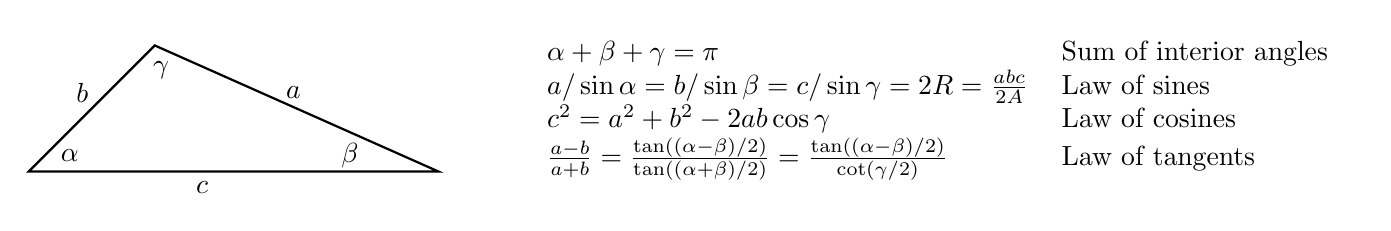
\begin{tikzpicture}[thick, scale=0.4]
\draw (0,0)--(13,0)--(4,4)--cycle;
\node at ( 1.3, 0.5) {$\alpha$};
\node at (10.2, 0.5) {$\beta$};
\node at ( 4.2, 3.2) {$\gamma$};
\node at ( 5.5,-0.5) {$c$};
\node at ( 1.7, 2.5) {$b$};
\node at ( 8.4, 2.5) {$a$};
%\node[align=left] at (17,3) {$c^2=a^2+b^2$\\ $b^2=p^2+h^2$ \\ $a^2=q^2+h^2$};
\node[align=left] at (29,2) 
{
\begin{tabular}{l l}
  $\alpha + \beta + \gamma = \pi$                       & Sum of interior angles \\
  $a / \sin \alpha = b / \sin \beta 
    = c / \sin \gamma 
    = 2R = \frac{abc}{2 A}$                             & Law of sines \\  
  $c^2 = a^2 + b^2 - 2ab \cos \gamma$                   & Law of cosines \\
  $\frac{a-b}{a+b} 
   = \frac{\tan((\alpha-\beta)/2)}{\tan ((\alpha+\beta)/2)} 
   = \frac{\tan((\alpha-\beta)/2)}{\cot (\gamma/2)}$
                                                        & Law of tangents \\
\end{tabular}
};
\end{tikzpicture}
\medskip

%\medskip
%\begin{tabular}{l l}
%  $\alpha + \beta + \gamma = \pi$                       & Sum of interior angles \\
%  $a / \sin \alpha = b / \sin \beta 
%    = c / \sin \gamma 
%    = 2R = \frac{abc}{2 A}$                             & Law of sines \\  
%  $c^2 = a^2 + b^2 - 2ab \cos \gamma$                   & Law of cosines \\
%  $\frac{a-b}{a+b} 
%   = \frac{\tan((\alpha-\beta)/2)}{\tan ((\alpha+\beta)/2)} 
%   = \frac{\tan((\alpha-\beta)/2)}{\cot (\gamma/2)}$
%                                                        & Law of tangents \\
%\end{tabular}
%\medskip
% maybe try to draw a triangle next to to the table showing all the quantities...without taking any more vertical space ...it doesn't seem to work - maybe do it in the same way as with the right triangle - include the formulas into the tikz picture - use two columns of text
% OK - done...the commented tabular environment is now inside the tikzpicture


where the quantities $R, A$ appear. These and others can be computed via:

\medskip
\begin{tabular}{l l}
 $s = (a+b+c)/2$                       & Semiperimeter, half of the perimeter \\
 $A = \sqrt{(s-a)(s-b)(s-c) s} = r s$  & Area (via Heron's formula) \\
 $r = \sqrt{(s-a)(s-b)(s-c)/s} = A/s$  & Radius of inscribed circle \\  
 $R = (abc)/ A$                        & Radius of circumscribed circle \\
 $r = \frac{s-a}{\cot(\alpha/2)}
    = \frac{s-b}{\cot(\beta/2)}
    = \frac{s-c}{\cot(\gamma/2)}$      & Law of cotangents\\
\end{tabular}
\medskip


\paragraph{More Formulas} $ $ \newline
% For some reason, we need this "$ $ \newline" nonsense to convince LaTeX to put the tabular
% on a new line

%\medskip
\begin{tabular}{l l}
 $\sin(\gamma / 2) = \sqrt{ (s-a)(s-b) / (a b)  }$      & Half-angle formula for sine \\
 $\cos(\gamma / 2) = \sqrt{ s(s-c) / (a b)  }$          & Half-angle formula for cosine \\
 $\tan( \gamma) = \frac{c \sin \alpha}{b - c \cos \alpha}
              = \frac{c \sin \beta} {a - c \cos \beta}$ & Tangent formula  \\
 $\frac{a-b}{c} 
   = \frac{\sin( (\alpha - \beta)/2) } { \sin( (\alpha + \beta)/2) }
   = \frac{\sin( (\alpha - \beta)/2) } { \cos( \gamma/2) } $
                                                        & Mollweide formula for sine \\
 $\frac{a+b}{c} 
 = \frac{\cos( (\alpha - \beta)/2) } { \cos( (\alpha + \beta)/2) }
 = \frac{\cos( (\alpha - \beta)/2) } { \sin( \gamma/2) } $
                                                        & Mollweide formula for cosine \\
 $c = a \cos \beta + b \cos \alpha$                     & Projection theorem \\  
 $H_a = b \sin \gamma = c \sin \beta$                   & Height above side $a$ \\ 
 $A = a H_a / 2$                                        & Area via height \\
 $M_c = \sqrt{2(a^2+b^2) - c^2}/2
      = \sqrt{a^2+b^2 +2ab\cos\gamma}/2$                & Length of median of side $c$ \\
 $B_{\gamma} = (2ab\cos(\gamma/2))/(a+b)
      = \sqrt{ab \; ((a+b)^2-c^2)}/(a+b)$               & Length of angle bisector of $\gamma$
\end{tabular}
\medskip


These are quite a lot of moderately complicated formulas already (you perhaps see now why we really don't want to memorize them) and by symmetry, even more formulas can be obtained by doing the cyclic replacements: $a \rightarrow b \rightarrow c \rightarrow a$, $\alpha \rightarrow \beta \rightarrow \gamma \rightarrow \alpha$. 


\paragraph{More Definitions and Facts}
A couple of terms appeared in the descriptions of the formulas above. They deserve some explanation. The \emph{perimeter} is the total length of all the sides, i.e. the length that you would have to walk if you walk around the triangle. The \emph{semiperimeter} is half of that. The \emph{median} of a side is the line segment that starts from the middle of that side and goes to the vertex that is opposed to that side. All 3 medians meet in a common point which is the \emph{center of gravity} of the triangle. The \emph{angle bisector} is a line segment resulting from drawing a line in between the two triangle sides from a vertex using half of the angle there and extending it until it hits the opposing side. All 3 angle bisectors meet in a common point which is also the \emph{center of the inscribed circle} of the triangle. The \emph{center of the circumscribed circle} is given by the point where \emph{perpendicular line segment bisectors} meet. These are lines starting at the centers of the sides in a direction perpendicular to the respective side (ToDo: is there a formula for their lengths, too? maybe draw triangle with medians, bisectors, inscribed circle, etc. Explain center of gravity as balancing point).

% see Teubner tachenbuch, page 760,764
% https://de.wikipedia.org/wiki/Projektionssatz_(Dreieck)
% todo: law of cotangents, what about centers of the incircle and circumcircle? but maybe that's for analytic geometry because it involves coordinates

% https://en.wikipedia.org/wiki/Semiperimeter
%   "appears frequently enough in formulas for triangles and other figures that it is given a
%   separate name" 
% Is this one of the reasons why pi = tau/2 also appears quite often? pi is the length of
% semiperimeter of a circle. It gives another reason to call pi the semicircle constant.

\subsubsection{Congruence Theorems}
In geometry, two shapes are said to be congruent if they can be brought into full agreement just by means of translations, rotations and reflections - fancy terms for moving, turning and mirroring. It captures the idea that the two shapes are the same, just possibly placed somwhere else in space with a possibly different orientation. There are 5 theorems that state sufficient conditions for two triangles to be congruent. Two triangles are congruent if at least one of the following statements holds true: (SSS) all three sides have matching lengths, (ASA) one side and the two adjacent angles match, (SAS) one angle and the two adjacent sides match, (AAS) two angles and one side match, (SsA) two sides and the angle adjacent to the smaller side match (the lowercase 2nd s is not a typo - it indicates the smaller side). ...ToDo: verify these, especially SsA and give the formulas/algorithms to compute the missing pieces. Explain also similarity (here, also scaling is allowed - its should preserve only distance ratios where congruence preserves distances themselves. I think it also preserves angles)

% on (SsA): https://www.jstor.org/stable/27966706

%https://tutors.com/math-tutors/geometry-help/triangle-congruence-theorems-sss-sas-asa
%https://j-tradition.com/congruence.html


\subsubsection{Right Triangles}
Of special importance are triangles in which one angle is a right angle. These are unsurprisingly and rightfully called right triangles. There can be only one right angle in a non-degenerate triangle because two right angles already sum up to a straight angle, which is also the sum of all 3 angles - so if you attempt to have two right angles, you'll get (in the limit) a degenerate triangle whose 3rd vertex is at infinity with an angle of zero (because they are parallel). By the way, triangles in which two sides have the same length are called \emph{isosceles} and those where all three sides are equal are called \emph{equilateral}. But this is just more jargon and not super important. The right triangles are the mathematically important ones. Pictured below is a right triangle with sides $a,b,c$ that is split into two further right triangles by a drawing a perpendicular from the top vertex to the base side $c$. The height of the triangle is denoted by $h$. Next to it are some relevant formulas that hold in such a situation.

\medskip
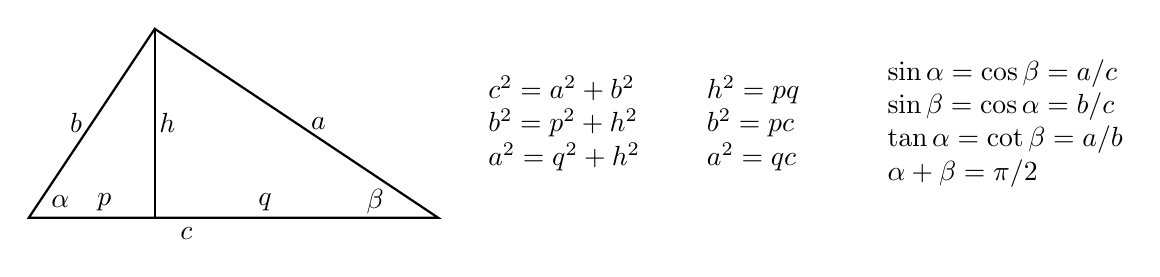
\begin{tikzpicture}[thick, scale=0.4]
\draw (0,0)--(13,0)--(4,6)--cycle;
\draw (4,6)--(4,0);
\node at (1.0, 0.5) {$\alpha$};
\node at (2.4, 0.5) {$p$};
\node at (7.5, 0.5) {$q$};
\node at (11.0, 0.5) {$\beta$};
\node at (5.0,-0.5) {$c$};
\node at (1.5,3.0)  {$b$};
\node at (9.2,3.0)  {$a$};
\node at (4.4,3.0)  {$h$};
\node[align=left] at (17,3) {$c^2=a^2+b^2$\\ $b^2=p^2+h^2$ \\ $a^2=q^2+h^2$};
\node[align=left] at (23,3) {$h^2 = p q$ \\ $b^2 = p c$ \\ $a^2 = q c$};
\node[align=left] at (31,3) {$\sin \alpha = \cos \beta = a/c$ \\ 
   $\sin \beta  = \cos \alpha = b/c$ \\ 
   $\tan \alpha = \cot \beta  = a/b$ \\ 
   $\alpha + \beta = \pi/2$};
\end{tikzpicture}
\medskip
% see Teubner Taschenbuch, page 761
% see at around 19:40 - Inverser Satz des Pythagoras: 1/a^2 + 1/b^2 = 1/h^2
% https://www.youtube.com/watch?v=od9lUVypXrQ


The $a^2 + b^2 = c^2$ relation is the famous theorem of Pythagoras which is a special case of the law of cosines when the angle $\gamma$ is a right angle in which case the cosine term vanishes ($\gamma$ is not shown - it's the angle opposite to side $c$). The two equations below are the same theorem applied to the sub-triangles. In the middle column are Euclid's altitude theorem (aka height theorem) and below are his theorems of sides. In the right column are some angle relations. [ToDo:verify everything, especially the $\cot \beta$ relation - it's just a guess from symmetry, maybe add also the converse relation for b/a] 

% https://tex.stackexchange.com/questions/29233/tikz-adding-text


%\begin{tikzpicture}[thick, scale=0.75]
%\draw (0,0) coordinate[label=below:$A$] (a) --
%      (4,0) coordinate[label=below:$B$] (b) --
%      (4,3) coordinate[label=above:$C$] (c) -- cycle;
%\end{tikzpicture}

%\include{Tikz/RightTriangle_4_3} % doesn't work - includes can't be nested - that sucks!!!

\subsubsection{More Triangle Facts}
% https://texample.net/tikz/examples/morleys-triangle/ trisectors always from an equilateral triangle

% there is a circle going through all of the 3 vertices - this is called the circumcircle and its center is called the crucumcentre

% each triangle has 3 "altitudes" (lines from one vertex going down orthogonally to its opposing side). They meet in a common point called the "Orthocentre"
% see: https://www.youtube.com/watch?v=ZrjarkXS0Fo

\subsection{Quadrilaterals}
% rant about why they are not called quadrangles or triangles not trilaterals

% see: https://www.youtube.com/watch?v=ZrjarkXS0Fo at 6:00
% -opposite angles in a cyclic quadrilateral sum to 180°  -and vice versa: if two opposite angles in a quadrilateral sum to 180, then the quadrilateral is cyclic (meaning that its 4 vertices lie on a circle) ..shouldn't that be called "circular" rather than "cyclic"

% Ptolemy’s Theorem and the Almagest: we just found the best visual proof in 2000 years
% https://www.youtube.com/watch?v=rr1fzjvqztY
% In any cyclic quadrilateral (i.e. qudrilatral inscribed in a circle). Label 2 opposite sides A,a and the tow other opposite sides B,b and the two diagonals C,c. Then: A*a + B*b = C*c. If the quadrilateral is a rectangle, we recover Pythogoras's theorem a special case.

% https://en.wikipedia.org/wiki/Semiperimeter#For_quadrilaterals

\subsection{Polygons}
% sums of interior and exterior angles, regular polygons, convexity, self-intersection


% Gauß' geniale Methode zur Flächenberechnung von Vielecken
% https://www.youtube.com/watch?v=EUAH2rSJ9Ao
% -"Schnürsenkelmethode"
% https://de.wikipedia.org/wiki/Gau%C3%9Fsche_Trapezformel
% https://en.wikipedia.org/wiki/Shoelace_formula


\subsection{Circles}

% introduce circle as 
% (1) limiting case for a regular polygon as the number of sides grows.
% (2) locus of all points at a fixed distance from some given center

% https://www.youtube.com/watch?v=rr1fzjvqztY
% 6:20: start with any chord of the circle. from the ends of the chord, draw lines that meet at the circle. all pairs of such lines will meet in the same angle at the circle
% if you also draw lines to the center of the circle, the meeting angle at the center is twice that of the meeting angle at the boundary
% when the chord goes through the center, the meeting angles at the circle's boudary are 90° (Thales theorem)

% https://en.wikipedia.org/wiki/N-sphere#Spherical_coordinates


%\subsection{Conic Sections}

%\subsection{General Shapes}
% by 2D shape, we usually mean something deescribed by a closed, non self-intersecting curve
% ..but we have already seen more general things: polygons that self-intesect, curves that 
% aren't closed (hyperbolas). We usually think of a shape 2D as something that has an area.
% That makes sense only for closed curves. When they self-intersect, we can still make sense 
% of it but the notion of area becomes a bit ambiguous - should some parts of the figure 
% count as negative area? Maybe based on the direction of winding of the edges around that
% sub-area? Consider a figure 8

\subsection{Geometric Derivations}
You may wonder, how all these formulas were derived geometrically or how one would go about deriving a formula geometrically at all. The process starts with a couple of points, lines or line segments and maybe circles and then makes use of the Euclidean axioms: we may pick any pair of points and draw a line between them, we may extend lines as we see fit, we may draw a circle centered at one of our points with a radius given by the distance between any pair of our points. In such a construction, we may then identify angles that must be equal to each other by the rules of corresponding, opposite, alternating or consecutive angles. We may identify sums of angles that must sum up to a right, straight or full angle. We may identify line segments or distance ratios that must be equal to each other. We may identify shapes that are congruent or similar to one another. All of that will give us equations. The "identification" of known geometric situations in itself requires two steps: recognition (usually by eye - like: "hey, these two triangles look similar!") and proof (usually by making geometric arguments based on known theorems - "like: they must indeed always be similar because of such and such theorem"). What exactly to do in a given situation to find such equations is a highly creative process. Look up "Dandelin Spheres" or watch 3blue1brown's "Why slicing a cone gives an ellipse" video for a nice example of such a geometric proof. [TODO: include a reference] A much simpler example is the proof that the sum of all angles in a triangle must be a straight angle...

% https://www.youtube.com/watch?v=pQa_tWZmlGs
% https://en.wikipedia.org/wiki/Dandelin_spheres

ToDo: draw the picture that shows that the angles in a triangle must sum to 180


% Explain that it is importnat to not jump to conclusions from a particluar drawing. In geometry, there often are a lot of different cases and configurations to consider and the drawn one is usually just one of them. We must make sure to really take into account all possible configurations.


% The AI that solved IMO Geometry Problems | Guest video by ‪@Aleph0‬
% https://www.youtube.com/watch?v=4NlrfOl0l8U
% -Explains computer algorithms (with and without AI) that solve geometry problems
% -Explains that geometrioc derivations often involve "auxiliary constructions" - drawing in lines,
%  circles, etc. that are not there already
% -Coming upt with such auxiliary constructions is hard - the search space of possible constructions
%  is infinite


\subsection{3D Geometry}

% angles in 3D, solid angles

\subsubsection{Platonic Solids}
% all faces, sides and angles are the same
% tetrathedron, cube, ...

\subsubsection{Polyhedra}
% Euler's formula, generalization to nD: polytopes (I think)

\subsubsection{Solids of Revolution}
% sphere (revolve a half-circle), cylinder (revolve a rectangle), cone (revolve a 
% right triangle)


\begin{comment}
	
Maybe explain why we say triangles and quadrilaterals but not, more consistently, either triangles and quadrangles or trilaterals and quadrilaterals. One suffix-term focuses on the angles, the other on the sides - I think

https://texample.net/tikz/examples/area/geometry/
http://www.tikzedt.org/

https://github.com/walmes/Tikz  examples mainly for statistics

-center circumscribed circle: intersection of medians
-center of inscribed circle: intersection of angle bisectors

https://en.wikipedia.org/wiki/Median_(geometry)
https://de.wikipedia.org/wiki/Seitenhalbierende

https://mathworld.wolfram.com/AngleBisector.html
https://en.wikipedia.org/wiki/Angle_bisector_theorem
https://en.wikipedia.org/wiki/Bisection#Triangle
https://de.wikipedia.org/wiki/Winkelhalbierende

https://mathworld.wolfram.com/PerpendicularBisector.html
https://en.wikipedia.org/wiki/Bisection#Perpendicular_line_segment_bisector
https://de.wikipedia.org/wiki/Mittelsenkrechte

https://en.wikipedia.org/wiki/Incircle_and_excircles_of_a_triangle

https://en.wikipedia.org/wiki/Mollweide%27s_formula

https://en.wikipedia.org/wiki/Law_of_cotangents

https://en.wikipedia.org/wiki/Circle

-thales' theorem

-rename file to Geo_Elementary

-plot a drawing of a triangle with vertices A,B,C, sides a,b,c and angles alpha, beta, gamma
-give a bunch of formulas that hold for all triangles
-the plot some special triangles (right, isosceles, etc.) and give the formulas specific to them
-mention non-Euclidean trigonometry, espeically spherical...maybe give the formulas for those
triangles, too - or maybe refer to some ressource

-give formulas for volumes of 3D shapes

https://en.wikipedia.org/wiki/Trigonometry

Weitz: Elementargeometrie (Vorkurs Mathematik)
https://www.youtube.com/watch?v=cMuoFr4DvDo

Weitz: Überblick Elementargeometrie: Winkel, Satz des Pythagoras, Sinus, Kosinus, etc.
https://www.youtube.com/watch?v=zVLFfgg7f98&list=PLb0zKSynM2PBYzz6l37rWH3B_n_7P40QP&index=167

How many lines go through 4 given lines in 3D?
https://www.youtube.com/watch?v=F5d8fUXf7d8
-6:40 Galucci's Theorem: 3 skew lines in 3D always define a ruling of either hyperboloid 
 or (in exceptional cases when all 3 lines are parallel to the same plane) a hyperbolic 
 paraboloid (see also: ruled surface). 
-A hyperboloid has two different rulings. A line from one such ruling intersects all lines of the
 other ruling. 
-This implies that for 3 given lines in 3D, there are infinitely many lines that intersect all 3.
-For 4 given lines on 3D, there are 4 cases: 
 1: the 4th line does not intersect the hyperboloid -> no line exists that intersects all 4
 2: the 4th line is tangent to the hyperboloid -> one line intersects all 4
 3: the 4th line pokes through the hyperboloid -> two lines intersect all 4
 4: the 4th lines lies on the same ruling of the hyperboloid -> infinitely many lines intersect 
    all 4 (namely, those on the opposite ruling)
-This is a topic of enumerative geometry and Schubert Calculus

the forgotten 3 dimensional Pythagorean theorem.
https://www.youtube.com/watch?v=vcnQ0GR4IPI
https://en.wikipedia.org/wiki/De_Gua%27s_theorem

Divine high PHI: The power of AB=A+B (Mathologer masterclass)
https://www.youtube.com/watch?v=cCXRUHUgvLI
at 6:40 - Ptolemys theorem - generalization of Pythagoras theorem

-Hint at non-Eulcidean geometries: 
 -straight lines don't exist anymore - we need to use geodesics instead
 -spherical: angle sum in triangles is > pi, ratio of circumfence to radis in circle is
  < pi, 
 -hyperbolic:
 -This will be picked up in more detail in the context of differential geometry


Red or Green: Which is larger? (Guess before you watch)
https://www.youtube.com/watch?v=xKQuEREy5fY


\end{comment}
\section{Differential Geometry}
In algebraic geometry, we considered zero sets of systems of polynomial equations. Under certain circumstances, these zero sets define a manifold and sometimes, we could find a parametric representation of such a manifold, i.e. a formula, that takes as input one or more independent parameters and spits out a point on the manifold as output. Differential geometry (DG) typically takes a parametric representation, i.e. a vector valued function of possibly multiple arguments, of such a manifold as a starting point. Since we will need to take work with (partial) derivatives of such a parametric representation, we will assume that all the functions are differentiable sufficiently often.

\medskip
DG can be roughly split into "classical" or "elementary" DG and "modern" DG. The former deals with curves in the 2D plane and with curves or surfaces in 3D space and is typically expressed in (a subset of) the language of vector calculus. The latter deals with the completely general case of $kD$ manifolds in $nD$ space where $k \leq n$ and is typically expressed in (a subset of) the language of differential forms (aka exterior calculus) and/or tensor calculus. Important applications of classical DG are in computer graphics, modern DG features prominently in general relativity.

\medskip
A very important, maybe the most important, concept in DG is the idea of curvature.

% curves vs surfaces vs general manifolds, intrisic vs extrinsic

...tbc...



\begin{comment}
	
In algebraic geometry, we deal with a manifold that is defined by an implicit equation of the form f(x,y) = 0 in 2D or f(x,y,z) = 0 in 3D or a system of such equations like f(x,y,z) = 0, g(x,y,z) = 0 in 3D. The equations are assumed to be polynomials but (I guess) the general ideas can be generalized to arbitrary equations. The manifold is typically of a dimensionality given by the dimensionality of the embedding space minus the number of equations (verify!). When I say "typically", I mean that there may be other cases but these can be considered as somehow being degenerate edge cases (verify!). For example, if we have have 1 equation in 3 variables, we normally get a 2D manifold, i.e. a surface in 3D space. 

In differential geometry, we also deal with manifolds but here, the manifolds are not defined via an implicit equation but rather by a set of parametric equations. We can imagine the parametrization to define a map of the manifold. We may have different parametrizations (i.e. maps or charts or patches) for different regions. The totality of all these maps (i.e. the set of all the maps) is called an atlas. Ideally, the maps should cover the whole manifold. Different maps may overlap with respect to the region that they cover. If they do overlap, they should agree in the regions of overlap. ...tbc...

In some sense, algebraic geometry is simpler than differential geometry because it just involves solving algebraic equations. Differential geometry, on the other hand, uses a lot of calculus which is usually considered to be a more advanced math topic than algebra. But in some other ways, differential geometry might also be considered easier that algebraic geometry because in DG we have the luxury of getting a parametrization of our manifold handed to us on a silver plate. Such a parametrization is for many purposes a much more convenient description of the manifold than the unwieldy implicit equation that AG gives us. One could actually say that the availability of the parametrization \emph{enables} us to make use of a lot of calculus that would unavailable otherwise.

differential: local properties such as curvature, metric tensor, gradient, tangential plane/space
algebraic: global properties such as number of holes, orientability, number of stationary points, number of
 self-intersections, winding number

https://mathworld.wolfram.com/Atlas.html
https://en.wikipedia.org/wiki/Atlas_(topology)#Charts

ToDo:
-There are at least 2 ways of defining a surface in 3D: 
 -parametrically as x(u,v), y(u,v), z(u,v) - that's the DG approach
 -implicitly as F(x,y,z) = 0 - that's the AG approach
-An explicit form z = f(x,y) can be seen a special case of both:
 parametric: x(u,v) = u, y(u,v) = v, z(u,v) = f(u,v)
 implicit:   F(x, y, f(x,y)) = 0
-Explain, how we can get a local parametrization from an implicit equation using
 partial derivatives...I'm not sure, if that's possible but I think, it should be.
 See:
 https://tutorial.math.lamar.edu/classes/calciii/parametricsurfaces.aspx
-Maybe we could also try to convert locally to an explicit form. It would become locally
 a 1D root-finding problem of F(x,y,z) = 0. Here, x,y are plugged in and can be seen as 
 parameters and we want to find z.
-Explain how we may get an implicit form from a given parametrization
-Sochi's book says that DG is more concerned with local features of the manifolds whereas
 AG is more about global features.
-I think, the fundamental local feature in DG is the metric tensor. Most other quantities of
 interest can be derived from it. In the case of surfaces, the metric tensor is just a 2x2 
 matrix. It can be computed from the extrinsic description of the surface via its 
 parametrization but one often just assumes it to be *somehow* given without caring much about 
 the how. It is an intrinsic feature of the manifold that can also be measured from an observer 
 who lives inside the manifold (Like A. Square living in flatland). Derived quantities are
 the different forms of curvature (except geodesic curvature which is an extrinsic property), 
 the Christoffel symbols, etc.
-Global features are things like the number of stationary points, orientability, presence or 
 absence of self-intersections, topological features such as the genus, ...

-Maybe use a circle of radius 5 as example curve and represent it 
 parametrically: c(t) = (5 cos(t), 5 sin(t))
 implicitly:  x^2 + y^2 - 25 = 0
 explicitly: y = +- sqrt(25 - x^2)
 and compute the tangent vector at a point (say (4,3)) via all 3 representations. Investigate, 
 how we can, from a given implicit equation and a point on the curve, compute coordinates of 
 another (infinitesimally) nearby point. Parametric and explicit representations can be used
 straightforwardly to "generate points" - but how can the implicit equation be used for that?
 1: by considering it a root-finding problem, 2: by assuming that we have a point given and
 somehow obtain a nearby point? ..which we may or may not refine using a root-finder?

%An Amazing Theorem for Tangents (Fabricius-Bjerre Theorem)
%https://www.youtube.com/watch?v=7_UclB2dB0o

Differential Geometry: The Intrinsic Point of View #SoME3
https://www.youtube.com/watch?v=jWoyBlIXVd8
-Gaussian curvature, being the product of two extrinsic quantities (namely, the two principal
 curvatures), turns out to be an intrinsic property. That's what Gauss found remarkable, according
 to this video. The "Theorema Egregium" itself is of a more quantitative nature, though.
-The Riemann curvature tensor is the nD generalization of Gaussian curvature.


https://en.wikipedia.org/wiki/Lie_derivative

How mathematicians describe curvature of surfaces
https://www.youtube.com/watch?v=UYiAlYlSwBo

What is Differential Geometry?
https://www.youtube.com/playlist?list=PLXo8Tdaw0czOWyRD-esa6mNajlPZnjHQs


Lisa Piccirillo: Exotic Phenomena in dimension 4
https://www.youtube.com/watch?v=BXwALAkPubc

How to Get to Manifolds Naturally
https://www.youtube.com/watch?v=lEX4kSB5CAI

How to do Calculus on an Abstract Manifold
https://www.youtube.com/watch?v=pNlcQ0Tx4qs


the geometry of the third derivative
https://www.youtube.com/watch?v=h4kGXlKz5GI



https://www.youtube.com/watch?v=o8swNKLHDzo  How to describe Curvature?
-5:44: for a triangular region:  sum-of-angles - 180° = integral over Gaussian curvature
 ...but I guess the 180° must be re-expressen in radians?
-7:02: sufaces with zero mean curvature are minimal surfaces
 Q: is the converese also true?


Differential Geometry in Under 15 Minutes
https://www.youtube.com/watch?v=oH0XZfnAbxQ
-Nice overview - also explains Stokes' Theorem in terms of differential forms

Why Distances Depend on the Geometry You Live In
https://www.youtube.com/watch?v=5qAvXdBTISo

The Core of Differential Forms
https://www.youtube.com/watch?v=DOPwupMCcUs
-A 1-form is a generalization of a directional derivative. It takes a vector as input and
 produces a scalar as output

How to Describe an Entire Space with a Matrix
https://www.youtube.com/watch?v=bt7Msd1b5VA
-about the Ricci curvature tensor (a symmetric rank 2 tensor)
-it quantitfies how geodesics bend together or drift apart 
-this can also be understood in terms of how hypervolumes expand when we move outward from a point
-nD generalization of the 2D concept of Gaussian curvature (?) ...or rather maybe a generalization
 of the principal curvatures?
-defined as contraction of Riemann curvature tensor (rank 4 tensor)
-

But what are manifolds, anyway? (Explained at 5 levels of difficulty)
https://www.youtube.com/watch?v=OdWaYWtrZI4
-Very nice and intuitive explanation

Manifolds
https://www.youtube.com/watch?v=aDzX6rsALy0


\end{comment}

\chapter{Functional Analysis}
Functional analysis studies operations that take a function as input. As output, these operations may produce another function in which case they are called operators, or just a simple number in which case they are called functionals. Some simple examples of operators, operating on a function $f$, are: take the derivative of $f$, take an antiderivative, multiply the input function $f$ by some (fixed) other function $g$. An example for a functional $F$ that just produces a number as output would be to take the definite integral of $f$ over some given interval $(a,b)$. An even simpler, nonetheless practically very relevant, example of a functional $F(f)$ of a function $f = f(x)$ is to just extract the value of $f$ at a given $x$, for example at $x=0$, so we would just have $F(f) = f(0)$. In any case, we are one level higher up the ladder: we are now talking about functions-of-functions, so to speak. Especially in computer science, such higher level function-like objects are also sometimes called functors. 

\paragraph{}
Functional analysis plays an important role in the study of differential equations. An ordinary differential equation (ODE), for example, may take a "driving function" as input (i.e. as right-hand-side, inhomogeneity) and produce as output a solution function which can be interpreted as the "response" of a system for the given input function. In such a context, we may in practice have to deal with driving functions that are not necessarily differentiable or even continuous - but when dealing with differential equations, we often really need to be able to take derivatives. That's one reason why a generalized notion of function-like objects, called distributions, is introduced. For these distributions, we have a notion of differentiation that is always applicable - even in the case of discontinuous functions. This notion will help us to find solutions to ODEs even for such discontinuous driving functions which we otherwise just couldn't handle properly. A strange object, called the Dirac delta-distribution $\delta(x)$, will play an important role in this context. It can be thought of as a "function" that is zero everywhere except at $x=0$ where it is infinite in such a way that the integral over any interval that includes $x=0$ equals unity. It represents an inifinitely narrow impulse of unit energy concentrated at $x=0$. No classical function behaves in such a bizarre way. If we know the response of a linear ODE to such an impulse, we can compute the response to any driving function as superposition of such impulse-responses. This superposition will be a continuous one, given by an integral, called the convolution integral.

\paragraph{}
In the context of boundary value problems and/or partial differential equations (PDEs), this notion of an impulse response will be generalized to what is called a Green's funcion...tbc...

\paragraph{}
An important type of operators are integral operators, prominent examples of which are given by the Fourier- and Laplace transform. These transforms take functions from one space (the time domain) to another (the frequency domain) and in this new space, the complicated process of convolution can be replaced by a simple pointwise multiplication. Moreover, the frequency domain is more intuitive for human interpretation - we may identify perceptually important features of signals often more easily in the frequency domain, especially in the case of audio signals.
..tbc...

\paragraph{}
In multivariable calculus, we have already seen concepts from linear algebra and calculus merge to produce new, hybrid objects like vectors and matrices of partial derivatives like the gradient vector and the Jacobian and Hessian matrices. In functional analysis, these two important fields of mathematics also come together, but this time in a very different way: Certain sets of functions will be equipped with some more structure on the set so as to form vector spaces. This additional structure may contain linear-algebra'ish things like norms of functions, scalar products between functions, linear mappings of functions to other functions, etc. These mappings often involve calculusy things like taking derivatives or integrals. These function spaces, i.e. vector spaces whose elements/vectors are functions, will often be infinite-dimensional which is a qualitative difference to the finite-dimensional vector spaces we have seen before. Nonetheless, we'll see a lot of analogies. Let's get started!

\begin{comment}


-integral transforms (fourier- and laplace trafo)
-greens-functions
-calculus of variations
-operators: eigenvalues, eigenfunctions


\end{comment}
\section{Function Spaces}
Recall from linear algebra the general definition of a vector space as a set of elements, called vectors, that can be added together to give another vector or multiplied by a scalar (i.e. a number) to give another vector. Now notice that we can do these two things with functions just the same: adding two functions pointwise gives a perfectly valid other function and multiplying a function by a number also gives another bona fide function. It can be easily verified that all the required vector-space rules such as associativity, commutativity, distributivity, neutral elements, etc. are satisfied for these operations, when applied to functions. That means, we can actually view the set of all real-valued functions $f: \mathbb{R \rightarrow R}$ as a vector space! This vector space, however, has a fundamentally different nature than those we have seen before. In order to uniquely determine a function $f$, we will have to say what its function value will be for any given input value $x$. If the domain of the function is the whole real number line (or even just a finite interval of it), that means, we must prescribe (uncountably) infinitely many function values, so the dimensionality of the space of all functions that map real numbers to real numbers is apparently also (uncountably) infinite. We will also encounter subspaces of this huge space whose dimensionality will be only countably infinite or even just finite.

\subsection{Scalar Products}
In the $N$-dimensional vector space $\mathbb{R}^N$, the standard scalar product of two vectors $\mathbf{u,v}$ was defined as the sum over the element-wise products:
\begin{equation}
 \langle \mathbf{u,v} \rangle = \sum_{i=1}^{N} u_i v_i
\end{equation}
That motivates the definition of the scalar product of two real-valued functions $f,g$, both defined on some interval $(a,b)$, by analogy as:
\begin{equation}
 \langle f,g \rangle = \int_a^b f(x) g(x) \; dx
\end{equation}
This is one possible definition of a scalar product on a space of functions and it is in fact the one that is most often used, but there are some other variations that should be mentioned, too. ...
% introduce the general from with a weight and maybe also the complex form, maybe also with a positive definite kernel, what about the integration limits, there are also scalar products involving derivatives

\subsection{Norms and Distances}
In $\mathbb{R}^N$, the Euclidean norm of a vector was defined as the square root of the scalar product of the vector with itself. We can define a norm for functions in a completely analogous way. However, we don't necessarily need a scalar product to define a norm. Another way to define a norm would be to just take the maximum value of the function within a given interval. ...
% L_p-norm, maximum-norm, norms induced by a scalar product, distances (norms of differences)

\subsection{Special Function Spaces}
Often we are not interested in the vast and unstructured set of all possible real functions but only in a subset of it, i.e. in a set of functions that meet some additional criteria. We may, for example, demand that the functions have to be continuous, differentiable, (square-)integrable, bounded, periodic, monotonic, symmetric, etc. It turns out that many of these subsets are actually also subspaces in the sense that addition of two such functions or multiplication of one of them by scalar will always give a new function that also belongs to the set. Some of these specific function spaces are important enough that they have been given special names, so we shall now familiarize ourselves with this terminology.

\subsubsection{Continuity and Differentiability}
One way to categorize functions is by considering, how smooth they are. Does a function $f$ have spikes, jumps, corners, etc? That idea is captured by the number of continuous derivatives that a function has. If a function is $k$ times continuously differentiable, then it is said to be in the class $C^k$. If a function is just itself continuous but has a discontinuous first derivative, it is in the class $C^0$ but not in the class $C^1$. An example of such a $C^0$ but not $C^1$ function would be the absolute value $f(x) = |x|$. In general, the classes with lower $k$ are less restrictive, i.e. allow more functions. But the classification is meant in an inclusive sense, i.e. a function that is in $C^k$ is automatically also in $C^j$ if $j < k$. If a function can be differentiated $k+1$ times, it means that the $k$-th derivative is not only continuous but even differentiable which is a stronger requirement. That means, a function that can be differentiated $k+1$ times is automatically at least in $C^k$. If a function can be differentiated infinitely often, it is said to be in the class $C^\infty$. Such functions are also called \emph{smooth}. If, in addition to be infinitely differentiable, it also has a convergent Taylor series at every point of its domain, it said to be in $C^\omega$ and also called \emph{analytic}\footnote{The letter $\omega$ is also used in other areas of math (ordinal numbers, nonstandard analysis) to denote "infinity". I'm not sure, if that usage there is related but to be honest, I can't see how. It seems like the $\omega$ from ordinal numbers would mean exactly the same thing as the $\infty$ symbol as it is used here. So maybe drawing a connection would be a bit hasty.}. Analytic functions are in some sense even nicer than just smooth ones.

%...TODO: define $C^k$ spaces including $C^\infty$ and $C^\omega$

% Bump functions are in  $C^\infty$ but not in $C^\omega$. Explain why!

% https://en.wikipedia.org/wiki/Smoothness
% https://mathworld.wolfram.com/C-kFunction.html

\subsubsection{Integrability} Functions can also be categorized according to their integrability. By analogy with the classification based on differentiability, you might guess that we consider repeated integration of a function. But that's not how it works. Instead, we consider the integral of the $p$-th power of the absolute value of the function. For example, for functions $f: \mathbb{R} \rightarrow \mathbb{R}$, we may consider the integral of the absolute value of $f$ over the whole domain: $\int_{-\infty}^{+\infty} |f(x)| \; dx$ and classify those functions for which this integral is finite as belonging to the class of \emph{absolutely integrable} functions over the real numbers. Next, we may introduce an exponent $p$ to whose power we raise the absolute value and look at $\int_{-\infty}^{+\infty} |f(x)|^p \; dx$ and requiring that integral to be finite. For the special case $p=2$, we call the class of functions \emph{square integrable} and for general $p$, we call the functions \emph{$p$-th power integrable}. Generalizing further, we may consider functions $f: \mathbb{R}^n \rightarrow \mathbb{R}$ and look at $\int_{\mathbb{R}^n} |f(x_1, x_2,\ldots,x_n)|^p \; dx_1 dx_2 \ldots dx_n$ and requiring that integral to be finite. Generalizing even further, we may consider functions from any set $S$ for which a measure $\mu$ is defined into the real numbers\footnote{I guess, it could be generalized even further to allow the codomain be any set $T$ on which a suitable absolute value function is defined. $T =\mathbb{R}$ or $T = \mathbb{C}$ are two obvious choices.} $\mathbb{R}$ such that $f: S \rightarrow \mathbb{R}$ and requiring $\int_S |f|^p \; d \mu $ to be finite. This integral is apparently meant to be understood as a Lebesgue integral - so we require that the $p$-th power of the absolute value of $f$ must be Lebesgue integrable and the integral must be finite. We denote this set of functions by $\mathcal{L}^p(S,\mu)$ and call it the set of \emph{measurable functions} [VERIFY!]

%When talking about measures, it is clear


%any set of objects $T$ on which an absolute value is defined (such as $T =\mathbb{R}$ or $T = \mathbb{C}$)

% The normed vector space ( L p ( S , μ ) , ‖ ⋅ ‖ p ) {\displaystyle \left(L^{p}(S,\mu ),\|\cdot \|_{p}\right)} is called L p L^{p} space or the Lebesgue space of p p-th power integrable functions

%This idea could be generalized to functions $f: \mathbb{R}^n \rightarrow \mathbb{R}$ by considering $\int_{\mathbb{R}^n} |f(x_1, x_2,\ldots,x_n)|^p \; dx_1 dx_2 \ldots dx_n$ and requiring that integral to be finite.

%That is, for some given $f$, we consider the integral $\int_S |f|^p \; d \mu$ where $S$ is some set on which $f$ is defined (i.e. a subset of the domain of $f$) and $\mu$ is some measure that is defined on $S$ [VERIFY].

% https://en.wikipedia.org/wiki/Lp_space#Lp_spaces_and_Lebesgue_integrals

%\begin{equation}
%\int_S |f|^p \; d \mu
%\end{equation}

%Rather than considering repeated integration (as we did in the case), we consider

%TODO: define $L^p$ spaces named after Lebesgue, explain $\mathcal{L}^p, \ell^p$

% https://en.wikipedia.org/wiki/Lp_space#Lp_spaces_and_Lebesgue_integrals

% https://en.wikipedia.org/wiki/Lp_space
% https://en.wikipedia.org/wiki/Absolutely_integrable_function
% https://en.wikipedia.org/wiki/Square-integrable_function
% https://mathworld.wolfram.com/SquareIntegrable.html

% https://de.wikipedia.org/wiki/Lp-Raum

% https://en.wikipedia.org/wiki/Measurable_function
% https://mathworld.wolfram.com/MeasurableFunction.html


\subsubsection{Normed Function Spaces}
Let's go back the expression $\int_{-\infty}^{+\infty} |f(x)|^p \; dx$ that defines the class of $p$-th power integrable functions $f: \mathbb{R} \rightarrow \mathbb{R}$ by the requirement that this integral must be finite. So far, we really only looked at the cases $p=1$ and $p=2$. We initially intended to let $p$ be a positive natural number but we now want to widen our perspective to allow real $p \geq 1$ and even allow for $p = \infty$. In order to get nice behavior when we let $p$ go to infinity, we will now look at the expression $(\int_{-\infty}^{+\infty} |f(x)|^p \; dx)^{1/p}$. As long as we were just concerned with the finiteness of the integral and $p$ was assumed to be a finite positive number, it didn't really matter whether or not we do the $(\ldots)^{1/p}$ step at the end. But for what we want to do now, namely defining a norm that is still meaningful when $p \rightarrow \infty$, we need this additional reciprocal exponent\footnote{At least, I think this is the reason why we formerly left out the $p$-th root. Consider what happens to the integral expression when $p \rightarrow \infty$: for $|f| < 1$ the integrand will go to zero and for $|f| > 1$ the integrand will go to infinity. It appears like taking the $p$-th root after integration tames this behavior and we get a meaningful limit when $p \rightarrow \infty$.}. We define the $p$-norm of a function $f: S \rightarrow \mathbb{R}$ as
\begin{equation}
 \norm{f}_p = \left( \int_S |f|^p \; d\mu \right)^{1/p}
\end{equation}


 ...TBC...TODO: introduce $p$-norm and $L^p$ spaces as space of equivalence classes of functions from an $\mathcal{L}^p$ space

% https://en.wikipedia.org/wiki/Norm_(mathematics)#p-norm

% https://web.archive.org/web/20201024063542/http://faculty.bard.edu/belk/math461/LpFunctions.pdf

\paragraph{Banach Space}

\paragraph{Hilbert Space}

% https://en.wikipedia.org/wiki/Lp_space#Special_cases
% L^2 is the only Hilber space among the L^p spaces

\paragraph{Sobolev Space}


%\subsubsection{Analytic Functions}
% Smooth Functions, Differentiable Functions
%\subsubsection{Square Integrable Functions}
% finite support

%\subsubsection{Polynomials}
% powers, power series, orthogonal sets of polynomials (Legendre, Chebychev, etc.)

%\subsubsection{Periodic Functions}

% Hilbert-/Banach-/Sobolev-spaces, maybe drag the "Test Functions" subsection to here - it may fit here even better, maybe after analytic functions - maybe use the order: analytic, test, square-integrable as Weitz in his video about distributions

% https://en.wikipedia.org/wiki/Banach_space
% https://en.wikipedia.org/wiki/Hilbert_space
% https://en.wikipedia.org/wiki/Sobolev_space

\begin{comment}

-what are the function spaces that have a countably infinite dimension? Maybe those functions whose Taylor
 series converges everywhere belong to it
-scalar-product, norm, 
-say something about functions \mathbb{R^M \rightarrow R^N}$ - how does these fit into these scheme
-what about functions defined only on the integers or rationals?
-what about complex functions - in particular, how does the scalar product generalize

-completeness: after a norm and therefore a distance was defined, we may define Cauchy sequences of functions which are sequences of functions whose elements get arbitrarily close together with respect to the defined distance. if the limit of such a sequence also belongs to the function space, the space is said to be complete. give an example of an incomplete space and its completion...maybe the space of rational functions? could be a nice analogy to the rational numbers. consider the sequence of "Butterworth" functions f_n(x) = 1 / (1 + x^n). their limit is a step function which is not a rational function and therefore not in the set (note that the discontinuity itself is not the problem here - rational functions can be discontinuous, too due to the presence of poles - but poles are actually a different kind of discontinuity)

-norm equivalence: two norms are equivalent, iff each Cauchy sequence that converges with respect to one norm also converges with respect to the other norm and vice versa

important named function spaces:
Banach: complete, normed
Hilbert: Banach, where norm is induced by an inner product 
Sobolev: Hilbert, where differentiation is always allowed (all alements are differentiable)

\end{comment}
\section{Functionals} 

\subsection{Test Functions}
For the following material, we will need to work with a set of functions with some special properties. We want them to be smooth, which means they should be differentiable infinitely often everywhere. We also want them to have a finite support, which means they should be identically zero everywhere except within some finite interval $(a,b)$. This interval is assumed to be fixed and the same for each of the functions within the set. [VERIFY! Nope! I think, that's wrong!] The set of all functions that satisfy these two requirements will be called the set of "test functions". . At first glance, it may be a bit surprising that functions that satisfy both of these criteria even exist (it certainly suprised me). To make a function identically zero outside a given interval typically requires a piecewise definition and such piecewise definitions tend to make the functions non-smooth at the junctions of the pieces. However, such smooth, piecewise-defined functions do indeed exist, and a standard example is the so called bump function:
\begin{equation}
f(x) = 
 \begin{cases}
 \exp \Bigl( \frac{1}{x^2-1} \Bigr)  \qquad &  |x|   <  1 \\
 0                                   \qquad &  |x| \geq 1
 \end{cases}
\end{equation}
It is indeed infinitely often differentiable everywhere, even at the potentially problematic junctions at $-1$ and $+1$. It is, however, not analytic there: a power series expansion centered at these points will not converge to the function $f$.

% https://en.wikipedia.org/wiki/Bump_function
% https://en.wikipedia.org/wiki/Spaces_of_test_functions_and_distributions
% https://en.wikipedia.org/wiki/Schwartz_space

% ToDo:
% -Maybe move eplanation of test functions move to function space (it is an example of such a
%  function space). But maybe it's more appropriate to keep it here. We'll see.
% -explain where the name "test function" comes from
% -show smoothness of bump function
% -show that the Taylor series of the bump function around -1 and +1 does not converge to the
%  function. Figure out to what it converges, if at all (maybe to the zero-function?).
% -Plot the bump function. Maybe try to make a small plot next to the formula. Maybe that would be
%  a nice general way to do it throughout the book - it would be space efficient. There's typically
%  a lot of whitespace around formulas anyway


\paragraph{Notation}
As mentioned above, the set of functions that are continuous on a given interval $(a,b)$ is denoted as $C(a,b)$ and the set of functions that are continuously differentiable $k$ times on $(a,b)$ is denoted as $C^k(a,b)$. A smooth function is continuously differentiable infinitely often, so here $k = \infty$ and hence the set of smooth functions on $(a,b)$ is denoted as $C^{\infty}(a,b)$. Finally, the set of smooth functions that are zero outside the interval $(a,b)$, i.e. the set of our test functions, is denoted as  $C_0^{\infty}(a,b)$.
% Maybe do not regurgitate this stuff! Just explain the new thing:  $C_0^{\infty}(a,b)$
%or should we use brackets [] instead of ()?

% ToDo:
% Explain interpretation of test functions as weighting functions in a weighted average.


\subsection{Distributions}
In general, a dual space $V^*$ with respect to a given vector space $V$ is defined as the set of all linear functions that take as input an element of the set $V$ and spit out a scalar, i.e. a (typically real) number. What we want to define here is the space that is dual to the space of our test functions. This is the space of all linear functionals that take as input a test function and produce a real number as output. Elements of this set are called distributions and in a certain sense, they can be seen as a generalization of the idea of a function. 

% https://en.wikipedia.org/wiki/Distribution_(mathematics)

% Point out that we should not confuse the term distribtuion used here with the usage in probability theory. It's a different condept. But maybe there is some connection between the two? Figure out!

\subsubsection{Regular Distributions}
One way to construct such a linear functional is to multiply the input (test) function $f$ with some fixed other function $g$ and integrate the product over the interval $(a,b)$ over which our test function $f$ is nonzero\footnote{Which is obviously equivalent to integrating from $-\infty$ to $\infty$}. Let's call the resulting functional $G$, so we have:
\begin{equation}
 G(f) = \int_a^b g(x) f(x) \; dx
\end{equation}
% does the order of f and g matter? could we be dealing with a non-commutative multiplication?
The so constructed functionals are what we will call \emph{regular distributions}. If we identify the functionals with the functions that induce them (i.e. here, identify $G$ with $g$, assuming $a,b$ are fixed once and for all), we have a space that looks a lot like a function space, i.e. a vector space, whose elements are functions. However, the space of functionals can contain also more general objects, i.e. functionals that are not induced by a function via such an integral. A simple example of such a functional could be to just take $f$ and spit out the value of $f$ at some given fixed $x_0$. This also does everything we would expect from a functional: take a function as input, spit out a number. It is linear, too. We will call this functional a distribution, too - but it's not a regular one anymore because it's not defined by our integral construction. Instead, it's called a \emph{singular} distribution.

% claude.ai says that these are called singular distributions.
% Here are some more singular distributions:
% https://claude.ai/chat/710cfb21-fc76-4a6f-934b-a246230f9fd8

% Q: what do we need to assume about g? does it need to be square-integrable, for example? or will any arbitrary function do?

% Maybe mention that the integral may, in general, be understood as Lebesgue integral because the
% theory applies also to function which are not Riemann integrable (I think)

\subsubsection{Evaluating Distributions} ...TBC...ToDo: Explain that for distributions, it doesn't make sense (in general) to ask what value they have at a given point. 

% Instead, we are only allowed to ask questions about what the integral above evaluates to for a given test function $f$. We can "test" the distribution $g$ with $f$, where $f$ may be localized (I guess) but we cannot ask for the value of $g$ at a specific $x$. So, "evaluating" a distribution amounts to testing / probing it with a test function? Maybe that is the reason for the term distribution? We are not allowed to evaluate the function *at* a point but we are only allowed to evaluate a (weighted) average *around* a point - that is: we can figure out how the function values are "distributed" around that point? Could that even hint to a connection to probability distributions? ...or more like: probability density function? 

% ToDo:
% -explain equality of distributions and its relation to weak equality of functions - I think:
%  -Two (regular) distributions G and H are equal, if they produce the same value of the integral
%   given above for *any* (test) function f
%  -Two functions g and h are weakly equal if their associated regular distributions are equal
%  -weakly equal functions may differ from one another in isolated points as long as their values
%   are finite in these points
%  -This notion of weak equality establishes an equivalence relation of the set of (suitable)
%   functions
%  -Maybe define a symbol for weak equality - maybe a variation of the equals sign. Maybe with
%   subscript w or maybe with a w above the sign. Or maybe use the symbol that is commonly used for
%   equivalence realtions - maybe the tilde?

\subsubsection{The Dirac Delta-Distribution}
One very important example of such a singular distribution is the Dirac delta distribution that just maps any given function $f$ to its value at $x = 0$:
\begin{equation}
 D(f) = f(0)
\end{equation}
If we would try to define this distribution $D(f)$ via an integral over a product of $f(x)$ with some fixed function $\delta(x)$ as we did above for the regular distributions, we would formally get something like this:
\begin{equation}
\label{Eq:DiracDeltaDesired}
 D(f) = f(0) = \int_a^b \delta(x) f(x) \; dx
\end{equation}
and now we would ask ourselves, how the hypothetical function $\delta(x)$ would have to look like to make this work (spoiler alert: there is no such function). We would need to construct a function $\delta(x)$ which for any function $f$, when their product is integrated over an interval $(a,b)$ (which we assume to contain zero, i.e. $a < 0 < b$), gives the value of $f$ at zero. Let's try something that almost works: Pick a small positive number $\epsilon$, at least small enough such that the interval $(-\epsilon, \epsilon)$ is completely contained in $(a,b)$. Then define $\delta_{\epsilon}$ as:
\begin{equation}
\delta_{\epsilon} (x) = 
\begin{cases} 
 \frac{1}{2 \epsilon} \qquad & |x|   <  \epsilon \\
 0                    \qquad & |x| \geq \epsilon
\end{cases} 
\end{equation}
% 1/(b-a) for |x| < epsilon, 0 otherwise. It's a rectangular impulse of height 1/(b-a). Integrating delta_epsilon from a to b (or, equivalently, from -epsilon to epsilon) gives 1
Because we assumed that the interval $(-\epsilon, \epsilon)$ is completely contained in $(a,b)$, the integral of $\delta_{\epsilon}$ from $a$ to $b$ would be equivalent to the integral from $-\epsilon$ to $\epsilon$ because outside that smaller interval, the function is zero anyway. The value of the integral would be exactly $1$ because the width of the integration interval is $2 \epsilon$ and the height (i.e. the function value) is constantly $\frac{1}{2 \epsilon}$ such that the area computed by the integral is just the area of a rectangle with width $2 \epsilon$ and height $\frac{1}{2 \epsilon}$. When we would use $\delta_{\epsilon}$ in place of $\delta$ in an integral such as the one in equation (\ref{Eq:DiracDeltaDesired}) above, the output would not be exactly $f(0)$ as we would like it to be but it would be close. Specifically, it would be the average value of $f$ over a small interval (of width $2 \epsilon$) centered around zero. If we assume $f$ to be nice enough (i.e. continuous), then the smaller we take $\epsilon$, the closer the \emph{average around} zero will be to the actual \emph{value at} zero, so the better our approximation will get. If we now imagine to let $\epsilon$ approach zero, it may actually work out. The average value \emph{around} zero will certainly approach the value \emph{at} zero when the averaging interval approaches zero. However, letting  $\epsilon$ approach zero will let $\delta_{\epsilon}$ approach a nonsensical function: it approaches a function that is zero everywhere except at $x=0$ where its value is infinite. Infinity, however, is not a real number and we cannot really meaningfully treat it as such. Paul Dirac and with him the whole physics community nevertheless use this limiting "function" anyway and very successfully so. This "function" $\delta(x)$ is the (in)famous Dirac delta function. In practice (e.g. physics), it usually works well enough to think about this strange object $\delta(x)$ as a bizarre function-like object resulting from a limiting process over perfectly reasonable functions such as $\delta_{\epsilon}(x)$. In theory (rigorous mathematics), one has to accept, that a Dirac "function"  $\delta(x)$ does not really exist as such and it makes only sense to talk about the Dirac distribution $D(f)$ as a functional which is not defined via an integral. We shall take the practical point of view and pretend that $\delta(x)$ exists as a function. If it's good enough for Dirac, it's good enough for me! In the literature, the distinction between "delta-function" and "delta-distribution" is blurred and the two terms are often used interchangably and you will also find notations like $\delta(f)$ for what I have denoted here as $D(f)$. I did this to make explicit the distinction between the (non-existent) function $\delta$ and the (indeed existent) functional $D$ that $\delta$ would induce, if it would exist.

% todo: sifting property, unit-integral porperty, applications
% in precisely such a way that the integral of the whole function is unity for any integration interval that contains zero

% Couldn't we define the delate function as an actual funtion from the reals to the hyperreals?
% There, a weighted infinity is actually a thing. We could say: \delta(0) = \omega or something.

% see here:
% https://www.youtube.com/watch?v=zJk4yuzJU3s
% Demystifying the Dirac Delta - #SoME2
% -Dirac measure
% -Riesz-Markov-Kakutani theorem

% When functions have no value(s): Delta functions and distributions
% https://math.mit.edu/~stevenj/18.303/delta-notes.pdf  
% -Very well writtrn lecture notes. It's like a tutorial.
% -Has an example for when one cannot exchange limits and differentiation. Maybe that example could
%  be brought up int the Differentiation section

\subsubsection{Distributional Derivatives}
One of the motivations to develop this theory was to make sense of situations where we need to take derivatives, for example in differential equations, but the functions we have to deal with are not necessarily differentiable in the usual sense. What we want is a generalization of the derivative that is applicable to a wider class of functions or function-like objects. This wider class is the set of distributions. Remember that our plain old functions can be identified with the regular distributions which are a subset of all distributions. A distribution, seen as a functional, is completely defined by its input/output relation: if we know what it does to any input function $f$, i.e. which output number it produces, we know everything there is to know about the functional. Let's revisit our definition of a regular distribution $G(f)$, which was defined via an integral over a product of $f$ and some inducing function $g$, and see what happens, when we take the derivative $g'$ of $g$ instead of $g$ itself inside this integral. Let's call the resulting functional $G'$:
\begin{equation}
 G'(f) = \int_a^b g'(x) f(x) \; dx
\end{equation}
Now let's assume, $g$ is actually some nasty, non-differentiable function such that $g'$ makes no sense. We can nevertheless make sense of $G'$ by moving the prime in $g'$ over to $f$. What allows us to do this is the rule for integration by parts:
\begin{equation}
 \int_a^b g'(x) f(x) \; dx = \Big[g(x) f(x)\Big]_a^b - \int_a^b g(x) f'(x) \; dx
\end{equation}
Now there's no $g'$ anymore in the right hand side. Instead, we have to differentiate $f$ and that will never pose a problem to us because $f$ was assumed to be a test function, so it's differentiable infinitely often. For test functions, we also we have $f(a) = f(b) = 0$ which makes the boundary terms vanish. So, what remains is:
\begin{equation}
 G'(f) = - \int_a^b g(x) f'(x) \; dx
\end{equation}
So, we may compute the functional $G'(f)$ for any test function $f$ even for a non-differentiable inducing function $g$ by simply moving the prime from $g$ to $f$ and prepending a minus sign. This motivates the following definition of the \emph{distributional derivative}:
\begin{equation}
  G'(f) = -G(f')
\end{equation}
The distributional derivative is also called the \emph{weak derivative}. ...TBC...
% give general formula for the n-th distributional derivative using the scalar-product notation

% The distributional derivative is also called the weak derivative

% todo: consider as example f(x) = |x| and give the expressions for some of its distributional derivatives. the 1st will be a scaled and shifted Heaviside function, the 2nd will be a scaled dirac delta function, etc.

% introduce the scalar-product alike notation for the dual pairing of distributions and tes functions

% https://de.wikipedia.org/wiki/Schwache_Ableitung
% https://de.wikipedia.org/wiki/Distribution_(Mathematik)
% -Räume schwach differenzierbarer Funktionen sind die Sobolev-Räume. Ein noch allgemeinerer Begriff der Ableitung ist die Distributionenableitung

\paragraph{Example: Derivative of $|x|$}
To see our new tool in action, consider the absolute value function $f(x) = |x|$. We can write down the derivative as:
\begin{equation}
f'(x) = 
 \begin{cases}
 -1 \qquad  x < 0 \\
 +1 \qquad  x > 0
 \end{cases}
\end{equation}
But note that this doesn't say anything about $f'(x)$ at $x = 0$. We can't assign a value there because $f(x) = |x|$ not differentiable at $x = 0$ in the usual sense. But it is differentiable in the weak sense. The derivative given above has only values for $x \neq 0$. But that is no problem if we view $f'$ as a distribution. Distributions are not supposed to have values everywhere - or anywhere at all, for that matter. All that we want from a distribution is to test it with a test function. We do not generally expect to be able to evaluate it a an arbitrary point in the sense of asking: "What's your value there?". If we can, that's a bonus but it's not required. ...TBC...explain the Heaviside step function - if shift and scale $f'$ above appropriately and arbitrarily define the value at zero to 1, we obtain it.

%Note that for the weak derivative

\subsection{Weak Form of Differential Equations}

% We only care about weak equality between LHS and RHS, i.e. equality "under the averaging integral" rather than exact pointwise equality

% Maybe the subsection should be named Applications and may we can list some more. ODEs (The right hand side could be a Dirac delta), PDEs (The initial condition could be non-differentiable - like a triangular shape - maybe even a Dirac spike), embedding discrete probability distributions into the continuous framework (by placing scaled Dirac deltas at the integers, for example), modeling point masses and infinitely short hammer strikes in physics.

\begin{comment}

-Frechet-derivative: derivative for functionals - is this similar to a directional derivative? nah! that's the gateaux derivative
https://en.wikipedia.org/wiki/Fr%C3%A9chet_derivative
https://en.wikipedia.org/wiki/Gateaux_derivative
...maybe the gateaux derivative can be introduced in the context of functionals but the frechet derivative only after operators have been discussed. the frechet derivative seems to have stronger preconditions to exist...but maybe they should both be introduced together in a chapter after functionals and operators - maybe it fits into calculus of variations, see also:

https://en.wikipedia.org/wiki/Functional_derivative
https://cds.cern.ch/record/1383342/files/978-3-642-14090-7_BookBackMatter.pdf
...looks like the functional derivative is a continuous analog of the total differential (the sum over partial derivatives is replaced by an integral)




https://en.wikipedia.org/wiki/Lebesgue_integration
https://de.wikipedia.org/wiki/Lebesgue-Integral

https://en.wikipedia.org/wiki/Distribution_(mathematics)
https://en.wikipedia.org/wiki/Bump_function
https://en.wikipedia.org/wiki/Mollifier

https://www.math.arizona.edu/~kglasner/math456/GREENS1.pdf

Example functionals:
https://en.wikipedia.org/wiki/List_of_mathematic_operators
-expectation value, variance, moments of probability distribitions
-norm
-differential entropy

Maybe it could make sense to view the delta distribution as a kind of bridge between continuous and discrtete math? It's possible to use it, for exaample, to define continuous probability density functions that are nonzero only at the integers. Or - of course - discrete time signals can be defined in terms of scaled and shifted delta functions on a continuous time axis.


https://www.youtube.com/watch?v=6uqrTMAD4PA
at 1:25 Riesz Theroem:
Every (bounded, continuous) linear functional f over a Hilbert space H can be represented by a member y of that space itself. The functional is then given by a inner product f(x) = <x,y> for all x in H. ...maybe use as notation F for the functional g for y and f for x such that 
F(f) = <f,g>  for all f in H. Every such functional is thus just an inner product of the member x (or f) with a fixed function y (or g)


Impossible? Nope — You Can Differentiate This
https://www.youtube.com/watch?v=WEcms_mLij0

ToDo:
-Give some example functionals that are important in applications
 -A typical penalty term for data modeling looks like:  P = \int_a^b (f'')^2 dx
  It penalizes the aggregated curvature of the function f to favor less wiggly functions.
 -In general, we could have some form like  P = \int_a^b g( T[f](x) ) dx  where T is an arbitrary
  operator (like d^2/dx^2) and g is an arbitrary function (like x^2).

\end{comment}
\section{Operators}
Operators take a function as input and produce another function as output. Domain and range of input and output do not necessarily have to be the same, but often are. Some examples are taking derivatives and antiderivatives, computing the inverse function (assuming, it exists), multiplying the function by a fixed other function, composing the function with a fixed other function from the left or right, computing evolutes and involutes of curves, etc. Again, an important subset of all operators are the linear operators. We will denote operators by upper case letters and the function that is their argument in brackets. So, if the function $g$ is the result of applying an operator $T$ to a function $f$, we write $g = T[f]$. You may interpret the letter $T$ as "transformation". The operator $T$ transforms a function $f$ into another function $g$. In the literature, you will also find a notation where the brackets are omitted, e.g. $g = T f$. To avoid confusion with mutliplication, I'll use the bracket notation. Sometimes, we may want to evaluate the resulting function at a particular input argument $x$. For this, we'll write $T[f](x)$. There are two levels of evaluation here: first $T[f]$ is evaluated to given some function and then that function is evaluated at the argument $x$.

...tbc...



\subsection{Linear Operators}
The definition of linearity for operators is as always: for any two functions $f,g$ and any scalar $a$, an operator $L$ is said to be linear if satisfies the conditions of homogeneity: $L[a g] = a L[g]$ and additivity: $L[f+g] = L[f] + L[g]$. ...tbc...

% notes: could "homogeneity" also be called "multiplicativity"? i think, in number theory, multiplicative functions are defined exactly that way - oh - nope, it's not, it's defined as f(a*b) = f(a)*f(b)

\subsubsection{Eigenfunctions}
Just like matrices can have eigenvectors, i.e. vectors that are only scaled in length when the matrix is applied, linear operators can have eigenfunctions which are - in full analogy - functions that are only scaled by a factor, when the operator is applied, that is $T[f] = \lambda f$ for some scalar $\lambda$. In both cases, the scaling factor $\lambda$ is called the eigenvalue. The pairs of eigenvalues with their corresponding eigenfunctions are called eigenpairs. For example, the exponential function is an eigenfunction of the derivative operator with eigenvalue 1.


\subsection{Functions of Operators}
We can define the $n$th power of an operator $T$, denoted as $T^n$, simply as the operator that results from applying $T$ to a function $n$ times. With that definition in place, we can use the power series expansions of all our well known functions (such as $\exp, \sin, \log$, etc.) to get a definition of these functions for operator-valued arguments. For example, the exponential function of an operator $T$ is defined as:
\begin{equation}
  e^T = \sum_{k=0}^{\infty} \frac{T^k}{k!}
\end{equation}
For this operator exponential, the familiar relation $e^A e^B = e^{A + B}$ holds only iff $A B = B A$, i.e. if the operators $A$ and $B$ commute. If they don't commute, the Baker-Campbell-Hausdorff formula applies which you may look up, if you need it. If we choose the operator $T$ to be taking the derivative with respect to the independent variable $x$, i.e. $T = \frac{d}{dx}$ and we form the operator $e^{a \frac{d}{dx}}$ for any given constant $a$, then the effect of the operator $e^{a \frac{d}{dx}}$ when applied to a function $f$ is to shift the function's graph horizontally. We have: 
\begin{equation}
  e^{a \frac{d}{dx}} [f(x)] = f(x-a)
\end{equation}
This formula can be derived by considering the Taylor series of an arbitrary function $f$ with respect to $a$ around a point $x$ and treating $a$ as the deviation from the expansion point (...tbc...).



%https://en.wikipedia.org/wiki/Baker%E2%80%93Campbell%E2%80%93Hausdorff_formula
%https://de.wikipedia.org/wiki/Baker-Campbell-Hausdorff-Formel
%http://webhome.phy.duke.edu/~mehen/760/ProblemSets/BCH.pdf
%maybe the sin/cos functions of operators can be constructed from the exp function like sin(T) = (exp(i T) - exp(-i T))/(2 i) etc.
% define T^{1/2}, T^{-1}, T^a, explain fractional derivatives

\begin{comment}
examples: d/dx has eigenpairs (k, e^(kx)), d^2/dx^2 has eigenpairs (-k, sin(kx+p)) for any p

what about a generalization where we allow a scaling of the input, too, such as:
  T(f(x)) = k * f(m*x)
examples of such generalized eigenfunctions would be Gaussians when the operator is the Foruier trafo and we would have m = 1/k (i think)
https://www.facebook.com/groups/mathematikphysik/posts/3391564321076865

https://en.wikipedia.org/wiki/Fourier_transform#Eigenfunctions

\end{comment}


\begin{comment}

-linear operators: integral, differential, projection (best approximation from a subspace), multiply by fixed function, shift, rotate?, solutions to ODE as operator? driving-function goes in, solution comes out?
-eigenfunctions and eigenvalues
-adjoint operators - how to compute (see videos/notes/books by Nathan Kutz), something with integration by parts
-solving operator equations, Fredholm alternative
-seems like in inifinite dimensional spaces, linear operators can be unbounded (how so? - find example) and the bounded linear operators are precisely those that give rise to continuous mappings -> figure out, this seems to be an important theme

-Legendre Trafo: inverts a function y(x) = grad(f(x)) into x(y) = grad(g(y)) where f,g are scalar fields and x,y are vectors: g(y) = x(y) \cdot y - f(x(y)), see Ahrens add-on, pg 201, it maps a scalar-field to another scalar field
https://en.wikipedia.org/wiki/Legendre_transformation
https://math.stackexchange.com/questions/4208589/integral-kernel-of-the-legendre-transform

https://en.wikipedia.org/wiki/Operator_(mathematics)

https://en.wikipedia.org/wiki/Operator_algebra


Functions of operators:
https://www.youtube.com/watch?v=nqLEbrzVsk4 Functions of operators in quantum mechanics
https://math.stackexchange.com/questions/204592/operator-exponential
https://www2.math.upenn.edu/~kirillov/MATH548-F07/Lect1.pdf
https://www.tcs.tifr.res.in/~pgdsen/pages/courses/2007/quantalgo/lectures/lec06.pdf
https://cpb-us-w2.wpmucdn.com/voices.uchicago.edu/dist/0/1830/files/2019/07/Exponential-Operators.pdf



interesting ones from here:
https://en.wikipedia.org/wiki/List_of_mathematic_operators
-geom/arith mean (sort of running mean, i guess - mean, so far)
-logarithmic derivative
-Schwarzian derivative
-Legendre transform
-dual curve?
-evolute, involute
-arc length
-inverse
-reflection: F[y] = y(-x)

-auto correlation? cross correlation with given function

https://en.wikipedia.org/wiki/Weierstrass_transform  (convolution with Gaussian -> smoothing)
...what about mollifiers?
https://en.wikipedia.org/wiki/Mollifier

don't onfuse these:
https://en.wikipedia.org/wiki/Legendre_transform_(integral_transform)
https://en.wikipedia.org/wiki/Legendre_transformation



Example operators:
https://en.wikipedia.org/wiki/Volterra_operator      just the integral
https://en.wikipedia.org/wiki/Composition_operator   
https://en.wikipedia.org/wiki/Sturm%E2%80%93Liouville_theory
https://en.wikipedia.org/wiki/Schwarzian_derivative


\end{comment} 
\section{Integral Transforms}


\begin{comment}

-Fourier and Laplace Transform
 -can be seen as linear integral operators that take a function to another function
  ...i think, it operates on the space of square-integrable functions and produces square integrable
  functions as output, too?

https://en.wikipedia.org/wiki/List_of_Fourier-related_transforms
https://en.wikipedia.org/wiki/List_of_transforms


https://en.wikipedia.org/wiki/Hartley_transform
https://en.wikipedia.org/wiki/Hilbert_transform
https://en.wikipedia.org/wiki/Mellin_transform
https://en.wikipedia.org/wiki/Gabor_transform

what about wavelet transform? Morlet

eigenfuncs of fourier-trafo:
http://www.systems.caltech.edu/dsp/ppv/papers/journal08post/PPVIETEeigenFT.pdf
https://www.tandfonline.com/doi/abs/10.1080/09747338.2008.11673800?journalCode=tije20

The Fourier Transform on L2 - What they don't tell you
https://www.youtube.com/watch?v=etZy8a32kcc
-Hermite functions are eigenfunctions of Fourier transform (they are an eigenbasis)

See also:
https://en.wikipedia.org/wiki/Hermitian_wavelet
https://en.wikipedia.org/wiki/Hermite_transform
https://en.wikipedia.org/wiki/Hermite_polynomials

I think, the Hermite polynomials can be obtained from successively differentiating 
f(x) = e^(-x^2). See the following SageMath code:

f0 = exp(-x^2)
f1 = diff(f0, x)
f2 = diff(f1, x)
f3 = diff(f2, x)
f4 = diff(f3, x)
f5 = diff(f4, x)
f0, f1, f2, f3, f4, f5

The result is always some polynomial times e^(-x^2). Although, the actualy Hermite polynomials seem
to have different signs in the coefficients.

\end{comment}       % Integral Transforms



\begin{comment}

-finding solutions to linear diffeqs by means of the Fourier- and Laplace transform
 ...what about other transforms? Mellin? Wavelet? etc? can they be used, too? or what is their purpose?

-weak solutions: take the wave eq: u_tt + u_xx = 0. a weak solution could be a travelling wave that has corners in its shape. it can't be an "actual" solution because u_xx doesn't make sense in this case - there's not even a 1st derivative u_x defined everywhere, much less a 2nd u_xx

\end{comment}        % Differential Equations
\section{Calculus of Variations} 

[TODO: this chapter needs thorough verification - i'm not so sure about many things]

In multivariable calculus, we were interested in finding minima and maxima of functions that had multiple inputs. The strategy was to compute an expression for the gradient and requiring it to be the zero vector. In the calculus of variations, aka variational calculus, we will take this a step further: We will minimize functionals with respect to their input function. That means we are interested in finding a function that minimizes a given functional. We may interpret this as minimizing something that depends on (uncountably) infinitely many inputs - not just 2 or 3 or 1000 as in multivariable calculus.


\subsection{The Problem: Minimize a Functional}
We want to find a stationary point (typically a minimum or maximum - in the following, we'll assume a minimum) of an integral of the form:
\begin{equation}
 I(y) = \int_a^b F(x,y(x),y'(x)) \; dx
\end{equation}
where $y = y(x)$ is an unknown function that we want to find which has $x$ as its argument. The function $y(x)$ should also satisfy some given boundary conditions $y(a) = y_a, y(b) = y_b$. That means we minimize the integral subject to the contraint that the function $y$ has to take specific prescribed values $y_a, y_b$ at the boundaries of the integration interval. The function $F$ is a function that may depend on 3 scalar inputs $x,y,y'$ where $y,y'$ are themselves dependent on $x$, so the only truly independent input to the integrand $F$ is actually just $x$. Let's assume that $y$ is indeed a function that makes the $I(y)$ stationary and let $v = v(x)$ be any function of $x$ that satisfies $v(a) = v(b) = 0$. Then, adding a small amount $h$ of the function $v$ to the function $y$ should cause at most second order changes to $I$, i.e. $I$ should remain constant to first order. The boundary conditions $v(a) = v(b) = 0$ ensure that our modified function $\tilde{y} = y + h v$ satisfies the same boundary conditions as $y$ does: $\tilde{y}(a) = y_a, \tilde{y}(b) = y_b$.

\subsection{The Tool: The Gateaux Derivative}
We need to make more explicit what we mean by a statement like $I(y)$ should remain constant to first order when we wiggle $y$ a little bit by adding a small amount of another function $v$. We need to define some sort of derivative for functionals that we can then set to zero. Since a functional has an infinite dimensional input, it's perhaps advisable to draw ideas from notions of derivatives of multivariate functions because their input is at least multidimensional. The idea that we will pick up from multivariable calculus and extend to the infinite dimensional case is the idea of a directional derivative. Recall that in \ref{Eq:DirectionalDerivative} the directional derivative of a multivariate function $f(\mathbf{x})$ into the direction of some arbitrary unit length vector $\mathbf{v}$ was defined as:
\begin{equation}
 \frac{\partial f(\mathbf{x}) }{\partial \mathbf{v}} 
 = \lim_{h \rightarrow 0} \frac{f(\mathbf{x} + h \mathbf{v} ) - f(\mathbf{x})}{h}
 = \frac{d}{d h} f(\mathbf{x} + h \mathbf{v}) \bigg\rvert_{h=0}
\end{equation}
Now, our function $y = y(x)$ plays the role of the input vector $\mathbf{x}$ and $v = v(x)$ plays the role of  the given dircetion vector $\mathbf{v}$, but now $v$ is a "direction" in our infinite dimensional function space, into which we perturb our given location $y$ in that space. The role of $f$ is taken by $I$, so we could write in full analogy:
\begin{equation}
 \frac{\partial I(y) }{\partial v} 
 = \lim_{h \rightarrow 0} \frac{I(y + h v ) - I(y)}{h}
 = \frac{d}{d h} I(y + h v) \bigg\rvert_{h=0}
\end{equation}
and call that expression the directional derivative of $I$ into the direction of $v$ at $y$. However, this is not the usual notation and terminology. Instead, the expression on the LHS is typically written as $\delta I(y;v)$ and called the "first variation" or  "Gateaux derivative" of the functional $I$ at $y$ into the direction $v$. In this context, the quantity $h v = \delta y$ is called the variation of $y$. There is also a second variation of $I$ defined likewise, just as a second derivative with respect to $h$. So, in standard notation, the first and second variations of the functional $I$ at $y$ into the direction of $v$ are given by:
\begin{equation}
 \delta   I(y; v) = \frac{d}  {d h  } I(y + h v) \bigg\rvert_{h=0}, \qquad
 \delta^2 I(y; v) = \frac{d^2}{d h^2} I(y + h v) \bigg\rvert_{h=0}
\end{equation}
In the literature, you will also find definitions of the so called "Frechet derivative" and "functional derivative", which are - as far as I understand it - basically the same thing, but maybe require stronger conditions on $I$.

\paragraph{Side note:} For the analogy with the directional derivative to be complete and fully consistent, we should also require that the norm of $v$ has to be unity. However, in the literature, that is typically not done in the definition of the Gateaux derivative. This is not such a big deal because in the typical applications, we will require this derivative be zero, so any scalar proportionality factor doesn't matter anyway. One could perhaps conceive of removing the unit-length requirement in the definition of the directional derivative as well - if the vector $\mathbf{v}$ would have some length other than unity, the first order change in $f$ due to that length factor would be given by just that length. Any non-unit scale factor in the input vector would just scale the output value of the directional derivative accordingly, which would make sense. Anyway...

%% what's the difference between these:
% https://en.wikipedia.org/wiki/Gateaux_derivative
% https://en.wikipedia.org/wiki/Functional_derivative
% is it that the Gateaux derivative apllied to any functional and the variation of functional derivative only to this specific functional that is used in calculus of variations, there's also:
% https://en.wikipedia.org/wiki/Fr%C3%A9chet_derivative

% see also:
% https://mathoverflow.net/questions/349057/question-about-functional-derivatives


\subsection{The Solution: The Euler-Lagrange Equation}
If $y = y(x)$ is a stationary "point" (function) of $I(y)$, then the Gateaux derivative of $I$ at $y$ into the "direction" of $v$ should vanish, regardless of the choice of $v$. Using this requirement, after a nontrivial derivation involving the multivariable chain rule and integration by parts, which I will skip here, the following result can be derived: If $y$ is a stationary point of the functional $I$, then $y$ must satisfy the following differential equation:
\begin{equation}
 \frac{d}{d x} \left(  \frac{\partial F}{\partial y'}  \right) = \frac{\partial F}{\partial y}
 \qquad \text{aka} \qquad
 \frac{d}{d x} F_y = F_{y'}
\end{equation}
It may look like a partial differential equation due to the occurrence of derivatives with respect to $x,y,y'$ but it actually boils down to an ordinary one because $y,y'$ are themselves functions of $x$ [verify!].

\medskip
In physics, the problem of minimizing such a functional is called the "princple of least action". In this application, the integral is taken over a time interval and the integrand is called the "Lagrangian" of the system, typically denoted by $L$, and given by the difference between potential and kinetic energy. The value of the integral itself is called the "action". The idea is so fundamental that almost all differential equations that occurr in physics can be derived from such a principle. Evaluating the Euler-Lagrange equation for such a problem, posed as minimization of a suitable, problem dependent action integral, will give the equation of motion for the given system as a differential equation.

\medskip
It's appropriate now to take a step back and appreciate the view from the lofty height we have reached:  Formerly, we used to consider differential equations as (hard) problems and here we now consider a differential equation to be the \emph{solution} of a problem that was posed on an even higher level. It's not even one particular differential equation but rather a recipe for deriving an infinite number of differential equations. Quite high-level stuff indeed. Time to pat ourselves on the back for having grasped one of the crown jewels of theoretical physics. 


\subsubsection{Special Cases and Generalizations}
...







\subsection{Examples}






\begin{comment}

maybe use J instead of I to denote the functional - it's used on wikipedia and in many other places

% I think, $F$ can be seen as the result of applying an operator to the function $u$? But it's not just any arbitrary operator - it is a function that can depend only on $x$ and its instantaneous values $u(x),u'(x)$ at that given $x$, not on any other function values of $u$, as the result of a general operator could

% Maybe present at least an outline of the derivation, maybe not all the details

%There's no integral anymore in this result, because the integral fell due the fact that the vanishing of the Gateaux derivative can be ensured for any arbitrary $v$ only if the integrand vanishes.

% why is the derivative with respect to x a normal derivative and the others are partial derivatives? is it because the result of \frac{\partial F}{\partial u'} is only a function of x? 

-after Euler-Lagrange Eq:





-derivatives of functionals: variation (as continuous analog of the total differential), Frechet- and Gateaux derivative

-can we interpret the functional derivative (i.e. the variation) as some continuous analog of the norm of the
 gradient vector? can the minimization problem be cast into setting this norm to zero?
 
-make derivation of the variation similar to the one in Susskind's theorectical minimum, volume 1

-minimization of functionals 
 -applications: 
  -math: minimal surfaces, catenary, straight line as minimization problem
  -physics: principle of least action and least time, Lagrangian mechanics, 

-connection between variational problems and differential equations: a diffeq is the solution to a variational problem - how can we go the other way around and find the variationl problem when given a diffeq?


https://en.wikipedia.org/wiki/Gateaux_derivative

https://www.youtube.com/watch?v=V0wx0JBEgZc
https://www.youtube.com/watch?v=VCHFCXgYdvY
https://www.youtube.com/watch?v=vqDHO2eKXcs

https://www.youtube.com/watch?v=MXXrAxBu3lo

https://www.youtube.com/watch?v=bvUyYv_x2Gs 
Vid 1 Calculus of Variations Derivation of the Euler Lagrange Equation and the Beltrami Identity

\end{comment}         % Variational Calculus


\begin{comment}
\begin{thebibliography}{10}

\bibitem{MatheRezepte}
Christian Karpfinger. \newblock {\em Hoehere Mathematik in Rezepten, 3. Auflage}.
\end{thebibliography}	

\bibliography{Bibilography} 
\bibliographystyle{plain}  
\end{comment} 
	
\end{document}


